\documentclass[12pt, oneside, reqno]{book}
\usepackage{amssymb, amsthm, amsmath, amsfonts}
\usepackage{graphics}
\usepackage[pdftex]{graphicx}
\usepackage{amsrefs}
\usepackage{mnsymbol}
\usepackage{charter}
\usepackage[scaled]{helvet}
\usepackage{mathtools}
\include{psfig}
\usepackage{color}% http://ctan.org/pkg/color
\usepackage[linkbordercolor={1 0 1}]{hyperref}
\hypersetup{linktocpage}
\renewcommand{\ttdefault}{ptm}

%--- Page structure ---

%\addtolength{\hoffset}{-2cm}
%\addtolength{\textwidth}{4cm}

\renewcommand{\baselinestretch}{1.1}
\setlength{\voffset}{-.7truein}
\setlength{\textheight}{8.8truein}
\setlength{\textwidth}{6.05truein}
\setlength{\hoffset}{-.7truein}

%--------------------Environments--------------------------
\theoremstyle{plain}
\newtheorem{acknowledgement}{Acknowledgement}
\newtheorem{axiom}{Axiom}
\newtheorem{theorem}{\textbf{\textsc{Theorem}}} 
\newtheorem{proposition}{\textbf{\textsc{Proposition}}}
\newtheorem{lemma}{\textbf{\textsc{Lemma}}}
\newtheorem{corollary}{\textbf{\textsc{Corollary}}}
\newtheorem{remark}{\textbf{\textsc{Remark}}}
\newtheorem{case}{Case}
\newtheorem{conclusion}{Conclusion}
\newtheorem{condition}{Condition}
\newtheorem{criterion}{Criterion}
\newtheorem{notation}{Notation}
\newtheorem{problem}{Problem}
\newtheorem{solution}{Solution}
\newtheorem{summary}{Summary}
\newtheorem{execrise}{Execrise}
\newtheorem{example}{Example}
\newtheorem{review}{Review}
\renewcommand{\ttdefault}{ptm}
\newtheorem*{discussion}{Discussion}
\newtheorem{definition}{\textbf{\textsc{Definition}}}
\numberwithin{equation}{chapter} \numberwithin{section}{chapter}
\numberwithin{subsection}{section} \numberwithin{figure}{chapter}
%--------------------Environments--------------------------

%---------------------Style File---------------------------
\newcommand{\R}{\mathbb{R}}
\newcommand{\A}{\mathcal{A}}
\newcommand{\AS}{\frac{1}{(4\pi i)^{m}}\int_{M}(\det)^{1/2}(\frac{\mathcal{R}/2}{\sinh(\mathcal{R}/2)})Tr(\tilde{Z}e^{\tilde{Q}})}
\newcommand{\Z}{\mathbb{Z}}
\newcommand{\Q}{\mathbb{Q}}
\newcommand{\C}{\mathbb{C}}
\newcommand{\N}{\mathbb{N}}
\newcommand{\HH}{\mathcal{H}}
\newcommand{\RR}{\mathcal{R}}
\newcommand{\OP}{\overline{\partial}}
\newcommand{\SO}{\Psi^{-\infty}(M)}
\newcommand{\FD}{\mathfrak{D}}
\newcommand{\DIFF}{\mbox{Diff}}
\newcommand{\D}{\mathcal{D}}
\newcommand{\DD}{\not\partial}
\newcommand{\IND}{\textrm{Ind}\D^{+}}
\newcommand{\QQ}{q(x,t^{1/2}, \frac{x-y}{t^{1/2}})}
\newcommand{\vp}{\varphi}
\newcommand{\SH}{\mathbb{S}(\R^{n},\R^{n})}
\newcommand{\supp}{\mathop{\mathrm{supp}}}
\usepackage{amsmath}
\DeclareMathOperator{\Tr}{Tr}
%---------------------Style File---------------------------

%-------------------------------------- redefine itemize
\def\+{+}

\makeatletter
\catcode`\ =12\let\@nl@space= \catcode`\ =10
\newcount\@nl@rlevel
\newcount\@nl@llevel
\@nl@llevel=-1

\def\@nl{%
  \catcode`\ =12
  \global\@nl@rlevel=0
  \futurelet\@nl@store\@nl@%
}
\def\@nl@gobble#1{\futurelet\@nl@store\@nl@}
\def\@nl@enditemize{
  \ifnum\the\@nl@rlevel<\the\@nl@llevel%
    \end{itemize}%
    \egroup%
    \expandafter\@nl@enditemize%
  \else%
    \ifnum\the\@nl@rlevel=\the\@nl@llevel\else%
       \errmessage{Error: inconsistent identation}
    \fi%
  \fi%
}
\def\@nl@{%
  \ifx\@nl@store\@nl@space%
    \global\advance\@nl@rlevel by 1
    \expandafter\@nl@gobble%
  \else%
    \catcode`\ =10
    \ifx\@nl@store+%
      \ifnum\the\@nl@rlevel>\the\@nl@llevel%
        \bgroup%
        \@nl@llevel=\the\@nl@rlevel
        \begin{itemize}%
      \fi%
      \@nl@enditemize%
      \item \expandafter\expandafter\expandafter\@gobble%
    \else%
      \ifx\@nl@store\@nl%
        \global\@nl@rlevel=-1\relax\@nl@enditemize\par
      \else\space\fi%
    \fi%
  \fi%
}

\catcode`\^^M=\active%
\AtBeginDocument{%
  \catcode`\^^M=\active%
  \let^^M=\@nl%
}%
\catcode`\^^M=5
\makeatother
%------------------------------------------------



\begin{document}

\begin{center}
\medskip
{\huge The Atiyah-Singer index theorem for Dirac Operators} \\
\large Lectured by Prof Paul Loya  \\
\large Scribe Mauricio\\
\large Transcriber Zhou Changwei\\
\large Oct 2013\\
\end{center}

\tableofcontents

%===============================================================%
\chapter{Review of Riemannian manifolds}
%===============================================================%

%%%%%%%%%%%%%%%%%%%%%%%%%%%%%%%%%%%%%%%%%%%%%%%%%%%%%%%%%%%%%%%%%
\section{Connections and curvature}
%%%%%%%%%%%%%%%%%%%%%%%%%%%%%%%%%%%%%%%%%%%%%%%%%%%%%%%%%%%%%%%%%

\subsection{Connection on $\R^{n}$}
\begin{definition} 
A {\bf linear connection} $\nabla^{LC}$ on $\R^{n}$ is a map in $$C^{\infty} (\R^{n},T\R^{n})\rightarrow C^{\infty}(\R^{n},\wedge^{1} \otimes T\R^{n})$$ such that the image is linear. We also require the following are satisfied:
\begin{equation} \label{eq:1}
\forall a,b\in \R:
\nabla^{LC}(av+bw)=a\nabla^{LC}v+b\nabla^{LC}w
\end{equation}
\begin{equation} \label{eq:2}
\forall f\in C^{\infty}(\R^{n},T\R^{n}):
\nabla^{LC}(fv)=df\otimes v+f\nabla^{LC}v
\end{equation}
\end{definition}
\remark Here $\wedge$ stands the alternating form bundle. Namely the quotient bundle of $T^{*}\R^{n}$ with $x_{i}\wedge x_{j}=-x_{j}\wedge x_{i}$ for $i\not=j$.
\remark In other standard texts (for example John M Lee's Riemannian Manifolds, page 49), they give equivalent definition by defining it as a map in $$T\R^{n}\times T\R^{n}\rightarrow T\R^{n}$$ the reader can freely translate between the two language by noticing
$$\nabla^{LC}(v)(u)=\nabla_{u}(v)$$

\theorem $\nabla^{LC}$ is a linear connection if and only if there exist $$\omega\in C^{\infty} (\R^{n},T\R^{n})\rightarrow C^{\infty}(\R^{n},{\it End}(T\R^{n}) \otimes T^{*}\R^{n})$$ such that $\nabla^{LC}=d+\omega$. Here $d(v_{1},\cdots v_{n})=(dv_{1},\cdots dv_{n})$.
\begin{proof}
This non-intuitive proof is mainly serve to introduce the concept of Christoffel symbols and enable the reader to see how the connection works in coordinate charts. We shall supplement a second proof. \\

Assume $T\R^{n}$ has a basis $E_{j}$, we use the defining rules for a connection and compute(here we use the summation convention):
\begin{align*}\label{eq:3}
\nabla^{LC}(X)(Y)
&=\nabla^{LC}(X_{i}E_{i})(Y_{j}E_{j})\\
&=Y_{j}E_{j}X_{i}E_{i}+X_{i}\nabla^{LC}(E_{i})(Y_{j}E_{j})\\
&=Y_{j}E_{j}X_{i}E_{i}+X_{i}Y_{j}\nabla^{LC}(E_{i})(E_{j})\\
&=Y_{j}E_{j}X_{i}E_{i}+X_{i}Y_{j}\Gamma^{k}_{ij}E_{k}\\
\end{align*}
where in the first step we used the fact $E_{j}=\partial_{j}$ in de Rham cohomology:
\begin{align*}
dX_{i}\otimes \partial_{i}[Y]&=[\partial_{j} X_{i}dx_{j}Y]\partial_{i}\\
&=[Y_{j}\partial_{j}X_{i}]\partial_{i}\\
&=Y_{j}E_{j}X_{i}E_{i}
\end{align*}
Here $\Gamma^{k}_{ij}$ (the Christoffel symbols) is defined to be the value of $\nabla^{LC}(E_{i})(E_{j})$. Rearranging the index, we have
\begin{equation}\label{eq:solve}
\nabla^{LC}(X)(Y)=[Y_{j}\partial_{j}X_{k}+X_{i}Y_{j}\Gamma^{k}_{ij}]\partial_{k}
\end{equation}
Now we have:
\begin{equation}
d(X)(Y)=[dX_{i}E_{i}]Y=[\partial_{j} X_{i}d_{j}Y_{j}\partial_{j}]\partial_{i}=[\partial_{j}X_{i}Y_{j}]\partial_{i}=Y_{j}E_{j}X_{i}E_{i}
\end{equation}
which is precisely the first part of the ~\ref{eq:solve}. Note for fixed $\Gamma^{k}_{ij}\in C^{\infty}(\R^{n})$, we can define $\omega(X)(Y)$ as a 1-form by
\begin{equation}
\omega(X)(Y)_{k}=X_{i}Y_{j}\Gamma^{k}_{ij}
\end{equation}
This finishs the proof.
\end{proof}
\remark Here we introduce a conceptually more elegant and indeed better proof. 
\begin{proof}
We want to show if there exists two connections $\nabla,\nabla'$, then the difference $\omega=\nabla-\nabla'$ is in ${\it End}(T\R^{n})$. On the other hand, given a connection $\nabla$, for all $\omega\in {\it End}(T\R^{n})$ we claim $\nabla'=\nabla+\omega$ is a connection on $\R^{n}$.

To see how this proved the theorem, we observed that $\R^{n}$ is equipped with a canonical connection $d$, such that 
$$\nabla_{Y}(X)=\nabla(X)(Y)=d(X)(Y)=YX_{i}E_{i}=YX$$
as we had verified earlier. We verify the two properties:
\begin{itemize}
\item $d(aX_{1}+bX_{2})=ad(X_{1})+bd(X_{2})$
\item $d(fX)=\frac{\partial f}{\partial x_{i}}dx_{i}\otimes X+f\partial_{i}Xdx_{i}=df\otimes X+fd(X)$
\end{itemize}
So it suffice to verify that for any $Y\in C^{\infty}(\R^{n},T\R^{n})$ and given $\nabla$, $(\nabla-d)\in C^{\infty}(\R^{n},{\it End}(T\R^{n}) \otimes T^{*}\R^{n})$. In other words, the space of connections is an affine space over the space of sections: $C^{\infty}(\R^{n},{\it End}(T\R^{n}) \otimes T^{*}\R^{n})$. 

We know both $\nabla$ and $d$ satisfies the first condition, so $\nabla-d$ must satisfy it as well. To check it does belong to the space of sections we verify:

\begin{align*}
(d-\nabla)(fX)(Y)&=df(Y)\otimes X+f\nabla(X)(X)-df(Y)\otimes X-fd(X)\\
&=f(\nabla-d)(X)(Y)
\end{align*}
Therefore $\nabla-d$ is indeed in $C^{\infty}(\R^{n},{\it End}(T\R^{n}) \otimes T^{*}\R^{n})$, where it evaluates $X$ by ${\it End}(T\R^{n})$ factor and produce a tangent vector at $x$, and evaluates $Y$ produce a number in $\R$. This finished the proof. 
\end{proof}

\remark Here we do not define it formally, but in general the property of $\omega$ such that $\omega(fX)=f\omega(X)$ means $\omega$ is ${\bf tensoral}$ as a 1-form. 

We also wish to point out that in general when $M$ is a manifold, $\omega$ is not just a section of the endomorphism bundle but will involve choice of coordinate charts as well. 

\definition We extend the concept of connection to that of an {\bf exterior covariant derivative}, which is a map:
$$d^{\nabla}:\wedge^{p}(\R^{n},T\R^{n})\rightarrow \wedge^{p+1}(\R^{n},T\R^{n})$$
that satisfies Leibniz rule:
$$d^{\nabla}(u\wedge v)=d^{\nabla}u\wedge v+(-1)^{\deg u}u\wedge dv$$

\theorem Let $\nabla$ be a connection. There is a unique exterior covariant derivative that extends $\nabla$. 
\proof Here extend means $d^{\nabla}(\sigma)X=\nabla_{X}\sigma$ for every vector field $X$ and every $\sigma\in C^{\infty}(\R^{n},T\R^{n})$. We may proceed inductively assuming we already defined it on degree $p-1$ forms, and extend to degree $p$ forms by the Leibniz rule. The resulting exterior derivative is clearly unique. 

\definition The {\bf curvature} of $\nabla^{LC}$ is defined to be $$R_{\nabla}=\nabla\cdot \nabla\in C^{\infty}(\R^{n},\wedge^{2}\otimes \text{End}[T\R^{n}])$$
\lemma For any $v\in C^{\infty}(\R^{n},T\R^{n})$ we have:
\begin{align*}
R_{\nabla}(v)&=\nabla(\nabla v)\\
&=(d+\omega)(d+\omega)(v)\\
&=(d+\omega)(dv+\omega v)\\
&=ddv+d(\omega v)+ \omega(dv)+(\omega\wedge\omega) v\\
&=0+d\omega v-\omega dv+\omega dv+(\omega\wedge\omega) v\\
&=d\omega(v)+\omega\wedge \omega(v)
\end{align*}
\remark We used the formula
$$
d(\alpha\wedge \beta)=d\alpha\wedge \beta-\alpha\wedge d\beta
$$where $\alpha$ is a 1-form. 
\remark
Writing out in coordinates we have:
$$
R_{\nabla}(v)=d\omega_{ij}(v)+\omega_{ik}\wedge \omega_{kj}(v)
$$
where $d\omega_{ij}$ and $\omega_{ik}\wedge \omega_{kj}$ are $n\times n$ matrices.

\lemma 
For all $e,u,v\in C^{\infty}(\R^{n},T\R^{n})$ we have:
\begin{equation}
R_{\nabla}(e)(u\wedge v)=\nabla_{u}\nabla_{v}(e)-\nabla_{v}\nabla_{u}(e)-\nabla_{[u,v]}(e)
\end{equation}
\remark We switch back to traditional form for the sake of brevity. In our form we have the equation to be:
$$
\nabla(\nabla(e)(v))(u)-
\nabla(\nabla(e)(u))(v)+
\nabla(e)[u,v]
$$after we proved Lemma 2 we shall use 1.6 as the definition of $R_{\nabla}$. 
\begin{proof} 
Similar to what we did in Lemma 1 we have for any 1-form $\sigma$: 
\begin{equation}
d^{\nabla}\sigma(u\wedge v)=d^{\nabla}(\sigma \cdot v)u-d^{\nabla}(\sigma \cdot u)v-\sigma[u,v]
\end{equation}
We apply it twice to $e$:
\begin{equation}
R_{\nabla}(e)(u\wedge v)=d^{\nabla}(d^{\nabla}e)(u\wedge v)=d(de)(u\wedge v)
\end{equation}
By 1.7 with $de=\sigma$ we thus have:
$$R_{\nabla}(e)(u\wedge v)=d(de\cdot v)u-d(de\cdot u)v-(de)[u,v]$$
Using the definition of the exterior covariant derivative we have:
$$de\cdot u=\nabla_{u}(e), d(de\cdot v)u=\nabla_{u}\nabla_{v}(e)$$
Similarly the other terms correspond to $\nabla_{v}\nabla_{u}(e)$ and $\nabla_{[u,v]}(e)$ as well. This finished the proof. 
\end{proof}
\subsection{Connection on Riemannian manifold}
\definition Let $E\rightarrow M$ be a vector bundle. A {\bf connection} is 
\begin{equation}
\nabla:C^{\infty}(M,E)\rightarrow C^{\infty}(M,\wedge^{1}\otimes E)
\end{equation}
such that
\begin{equation}
\nabla(fe)=df\otimes e+f\otimes e
\end{equation}
\remark If $U\subset M$ can we just restrict $\nabla_{M}$ to be $\nabla_{U}$ by considering $$\nabla_{U}=\chi_{U}\nabla_{M}?$$
\lemma Let $U$ be a coordinate patch on which $E$ is trivial. Let $e_{i}:U\rightarrow E$ be the local trivilizations. Let $\tau_{i}:U\rightarrow E^{*}$ be the dual basis. We claim:
If $e\in C^{\infty}_{c}(U,E)$, then $$\nabla e\in C^{\infty}_{c}(u,\wedge^{1}\otimes E)$$
if we let $$\nabla=\tau^{-1}(d+\omega)\tau,\tau\in C^{\infty}(M,E^{*}_{U})$$
\begin{proof} Let $V\subset U$ such that $\overline{V}\subset U$ be compact. Let $\phi\in C^{\infty}_{c}(U)$ with $\phi\equiv 1$ on $V$. then we have
$$\phi e_{i}\in C^{\infty}(M,E)$$
By the definition of connection we have:
$$\nabla(e)=d\phi\otimes e+\omega_{ij}\phi_{j}\otimes e_{i}=(d+^{\phi}\omega)e,\forall e\in C^{\infty}_{c}(V,E)$$
Here of course $d\phi=0$, so the connection form is controlled by $\omega$. We claim that actually $^{\phi}\omega|_{V}$ does not depend on the `cut-off' function $\phi$ at all. This is intuitively clear since the $\phi_{j}$ are all locally $1$, so any two $\phi,\phi'$ must produce the same $^{\phi}\omega=^{\phi'}\omega$ as desired on their intersection. 

Therefore we may consider a compact exhaustion of $U$, which always exists for locally compact connected Hausdauff spaces. Then we want to define $\nabla^{U}(e)_{p}\in \nabla^{1}_{p}\otimes E_{p}$. Motivated by the above computation, we defined it by:
\begin{equation}
\nabla^{U} e_{j}=\omega_{ij}\otimes e_{j}
\end{equation} 
and let it be extend to the sections by Leibniz rule:
\begin{equation}
\nabla^{U}(fe)=df_{i}\otimes e_{i}+\omega_{ij}f_{j}\otimes e_{i}
\end{equation}
Then $\nabla$ satisfies the requirements we put up earlier. Note in this way we defined $\nabla^{U}$ by
$$\nabla=\tau^{-1}(d+\omega)\tau,\tau\in C^{\infty}(M,E^{*}_{U})$$
as the reader can readily check by plug in basis elements $e_{i}$. 
\end{proof}

\definition Let $s\in C^{\infty}(M,\wedge^{1}\otimes E)$, $U$ a coordinate chart as before. If we have
$$s|_{U}=s_{i}\otimes e_{i},s_{i}\in C^{\infty}(U,\wedge^{1})$$
Then we may define 
$$\nabla:C^{\infty}(M,\wedge^{1}\otimes E)\rightarrow C^{\infty}(M,\wedge^{2}\otimes E)$$
by 
$$\nabla(s)=ds_{i}\otimes e_{i}-s_{i}\wedge \nabla e_{i}$$Note here $\nabla e_{i}=\omega_{ki}e_{i}$. 

\lemma We claim that the $\nabla$ defined in the previous lemma
$$\nabla=\tau^{-1}(d+\omega)\tau,\tau\in C^{\infty}(M,E^{*}_{U})$$satisfies
$$R_{\nabla}=\nabla^{2}=\tau^{-1}(d\omega+\omega\wedge \omega)\tau$$such that
$$R_{\nabla}\in C^{\infty}(M,\wedge^{2}\otimes {\it End(E)})$$

\begin{proof} The proof is essentially similar to our proof of lemma 1. So we skip at here. 
\end{proof}

\definition Let $E=TM$ where $M$ is a Riemannian Manifold, then we claim there exist $\nabla$ such that
$\forall u\in C^{\infty}(M,TM)$ we have:
$$u\langle v,w\rangle=\langle \nabla(v)(u),w\rangle+\langle v,\nabla(w)(u)\rangle$$
In other words we have:
$$\nabla(w)(v)-\nabla(v)(w)=[v,w]$$
This is the well known {\bf Levi-Civita} connection. 

\remark We view $\nabla_{u}(v)=\iota_{u}(\nabla v)$. Here $$\iota_{u}:C^{\infty}(M,\wedge^{1}\otimes TM)\rightarrow C^{\infty}(M,TM)$$
Our goal is from $\omega=[\omega_{ij}]$, such that $\nabla=\tau^{-1}(d+\omega)\tau$, there is a unique $\omega$ satisfies: 
\begin{itemize}
\item $\omega^{T}=-\omega$. 
\item $d\tau=-\omega\wedge \tau$. 
\end{itemize}
Note that by lemma 1 we have:
$$d\tau(v,w)=v\tau(w)-w\tau(v)-\tau[v,w]$$

\section{Introducing Riemannian Curvature}
\discussion Let $\nabla:C^{\infty}(M,E)\rightarrow C^{\infty}(M,\wedge^{1}\otimes E)$ be a connection on $M$.

\lemma If $U\subset M$ and $e\in C_{c}^{\infty}(M,E)$, then 
\begin{equation}
\nabla(e)\in C^{\infty}_{c}(M,\wedge^{1}\otimes E)
\end{equation}

\lemma Given any open set $\mathcal{U}\subset M$, there exist a connection 
\begin{equation}
\nabla_{U}:C^{\infty}(U,E)\rightarrow C^{\infty}(U,\wedge^{1}\otimes E)
\end{equation}

\theorem Let $\mathcal{U}$ be an open set over which $E$ is trivial. Let $e_{1},e_{2}\cdots e_{N}$ be the set of chosen trivilizations. Let $\tau_{1},\tau_{2}\cdots \tau_{N}$ be the dual basis. Then there exist a matrix of one forms $\omega=[\omega_{ij}]$ such that
\begin{equation}
\nabla^{\mathcal{U}}=\tau^{-1}(d+\omega)\tau
\end{equation}

\definition We define $\nabla:C^{\infty}(M,\wedge^{1}\otimes E)\rightarrow C^{\infty}(M,\wedge^{2}\otimes E)$. 

\lemma we have:
\begin{equation}
R_{\nabla}=\nabla^{2}
\end{equation}
and
\begin{equation}
R_{\nabla}=\tau^{-1}(d\omega+\omega\wedge \omega)\tau
\end{equation}
Here $\R_{\nabla}\in C^{\infty}(M,\wedge^{2}\otimes Hom(E))$. 

\lemma
Let $E=TM$ with a Riemannian metric. If we have $\nabla$ such that
\begin{equation}
u\langle v,\omega\rangle=\langle \nabla_{u} v,\omega\rangle+\langle v,\nabla_{u}\omega\rangle
\end{equation}
Then we have
\begin{equation}
\nabla_{v}\omega-\nabla_{\omega}v=[v,\omega]
\end{equation}

\execrise A connection $\nabla$ on $TM$ is {\bf compatible} with the metric $g$ over $\mathcal{U}\subset M$ if and only if
\begin{equation}
\omega^{T}=-\omega
\end{equation}
\remark We have $d\tau=\omega\wedge \tau$ in this case.

\remark The remark at here needs a fix.  

\theorem There exists a unique connection on $TM$ that is compatible with $g$ and is torsion free. This is the {\bf Levi-Civita} connection. 
\proof We define on a coordinate patch 
\begin{equation}
\nabla=\tau^{-1}(d+\omega)\tau
\end{equation}
\remark The proof at here needs a fix.

\example Let $M$ be a 2-dimensional surface. We fix an orthonormal frame $e_{1},e_{2}$ with $\tau_{1},\tau_{2}$ its dual. We set up $\omega$ as
\[
\begin{Bmatrix}
\omega_{11}& \omega_{12}\\
\omega_{21}& \omega_{22}
\end{Bmatrix}
\]
where $\omega_{ij}=-\omega_{ji}$. This force $\omega$ to be:
\[
\begin{Bmatrix}
0& \omega_{12}\\
-\omega_{12}& 0
\end{Bmatrix}
\]
Recall we have
\begin{equation}
d\tau_{1}=-\omega_{12}\wedge \tau_{2}\\
\end{equation}

\begin{equation}
d\tau_{2}=\omega_{12}\wedge \tau_{1}
\end{equation}
\noindent 
So in order to find the Levi-Civita connection, we just need to solve $\omega_{12}$!
Calculating it we have
\[
\tau R \tau^{-1}=d\omega+\omega\wedge \omega
\]
But since $\omega$ consists of $\omega_{12}$ only, $\omega\wedge \omega=0$. We thus have:
\begin{equation}
d\omega=
\begin{Bmatrix}
0& d\omega_{12}\\
-d\omega_{12}& 0
\end{Bmatrix}=
K\begin{Bmatrix}
0& 1\\
-1& 0
\end{Bmatrix}\tau_{1}\wedge \tau_{2}; d\omega_{12}=K\tau_{1}\wedge \tau_{2}
\end{equation}
Then we have
\begin{equation}
R=
K\begin{Bmatrix}
0& 1\\
-1& 0
\end{Bmatrix}\tau_{1}\wedge \tau_{2}; 
\end{equation}
\execrise Show that $K$ is well defined (does not depend on the orthonormal frame we chosen earlier). 

\example Let $M$ be a two dimensional `torus' formed by rotating the curve 
\begin{equation}
x=f(\phi)>0, y=g(\phi)
\end{equation}around the $z$-axis. 
Here is a graph:
\begin{center}
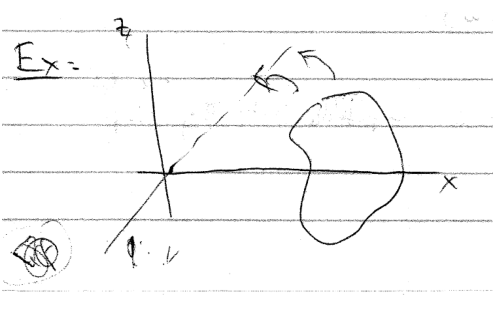
\includegraphics{drawing1.pdf}
\end{center}
We thus lead to the following parametrization: 
\begin{equation}
x=f(\phi)\cos(\theta), y=f(\phi)\sin(\theta),z=g(\phi)
\end{equation}
This space is a Riemannian manifold. Recall we have the metric inherited from $\R^{3}$:
\begin{equation}
g=dx\otimes dx+dy\otimes dy+dz\otimes dz
\end{equation}
While by our parametrization we have:
\begin{equation}
dx=f'(\phi)\cos(\theta)d\phi-f(\phi)\sin(\theta)d\theta
\end{equation}
\begin{equation}
dy=f'(\phi)\sin(\theta)d\phi+f(\phi)\cos(\theta)d\theta
\end{equation}
\begin{equation}
dz=g'(\phi)d\phi
\end{equation}
Combing together we have:
\begin{equation}
g_{M}=(f'(\phi)^{2}+g'(\phi)^{2})d\phi\otimes d\phi+f(\phi)^{2}d\theta\otimes d\theta
\end{equation}
Rearranging by letting \[\tau_{1}=\sqrt{f'(\phi)+g'(\phi)}d\phi, \tau_{2}=f(\phi)d\theta
\] we claim the above is equal to 
\begin{equation}
\tau_{1}\otimes \tau_{1}+\tau_{2}\otimes \tau_{2}
\end{equation}
To find the Levi-Civita connection we have to solve (1.22) and (1.23):
\[
d\tau_{1}=-\omega_{12}\wedge \tau_{2},
d\tau_{2}=\omega_{12}\wedge \tau_{1}
\]
for $\omega_{12}$. 

Since $M$ is a 2-dimensional manifold, we know $d\tau_{1}=0$. If we write 
\[\omega_{12}=a d\phi+bd\theta
\]
 This implies:

\begin{equation}
d\tau_{1}=-\omega_{12}\wedge \tau_{2}=(ad\phi+bd\theta)\wedge (f'(\phi)d\theta)=0
\end{equation}
When we expand it we find $\omega_{12}=bd\theta$ only. Plug into $d\tau_{2}=\omega_{12}\wedge \tau_{1}$ we have:
\begin{equation}
d\tau_{2}=F'(\phi)d\phi\wedge d\theta=bd\theta\wedge \sqrt{f'(\phi)^{2}+g'(\phi)} d\phi
\end{equation}
Resolving $b$, we conclude 
\begin{equation}
\omega_{12}=-\frac{f'(\phi)}{\sqrt{f'(\phi)^{2}+g'(\phi)^{2}}}
\end{equation}
\remark The negative sign here is questionable. \\
\bigskip
Recall $d\omega_{12}=K\tau_{1}\wedge \tau_{2}$ as we derived in (1.24). We thus conclude:
\begin{equation}
K=\frac{g'(\phi)^{2}+f''(\phi)+f'(\phi)g'(\phi)}{f(\phi)(f'(\phi)^{2}+g'(\phi)^{2})^{2}}
\end{equation}
\remark The computation at here looks fishy, I do not think it coincide with my computation. 

\section{Neat application of Levi-Civita connection}
\theorem 
\[
R(u,v)\omega+R(v,\omega)u+R(\omega,u)v=0
\]
\discussion
Recall that $\nabla^{LC}=d+\omega$, where $\omega^{T}=-\omega$, $d\tau=-\omega\wedge \tau$, and $\tau=(\tau_{1}\cdots \tau_{n})$, $\tau_{j}$s are the duals of an orthogonal trivialization of $TM$.

So we have 
\[
0=-d(\omega\wedge \tau)=d\omega \wedge \tau+(-1)\omega\wedge d\tau
\]
Rearranging and using $d\tau=-\omega\wedge\tau$ we have
\[
0=-d\omega\wedge \tau-\omega\wedge\omega\wedge tau=-(d\omega+\omega\wedge \omega)\wedge \tau=-R\wedge \tau
\]
Therefore we conclude that
\[
R\wedge \tau=0
\]

\theorem
We have
\[
R(u,v,\omega,z)=\langle R(u,v)\omega,z\rangle
\]
\example
Let $\dim M=2$, then we have
\[
\tau R\tau^{-1}=K
\begin{pmatrix}
0&1\\
-1&0
\end{pmatrix}
\tau_{1}\wedge \tau_{2}
\]
Here we have
\[
\tau=
\begin{bmatrix}
\tau_{1}\\
\tau_{2}\\
\end{bmatrix}
\]
which are dual to $e_{1},e_{2}$ that are orthogonal trivializations. 

\theorem
We have $K\equiv 0$ near a point $p\in M$ equivalent to exist coordinate system $(y_{1},y_{2})$ near $p$ such that $g=dy_{1}^{2}+dy_{2}^{2}=dy_{1}\otimes dy_{1}+dy_{2}\otimes dy_{2}$.


\chapter{The road to Gauss-Bonnet} 
\section{Definition of Differential Operators}
\definition
We define $\mbox{Diff}^{m}(U)$ as the collection of differential operators 
\[
P:C^{\infty}(U)\rightarrow C^{\infty}(U)
\]
such that
\[
P=\sum_{|I|<m}a_{I}\partial_{X_{I}},a_{I}\in C^{\infty}(U)
\]
We denote
\[
\mbox{Diff}^{0}(U)=C^{\infty}(U)
\]
and so on. Therefore
\[
\triangle\in \mbox{Diff}^{2}(U)
\]

\theorem
Let $p,Q\in \mbox{Diff}^{m}(U)$, then we have:
\begin{itemize}
\item
$P+Q\in \DIFF(U)$.

\item
$a\in C^{\infty}(U)$ implies $aP\in \DIFF(U)$.

\item
If $m\le m'$, then we have
\[
\DIFF^{m}(U)\subset \DIFF^{m'}(U)
\]
\end{itemize}

\lemma
\[
\forall a\in C^{\infty}(U),\partial_{x_{i}}\circ a=a\partial_{x_{i}}+(\partial_{x_{i}} a)
\]
This follows from Leibniz rule. 

\theorem
We have
\[
\DIFF^{m}\circ\DIFF^{n}\subset \DIFF^{m+n}
\]

\definition
We define the principal symbol. Let $P\in \DIFF^{m}(\mu)$, this implies
\[
P=\sum_{|I|\le m}a_{i}\partial_{X_{I}},a_{I}, a_{I}:U\rightarrow \C
\]
We define the principal symbol by:
\[
\sigma_{m}(P):T^{*}(U)\rightarrow \C: \xi:\sum_{|I|=m}a_{I}(q)i\xi(\partial_{x_{i1}})\cdots i\xi_{\partial_{x_{im}}}
\]
where $\xi$ is basis vector for the $T_{q}U^{*}$:
\[
\xi:T_{q}(U)\rightarrow \R
\]
We thus have
\[
\sigma_{m}(P)\in C^{\infty}(T^{*}U)
\]
Here we use the multi-symbol notation:
\[
\partial_{X_{I}}=\partial_{X_{i1}}\circ \partial_{X_{i2}}\cdots \partial_{X_{in}}
\]

\example
The Laplace operator is:

\[
\triangle=-\sum^{n}_{i=j}\partial_{x_{i}}\circ \partial_{x_{j}}
\]

\example
If $P\in \DIFF^{m}(M),Q\in \DIFF^{n}(M)$, then we have
\[
\sigma_{m+n}(P+Q)=\sigma_{m}(P)\circ \sigma_{m'}(Q)
\]

If we define $k=\max(m,n)$, then we have
\[
\sigma_{k}(P+Q)=\sigma(P)+\sigma(Q)
\]

\theorem
Let $(y_{1}\cdots y_{n})$ be another set of coordinate system on $U$, then we have
\[
P\in DIFF(U)\leftrightarrow P=\sum_{|I|\le m}b_{I}\partial_{Y_{I}}
\]
where $b_{I}\in C^{\infty}(U)$. In other words, we know 
\begin{center}
$\DIFF(U)$ is coordinate independent. 
\end{center}
\proof
Induction on $m$, for $m=0$ this is trivial. For $m=1$ we have
\[
P\in \DIFF(U)\leftrightarrow P=\sum_{|I|\le 1}a_{I}\partial X_{I}=a_{0}+\sum^{n}_{j=1}a_{j}\partial_{x_{j}}
\]
and the rest follows from chain rule. Then we induct. 

\theorem
The principal symbol $\sigma$ is coordinate independent. 

\proof
This is left as an excise. 

Now we have seen that
\begin{itemize}
\item
$\DIFF(U)$ is coordinate independent. 

\item
for $m\le n$, we have
\[
\DIFF^{m}\subset \DIFF^{m-1}
\]
Let $\sigma_{m}(P)=T^{*}(U)\rightarrow \C$. Then we have
\[
\sigma_{m}(P)(\xi)=i^{m}\sum_{|i|=m}a_{I}\xi(\partial_{i})\cdots \xi(\partial_{k})
\]
Here we have
\[
\sigma_{m}(P)\in C^{\infty}(T^{*}U)
\]
\end{itemize}
\theorem
We have the following exact sequence:

\[
0\rightarrow \DIFF^{m-1}\rightarrow \DIFF^{m}\rightarrow^{\sigma_{m}}C^{\infty}(T^{*}(U))\rightarrow 0
\]
Also we know that $\sigma_{m}(P)$is coordinate free. We have:

\[
\sigma_{m+n}(P\circ Q)=\sigma_{m}(P)\circ \sigma_{n}(Q)
\]

\section{Differential Operator on Manifolds}
Let $M$ be a $C^{\infty}$ manifold. Given $m\in \{0,1,2\cdots \}$, a $m$-th order differential operator is a linear map
\[
P:C^{\infty}(M)\rightarrow C^{\infty}(M)
\]
such that
\[
\forall u\in C^{\infty}(M),\forall \mbox{coordinate patch} U\subset M
\]
We have
\[
P_{u}|_{U}=P_{u}(u|U), P_{u}\in \DIFF^{m}(M)
\]
such that we have
\[
(Pu)_{U}=\sum_{|I|\le m}a_{I}\partial_{X_{I}}(u|U), \mbox{for some} a_{I}\in C^{\infty}(U)
\]
It satisfies the following properties:
\begin{itemize}
\item
$$\DIFF^{m}(M)\circ \DIFF^{n}(M)\subset \DIFF^{m+n}(M)$$
\item
$\DIFF^{m}(M)$ is a module over $C^{\infty}(M)$.
\end{itemize}

\discussion
We now re-visit the principal symbol. Let $P\in \DIFF(M)$, we define
\[
\sigma_{m}(P):T^{*}(M)\rightarrow \C
\]
as follows:
Take any coordinate patch $U$ containing $q$ and let 
\[
P_{u}:\mbox{local representation of}P \mbox{over} U
\]
Then we have
\[
\sigma_{m}(P)(\xi)=\sigma_{m}(P_{u})(\xi)\in \C
\]
\lemma
Properties of the principal symbol:
\begin{itemize}
\item
\begin{center}
$
\sigma_{m}(aP_{1}+bP_{2})=a\sigma_{m}(P_{1})+b\sigma_{m}(P_{2})$
\end{center}
\item
\[
\sigma_{m+n}(P\circ Q)=\sigma_{m}(P)\times \sigma_{n}(Q)
\]
\end{itemize}

\lemma
We have the adjointness over Hermitian product spaces:
Let $T:V\rightarrow W$ be a linear map, then its adjoint (if it exists) is a linear map $A:W\rightarrow V$ such that
\[
\langle TV,W\rangle=\langle V,AW\rangle,\forall v\in V,w\in W
\]

\definition
The adjoint is unique and denoted by $T^{*}$. 

\lemma
We define an inner product by assuming $M$ is an oriented Riemannian compact manifold. Let $dg$ be the volume form. Then we have
\[
\int:C^{\infty}(M)\rightarrow \C:f\rightarrow \int fdg
\]
So we have the inner product defined by the $L^{2}$ fashion:
\[
\langle f,g \rangle:C^{\infty}(M)\times C^{\infty}(M):
\int_{M}f\overline{h}dg
\]

\theorem Any $P\subset \DIFF^{m}(M)$ have an adjoint. In other words, there exists 
$$
P^{*}:C^{\infty}(M)\rightarrow C^{\infty}(M)
$$
such that
$$
\langle Pf,h\rangle=\langle f,P^{*}h\rangle
$$
Moreover we know that
$$
P^{*}\in \DIFF(M)
$$
and we have
$$
\sigma_{m}(P)=\overline{\sigma_{m}(P)}
$$
To prove it we use integration by parts:
$$
\int(\partial_{x_{j}}f)\overline{h}=-\int f\overline{\partial_{x_{j}}h}
$$

We now discuss the case on vector bundles. 

\example
We consider the trivial case on the exterior form bundle. We have
$$
d:C^{\infty}(M,\wedge^{k})\rightarrow C^{\infty}(M,\wedge^{k+1})
$$
such that
$$
(d\alpha)|_{\mu}=\sum \frac{\partial \alpha_{J}}{x_{j}}dx_{j}\wedge dx_{J}
$$
where
$$
\alpha|_{\mu}=\sum a_{J}dx_{J}\in C^{\infty}(U)
$$

\example
We consider the case of the covariant derivative. We have
$$
\nabla:C^{\infty}(M,E)\rightarrow C^{\infty}(M,\wedge^{1}\otimes E)
$$
such that 
$$
(\nabla e)|_{U}=\sum \frac{\partial \alpha_{j}}{\partial x_{k}}dx_{k}\otimes e_{j}+\sum b^{k}_{ij}a_{j}dx_{k}\otimes e_{i}
$$
Here we have
$$
\sum b_{ij}dx_{k}=w_{ij}\in C^{\infty}(M,\wedge^{1}),e|_{U}=\sum a_{j}e_{j}
$$
We can also re-write this as
$$
(\nabla e)_{U}=\sum_{k,i}(\sum_{j}\delta_{ij}\frac{\partial}{\partial x_{j}}+b^{k}_{ij})a_{j}dx_{k}\otimes e_{j}
$$
That's how we get
$$
\nabla=d+w
$$
If we regard
$$
P_{k,i}=\sum_{j}\delta_{ij}\frac{\partial}{\partial x_{j}}+b^{k}_{ij}
$$
as a differential operator indexed by $k,i$, we have each term being a first order differential operator:
$$
P_{k,i}(j)=\delta_{ij}\frac{\partial}{\partial x_{j}}+b^{k}_{ij}\in \DIFF^{1}(\mu)
$$

\example
We have
$$
(d\alpha)|_{U}=\sum_{j,J}\frac{\partial \alpha_{J}}{\partial x_{j}}dx_{j}\wedge dx_{J}
$$
where we assume
$$
\alpha|_{U}=\sum \alpha_{J}dx_{J}
$$
we note that the basis over $\wedge^{k}$ is $dx_{J}$. We finally note:

$$
(d\alpha)_{U}=\sum_{i,J,I}\frac{\alpha_{J}}{\partial x_{j}}sgn((i,J),(j,J))dx_{I}
$$
where
$$
sgn((i,J),I)
$$
will be defined later. 

\section{Differential Operator On Manifolds, II}
$\DIFF(M)$ consists of linear maps
$$
P:C^{\infty}(M)\rightarrow C^{\infty}(M)
$$
such that for any coordinate patch $\mathcal{M}\subset M$, there exist $P_{U}\in \DIFF^{m}(M)$, such that
$$
\forall \mu \in C^{\infty}(M), (P\mu)|_{U}=P_{\mu}(U|_{U}
$$

Assuming that $M$ is a Riemannian compact oriented manifold. Recall that, given $P\in \DIFF^{m}(M)$, a coordinate cover $\{U_{j}\}$ of $M$, and a coordinate partition subordinate to $\{U_{j}\}$, the operator
$$
Q=\sum_{j}\phi_{j}Q_{j}
$$
where
$$
Q_{j}=(P_{U_{j}}^{*}
$$
satisfies
$$
\langle Pu,v\rangle=\rangle u,Qv\rangle, \forall u,v\in C^{\infty}(M)
$$

Therefore, given $\mu\in C^{\infty}(M)$, we have
$$
Q(\mu)=\sum_{j}\phi_{j}Q_{j}(\mu|_{U_{j}})\in C^{\infty}(M)
$$
To discuss other topics we need the following theorem:

\theorem
Let $U,V$ be overlapping coordinate patches, let $\phi\in C^{\infty}_{c}(U)$. 

\begin{itemize}
\item
If $v\in C^{\infty}(U\cap V)$, then $\phi(v)\in C^{\infty}(V)$. 

\item
If $P\in \DIFF^{m}(U)$, then 
$$
\phi P\in \DIFF^{m}(V)
$$
\end{itemize}
\proof
Exercise. We note that $\phi(v)$ could be extended by $0$ trivially in $V$.

Using this theorem, we can prove that any coordinate patch $V\subset M,\forall j$, $v\in C^{\infty}(V)$, we have
$$
\phi_{j}Q_{j}(v)\in C^{\infty}(V)
$$
Therefore
\begin{center}
$Q$ satisfies the definition of $\DIFF^{m}(M)$ and $Q\in \DIFF^{m}(M)$. 
\end{center}

\section{Vector Bundles}
Let $V,W$ be vector spaces. Let $T:V\rightarrow W$ be linear map such that
$$
Te_{j}=T_{ij}f_{i}
$$

\theorem
We have
$$
T:V\rightarrow W \in Hom(V,W)\leftrightarrow \exists \alpha_{i}\in V^{*},\exists w_{i}\in W^{*}
$$
and constants $\tau_{ij}$, such that we have
$$
\forall e\in V, T(e)=\sum_{i,j}\tau_{ij}\alpha_{j}(e)w_{i}
$$
\proof
This is clear. 

Let $E,F$ be complex vector bundles over $M$. We define

$$
\DIFF^{m}(M,E,F)=\{P:C^{\infty}(M,E)\rightarrow C^{\infty}(M,F)\}
$$
such that for any coordinate patch, exists a trivialization
$$
e_{1}\cdots e_{N_{1}}\in E_{U}, f_{1}\cdots f_{N_{2}}\in F_{U}
$$
and
$$
P_{ij}\in \DIFF^{m}(U)
$$
such that
$$
(Pe)|_{U}=\sum (P_{ij}\alpha_{j})f_{i},e|_{U}=\sum a_{j}e_{j}
$$

\example
We consider the trivial example. We have
$$
d:C^{\infty}(M,\wedge^{k})\rightarrow C^{\infty}(M,\wedge^{k+1})
$$

Let $U$ be a coordinate patch and $\alpha \in C^{\infty}(M,\wedge^{n})$. We have
$$
\alpha|_{U}=\sum_{J}\alpha_{J}dx_{J},i\le j_{1}\le j_{2}\cdots j_{n}\le n
$$
We thus have
$$
(d\alpha)|_{U}=\sum_{j,J}\frac{\partial \alpha_{j}}{\partial x_{J}}dx_{j}\wedge dx_{J}
$$
But it does not satisfy the description earlier, because $dx_{j}\wedge dx_{J}$ is not a basis itself. 

To solve this problem we define

$$
(d\alpha)_{U}=\sum_{i,j,I}sgn((i,J),J)\frac{\partial \alpha_{J}}{\partial x_{j}}dx_{J}, 1\le i_{1}<i_{2}\cdots <i_{n}<n
$$
\remark I think here is a typo in the notes, the $x_{J}$ in the notes is $x_{I}$, which does not make sense here. We continue with the example:

\proof
So we have
$$
(d\alpha)|_{U}=\sum_{I}\sum_{J}(P_{IJ}\alpha_{J})dx_{I}
$$
where we have
$$
P_{IJ}=\sum^{n}_{j=1}syn((i,J),I)\partial x_{j}
$$
Now we have
$$
d\in \DIFF^{1}(M,\wedge^{k},\wedge^{k+1})
$$

\example
We now revisit the covariant derivative. We have
$$
\nabla(e)|_{U}=\sum da_{j}\otimes e_{j}|_{U}+\sum a_{j}(\nabla e_{j})|_{U}
$$

and we have
$$
(\nabla e_{j})_{U}=\sum_{k,i}b^{k}_{ij}dx_{k}\otimes e_{i}, b^{k}_{ij}\in C^{\infty}(U)
$$

Thus
$$
(\nabla e)|_{U}=\sum \frac{\partial a_{j}}{\partial x_{k}}dx_{k}\otimes e_{i}+\sum_{i,j,k}\sum^{k}_{i,j}a_{j}dx_{k}\otimes e_{i}
$$

\remark
I think Maurcio lost $a_{j}$ in the formula. I add it for completeness. 

\proof

which equals

$$
\sum_{k,i}(\sum_{j}\delta_{ij}\frac{\partial}{\partial x_{j}}+b^{k}_{ij})a_{j}dx_{k}\otimes e_{j}=\sum_{k,i,j}(P_{k,i,j}a_{j})dx_{k}\otimes e_{i}
$$
where
$$
P_{k,i,j}=\delta_{jk}\frac{\partial}{\partial x_{k}}+b^{k}_{ij}\in D^{1}(M)
$$
therefore
$$
\nabla\in \DIFF^{1}(M,E,\wedge^{1}\otimes E)
$$

\section{Adjoints}
Assume that $E,F$ are Hermitian vector bundles. Given $e_{1},e_{2}\in C^{\infty}(M,E)$, we have

$$
( e_{1},e_{2}) \in C^{\infty}(M)
$$
defined pointwise. We assume $M$ is a Riemannian, compact, oriented manifold such that
$$
\langle e_{1},e_{2}\rangle=\int_{M}(e_{1},e_{2})dg
$$

Let $P\in \DIFF^{m}(M,E,F)$ such that
$$
P:C^{\infty}(M,E)\rightarrow C^{\infty}(M,F)
$$
recall the definition of the adjoint for vector spaces. We have the similar definition for vector bundles. Using it we have the following theorem:

\theorem
Given $P\in \DIFF^{m}(M,E,F)$, it has an adjoint
$$
P^{*}:C^{\infty}(M,F)\rightarrow C^{\infty}(M,E)
$$
Moreover, we have
$$
P^{*}\in \DIFF^{m}(M,F,E)
$$

\section{Principal Symbol}
We now review the principal symbol. We have
$$
\DIFF^{m-1}(M,E,F)\rightarrow \DIFF^{m}(M,E,F)
$$
What is the quotient 
$$
\DIFF^{m}(M,E,F)/\DIFF^{m}(M,E,F)?
$$
Given
$$
P\in \DIFF^{m}(M)
$$
recall that for all
$\xi\in T^{*}_{q}M$ we have
$\sigma_{m}(P)(\xi)\in \C$. We now have
$$
\sigma_{m}(P)(\xi)=\sigma_{m}(P_{U})(\xi)
$$
after restricting to a coordinate patch. Now let
$$
P\in \DIFF^{m}(M,E,F)
$$
and
$$
\xi\in T^{*}_{q}(M)
$$
We choose a coordinate patch $U$ with $f\in U$ and choose coordinate functions $e_{i},f_{i}$ so that we have
$$
P=\sum P_{ij}e_{j}^{*}\otimes f_{i}
$$
We have
$$
\sigma_{m}(P)(\xi)=\sum_{i,j}\sigma_{m}(P_{ij})(\xi)e_{j}^{*}\otimes f_{i}(q),\in Hom(E_{q},F_{q})
$$
where of course
$$
e_{j}^{*}\otimes f_{i}(q)\in Hom(E,F)
$$
and
$$
\sigma_{m}(P_{ij})
$$
is a polynomial of $\xi$.We can thus conclude that

$$
\sigma_{m}(P):T_{q}^{*}(M)\rightarrow Hom(E_{q},F_{q})
$$
but actually we have something stronger:
$$
\sigma_{m}(P):T^{*}(M)\rightarrow Hom(E,F)
$$
between bundles. Note that if $e\in E_{q}$, then we can write
$$
e=\sum a_{j}e_{j}(q),a_{j}\in \C
$$
Then we have
$$
\sigma_{m}(P)(\xi)\in Hom(E_{p},E_{q})
$$
and
$$
\sigma_{m}(P)(\xi)(e)=\sum \sigma_{m}(P_{ij})(\xi)a_{j}f_{j}(q)
$$

\example
We consider the familiar example $d$ and $\nabla$. We have
$$
\sigma_{1}(\xi)(e)=\sum_{k,i,j}\sigma_{1}(P_{k,i,j})(\xi)(e)dx_{k}\otimes e_{i}
$$
which equals
$$
i\sum \delta_{j,k}\xi(\partial x_{k})dx_{k}\otimes e_{i}
$$
After equating $\partial_{x_{k}}(dx_{k})=1$ we have
$$
i\xi\otimes e
$$ 
This is clear, for example from the definition of $\nabla=d+\omega$, and we know the principal symbol of $d$ is
$$
\sigma_{1}(d)(\xi)=i\xi
$$

\section{Reivew of previous section}

Let $P\in \DIFF^{m}(M,E,F)$, this implies
$$
P:C^{\infty}(M,E)\rightarrow C^{\infty}(M,F)
$$
The map is linear over $\C$ and valid over any coordinate patch $U$ and trivialization $e_{1}\cdots e_{N};f_{1}\cdots f_{N}$ of $E_{U},F_{U}$ respectively. We now have

$$
P|_{U}=\beta^{-1}[P_{ij}]\alpha, \alpha=[e_{1}^{*}\cdots e_{N}^{*}]^{T},\beta=[f_{1}^{*}\cdots f_{N}^{*}]^{T}
$$
such that for all $e\in C^{\infty}(M,E)$, we have
$$
Pe|_{U}=\sum (P_{ij}a_{j})f_{i}, e|_{U}=\sum a_{j}e_{j}
$$
Note that we have
$$
P|_{U}=\sum P_{ij}e_{j}^{*}\otimes f_{i}
$$
We also have
$
P\in \DIFF^{m}(M,E,F)
$ implies
$P|_{U}=\sum P_{ij}\alpha_{j}\otimes g_{i}$ for some $\alpha_{j}\in C^{\infty}(U,E^{*})$, $g_{*}\in C^{\infty}(U,F)$.
Then we have
$$
P_{ij}\in \DIFF^{m}(U)
$$

\example
We consider the known example. We have
$$
\nabla:C^{\infty}(E)\rightarrow C^{\infty}(M,\C\wedge^{1}\otimes E)
$$
and we know
$$
\nabla(e)=\sum_{k,i}\sum_{j}(\delta_{i,j}\partial_{x_{k}}+b^{n}_{ij})a_{j}dx_{k}\otimes e_{i}
$$
If we assume
$$
e|_{U}=\sum a_{j}e_{j}
$$
Then we would have
$$
\nabla e_{j}=\sum b^{n}_{ij}dx_{k}\otimes e_{i}
$$
\remark
I think Maurcio has a typo here, $e_{j}$ in his equation should be $e_{i}$. We continue. 

\proof
which equals
$$
\sum_{k,i,j}(P_{k,i,j}a_{j})dx_{k}\otimes e_{i}
$$
where
$$
P_{k,i,j}=\delta_{i,j}\partial_{x_{k}}+b^{k}_{ij}\in C^{\infty}(U)
$$
as before. 

\remark
Why should $\delta_{i,j}\partial_{x_{k}}$ in $C^{\infty}(U)$?

We now have
$$
(\nabla e)|_{U}=\nabla(\sum a_{j}e_{j})=\sum da_{j}\otimes e_{j}+a_{j}\nabla e_{j}=\sum \frac{\partial a_{j}}{\partial x_{k}}dx_{k}\otimes e_{j}+\sum_{j}^{n}a_{j}\sum^{n}_{k,i}b^{k}_{ij}dx_{k}\otimes e_{i}
$$
Rearranging we have this equal to
$$
(\sum_{i,j,k}\partial_{k}e_{j}^{*}\otimes (dx_{k}\otimes e_{j})+\sum b^{k}_{ij}e^{*}_{j}\otimes dx_{k}\otimes e_{i})
$$

\example
We now revisit another familiar example. We have
$$
d:C^{\infty}(M,\wedge^{k})\rightarrow C^{\infty}(M,\wedge^{k+1})
$$
\remark I think there is a typo in Maucrio's notes. We continue.

\proof
We thus have
$$
(d\alpha)|_{U}=\sum sgn((j,J),I)\frac{\partial \alpha_{J}}{\partial x_{j}}dx_{I}
$$
Here we assume
$$
\alpha|_{U}=\sum \alpha_{J}dx_{J}=\sum_{I,J}(P_{IJ}\alpha_{J})dx_{I},P_{IJ}=\sum sgn(j,J)\partial_{j}
$$
\remark
I think there is another typo here, we cannot have
$$
\partial_{j}a_{J}
$$
appeared in the summation. We continue. 

\proof
Therefore we have
\begin{align}
d\alpha&=\sum \partial_{j}\alpha_{J}dx_{j}\wedge dx_{J}\\
&=\sum \partial_{x_{j}}(dx_{J})\otimes (dx_{j}\wedge dx_{J})\\
&=\sum (\DIFF^{1})\alpha_{J}\otimes g_{i,J}
\end{align}
\remark
I think (2.2) and (2.3) does not make much sense. The equation need some heavy editing. We continue. 

\proof
We thus conclude that $d$ is a differential operator. 

\definition
We define a differential operator on $U$ as 
$$
P|_{U}=\beta^{-1}[P_{ij}]\alpha
$$
and
$$
\sigma_{m}(P)(\xi)=\beta_{q}^{-1}(\sigma_{m}(P_{ij})(\xi))\alpha_{q}:E_{q}\rightarrow F_{q}
$$
Also, if 
$$
P|_{U}=\sum Q_{ij}\alpha_{j}\otimes g_{i}\in C^{\infty}(M,F), Q_{ij}\in C^{\infty}(M,E)
$$
We then have
$$
\sigma_{m}(P)(\xi)=\sum \sigma_{m}(Q_{ij})(\xi)\alpha_{j}(q)\otimes g_{i}(q):E_{q}\rightarrow E_{q}
$$
We note that
$$
\sigma_{m}(P)\in C^{\infty}(T^{*}M, Hom(E,F))
$$
and it is fiber preserving. 

\example
We now revisit our example earlier:
We have
$$
\sigma_{1}(\nabla)(\xi)=i\xi
$$
because we have
$$
\nabla=\sum \partial_{k}e_{j}^{*}\otimes (dx_{k}\otimes e_{j})+\triangle
$$
where the $\triangle$ denotes lower order terms from $\omega$ we ignore. We now have
$$
\sigma_{1}(\nabla)(\xi)=\sum i\xi(\partial_{k})e_{j}^{*}\otimes dx_{k}\otimes e_{j}
$$
But know that
$$
\xi=\sum \xi(\partial_{k})dx_{k}
$$
and
$$
id_{E}=\sum e_{j}^{*}\otimes e_{j}
$$
Therefore we have
$$
\sigma_{1}(\nabla)(\xi)=i\xi\otimes id:E\rightarrow \C\wedge^{1}\otimes E 
$$

\example
Similarly we have
$$
\sigma_{1}(d)(\xi)=\sum i\xi(\partial_{j})(dx_{J})^{*}\otimes dx_{j}\wedge dx_{J}
$$
Using the fact that
$$
\xi=\sum \xi(\partial_{j})dx_{j}
$$
We have
$$
\sigma(d)(\xi)=i\xi\wedge:C\wedge^{k}\rightarrow \C\wedge^{k+1}
$$

\section{Adjoints, Review}
Recall that if we assume $M$ is compact, oriented Riemannian manifold and $\langle \rangle$ is a Hermitian inner product. Then we have
$$
C^{\infty}(M,E)\times C^{\infty}(M,E)\rightarrow \C
$$
such that
$$
(e_{1},e_{2})=\int \langle e_{1},e_{2}\rangle dg
$$

\theorem
For all $P\in \DIFF^{m}(M,E,F)$, there exist $P^{*}\in \DIFF^{m}(M,F,E)$ such that
$$
(Pe,f)=(e,P^{*}f),\forall e\in C^{\infty}(M,E), f\in C^{\infty}(M,F)
$$
such that
$$
P:C^{\infty}(M,E)\rightarrow C^{\infty}(M,F)
$$
has a formal adjoint
$$
P^{*}:C^{\infty}(M,F)\rightarrow C^{\infty}(M,E)
$$
Moreover we have
$$
\sigma_{m}(P^{*})(\xi)=\overline{\sigma_{m}(P)(\xi)}
$$
Recall that
$$
\sigma_{m}(P)(\xi):E_{q}\rightarrow F_{q}
$$
and
$$
\sigma_{m}(P^{*})(\xi)=\textrm{adjoint}
$$

\example
We have
$$
d:C^{\infty}(M,\C\wedge^{k})\rightarrow C^{\infty}(M,\C\wedge^{k+1})
$$
so we have
$$
d^{*}:C^{\infty}(M,\C\wedge^{k+1})\rightarrow C^{\infty}(M,\C\wedge^{k})
$$
Therefore we have
$$
\sigma(d^{*})(\xi)=(\sigma_{1}(d)(\xi))^{*}=(i\xi\wedge )^{*}=-(i\xi\wedge )^{*}
$$
\lemma
We claim that the adjoint of 
$$
\xi\wedge :\C\wedge^{k}\rightarrow C\wedge^{k+1}
$$
is
$$
\beta^{\#}\rfloor
$$
So we have
$$
\sigma_{1}(d^{*})(\xi)=-i\xi^{\#}\rfloor
$$
\example
For any $\alpha \in \wedge^{k}_{q}$, we have
$$
\langle \xi\wedge \alpha,\beta\rangle=\langle \alpha,\xi^{\#}\rfloor\beta\rangle
$$
\example{\bf The Hodge Star}\\
Now consider
$$
D=d+d^{*}:C^{\infty}(M,E)\rightarrow C^{\infty}(M,E)
$$
Here $E$ is the exterior form bundle
$$
\C\wedge^{0}\otimes \cdots \C \wedge^{n}
$$
Then $D\in \DIFF^{1}(M,E)$ and $$\sigma_{1}(D)(\xi)=i(\xi\wedge^+-\xi^{\#}\rfloor):E\rightarrow E$$
When composed twice we have:
$$
\sigma_{1}(D)(\xi)\circ \sigma_{1}(D)(\xi):E\rightarrow E
$$
can be computed directly by
$$
\xi^{\#}(\xi)=\langle \xi,\xi \rangle
$$
This example motivate the following definition:

\definition Let $E$ be any complex hermitian vector bundle and $D\in \DIFF^{1}(M,E)$. Then $D$ is a $\textbf{Dirac Operator}$ if $D$ is self adjoint ($D^{2}=D$) and 
$$
\sigma_{1}(D)(\xi)^{2}=|\xi|^{2}
$$

\section{Index of a Dirac Operator}
Now let $D$ be a Dirac operator:
$$
D:C^{\infty}(M,E)\rightarrow C^{\infty}(M,E)
$$
and assume $E$ is $\Z_{2}$ graded: $E=E^{+}\oplus E^{-},\dim E^{+}=\dim E^{-}$. Assume that
$$
D:C^{\infty}(M,E^{\pm})\rightarrow C^{\infty}(M,E^{\mp}) 
$$
In other words, we have:
$$
Z:E\rightarrow E
$$
by
$$
Z=
\begin{cases}
1 & \mbox{on} E^{+}\\
-1 & \mbox{on} E^{-}\\
\end{cases}
$$
Then we have $D\circ Z=-Z\circ D$. 
\example
If $e\in E^{+}$, we have:
$$
D\circ Z(e)=D(e)=-Z\circ (D)=-Z(D(e))=D(e)
$$
\example
Let $E=\C\wedge^{*}=\C\wedge^{even}\oplus \C \wedge^{odd}$ and $\dim M$ is even. Then we can define
$$
D^{+}=D:C^{\infty}(M,E^{+})\rightarrow C^{\infty}(M,E^{-})
$$
and
$$
D^{-}:D:C^{\infty}(M,E^{-})\rightarrow C^{\infty}(M,E^{+})
$$
Here our $D^{\pm}$ is the adjoint of $D^{\mp}$. In other words
$$
(D^{+}(e),f)=(e,D^{-}(f))
$$

\remark I belive Prof. Loya used $D$ as map between $E^{+}_{m}$ and $E^{-}_{m}$ fiber wise once we fixed $m$, not literally a map on sections. 

\theorem
$D^{+}=D:C^{\infty}(M,E^{+})\rightarrow C^{\infty}(M,E^{-})$ is Fredholm. This means:
\begin{itemize}
\item
$\dim \ker D^{+}<\infty$
\item
$\dim \textrm{coker} D^{+}<\infty$
\end{itemize}

\definition 
We define the $\textbf{index}$ of a differential operator by
$$Ind D^{+}=\dim \ker D^{+}-\dim \textrm{coker} D^{+}$$

\section{Hodge decomposition Theorem}
Let $M$ be a compact, oriented Riemannian manifold. Let $P:C^{\infty}(M,E)\rightarrow C^{\infty}(M,E)$ be an elliptic differential operator. Let $E,F$ be Hermitian vector bundles over $M$. 

\theorem
$
P:C^{\infty}(M,E)\rightarrow C^{\infty}(M,F)
$ is Fredholm. Moreover, we have:
\begin{itemize}
\item
$\dim \ker P<\infty$
\item
$\dim \ker P^{*}<\infty$
\item 
$C^{\infty}(M,F)=PC^{\infty}(M,E)\oplus \ker P^{*}$.
\end{itemize}
We will prove the above theorem in the case $P=D$, a generalized Dirac operator. We review the theorem's application when $P=D=d+d^{*}$:

\lemma
We have
$$
D:d+d^{*}:C^{\infty}(M,\wedge^{*})\rightarrow C^{\infty}(M,\wedge^{*})
$$
Then $\dim \ker D<\infty$ and
$$
C^{\infty}(M,\wedge^{*})=DC^{\infty}(M,\wedge^{*})\oplus \ker D
$$
This is the $\textbf{Hodge decomposition}$.

\corollary
We have
$$
\ker D\cong H^{*}_{DR}(M)
$$
We note that
$$
D^{2}=\triangle
$$
is the Laplace-Beltrami operator, and $\ker D\cong \ker D^{2}\cong H^{*}_{DR}(M)$. 

\proof
Let $\alpha\in \ker D$. This implies $\alpha\in C^{\infty}(M,\wedge^{*})$ with
$$
d\alpha+d^{*}(\alpha)=0\rightarrow d^{*}d\alpha+{d^{*}}^{2}\alpha=0\rightarrow d^{*}d\alpha=0 \label{hodge}
$$
We construct a map
$$
\alpha\rightarrow [\alpha]\in H^{*}_{DR}
$$
We have to verify the map is well defined. We note that $d\alpha=0$ if and only if
$$
(d\alpha,d\alpha)=(\alpha,d^{*}d\alpha)=0 
$$ but we know $d^{*}d\alpha=0$. 
This implies
$$
\alpha\rightarrow [\alpha]\in H_{DR}^{*}(M)
$$
is well defined. We now prove it is indeed an isomorphism. Let $\alpha,\beta\in \ker D$ such that $\alpha\not=\beta$. If $\alpha=\beta+d\gamma$, then we have
$$
D\alpha=D(\beta+d\gamma)=0\leftrightarrow Dd\gamma=0\leftrightarrow d^{*}d\gamma=0
$$
Therefore
$$
\langle d\gamma+d^{*}\gamma,d\gamma+d^{*}\gamma\rangle=2\langle \gamma,dd^{*}\gamma\rangle=0\rightarrow \gamma\in \ker D
$$
By our reasoning earlier we then have $d\gamma=0$. Therefore the map
$$
\alpha\rightarrow [\alpha]
$$
is unique. We also have to prove it is surjective. Let $a\in H^{*}_{DR}(M)\not=0$, we must show that $a\in \ker(D)$.
By Hodge decomposition Theorem we may decompose $a=a_{1}+a_{2}$, where $a_{1}=D(\beta)\in DC^{\infty}(M,\wedge^{*})$. Then we have
$$
da=0\leftrightarrow da_{1}=0\leftrightarrow (dd+dd^{*})\beta=0\leftrightarrow dd^{*}(\beta)=0\leftrightarrow D\beta=0\leftrightarrow a_{1}=0
$$
So we concluded the isomorphism. 

\discussion
We now wish to prove Hodge decomposition under assumptions that $\D$ is a Dirac operator, $E$ is $\Z_{2}$-graded with $Z$ defined earlier. So
$$
\D:C^{\infty}(M,E^{\pm})\rightarrow C^{\infty}(M,E^{\mp})
$$
Before we prove it we provide a few examples. 

\example
$$
\D=d+d^{*}:C^{\infty}(M,E^{\pm})\rightarrow C^{\infty}(M,E^{\mp}),\wedge^{*}=\wedge^{even}\oplus \wedge^{odd}
$$

\example
$$
M=\R^{2},\D=
\begin{pmatrix}
0 & \OP^{*}\\
\OP& 0
\end{pmatrix}:C^{\infty}(\R^{2},\C\times \R^{2})\rightarrow C^{\infty}(\R^{2},\C\times \R^{2})
$$
Here
$$
\OP=\partial_{x}+i\partial_{y},\OP^{*}=\partial_{x}-i\partial_{y}
$$
and
$$
\sigma(D)(\xi)^{2}=[i
\begin{bmatrix}
0& -\xi(\partial_{x}+i\xi(\partial_{y})\\
\xi(\partial_{x})+i\xi(\partial_{y})& 0
\end{bmatrix}]^{2}=|\xi|^{2}
\begin{pmatrix}
1 &0\\
0 & 1
\end{pmatrix}
$$
\remark
I think this is the example of a Cauchy-Riemann operator. 
\discussion
In general, we can always write
$$
\D=
\begin{pmatrix}
0& \D^{-}\\
\D^{+} & 0
\end{pmatrix}:C^{\infty}(M,E^{+}\oplus E^{-})\rightarrow C^{\infty}(M,E^{+}\oplus E^{-})
$$
We will now compute the index of $\D^{+}$. Recall by Theorem 19 for $P$ elliptic, we have
$$
ind P=\dim \ker P-\dim \ker P^{*}
$$
\lemma
In our case it translates to
$$
ind D^{+}=\dim \ker D^{+}-\dim \ker D^{-}
$$
because $\D$ is self-adjoint. 

\proof
We can prove this using Hodge decomposition:
$$
C^{\infty}(M,E)=\D C^{\infty}(M,E)\oplus \ker \D
$$
which showed $\textrm{coker}\D^{+}=\ker D^{-}$.
\remark
The index of $\D$ is zero, so we are only interested in the index of $\D^{+}$. 

\lemma
Recall $\D\circ Z=-Z\circ \D$, we have:
$$
ind \D^{+}=sgn(Z:\ker \D\rightarrow \ker \D)=\# \textrm{positive eigenvalues - negative eigenvalues of $Z$}
$$
where $Z$ acts on $\ker \D\cong H^{*}_{DR}(M)$. 

\example
We have
$$
d+d^{*}:C^{\infty}(M,\C\wedge^{*})\rightarrow C^{\infty}(M,\C\wedge^{*}), E=\C\wedge^{*}=\C\wedge^{even}\oplus \C\wedge^{odd}
$$
So we have
$$
Ind D^{+}=syn(Z:H^{*}_{DR}(M)\rightarrow H^{*}_{DR}(M))=\chi(M)
$$
where 
$$
Z=\begin{cases}
1 & \mbox{on even forms}\\
-1 & \mbox{on odd forms}
\end{cases}
$$

\remark
Many nice objects can be written in terms of the indexes of the Dirac operator.

\section{Determinants and Traces}
Let $V$ be a finite dimensional vector space. We have
$$
\det:Hom(V)\rightarrow \C
$$
Here if we write
$$
f\in Hom(V)=\sum a_{ij}v_{i}\otimes v_{j}
$$
Then we have
$$
\det(f)=\sum_{\sigma}sgn(\sigma)a_{i\sigma(1)}\cdots a_{n\sigma(n)}
$$
Now let $\mathcal{A}$ equal to a commutative algebra over $\C$. We have:
$$
\det:\mathcal{A}\otimes Hom(V)\rightarrow \mathcal{A};Tr:\mathcal{A}\otimes Hom(V)\rightarrow \mathcal{A};
$$
If $f\in \mathcal{A}\otimes Hom(V)$, then we have:
$$
f=\sum a_{ij}\otimes v_{i}\otimes v_{j}^{*}
$$
and we have
$$
\det(f)=\sum_{\sigma}sgn(\sigma)a_{i\sigma(1)}\cdots a_{n\sigma(n)}
$$
\section{$\hat{A}$-genus}
Let $\A_{0}$ be a nilpotent algebra over $\C$. This means that there exist $n_{0}\in \N$ such that
$$
\prod^{K}_{i=1}a_{i}=0,\forall a_{i}\in A,K>n_{0}
$$

\example
Consider
$$
\A_{0}=\C\wedge^{2}_{p}\oplus \C\wedge^{4}_{p}\oplus \cdots \C\wedge^{2m}_{p},2m=\dim M
$$
Here we let
$$
\A=\C\oplus \A_{0}
$$
or 
$$
\A=\C\wedge^{\textrm{even}}_{p}
$$

\discussion Consider
$$
\frac{z}{\sinh(z)}=1+\sum^{\infty}_{k=1}b_{k}z^{2k}
$$
Let $T\in \A_{0}\otimes Hom(V)$, then we have
$$
\frac{T}{\sinh(T)}=1+\sum^{\infty}_{k=1}b_{k}T^{2k}\in \mathcal{A}\otimes Hom(V)
$$
because the second term is in $\mathcal{A}_{0}\otimes Hom(V)$. This implies
$$
\det(\frac{T}{\sinh(T)})\in \A
$$
by out discussion earlier in 2.11. We now consider
$$
(1+z)^{1/2}=1+\sum^{n_{0}}_{k=1}{\frac{1}{2}\choose k}z^{k}
$$

\example
Let
$$
\det(\frac{T}{\sinh(T)})=1+\beta, \beta\in \A_{0}
$$
Then we have
$$
\sqrt{\det(\frac{T}{\sinh(T)})}=(1+\beta)^{1/2}=1+\sum^{n_{0}}_{i=1}{\frac{1}{2}\choose k}\beta^{k}\in \C\oplus\A_{0}=\A
$$
This implies that
\[
\displaystyle\hat{A}(T)=(\det)^{\frac{1}{2}}(\frac{T}{\sinh(T)})\in\A
\]

\section{Relative Chern Character}
Let $S\in Hom(V)$ and $T\in \A_{0}\otimes Hom(V)$. We have
$$
e^{z}=1+\sum^{\infty}_{k=1}\frac{z^{k}}{k!}
$$
Therefore
$$
Se^{T}=S(1+\sum^{n_{0}}_{i=1}\frac{1}{k!}T^{k})\in \mathcal{A}\otimes Hom(V)
$$
Then we have
$$
ch_{S}(T)=Tr(Se^{T/2\pi i})\in \A
$$
Now let $\D$ be a Dirac operator as before. $M$ is a compact oriented Riemannian manifold. Let $\mathcal{R}$ be the Riemannian curvature operator: $$\mathcal{R}\in C^{\infty}(M,\wedge^{2}\otimes Hom(TM))$$
\example
Let $p\in M$, $\mathcal{R}_{p}\in \wedge^{2}_{p}\otimes Hom(T_{p}M)\subset \A_{0}\otimes Hom(V)$.

Here 
$$\A_{0}=\C\wedge^{2}_{p}\oplus \cdots \C\wedge^{2m}_{p}, V=T_{p}M$$
Hence:
$$
\hat{A}(R_{p})=(\det)^{1/2}(\frac{\mathcal{R}_{p}/2\pi i}{\sinh(\mathcal{R}_{p}/2\pi i)})\in \mathcal{A}
$$
This implies
$$
\mathcal{A}(\mathcal{R})\in C^{\infty}(M,\C\wedge^{\textrm{even}})
$$

\section{From Principle symbol to Atiyah-Singer}
Recall that we defined
$$
\sigma(D):T^{*}(M)\rightarrow Hom(E)
$$
Recall that $\mathcal{R}$ is the Riemnannian tensor inside of $\C^{\infty}(M,\wedge^{2}M\otimes T^{*}M\otimes T^{*}M)$. Note that:
$$
T^{*}M\times T^{*}M\rightarrow Hom(E)
$$
can given by
$$
(\epsilon,\delta)\rightarrow \sigma(\D)(\epsilon)\cdot \sigma(D)(\delta)
$$
Therefore we know that
$
\mathcal{R}
$ must factor through $Hom(E)$. 

\remark I do not really understand why it must factor through $Hom(E)$. 

Thus we get a map
$$
\sigma(\mathcal{R})\in C^{\infty}(M,\wedge^{2}\otimes Hom(E))
$$

\discussion
Now we pick a connection on $E$ and let $Q_{E}$ equal to the curvature operator. We then have
$$
Q_{E}\in C^{\infty}(M,\C\wedge^{2}\otimes Hom(E))
$$

\remark
I am confused with the difference between $\sigma(\mathcal{R})$ and $Q_{E}$.

Let $dg\in C^{\infty}(M,\wedge^{2m})$ be the Riemannian volume form in $C^{\infty}(M,T^{*}M\otimes \cdots T^{*}M)$, where we may regard
$$
T^{*}M\otimes \cdots T^{*}M\subset Hom(E)
$$
Then we have
$$
\omega=i^{m}\sigma(dg)\in C^{\infty}(M,Hom(E))
$$
Now let 
$$
S=Z\circ \omega^{-1}
$$
We have
$$
ch^{1}(E)=Tr(Se^{T/2\pi i})\in C^{\infty}(M,\C\wedge^{even})
$$

We finally reached Atiyah-Singer index theorem:

\theorem{Atiyah-Singer!}\\
We know that
$$
ind(D^{+})=0,\dim M=2k+1
$$
and for $\dim M=2k$:
$$
Ind D^{+}=\int_{M}\hat{A}(\mathcal{R})ch(E)=\int_{M}(\det)^{1/2}\frac{\frac{\mathcal{R}}{4\pi i}}{\sinh(\mathcal{R}/4\pi i)}+r_{ru}(e^{Q_{E}\frac{1}{4}\sigma(Q)})
$$
\remark 
I suspect this formula needs some serious revision. 

We now try to prove this great theorem. We let
$$
\tilde{Q}=Q_{E}+\frac{1}{4}\sigma(\mathcal{R})
$$
where $Q_{E}$ is the curvature of $E$ and $\mathcal{R}\in C^{\infty}(M,\otimes_{i=1}^{4}T^{*}M_{i})
$, $\sigma(\mathcal{R})\in C^{\infty}(M,\wedge^{2}\otimes Hom(E))$.
We have
$$
\omega=\frac{i^{m}}{m!}\sigma(dg)\in C^{\infty}(M,Hom(E))
$$
\remark Is there some typo at here or last page? The two definition seems different. 

We put
$$
\tilde{Z}=Z\circ \omega
$$

\execrise
$$
\omega\circ \omega=1
$$
\remark
This amounts to prove
$$
(\frac{i^{m}}{m!})^{2}\sigma(dg)\sigma(dg)=1
$$
But I do not see, for example, why
$$
i^{2m}=(-1)^{m}>0,\sigma(dg)\circ \sigma(dg)>0
$$
since $m$ is arbitrary. 

We re-state Atiyah-Singer index Theorem again:

$$
Ind D^{+}=\frac{1}{(4\pi i)^{m}}\int_{M}(\det)^{1/2}(\frac{\mathcal{R}/2}{\sinh(\mathcal{R}/2)})Tr(\tilde{Z}e^{\tilde{Q}})
$$

Now let
$$
D=d+d^{*}:C^{\infty}(M,\C\wedge^{*})\rightarrow C^{\infty}(M,\C\wedge^{*})
$$
and
$$
E=\C\wedge^{even}\oplus \C\wedge^{odd},Z=1\oplus -1
$$
We now have:
$$
Ind D^{+}=\dim \ker D^{+}-\dim \ker D^{-}=\chi(M)
$$
Assume Atiyah-Singer for even dimensional manifolds, we have:
$$
\chi(M)=\AS
$$
Here
$$
\tilde{Z}=Z\circ \omega, \omega=\frac{i^{m}}{m!}\sigma(dg), \sigma=\sigma_{1}(\D), \sigma(\xi)=i(\xi\wedge-\xi\lrcorner)
$$
and
$$
\tilde{Q}=Q_{\wedge^{*}}+\frac{1}{4}\sigma(\mathcal{R})
$$
Note:
If 
$$
\phi_{1}\cdots \phi_{n}
$$ is an oriented orthonormal basis of $T^{*}_{p}(M)$ and $$dg_{p}=\phi_{1}\wedge\cdots \wedge\phi_{n}=\sum sgn(P)\phi_{p(1)}\otimes \cdots \otimes \phi_{p(n)}$$
Then this implies
$$
\omega=i^{m}\sigma(\phi_{1})\cdots \sigma(\phi_{m})
$$

We also note that
$$
\sigma(\xi)\sigma(\eta)+\sigma(\eta)\sigma(\xi)=\langle \eta,\xi\rangle
$$
Therefore if $\eta\perp \xi$, we have
$$
\sigma(\eta)\sigma(\xi)=-\sigma(\xi)\sigma(\eta)
$$
and
$$
\sigma(dg)=n!\sigma(\phi_{1})\cdots \sigma(\phi_{n})
$$
This implies
$$
\omega=i^{m}\sigma(\phi_{1})\cdots \sigma(\phi_{n})
$$

We are heading on to the famous theorem of Gauss-Bonnet:
$$
\xi(M)=\int_{M}Pf
$$
where $Pf$ is defined as follows:
Recall that $\mathcal{R}\in C^{\infty}(M,\wedge^{2}\otimes \wedge^{2})$, so $\mathcal{R}^{m}\in C^{\infty}(M,\wedge^{2m}\otimes \wedge^{2m})$. But this is trivial, because $dg$ gives a trivialization. Then we have
$$
\frac{(-1)^{m}}{m!}\mathcal{R}^{m}=\alpha\otimes dg
$$
where
$$
\alpha\in C^{\infty}(M,\wedge^{m}),dg\in C^{\infty}(M,\wedge^{m})
$$
Then we have
$$
Pf=\alpha\rightarrow
\chi(M)=\int_{M}\alpha
$$
Now, what is $Q_{\wedge^{1}}$? (recall we defined $Q_{E}$ to be the curvature operator of $E$)

If $\nabla^{LC}$ is the Levi-Civita connection on $TM$ equal to $\nabla^{*}$ the covariant derivative on forms. Then we have the following lemma:

\lemma
$$
\mathcal{R}^{*}\in C^{\infty}(M,\wedge^{2}\otimes Hom(T^{*}M))
$$
where $\mathcal{R}^{*}$ is the curvature operator corresponding to $\nabla^{*}$. 

\proof
We use the fact that
$$
Hom(V)\cong Hom V^{*}:T\rightarrow T^{t}
$$
Therefore if 
$$
\mathcal{R}\in C^{\infty}(M,\wedge^{2}\otimes Hom(TM))
$$
then this would imply
$$
\mathcal{R}^{t}\in C^{\infty}(M,\wedge^{2}\otimes Hom(T^{*}M))
$$

\theorem
We have
$$
\mathcal{R}^{*}=-\mathcal{R}^{t}
$$
on $T^{*}M$.

\section{Exterior covariant derivative}
We still need a connection of $\wedge^{p}(E)$. We know that
$$
\wedge^{*}\subset \oplus^{n}_{n=1}(T^{*}M)^{\otimes k}
$$
We have a connection on $T^{*}M$:
\example $\nabla^{k}$ on $(T^{*}M)^{\otimes k}$. Here 
$$
\nabla^{k}=\sum^{k}_{j=1}id\otimes \cdots id\otimes \nabla^{j}\otimes id\cdots \otimes id
$$
So we have
$$
\nabla^{k}:C^{\infty}(M,T^{*}M^{\otimes k})\rightarrow C^{\infty}(M,\wedge^{1}\otimes T^{*}M^{\otimes k})
$$
\proof
We have
\begin{align}
\nabla^{k}(\alpha_{1}\wedge \cdots \wedge \alpha_{k})
&=\nabla^{k}(\sum sgn(s)\alpha_{s(1)}\otimes \cdots \otimes \alpha_{s(k)})\\
&=\sum_{s,j}sgn(s)\alpha_{s(1)}\otimes \cdots \otimes \nabla \alpha_{s(j)}\otimes \cdots \alpha_{s(n)}\\
&=\sum_{j}\alpha_{1}\wedge \cdots \wedge \nabla \alpha_{j}\cdots \wedge \alpha_{k}\\
&\in C^{\infty}(M,\wedge^{1}\otimes \wedge^{k})
\end{align}
Thus, $\wedge^{k}$ is a connection on $\wedge^{k}$. Thus, we have
\begin{equation}
\oplus^{n}_{i=1}\nabla^{k}:C^{\infty}(M,\wedge^{*})\rightarrow C^{\infty}(M,\wedge^{*})
\end{equation}
We let 
\begin{equation}
Q_{k}=\textrm{curvature of } \nabla^{k}\textrm{on } \wedge^{k}
\end{equation}
Then we have
\begin{equation}
Q_{\wedge^{*}}=\oplus^{n}_{k=1}Q_{k}
\end{equation}
\lemma
We have
\begin{equation}
Q_{\wedge^{*}}\in C^{\infty}(M,\wedge^{2}\otimes Hom \wedge^{*})
\end{equation}
and
\begin{equation}
Q_{\wedge^{*}_{k}}(v,w)(\alpha_{1}\wedge\cdots \wedge \alpha_{k})=\sum \alpha_{1}\wedge \cdots \wedge R(v,w)\alpha_{j}\wedge \cdots \alpha_{k}
\end{equation}
\proof
Exercise. 
\section{Extension}
Let $V$ be a finite dimensional vector space and 
\begin{equation}
A:V^{*}\rightarrow V^{*}
\end{equation}
be a linear map. Let us define
\begin{equation}
\tilde{A}:\wedge^{k}V^{*}\rightarrow \wedge^{k}V^{*}
\end{equation}
by
\begin{equation}
\tilde{A}(\alpha_{1}\wedge \cdots \alpha_{n})=\sum^{k}\alpha_{1}\wedge \cdots \wedge A\alpha_{j}\wedge \cdots \wedge \alpha_{k}
\end{equation}

\theorem
There exists a basis $\langle v_{1}\cdots v_{n}\rangle$ of $V$ with $\langle \alpha_{1}\cdots \alpha_{n}\rangle$ being the dual basis. And we have
\begin{equation}
\tilde{A}=\sum^{\dim V}_{i,j=1}A_{ij}(\phi_{i}\wedge )i_{v}
\end{equation}
Here the $[A_{ij}]$ is the matrix of $A$. 
\proof
The notation here is a bit garbled. I think this should follow from using an appropriate basis and plug in $\tilde{A}$ into the formula. 

\section{Towards Gauss Bonnet}
Recall that
\begin{equation}
\textrm{Ind}D^{+}=\AS, m=\frac{1}{2}\dim M, \tilde{Z}=Z\circ \omega, \omega=\frac{i^{m}}{n!}\sigma(dg)
\end{equation}
We have
\begin{equation}
\tilde{Q}=Q_{E}+\frac{1}{4}\sigma(\mathcal{R})
\end{equation}
Let $\epsilon=\C\wedge^{*}=\C\wedge^{even}\oplus \C\wedge^{odd}=E^{+}\oplus E^{-}$. Let $D=d+d^{*}$. Recall that
\begin{equation}
\frac{(-1)^{m}\mathcal{R}^{m}}{m!}\in C^{\infty}(M,\wedge^{n}\otimes \wedge^{n})
\end{equation}
We have
\begin{equation}
\frac{(-\mathcal{R})^{m}}{m!}=fdg\otimes dg\rightarrow Pf=fdg
\end{equation}
Assuming this, we have
\begin{equation}
\chi(M)=\int Pf
\end{equation}
\discussion
Here is the local description of $Pf$:
Let $\phi_{1},\cdots \phi_{n}$ be a local orthonormal frame for $T^{*}M$, $v_{1}\cdots v_{n}$. Let
\begin{equation}
\mathcal{R}=\frac{1}{2}\sum_{j,k}\mathcal{R}_{jk}\phi_{j}\wedge \phi_{k}, R_{jk}(v,w)=\mathcal{R}(v,w,v_{j},v_{k})
\end{equation}
Therefore we have
\begin{equation}
\mathcal{R}=\frac{1}{2}\sum_{I}R_{I}\phi_{I}, \phi_{I}=\phi_{i_{1}}\wedge \phi_{i_{2}}
\end{equation}
So expanding out we have
\begin{align}
\frac{(-\mathcal{R})^{m}}{m!}&=\frac{1}{m!2^{m}}\sum_{I_{1}\cdots I_{m}}\mathcal{R}_{I_{1}}\wedge \cdots \wedge \mathcal{R}_{I_{m}}\phi_{I_{1}}\cdots \phi_{I_{m}}\\
&=\frac{1}{m!2^{m}}\sum_{I_{1}\cdots I_{m}}sgn(I_{1}\cdots I_{m})\mathcal{R}_{I_{1}}\cdots \wedge \mathcal{R}_{I_{m}}\\
&=Pf
\end{align}
\remark I am relatively lost with the equation (2.20). Can the professor check it?

We now know that
\begin{enumerate}
\item
$\wedge^{*}$ has a LC connection. 
\item
\begin{equation}
Q_{\wedge^{*}}(\alpha_{1}\cdots \alpha_{k})=\sum^{k}_{j=1}\alpha_{1}\wedge \cdots \wedge \alpha_{j-1}\mathcal{R^{*}}(v,w)\alpha_{j}\wedge \alpha_{j+1}\wedge \cdots \wedge\alpha_{k}
\end{equation}
where as we know
$$
\mathcal{R}^{*}(v,w)\in Hom(T^{*}M)
$$
\end{enumerate}
\remark Something is fishy here, shouldn't the left hand operate on $(v,w)$? Otherwise the whole formula does not make sense. 

\lemma
Let $A:V^{*}\rightarrow V^{*}$ be a linear map. Let $\phi_{1}\cdots \phi_{n}$ be a basis of $V^{*}$ with $v_{1}\cdots v_{n}$ the basis for $V$. Let $[A_{ij}]$ be the matrix of $A$ such that
\begin{equation}
A\phi_{i}=A_{ij}\phi_{j}
\end{equation}

\theorem
\begin{equation}
D:\wedge^{*}(V^{*})\rightarrow \wedge^{*}V^{*}
\end{equation}
satisfying 
\begin{equation}
D(\alpha_{1}\wedge\cdots \wedge \alpha_{k})=\sum^{n}_{j=1}\alpha_{1}\wedge \cdots \wedge A\alpha_{j}\wedge \cdots \wedge \alpha_{n}
\end{equation}
if and only if
\begin{equation}
D=\sum_{i,j}A_{ij}(\phi_{i}\wedge )\circ v_{j}\invneg
\end{equation}
Here
$$
\invneg
$$
is the interior product symbol. 
\proof
This is just a matter of definition. 
\discussion 
Therefore we can write
\begin{equation}
Q_{\wedge^{*}}=\sum_{j,k}R^{*}_{jk}(\phi_{j}\wedge )\circ v_{k} \invneg
\end{equation}

Note, here $\phi_{1}\cdots \phi_{n}$ are basis on $T^{*}M$, and $v_{1}\cdots v_{n}$ are basis for its dual $TM$. We denote
\begin{equation}
\mathcal{R}^{*}(v,w)\phi_{k}=\sum^{n}_{j=1}\mathcal{R}^{*}_{jk}(v,w)\phi_{j}
\end{equation}
in coordinates. Note that
\begin{equation}
\phi_{k}=\langle, v_{k}\rangle
\end{equation}
We can interpret it as
\begin{align}
\mathcal{R}^{*}_{jk}(v,w)&=(\mathcal{R}^{*}(v,w)\phi_{k})(v_{j})\\
&=-\langle \mathcal{R}(v,w)v_{j},v_{k}\rangle\\
&=-\mathcal{R}(v,w,v_{j},v_{k})
\end{align}
So now we can write
\begin{equation}
Q_{\wedge^{*}}=-\sum_{j,k}R_{jk}(\phi_{j}\wedge )\circ v_{k}\invneg
\end{equation}
Recall that
\begin{equation}
\mathcal{R}=\frac{1}{2}\sum_{j,k}\mathcal{R}_{jk}\phi_{j}\wedge \phi_{k}=\sum_{j,k}\mathcal{R}_{j,k}\phi_{j}\otimes \phi_{k}
\end{equation}
We know that
\begin{equation}
\sigma=\sigma_{1}(D)=\sigma_{1}(d+d^{*})
\end{equation}
This implies
\begin{equation}
\sigma(\mathcal{R})=\mathcal{R}_{jk}\sigma(\phi_{j})\sigma(\phi_{k})
\end{equation}
and since we know
\begin{equation}
\sigma(\xi)=i(\xi\wedge - v\invneg), \xi=\langle , v\rangle
\end{equation}
We have
\begin{equation}
\sigma(\mathcal{R})=-\sum \mathcal{R}_{jk}(\phi_{j}\wedge -v_{j}\invneg)(\phi_{k}\wedge-v_{k}\invneg)
\end{equation}
Recall that
$$
\sigma(\xi)=i(\xi\wedge - v\invneg)$$
\execrise:
$$
\sigma(\xi)^{2}=|\xi|^{2}
$$
\discussion
We know that
$$
\tilde{\sigma}(\xi)=\sigma_{1}(\tilde{D})(\xi), \tilde{D}=-i(d-d^{*})
$$
So we have
$$
Q_{\wedge^{*}}+\frac{1}{4}\sigma(\mathcal{R})=-\frac{1}{4}\tilde{\sigma}(\mathcal{R})
$$
where
$$
\mathcal{R}=\sum_{j,k} \mathcal{R}_{jk}\varphi_{j}\otimes \varphi_{k}, \tilde{\sigma}(\mathcal{R})=\sum_{j,k}\tilde{\sigma}(\varphi_{j})\tilde{\sigma}(\varphi_{k})
$$
Now we need
$$
\tilde{Z}=Z\circ \omega, \omega=\frac{i^{m}}{n!}\sigma(dg)
$$
If $$\vp_{1},\cdots, \vp_{n}$$ are local orthonormal frame of $TM$, then we let
$$
dg=\vp_{1}\wedge \cdots \vp_{n}=\sum \text{sgn}(S)\vp_{S(1)}\otimes \cdots \otimes \vp_{S(n)}
$$
This implies
$$
\sigma(dg)=n!\sigma(\phi_{1})\cdots \sigma(\phi_{n})
$$
Therefore
$$
\omega=i^{m}\sigma(\vp{1})\cdots \sigma(\vp_{n})
$$
Now consider $\tilde{Z}$, we have:
\lemma
\begin{align*}
\tilde{Z}=
&=Z\circ \omega=i^{m}Z \sigma(\vp_{1})\cdots \sigma(\vp_{n})\\
&=(-1)^{m}i^{m}Z(a_1-b_1)\cdots (a_n-b_n)\\
&=(-1)^{m}i^{m}Z(a_1-b_1)\cdots (a_n-b_n)
\end{align*}
where we used the fact that
$$
\sigma(\vp_{i})=i(a_{i}-b_{i})
$$

Let $c_{j}=(a_{j}-b_{j})(a_{j}+b_{j})$, where analogously we have
$$
\tilde{\sigma}(\phi_{j})
$$

\lemma
If 
$$
\alpha=\vp_{i_1}\cdots \wedge \vp_{i_k}
$$
then we have
$$
c_{j}\alpha=
\begin{cases}
\alpha \mbox{if} j\in \{i_{1}\cdots i_{l}\}\\
-\alpha \mbox{if} j\not \in \{i_{1}\cdots i_{l}\}
\end{cases}
$$
So we have
\begin{align*}
\tilde{Z}&=(-1)^{m}i^{m}Z(a_1-b_1)\cdots (a_n-b_n)\\
&=(-1)^{m}i^{m}Z(a_{1}-b_{1})(a_{1}+b_1)(a_1+b_1)\cdots\\
&=(-1)^{m}i^{m}Zc_{1}\tilde{\sigma}(\vp_{1})c_{2}\tilde{\sigma}(\vp_{2})\cdots c_{n}\tilde{\sigma}(\vp_{n})
=?
\end{align*}

\execrise 
Using the lemma, prove that
$$
Z\circ c_{1}\cdots c_n=Id\rightarrow \tilde{Z}=\tilde{\omega}
$$
(Apply it to even, then to odd, then, done!)

\theorem
In conclusion we have
$$
\Tr(\tilde{Z}e^{\tilde{Q}})=\Tr(\tilde{\omega}e^{-\frac{1}{4}\tilde{\sigma}(Q)})
$$
Note that
$$
\tilde{\omega}=\frac{i^{m}}{n!}\tilde{\sigma}(dg)
$$

\section{Gauss-Bonnet}
A review on the notation:\\

Let $n=\dim M=2m$, 
$$
\D:C^{\infty}(M,E)\rightarrow (M,E)
$$
is the Dirac operator on $M$ associated with grading $Z$ such that
$$
D\circ Z=-Z\circ D
$$
We now let
$$
D^{+}=D_{C^{\infty}(M,E^{+})}, D\in \DIFF^{1}(M,E), \sigma_{1}(\D)(\xi)^{2}=|\xi|^{2}
$$
Then we have
\[\displaystyle
Ind D^{+}=\frac{1}{(4\pi i)^{m}}\int_{M}\sqrt{\det(\frac{\RR/2}{\sinh(\RR/2)})}\Tr(\tilde{Z}e^{\tilde{Q}})
\]
here
$$
\tilde{Z}=Z\circ \omega, \omega=\frac{i^{m}}{n!}\sigma(dg)=i^{m}\sigma(\vp_{1})\cdots \sigma(\vp_{n})
$$
where $\vp_{i}$ is the local-framing on $T^{*}M$. 

We also recall that
$$
\tilde{Q}=Q+\frac{1}{4}\sigma(\RR)
$$
where $\RR$ is the Riemannian curvature tensor, a $(2,0)$ type tensor. And 
$$
\sigma(\RR)\in C^{\infty}(M,\wedge^{2}\otimes Hom(E))
$$
\example
We have
$$
E=\wedge^{*}=\wedge^{0}\oplus \wedge^{1}\cdots \wedge^{n}
$$
and
$$
Z(P)=1, P\in \wedge^{even}, Z(P)=-1, P\in \wedge^{odd}
$$
In this setting 
$$
\D=d+d^{*}:C^{\infty}(M,\wedge^{even})\rightarrow C^{\infty}(M,\wedge^{odd})
$$
and the index of $\D$ is equal to the Euler characteristic of the Dirac complex, hence equal to the Euler characteristic:
$$
Ind(D^{+})=\chi(M)
$$

\proposition(linear algebra fact)
\theorem Let $V$ be a finite dimensional vector space and let $A_{1}\cdots A_{n}\in Hom(V)$ be anti-commuting involutions. Let $I=(i_{1}\cdots, i_{n})$ where $n=2m$ is even. and $i_{1}\cdots i_{k}\in \{1, \cdots n\}, k\le n$. Then we have
$$
\Tr(A_{1}\circ \cdots \circ A_{n}\circ A_{I})=(-1)^{m}sgn(I)\dim(V)
$$
where the sign is identical with the one from group theory if $i_{1}\cdots i_{k}$ is a permutation of $\{1\cdots n\}$. 
\proof
Consider $I=1$, then since $n$ is even we have
$$
\Tr(A_{1}\cdots \circ A_{n}\circ A_{1})=(-1)^{n-1}\Tr(A_{1}\circ A_{1}\circ A_{2}\circ \cdots A_{n})=-\Tr(A_{2}\circ \cdots\circ A_{n})
$$
On the other hand since $A_{1}$ is an involution:
$$
\Tr(A_{1}\circ A_{1})=\Tr(A_{1})\Tr(A_{1})=1, \rightarrow Tr(A_{1})=\pm 1
$$
Now if $\Tr(A_{1})=1$, then we have reduced the case to
$$
\Tr(A_{1}\circ \cdots A_{1})=\Tr(A_{1})\Tr(A_{2}\circ \cdots A_{n})\Tr(A_{1})=\Tr(A_{2}\circ \cdots A_{n})
$$
and we reach a contradiction unless $\Tr(A_{1}\circ \cdots A_{1})=0$. Similarly if $\Tr(A_{1})=-1$ we can reach a contradiction as well. This settled the case for $I=1$. Without loss of generality this proof can be generalized to all $I$ where $|I|$ is odd. 

For the case $|I|=k$ is even, we have
$$
\Tr(\gamma A_{i_1}A_{I}A_{i_k})=\Tr(A_{i_1}\gamma A_I A_{i_k})=-\Tr(\gamma A_{I}), i\in n-\{i_{1}\cdots I_{k}\}
$$
and the proof for $k=n$ follows by:
$$
\Tr(\gamma A_{i_{1}}\cdots A_{i_{n}})=(-1)^{m}sgn(I)
$$This is called Patodi's lemma. 
\remark 
I think the $\dim(V)$ is a typo in the pdf file. The proof when $n$ is even seems to be wrong, too.  

Recall that
$$
\tilde{\sigma}:T^{*}M\rightarrow Hom(\wedge^{*}), \tilde{\sigma}(\xi)=\xi\wedge+\wedge^{\#}\invneg, \xi^{\#}=\langle, v\rangle
$$
Fact:
$$
\tilde{\sigma(\xi)}^{2}=|\xi|^{2}
$$
and
$$
\tilde{\sigma}(\xi)\tilde{\sigma}(\eta)=-\sigma(xi)\tilde{\sigma}(\eta)
$$
if
$$
\xi\perp \eta
$$
\theorem
We have
$$
\tilde{Q}=Q_{\wedge^{*}}+\frac{1}{4}\sigma(\RR)=\frac{1}{4}\tilde{\sigma}(\RR)
$$
Locally, if 
$$
\RR=\sum R_{I}\otimes \vp_{I}, \vp_{I}=\vp_{i_1}\wedge \vp_{i_k}
$$
Then
$$
\tilde{Q}=-\frac{\RR}{4}\sum_{I}\RR_{I}\tilde{\sigma}(\vp_{i_1})\tilde{\sigma}(\vp_{i_2})=-\frac{1}{2}\sum \RR_{I}\tilde{\sigma}_{I}, \tilde{\sigma}_{I}=\prod_{k=1}^{n}\tilde{\sigma}(\vp_{i_k})
$$
Also recall that
$$
\tilde{Z}=Z\circ \omega, \omega=i^{m}\sigma(\vp_{1})\cdots \sigma(\vp_{n})
$$
Therefore
$$
\tilde{Z}=(-1)^{m}i^{m}\tilde{\sigma}(\vp_{1})\cdots \tilde{\sigma}(\vp_{n})
$$
The question we have now is
$$
\Tr(\tilde{Z}e^{\tilde{Q}})=?
$$
First we recall that
$$
e^{\tilde{Q}}=\sum\frac{1}{l!}\tilde{Q}^{l}=\sum\frac{1}{l!}(\frac{1}{i})^{l}\sum_{I_{1}\cdots I_{l}}\RR_{I_1}\cdots \wedge \RR_{I_l}\tilde{\sigma}_{I_1}\cdots \tilde{\sigma}_{I_{l}}
$$
This implies
\begin{align}
\Tr(\tilde{Z}e^{\tilde{Q}})&=\sum_{l}\sum_{I_1\cdots I_{l}}\frac{1}{l!}\RR_{I_1}\cdots \wedge\RR_{I_l}\Tr(\tilde{Z}\tilde{\sigma}_{I_1}\cdots \tilde{\sigma}_{I_l})
\\
&=i^{m}(\frac{-1^{m}}{m!})Z^{m}\sum_{I_{1}\cdots I_l}sgn(I_1\cdots I_{l})\RR_{I_1}\wedge \cdots \wedge \RR_{I_{l}}
\\
&=Z^{m}i^{m}Pf
\end{align}
where $Pf$ stands for the Ptaffian. Since we know that
$$
\chi(M)=\frac{1}{(4\pi i)^{m}}\int_{M}\sqrt{\det(\frac{\RR/2}{\sinh(\RR/2)})}\Tr(\tilde{Z}e^{\tilde{Q}}) 
$$
We may conclude
$$
\chi(M)=\frac{1}{(2\pi){m}}\int_{M}Pf
$$
because $\Tr(\tilde{Z}e^{\tilde{Q}})$ is an $n$-form and we are only taking the highest power term from 
$$
\sqrt{\det(\frac{\RR/2}{\sinh(\RR/2)})}
$$
\remark
Not really clear to me...
\chapter{Heat kernel asymptotics}
\section{Heat Kernel}
Let us consider the simplest case $M=\R^{n}$. Let $g$ be a constant metric on $\R^{n}$:
$$
g(v,w)=\sum g_{ij}v_{i}w_{j}
$$
Using this metric, the standard Laplacian can be written as
$$
\Delta=-\sum g^{ij}\partial_{i}\partial_{j}
$$
and 
$$
\sigma_{2}(\Delta)(\xi)=|\xi|^{2}
$$

\discussion
Given $\vp\in C^{\infty}_{c}(\R^{n})$, we want to find $u(t,x)\in C^{\infty}([0,\infty)\times \R^{n})$ such that
$$
(\partial_{t}+\Delta)u(t,x)=0, u(0,x)=\vp(x),\forall x\in \R^{n}
$$
\execrise:
Show that
$$
u(t,x)=\frac{1}{(4\pi)^{n/2}}t^{-n/2}\int e^{-\frac{|x-y|}{4t}}\vp(y)dg(y)
$$
Now let
$$
K(t,x,y)=t^{-n/2}\frac{1}{(4\pi)^{n/2}}e^{-\frac{|x-y|^{2}}{4t}}
$$
\definition 
This is called $\textbf{the heat kernel}$. 

\corollary 
We have
$$
u(t,x)=\int K(t,x,y)\vp(y)dg(y)
$$
\definition
The operator
$$
\mathcal{H}:C^{\infty}_{c}(\R^{n})\rightarrow C^{\infty}([0,\infty)\times \R^{n})
$$
which operates by
$$
H\phi(t,x)=\int_{\R^{n}}K(t,x,y)\vp(x,y)dg(y)
$$
is called $\textbf{the heat operator}$. 
\corollary 
It is clear that $K$ is the smoothing kernel of $H$. 

\execrise
Show that
$$
u(t,x)=\int K(t,x,y)\vp(y)dy\in C^{\infty}([0,\infty]\times \R^{n})
$$
\lemma
For all $\phi\in C^{\infty}_{c}(\R^{n})$, we have $u:H\vp\in C^{\infty}([0,\infty)\times \R^{n})$ solves
$$
(\partial_{t}+\Delta)H\vp=0, \mathcal{H}\vp|_{t=0}=\vp
$$
\definition 
We can always write
$$
\mathcal{H}=e^{-t\Delta}
$$
\corollary
In conclusion we have
$$
e^{-t\Delta}\vp=\int K(t,x,y)\vp(y)dg(y)
$$
satsifies
$$
(\partial_{t}+\Delta)e^{-t\Delta}=0, e^{-t\Delta}|_{t=0}=id
$$
where $e^{-t\Delta}$ is a linear operator
$$
C^{\infty}_{c}(\R^{n})\rightarrow C^{\infty}([0,\infty]\times \R^{n})
$$

\discussion
We can generalize this to the case of a Riemannian manifold:

Let $M$ be a compact, oriented Riemannian manifold. Let $\Delta\in \DIFF^{2}(M)$ be an operator such that
$$
\sigma_{2}(\Delta)(\xi)=|\xi|^{2}
$$
\theorem
There exist
$$
e^{-k\Delta}:C^{\infty}(M):C^{\infty}(M)\rightarrow C^{\infty}([0,\infty)\times M)
$$
such that for all $\vp\in C^{\infty}(M)$, we have
$$
(\partial_{t}+\Delta)(e^{-t\Delta}\vp)=0, e^{-t\Delta}\vp|_{t=0}=\vp
$$ 
Moreover there exist $K\in C^{\infty}([0,\infty)\times M^{2})$ such that
$$
e^{-t\Delta}\vp=\int_{M}K(t,x,y)\vp(y)dg(y)
$$
\corollary
All the discussion at here can be transported to the case where 
$$
L=-\sum g^{ij}\partial_{x_k}\partial_{x_j}
$$
takes the place of the Laplacian. 

\remark
For unknown reason the next page's content seems to be identical with this page except $\Delta$ is changed to a general second order elliptic operator $L$. So I skip. 

\section{Smoothing operators}
A map 
$$
K:C^{\infty}(M)\rightarrow C^{\infty}(M)
$$
is a smoothing operator if there exist a function $K(x,y)\in C^{\infty}(M^{2})$ such that
$$
K\vp=\int K(x,y)\vp(y)dg(y),\forall \vp\in C^{\infty}M
$$
\example
For all fixed $t>0$, 
$$
e^{-tL}:C^{\infty}(M)\rightarrow C^{\infty}(M)
$$
is a smoothing operator over $M$. 

\definition
We denote
$$
\Psi^{-\infty}(M)
$$
be the set of all of all smothing operators over $M$. 

\theorem
If $K\in \Psi^{-\infty}$ and $D\in \DIFF^{1}(M)$, then
$$
K\circ D\in \Psi^{-\infty}, D\circ K\in \Psi^{-\infty} 
$$
\remark
There should be a proof using trace class operators, I could not find it. 

Here is another property of the smoothing operator:
\theorem
Let 
$$
A:C^{\infty}(M)\rightarrow C^{\infty}(M)
$$
be a continuous linear map and $K\in \Psi^{-\infty}$, then
$$
A\circ K\in \Psi^{-\infty}
$$
\discussion
It is clear that a key property of the smoothing operator is it is a 'trace'. 

\definition
$$
\Tr(K)=\int K(x,x)dg(x)
$$

\theorem
If $K\in \Psi^{-\infty}(M)$ and $D\in \DIFF^{2}(M)$, then
$$
\Tr(D\circ K)=\Tr(K\circ D)
$$
This would also work for $K\in \Psi^{-\infty}$ case. 

\remark I think there is a proof of this fact from Roe. 

\section{Paramatrix}
We will prove the Hodge Theorem. Let $\D\in \DIFF^{1}(M)$ be elliptic and 
$$
D^{*}D+DD^{*}
$$
are generalized Laplacians. 
\theorem
$\ker D,\ker D^{*}$ are finite dimensional subspaces of $C^{\infty}M$ and $$C^{\infty}(M)=D(C^{\infty}(M))\oplus \ker D^{*}$$
as well as
$$
C^{\infty}(M)=D^{*}(C^{\infty}(M))\oplus \ker D
$$
In particular
$$
D:C^{\infty}(M)\rightarrow C^{\infty}(M)
$$
is Fredholm and
$$
Ind(D)=\dim \ker(D)-\dim (\ker(D^{*})
$$

First we define:
\definition
A $\textbf{Green's operator}$:
$$
G:C^{\infty}(M)\rightarrow C^{\infty}(M)
$$
is a linear operator such that
$$
G\vp=\Psi_{1}
$$
where
$$
\vp=D\Psi_1+\Psi_2
$$
in the Hodge decomposition. Note that $G=D^{-1}$ in some sense off the object $\ker D^{*}$.

\execrise
Let 
$$
\pi:C^{\infty}(M)\rightarrow \ker(\D)
$$
be the orthogonal projection. Similarly let 
$$
\pi:C^{\infty}(M)\rightarrow \ker(\D^{*})
$$
Now let $\vp_{1}\cdots \vp_{n}$ be an orthonormal basis for $\ker \D$. We have:
\begin{align}
(\pi \vp)(x)&=
\sum (\vp \vp_{i})\vp_{i}(x)\\
&=\sum (\int \vp(y)\overline{\vp_{j}(y)}dg(y))\vp_{i}(x)\\
&=\sum_{i}\int \vp_{i}(x)\overline{\vp_{i}(y)}\vp(y)dg(y)\\
&=\sum_{i}\int\vp_{i}(x)\overline{\vp_{i}(y)}\vp(y)dg(y)\\
&=\int \pi(x,y)\vp(y)dg(y)
\end{align}
where
$$
\pi(x,y)=\sum \vp_{i}(x)\overline{\vp_{i}(y)}\in C^{\infty}(M^{2})
$$
Therefore we conclude that
$$
\pi:C^{\infty}(M)\rightarrow C^{\infty}(M)\in \Psi^{-\infty}(M)
$$
Similarly
$$
\pi'\in \SO
$$
\corollary
We thus proved that there exist smoothing operator:
$$
G:C^{\infty}(M)\rightarrow C^{\infty}(M)
$$
which satisfies 
$$
G\circ D=Id-\pi, D\circ G=Id-\pi'
$$
Moreover, $G$ is the unique map on $C^{\infty}M$ that satisfies both equations. It is in fact a linear continuous map. 

\discussion
We now define the paramatrix:

\definition
A continuous linear map
$$
B:C^{\infty}(M)\rightarrow C^{\infty}(M)
$$
is called a paramatrix if
$$
B\circ D=Id-R, D\circ B=Id-S, R,S\in \SO
$$

\example
From what we proved, the Green's operator is a paramatrix for $\D$.

\proposition 
If $B_1, B_2$ are paramatrices for $\D$, then
$$
B_1-B_2\in \SO
$$
\proof
(the pdf file crossed it out)

\execrise
Prove that $G$ has an adjoint:
$$
(G\vp,\Psi)=(\vp,G^{*}\Psi), \forall \vp, \Psi\in C^{\infty}(M)
$$
and try to show that $G^{*}$ is the Green's operator for $D^{*}$. 

\theorem(Hormander-Fedosov): For the $\D$ above, there exist a matrxmetric $B$ of $\D$, and we have
$$
Ind\D=\Tr(Id-BD)-\Tr(Id-DB)
$$
Note that
$$
BD=Id-\RR\in \SO, DB=Id-S\in \SO
$$

\proof
We have
\begin{align}
Id-BD&=
GD+\pi-BD\\
&=\pi+(G-B)D, K=(G-B)\in \SO
\end{align}
because of Proposition 2 we proved earlier. Now similarly we have
\begin{align}
Id-DB&=
\pi'+D(G-B)\\
&=\pi'+DK
\end{align}
Therefore we have
\begin{align}
\Tr(Id-BD)-\Tr(Id-DB)&
=\Tr(\pi+KD)-\Tr(\pi'-DK)\\
&=\Tr(\pi)-\dim (\ker D^{*})\\
&=\dim \ker(\D)-\dim(\ker \D^{*})
\end{align}

\section{Revisit Heat kernel}
Finally, we consider generalized Laplacians of the form
$$
L=D^{*}D, L^{*}=DD^{*}
$$
then the heat kernel
$$
e^{-tL}, e^{-tL'}
$$
must exist for all fixed $t>0$. And we know
$$
e^{-tL},e^{-tL'}\in \SO
$$
\definition 
We now fix $t>0$ and define
$$
B:C^{\infty}(M)\rightarrow C^{\infty}(M)
$$
by
$$
B\vp=D^{*}\int^{t}_{0}e^{-s\D\D^{*}}\vp ds
$$
where we note that
$$
e^{-sDD^*}\vp\in C^{\infty}([0,\infty)\times M)
$$
and
$$
\int^{t}_{0}e^{-s\D\D^{*}}\vp ds\in C^{\infty}(M)
$$

\proposition
$B$ is continuous and linear. Also we have
+
$$
DB=Id-e^{-t\D \D^{*}}
$$
+
$$
BD=Id-e^{-t\D^{*}\D}
$$

\proof
+
We know the first part is true because
\begin{align}
D\circ B\vp&=
D\circ D^{*}\int^{t}(e^{-s\D\D^{*}\vp})ds
\\
&=\int^{t}_{0}\D\D^{*}(e^{-s\D\D^{*}}\vp)ds\\
&=e^{-s\D\D^{*}}\vp|^{s=t}_{s=0}\\
&=\vp-e^{-t\D\D^{*}}\vp\\
&=(Id-e^{-t\D\D^{*}})\vp
\end{align} 


Similarly we have
$$
BD=Id-e^{-t\D^{*}\D}
$$
as desired. 

\corollary
By Hormander-Fedsov, we thus have
\begin{align}
Ind(D)&=\Tr(Id-BD)-\Tr(Id-DB)
\\&\rightarrow Ind(D)=\Tr(e^{-t\D^{*}\D}-e^{-t\D\D^{*}})
\end{align}
\discussion 
Now the idea is to construct
$$
e^{-t\D^{*}\D},e^{-t\D\D^{*}}
$$
explicitly and compute the index. 

\section{Constructing the Heat kernel}
We first construct heat kernel on $\R^{n}$:

Fix a Riemannian metric $g\in \R^{n}$ and let $L$ be a generalized Laplacian on $\R^{n}$:
$$
L=-\sum g^{ij}\partial_{i}\partial_{j}+\sum a_{k}\partial_{k}+\alpha(x)
$$
\discussion
We will find an approximation for $e^{-tL}$ on $\R^{n}$. Our goal is give local approximations to see how to get a global approximation to $e^{-tL}$.
In the case
$$
g=[g_{ij}]
$$
and there is no first order terms, we have
$$
L=-\sum g^{ij}\partial_{i}\partial_{j}
$$
Therefore by discussion earlier we have
$$
e^{-tL}(x)=\int\frac{1}{(4\pi t)^{n/2}} e^{-\frac{|x-y|^{2}}{4t}}dy=\int K(t,x,y)dy
$$
\corollary
We note that we can write
$$
K(t,x,y)=t^{-n/2}q(\frac{x-y}{t})
$$
where
$$q(\omega)=(4\pi)^{-n/2}e^{-\frac{1}{4}|\omega|^{2}_{g}}
\in C^{\infty}(\R^{n},\C)$$actually we may assert
$$
q\in \mathbb{S}(\R^{n})
$$

\discussion Now let $g=g(x)$ be the metric on $\R^{n}$ and
$$
L=-\sum g^{ij}\partial_{i}\partial_{j}+\sum a_{k}(x)\partial_{k}+a(x)
$$
If $e^{-tL}$ exists, then we guess
$$
e^{-tL}\vp=\int h(t,x,y)\vp(y)dg(y)
$$
We would guess that
$$
h(t,x,y)=t^{-n/2}q(t^{1/2},x\frac{x-y}{t^{1/2}})
$$
\remark This may be wrong. 
\discussion(continue)
where
$$
q(s,x, \omega)\in C^{\infty}([0,\infty)_{s}\times \R^{n}\times \R^{n})
$$
and $q$ is rapidly decreasing in $\omega$. In other words:
$$
\forall k,\alpha,\beta\in \N
$$and compact set $K\subset \R^{n}$ and $\forall l\in \N$ we have
$$
\sup_{(s,x,n)\in K\times \R^{n}}|(1+|\omega|)^{l}\partial^{k}_{s}\partial^{\alpha}_{x}\alpha^{\beta}_{\omega}q(s,x,\omega)|<\infty
$$
Further verification (in particular, why $t^{1/2}$?): If it solves
$$
(\partial_{t}+\Delta)t=0
$$
then $\partial_{t}H$ also solves it as $\partial_{t}H$ should have a similar form as above:

If $L=\sum g^{ij}\partial_i\partial_j$, $g$ independent of $x$. Then we have
$$
e^{-tL}\vp=\frac{t^{-n/2}}{(4\pi)^{n/2}}q(\frac{x-y}{t^{1/2}})\vp(y)dy, q(\omega)=e^{-\frac{1}{2}|\omega|^{2}_{g}}
$$
\remark Another typo?
\discussion(continue)
which implies
$$
\partial_{t}e^{-tL}=\frac{n}{2}\frac{t^{-n/2-1}}{(4\pi)^{n/2}}\int q(\frac{x-y}{t^{1/2}})\vp(y)dy+\frac{t^{-n/2}}{(4\pi)^{n/2}}\sum \int (\partial_{u_i}q)(\frac{x-y}{t^{1/2}})\vp(y)dy(x_i-y_i)(\frac{-1}{2})t^{-\frac{3}{2}}
$$
(two typos are fixed)which after rearranging equals
$$
\frac{t^{-n/2}}{(4\pi)^{n/2}}\int\tilde{q}()\vp(y)dg(y)
$$
where
$$
\tilde{q}(x,y)=-\frac{n}{2}t^{-1}q(\frac{x-y}{t^{1/2}})-\frac{1}{2}t^{-3/2}\sum(x_i-y_i)\partial_{u_{i}}q(\frac{x-y}{t^{1/2}})
$$
This implies
$$
\partial_{t}e^{-tL}=\frac{t^{-n/2-1}}{(4\pi)^{n/2}}\int\tilde{q}(\frac{x-y}{t^{1/2}})dg(y)
$$
where
$$
\tilde{q}(\omega)=-\frac{n}{2}q(\omega)-\frac{1}{2}\sum \omega_{i}\partial_{i}q(\omega)
$$
and
$$
\tilde{q}\in S(\R^{n})
$$

\discussion
Now, our first guess of operators that would contain $e^{-tL}$. We define
$$
\Psi^{p}
$$
as the space of operators
$$
Q:C^{\infty}_{c}(\R^{n})\rightarrow C^{\infty}((0,\infty)^{t}\times \R^{n})
$$
satisfying
$$
(Q\vp)(t,x)=t^{-\frac{n}{2}-\frac{p}{2}-1}\int q(t^{1/2},x,\frac{x-y}{t^{1/2}})\vp(y)dy,\forall \vp\in C^{\infty}_{c}(\R^{n})
, q(s,x,\omega)\in \mathbb{S}^{\infty}([0,\infty)_{s}\times \R^{n}\times \R^{n})]$$
\remark
What is the $p$ at here?
\discussion(continue)
which means $$
\forall k,\alpha,\beta\in \N
$$and compact set $K\subset \R^{n}$ and $\forall l\in \N$ we have
$$
\sup_{(s,x,n)\in K\times \R^{n}}|(1+|\omega|)^{l}\partial^{k}_{s}\partial^{\alpha}_{x}\alpha^{\beta}_{\omega}q(s,x,\omega)|<\infty
$$
Then we should have
$$
e^{-tL}\in \SO(\R^{n})
$$
This implies
$$
(\partial_{t}+L)e^{tL}=0
$$
\remark
I am confused - isn't this what we proved before? The (general) heat kernel is a smooth operator?
\discussion
The only problem left: We know, for $L=-\sum g^{ij}\partial_i \partial_j$, $e^{-tL}\vp\in C^{\infty}([0,\infty)_{t}\times \R^{n})$, for all $\vp\in \C^{\infty}_{c}(\R^{n})$. We need to re-define $\Psi^{p}(\R^{n})$. We notice that in the fundamental equation
$$
e^{-tL}\vp=t^{-n/2}\int q(\frac{x-y}{t^{1/2}})\vp(y)dg(y)
$$
where
$$
q(\omega)=e^{-\frac{1}{2}|\omega|^{2}}
$$
\remark
I think there is a typo inherited from earlier. It is clear it should be
$$
q(\omega)=e^{-\frac{1}{4}|\omega|^{2}}
$$
instead!
\discussion And similarly we notice that in its derivative the function is even in $\omega$!
$$
\partial_{t}e^{-tL}=\frac{t^{-n/2-1}}{(4\pi)^{n/2}}\int\tilde{q}(\frac{x-y}{t^{1/2}})dg(y)
$$
\definition 
With this in mind, We define
$$
\Psi^{p}
$$
as the space of operators
$$
Q:C^{\infty}_{c}(\R^{n})\rightarrow C^{\infty}((0,\infty)^{t}\times \R^{n})
$$
satisfying
$$
(Q\vp)(t,x)=t^{-\frac{n}{2}-\frac{p}{2}-1}\int q(t^{1/2},x,\frac{x-y}{t^{1/2}})\vp(y)dy,\forall \vp\in C^{\infty}_{c}(\R^{n})
, q(s,x,\omega)\in \mathbb{S}^{\infty}([0,\infty)_{s}\times \R^{n}\times \R^{n})]$$
where
$$
q(s,x,\omega)=q_1|_{[0,\infty)\times \R^{n}_{x}\times \R^{n}_{\omega}}
$$
We may define $q_1$ which satisfies the following two equations:
$$
q_1(s,x,\omega)\in C^{\infty}(\R_{s}\times \R^{n}_{x}\times \R^{n}_{\omega})
$$
and
$$
q_1(-s,x,-\omega)=(-1)^{p}q_1(s,x,\omega)
$$
\discussion
Why on earth did we choose odd and even?

Look at $e^{-tL}$ again, $L$ is a generalized Laplacian for $g$ with constant coefficients. We know that the fundamental equation claimed
$$
e^{-tL}\vp=t^{-n/2}\int q(\frac{x-y}{t^{1/2}})\vp(y)dg(y)
$$
In particular since $(\partial_t+L)e^{-tL}=0$, we have
$$
\partial_{x_i}(\partial_t+L)e^{-tL}=0
$$
This implies
$$
(\partial_{t}+L)(\partial_{x_i}e^{-tL})=0
$$
Therefore formally we have
$$
\partial_{x_i}e^{-tL}=\frac{t^{-n/2-1/2}}{(4\pi)^{n/2}}\int(\partial_{w_i}q)(\frac{x-y}{t^{1/2}})(\partial\vp(y)dg(y)\in \Psi^{-1}
$$
If we use a different notation
$$
\partial_{x_i}e^{-kL}, \tilde{q}=\partial_{w_i}q(\omega)
$$
Then we know $\tilde{q}$ has to be odd. 

First we prove the following technical theorem:
\theorem
If $Q\in \Psi^{p}_{n}(\R^{n})$, then
$$
Q:C^{\infty}_{c}(\R^{n})\rightarrow t^{-\frac{p}{2}-1}C^{\infty}([0,\infty)_{t}\times \R^{n})
$$
In particular, if
$$
Q\in \Psi^{-2}_{n}(\R^{n})
$$
then we have
$$
Q:C^{\infty}_{c}(\R^{n})\rightarrow C^{\infty}([0,\infty)\times \R^{n})
$$
\proof
Let $Q\in \Psi^{p}_{n}$, then we have
$$
Q\vp=t^{-\frac{n}{2}-\frac{p}{2}-1}\int q(t^{1/2},x,\frac{x-y}{t^{1/2}})\vp(y)dg(y)
$$
by definition. We can re-write it as
$$
Q\vp=t^{-\frac{p}{2}-1}f(t,x)
$$
where
$$
f(t,x)=t^{-n/2}\int q(t^{1/2},x,\frac{x-y}{t^{1/2}})\vp(y)dg(y)
$$
So to prove that $f\in t^{-\frac{p}{2}-1}C^{\infty}([0,\infty)_{t}\times \R^{n})$, we compute:
$$
\omega=\frac{x-y}{t^{1/2}}, y=x-t^{1/2}\omega, dy=t^{n/2}d\omega
$$
Therefore
$$
f(t,x)=\int q(t^{1/2},x,\omega)\tilde{\vp}(x,t^{1/2},\omega)d\omega, \tilde{\vp}(y)=\vp(y)\sqrt{\det(g(y))}\in C^{\infty}_{c}(\R^{n})
$$
\remark 
I am a little confused with the last step, how come $\tilde{\vp}$ is related to $y$?

\section{The space $\Psi^{p}_{n}$ and smoothing operators}
Here are some $Q$s that satisfy $(\partial_{t}+L)Q=0$:
+
$$
Q_1=\partial^{k}_{t}\mathcal{H}, P=\sum_{|I|\le m}a_{I}\partial_{X_I}
$$
+
$$
Q_2=P\mathcal{H}, P=\sum_{|I|\le m}a_{I}\partial_{x_I}
$$
+
$$
Q_3=\HH\vp, \vp\in C^{\infty}_{c}(\R^{n})
$$
+
$$
Q_4=\vp\HH\Psi, \vp,\Psi\in C^{\infty}_{c}(\R^{n})
$$
+
$$
Q_5=\vp\HH
$$
Let us analyze them:
+
$$
Q_1(u)=t^{-\frac{n}{2}-K}\int q_{k}(\frac{x-y}{t^{1/2}})u(y)dg(y), q_{k}(\omega)\in \mathbb{S}(\R^{n})
$$
+
$$
Q_2u=t^{-\frac{n}{2}}\int (\sum_{|I|\le m}a_{I}t^{-\frac{|I|}{2}}(\partial w_{I}q)(\frac{x-y}{t^{1/2}})u(y)dg(y)
$$
This implies
$$
Q_2(u)=t^{-\frac{n}{2}-\frac{|I}{2}}\int q_{p}(t^{1/2},(\frac{x-y}{t^{1/2}}))u(y)dg(y)
$$
where as
$$
q_{p}(s,\omega)=\sum_{|I|\le m}a_{I}q^{m=|I|}(\partial_{W_I}q)(\omega)
$$
+
$$
Q_3(u)=t^{-\frac{n}{2}}\int q(\frac{x-y}{t^{1/2}})\vp(y)u(y)dg(y)
$$
and as we recall under the transformation
$$
\frac{x-y}{t^{1/2}}=\omega\rightarrow y=x-t^{1/2}\omega
$$
thus we can rewrite it as
$$
q_{u}(t^{1/2},x,\frac{x-y}{t^{1/2}}),q_{\vp}(s,x\omega)=q(\omega)\vp)\vp(x-s\omega)
$$
+
$$
Q_5(\mu)=t^{-n/2}\int \vp(x)q(\frac{x-y}{t^{1/2}})u(y)dg(y)
$$

\discussion
What do $Q_1\cdots \Q_5$ have in common? They are all looking like this:
$$
Qu=t^{-\frac{n}{2}+l}\int q(x,t^{1/2},\frac{x-y}{t^{1/2}}u(y)dg(y), l\in \Z[\frac{1}{2}]
$$
where
$$
q(x,s,\omega)\in C^{\infty}(\R^{n}\times \R^{n}\times \R^{n})
$$
is Schwartz in $\omega$ and they have the same 'even-odd' property we discussed earlier:

For example 
$$
q_p(s,\omega)=(-1)^{m}q_{p}(s,\omega)
$$
where $m$ is the value involved in $l$. 

We recall the following two definition (the third time)!
\definition
$q(x,s,\omega)\in \mathbb{S}^{-\infty}(\R^{n+1},\R^{n})$ if and only if
$$
\forall k,\alpha,\beta\in \N
$$and compact set $K\subset \R^{n}$ and $\forall l\in \N$ we have
$$
\sup_{(s,x,n)\in K\times \R^{n}}|(1+|\omega|)^{l}\partial^{k}_{s}\partial^{\alpha}_{x}\alpha^{\beta}_{\omega}q(s,x,\omega)|<\infty
$$

\definition
We define
$$
\Psi^{p}
$$
as the space of operators
$$
Q:C^{\infty}_{c}(\R^{n})\rightarrow C^{\infty}((0,\infty)^{t}\times \R^{n})
$$
satisfying
$$
(Q\vp)(t,x)=t^{-\frac{n}{2}-\frac{p}{2}-1}\int q(t^{1/2},x,\frac{x-y}{t^{1/2}})\vp(y)dy,\forall \vp\in C^{\infty}_{c}(\R^{n})
, q(s,x,\omega)\in \mathbb{S}^{\infty}([0,\infty)_{s}\times \R^{n}\times \R^{n})]$$
where
$$
q(s,x,\omega)\in S^{-\infty}(\R^{n+1},\R^{n})
$$
and
$$
q(x,-s,-\omega)=(-1)^{p}q(x,s,\omega)
$$
The idea is to show that $e^{-tL}$ should belong to
$$
\Psi^{-2}_{n}(\R^{n})
$$
We recall the statement of the theorem proved in last lecture:
\theorem
+
For $p$ even, if $Q\in \Psi^{p}_{n}(\R^{n})$, then
$$
Q:C^{\infty}_{c}(\R^{n})\rightarrow t^{-\frac{p}{2}-1}C^{\infty}([0,\infty)_{t}\times \R^{n})
$$
In particular, if
$$
Q\in \Psi^{-2}_{n}(\R^{n})
$$
then we have
$$
Q:C^{\infty}_{c}(\R^{n})\rightarrow C^{\infty}([0,\infty)_t\times \R^{n})
$$
+
For $p$ odd, if $Q\in \Psi^{p}_{n}(\R^{n})$, then
$$
Q:C^{\infty}_{c}(\R^{n})\rightarrow t^{\frac{p-1}{2}}C^{\infty}([0,\infty)_{t}\times \R^{n})
$$
In particular, if
$$
Q\in \Psi^{p}_{n}(\R^{n}),p\le -3
$$
then we have
$$
Q:C^{\infty}_{c}(\R^{n})\rightarrow C^{\infty}([0,\infty)_{t}\times \R^{n})
$$
and it vanishes when $t=0$.

\remark
I think there is another typo here. $p\ge 3$ instead of $p\le -3$. 

\proof
We review the proof from last time:
Let $Q\in \Psi^{p}_{n}$, then we have
$$
Q\vp=t^{-\frac{n}{2}-\frac{p}{2}-1}\int q(t^{1/2},x,\frac{x-y}{t^{1/2}})\vp(y)dg(y)
$$
by definition. We can re-write it as
$$
Qu(x,t)=t^{-n/2-\frac{p}{2}-1}\int q(t^{1/2},x,\frac{x-y}{t^{1/2}})u(y)dg(y)
$$
Now we change the variable:
$$
\omega=\frac{x-y}{t^{1/2}}, y=x-t^{1/2}\omega, dy=t^{n/2}d\omega
$$
Therefore the above equals
$$
t^{-\frac{p}{2}-1}\int q(x,t^{1/2},\omega)u(x-t^{1/2}\omega)(\sqrt{\det g(x-t^{1/2}\omega)})d\omega
$$
Therefore if we let
$$
\tilde{q}(x,s,\omega)=q(x,s,\omega)u(x-s\omega)\sqrt{\det(g(x-s\omega))}
$$
Then $\tilde{q}$ shares some property of $q$. Then we can write
$$
Qu(x,t)=t^{-\frac{p}{2}-1}\int \tilde{q}(x,t^{1/2},\omega)d\omega
$$

\proposition(Taylor expansion)
For all $N\in \N$, we have
$$
\tilde{q}(x,s,\omega)=\sum^{N-1}_{k=1}s^{k}(\partial^{k}_{s}\tilde{q})(x,s,\omega)+s^{2N}\tilde{q}_{2N}(x,s,\omega)
$$
Note that
$$
(\partial_{s}^{k}\tilde{q})(x,s,-\omega)=(-1)^{p+k}(\partial_{s}^{k}\tilde{q})(x,s,\omega)
$$
by the property of $\Psi^{-p}$ and chain rule. 
\proof
Should be trivial. 

\discussion
Some cases:
If $p$ is even, then
$$
\partial^{k}_{s}\tilde{q}(x,s,\omega)
$$
has the same even/odd parity with $k$. We can write
$$
Qu(x,t)=t^{-\frac{p}{2}-1}\sum^{N-1}_{k=0}t^{k/2}\int \partial^{k}_{s}\tilde{q}(x,s,\omega)d\omega+t^{-\frac{p}{2}-1}(t^{1/2})^{2N}\int \tilde{q}(x,t^{1/2},\omega)
$$
where as the term
$$
\partial^{k}_{s}\tilde{q}(x,s,\omega)d\omega=0
$$
if $k$ is odd because of the even/odd parity. We note we can rewrite it as
$$
t^{-\frac{p}{2}-1}\sum^{N-1}_{k=0}t^{k}f_{2k}(x)+t^{-p/2}t^{N}F_{2N}(x,t)
$$
where
$$
f_{2k}(x)=\int_{\R^{n}}\partial^{2k}_{s}(q(x,0,\omega))d\omega\in C^{\infty}(\R^{n}_{t}), F_{2N}(x,t)=\int_{\R^{n}}\tilde{q}(x,t^{1/2},\omega)
$$
\remark
I think there is some typo on the indices for the fourth equation. 

\corollary
In conclusion we have
$$
Qu(t,x)\in t^{-\frac{p}{2}-1}\in C^{\infty}([0,\infty)_{t}\times \R^{n})
$$
\execrise
Try to do the same thing for $p$ is odd. 

\section{More Properties of $\Psi^{p}$}
\theorem
For all $p\in \Z,k\in \N$ we have
$$
\Psi^{p}\subset \Psi^{p+k}
$$
and
+
$$
\partial_k:\Psi_h^{p}\rightarrow \Psi^{p+2}_{h}
$$
+
$$
P\in \DIFF^{m}(\R^{n})\rightarrow P:\Psi^{p}\rightarrow \Psi^{p+m}_{h}
$$

\proof
We prove explicitly. Let $Q\in \Psi^{p}_{n}$. Then we have
\begin{align}
Qu=(Q\vp)(t,x)&=t^{-\frac{n}{2}-\frac{p}{2}-1}\int q(t^{1/2},x,\frac{x-y}{t^{1/2}})\vp(y)dy
\\
&=t^{-\frac{n}{2}-\frac{p+k}{2}-1}\int t^{k/2} q(t^{1/2},x,\frac{x-y}{t^{1/2}})\vp(y)dy\\
&=t^{-\frac{n}{2}-\frac{p+k}{2}-1}\int \tilde{q}(x,t^{1/2},\frac{x-y}{t^{1/2}})dy\\
\end{align}
Check if it is okay with with even-odd parity: 
$$
\tilde{q}(x,s,\omega)=s^{k}q(x,s,\omega)
$$
\remark
I think this "proof" is completely false. This should follow straightforwardly from chain rule. 

\definition
Let $Q\in \Psi^{p}_{n}$, such that its smoothing kernel is given by
$$
Q=t^{-\frac{n}{2}-\frac{p}{2}-1}\int q(x,t^{n/2},\frac{x-y}{t^{1/2}})dg(y)
$$
Then we have
$$
\sigma_{p}(Q)(x,\omega)=q(x,s,\omega)
:\Psi^{p}_{n}\rightarrow \mathbb{S}^{-\infty}(\R^{n};\R^{n})
$$
\theorem
The following sequence is exact:  
$$
0\rightarrow \Psi^{p-1}_{n}\rightarrow \Psi^{p}_{n}\xrightarrow{\sigma_{p}}\SH\rightarrow 0
$$
where
$$
\sigma_{p}(Q)=0
\leftrightarrow 
Q\in \Psi^{p-1}_{n}
$$
\proof
Obvious. 
\discussion
Why is $\sigma_{p}$ important?

Ultimate goal: Find $Q\in \Psi^{-2}_{n}$ such that
$$
(\partial_{t}+L)Q=0
$$
and
$$
Qu|_{t=0}=0
$$
In other words we want find $Q\in \Psi^{-2}_{n}$ such that
$$
(\partial_{t}+L)Q\in \Psi^{p}_{n}
$$
and
$$
q(x,s,\omega)=0
$$
In the end: We will find $Q\in \Psi^{-2}_{n}$ such that
$$
(\partial_t+L)Q=t^{-\frac{n}{2}-1}\int q(x,s,\omega)dg(y)
$$
where
$$
q(x,s,\omega)=0, s=0
$$
In other words:
$$
(\partial_{s}^{k})(x,0,\omega)=0,\forall k\in \N
$$
and
$$
Qu|_{t=0}=u
$$
Note If we find $Q\in \Psi^{-2}_{n}$ such that $Qu|_{t=0}=u$ for all $u$, and $(\partial_{t}+L)Q=R$ where $R$ has $g(x,s,\omega)=0$ at $s=0$, then this will imply Hodge theorem!
\remark
I am a little confused why it would..

\discussion
After this, we (not readable) $R$ such that RHS=0. 
\begin{center}
What condition do we need on $Q\in \Psi^{-2}_{n}$ to get
$
Qu|_{t=0}=u?
$
\end{center}

\theorem
If $Q\in \Psi_{n}^{p}(\R^{n}),p\le -2$ and $u\in C^{\infty}_{c}(\R^{n})$, then
$$
Q(u)|_{t=0}=
\begin{cases}
c(x)u(x) &\mbox{where}  c(x)=\int \sigma_2(Q)(x,s,\omega)dx\\
0& \mbox{if} p\le -3
\end{cases}
$$
We note that
$$
Qu|_{t=0}(x)=[\int \sigma_{-2}Q(x,\omega)\sqrt{\det(g(x,s,\omega))}d\omega]u(x,t)\omega), 
$$
In particular we can make $Qu|_{t=0}=u$ by choosing $Q$ such that
$$
\int \sigma_{-2}(Q)(x,\omega)\sqrt{\det(g(x))}d\omega=1
$$
(normalizing condition)
\proof
Let $p=-2$, then we have
$$
Qu(x,t)=\int q(x,t^{1/2},\omega)u(x,t)\omega)\sqrt{\det(g(x,s,\omega))}d\omega
$$
Therefore
$$
Qu|_{t=0}=\int q(x,0,\omega)u(x)\sqrt{\det(g(x,s,\omega))}d\omega=[\int \sigma_{-2}(Q)(x,\omega)dg(\omega)]u(x)
$$ 

\section{Towards Hodge Theorem}
We now state a generalization of theorem 34:

\theorem
If $Q\in \Psi^{p}_{n}$ then
+
$$
\sigma_{p+2}(\partial_t Q)=(-\frac{n}{2}-\frac{p}{2}-1-\frac{1}{2}\omega\cdot \partial_{\omega})\sigma_{p}(Q)
$$
+
$$
P=\sum_{|I|=m}a_I(x)\partial_{\omega_I}\rightarrow \sigma_{p+m}(P\circ Q)=\sum_{|I|=m}a_{I}(x)\partial_{\omega_{I}}\sigma_{p}(Q)
$$

\proof
Do it as your homework!

\example
For example, let
$$
L=-\sum g^{ij}(x)\partial_{x_i}\partial_{x_{j}}+L'
$$
where $L'$ is a lower order operator. Then we have
$$
\sigma_{p+2}(LQ)=\Delta_{x_{I}} \sigma_{p}(Q)
$$
where
$$
\Delta_{X_{I}}=-\sum_{ij}g^{ij}(x)\partial_{w_i}\partial_{w_j}
$$
In particular we have
$$
\sigma_{p+2}((\partial_{k}+L)Q)=(-\frac{n}{2}-\frac{p}{2}-1-\frac{1}{2}\omega\partial_{\omega}+\Delta_{x_{I}})\sigma_{p}(Q)
$$
\lemma
We recall theorem 37:
If $Q\in \Psi_{n}^{p}(\R^{n}),p\le -2$ and $u\in C^{\infty}_{c}(\R^{n})$, then
$$
Q(u)|_{t=0}=
\begin{cases}
c(x)u(x) &\mbox{where}  c(x)=\int_{\R^{n}} \sigma_2(Q)(x,s,\omega)dx\\
0& \mbox{if} p\le -3
\end{cases}
$$
We note that
$$
Qu|_{t=0}(x)=[\int \sigma_{-2}Q(x,\omega)\sqrt{\det(g(x,s,\omega))}d\omega]u(x,t)\omega), 
$$
\proof
This was proved earlier. 

\definition
We define
$$
\Psi_{n}^{-\infty}(\R^{n})=\bigcap_{p\in \Z}\Psi^{p}_{n}(\R^{n})
$$
in the sense that
$$
\cdots \Psi^{-2}_{n}\subseteq \Psi^{-1}_{n}\subseteq \Psi_{n}^{0}\subseteq\cdots
$$
This means
$$
\forall Q\in \Psi^{-\infty}_{n}\leftrightarrow \forall p\in \Z, \exists q_{p}\in \SH
$$
such that
$$
Q=t^{-\frac{n}{2}-\frac{p}{2}-1}\int_{\R^{n}} q_{p}(x,t^{1/2},\frac{x-y}{t^{1/2}})dy
$$

We now come to the characterization theorem:
\theorem
$$
Q\in \Psi^{-\infty}_{n}\rightarrow Qu(x,t)=\int k(x,y)u(y)dg(y)
$$
where
$$
k(t,x,y)\in C^{\infty}([0,\infty)\times \R^{n}\times \R^{n})
$$
and for all $l$ we have
$$
\partial^{l}_{k}|_{t=0}=0
$$
such that
$$
\forall N\in N, k(t,x,y)=t^{N}k_{N}(t,x,y), k_{N}\in C^{\infty}((0,\infty)\times \R^{n}\times \R)
$$
\proof
The proof is clear by establishing the smoothing kernel is unique. We can consider the case where $u(y)$ is a step function, and since $k(x,y)$ is the same on the support of $u(y)$, we must have uniqueness. The rest is obvious. 

\remark
We can see it more clearly by the fact that if
$$
f\in C^{\infty}, \partial^{1}_{t}f(0)\cdots \partial^{N-1}_{t}f(0)=0,
$$
then we can write
$$
f(t)=t^{N}F_{N}(t)
$$
by Taylor expansion. 
\remark
This is sloppy - how do we know the function is analytic, not just smooth?
\discussion
Our goal is to find
$$
\HH\in \Psi^{-2}_{n}(\R^{n}), (\partial_{t}+L)\HH=0, \HH_{t=0}=Id
$$
Here is the trick: First find $Q\in \Psi^{-2}_{\HH}$ such that
$$
(\partial_{t}+L)Q=\RR\in \Psi^{-\infty}_{n}(\R^{n})
$$
+
Then the idea is to move to compact manifolds and show that
$$
(\partial_{t}+L)Q=\RR\in \Psi^{-\infty}_{n}(M)
$$
+
Finally: We get rid of $\RR$ and show that
$$
(\partial_{t}+L)H=0
$$


\noindent
How to do Step 1? Our goal is to find
$$
Q=t^{-n/2}\int q(x,t^{1/2},\frac{x-y}{t^{1/2}})dg(y)
$$
which also require
$$
Qu(x,t)|_{t=0}=u(x),\forall u\in C^{\infty}_{c}(\R^{n})
$$
Write out our (to be determined) $q(x,s,\omega)$ as
$$
q(x,s,\omega)\sim \sum s^{k}q_{k}(x,\omega)
$$
where
$$
q_{k}(x,\omega)=\partial^{k}_{s}q(x,0,\omega)
$$
Thus we have
$$
Q=Q_0+Q_1+Q_2+\cdots
$$
where
$$
Q_k=\int t^{-\frac{n}{2}+\frac{k}{2}}\int q_{k}(x,\frac{x-y}{t^{1/2}})dg(y)
$$
We will find
$$
q_0,q_{1}\cdots q_{n},\cdots
$$
such that
$$
(\partial_{k}+L)Q\in \Psi^{-\infty}_{n}, Q|_{t=0}=Id
$$

\section{The idea of approximating the heat kernel using paramatrix}
\begin{center}
Okay, let us do it as if it does exist, then see what comes!
\end{center}
We want
$$
(\partial_{t}+L)(Q_{0}+\cdots Q_{n}+\cdots )\equiv 0
$$ at $t=0$. We distribute it and we have
$$
\underbrace{(\partial_{t}+L)Q_0}_{\in \Psi^{0}_{n}}+\underbrace{(\partial_t+L)Q_1}_{\in \Psi^{1}_{n}}+\cdots =0
$$ 
The idea is
+
Choose $Q_{0}$ such that
$$
\sigma_{0}(\partial_{t}+L)=0
$$
So we have
$$
R_{0}=(\partial_{t}+L)Q_{0}\in \Psi_{n}^{-1}
$$
Then we have
$$
(\partial_{t}+L)(Q_0+Q_1+\cdots )=R_0+\underbrace{(\partial_{t}+L)Q_1}_{\in \Psi^{-1}_{n}}+\underbrace{(\partial_{t}+L)Q_2}_{\in \Psi^{-2}_{n}}
$$
where $R_0$ is now 'known'. {\bfseries (Is there a typo in the formula above? It is different from the previous one!)}
+
Choose $Q_1$ such that
$$
\sigma_{-1}(R_0+\overbrace{(\partial_t+L)Q_1}^{R_1})=0
$$
at $t=0$. Then this implies
$$
R_0+R_1\in \Psi^{-2}_{n}
$$
We now have
$$
\therefore (\partial_{t}+L)(Q_0+Q_1+\cdots )=\underbrace{R_0+R_1}_{\Psi^{-2}_{n}}+\underbrace{(\partial_t+L)Q_2}_{\Psi^{-2}_{n}}+\underbrace{(\partial_t+L)Q_3}_{\Psi^{-3}_{n}}\cdots
$$
+
Choose $Q_{2}$ such that
$$
\sigma_{-2}(R_0+R_1+(\partial_{t}+L)Q_2)=0
$$
at $t=0$. Then this implies
$$
R_0+R_1+(\partial_{t}+L)Q_2\in \Psi^{-3}_{n}
$$
+
Summary: For all $k\in \N$ we will find
$Q_{k}\in \Psi^{-2-k}_{n}$ such that
$$
\sigma_{-k}(R_0+R_1+\cdots R_{k-1}+(\partial_{t}+L)\sigma_{k})=0
$$
where
$$
R_{j}=(\partial_{t}+L)Q_{j}
$$
and
$$
Q|_{t=0}=Id
$$

\section{Moving forward}
\proof
Our goal is: Recall that we want
$$
Q_{0}\in \Psi^{-2}_{n}
$$
such that
\begin{equation}
\sigma_{0}((\partial_t+L)Q_{0})=0
\end{equation}
and
\begin{equation}
(Q_0 u)|_{t=0}=u,\forall u\in C^{\infty}_{c}(\R^{n})
\end{equation}
We note that (3.24) holds if and only if
$$
(-\frac{n}{2}-\frac{1}{2}\omega\partial_{\omega}+\Delta_{X,\omega})q_{0}(x,\omega)=0
$$
where
$$
w\partial_{\omega}=\sum \omega_{j}\partial_{\omega_{j}}
$$
and
$$
\Delta_{x,\omega}=-\sum g^{ij}(x)\partial_{\omega_{x}}\partial_{\omega_{j}}, q_{0}(x,\omega)=\sigma_{0}(Q_{0})
$$
We note that (3.25) holds if and only if
$$
(\int q_{0}(x,\omega)dg(\omega))u(x)=u(x),\forall u\in C^{\infty}_{c}(\R^{n})
$$
This is equivalent to
$$
\int_{\R^{n}}q_{0}(x,\omega)dg(\omega)=1,\forall x\in \R^{n}
$$
Thus, we want $q_0(x,\omega)$ such that both
$$
(-\frac{n}{2}-\frac{1}{2}\omega\cdot \partial_{\omega}+\Delta_{x,\omega})q(x,\omega)=0, \int q_{0}(x,\omega)dg(\omega)=1
$$
are satisfied. Note that the first one is a PDE in $\omega$. 

\execrise
Show that
$$
q_{0}(x,\omega)=\frac{1}{(4\pi)^{n/2}}e^{-|\omega|^{2}_{g_{x}}}
$$
satisfies above. 

Hint: Observe that $q_{0}(x,\omega)$ solves the above equation is equivalent to
$$
\HH u(\omega)=\int_{R^{n}}t^{-\frac{n}{2}}q_{0}(x,\frac{x-\omega}{t^{1/2}})u(\omega)dg_{x}(\omega)
$$
satisfying
$$
(\partial_{t}+\nabla_{x,\omega})\HH=0, \HH|_{t=0}=Id
$$

\proof
(I think a classical proof using Fourier transform would work). 


\discussion
So let 
$$
Q_0=t^{-n/2}\int q_0 (x,\frac{x-y}{t^{1/2}})dg(y)
$$
where
$$
q_0(x,\omega)=\frac{e^{-|\omega|^{2}_{g_x}}}{(4\pi)^{n/2}}
$$
Now we want to find $Q_1\in \Psi^{-3}_{\HH}$ such that
$$
\sigma_{-1}(R_0+(\partial_{k}+L)Q_1)=0
$$
where
$$
R_0=(\partial_{t}+L)Q_0\in \Psi^{-1}_{H}
$$
is already known. In other words, we want to find $Q_1\in \Psi^{-3}_{\HH}$ such that
$$
\sigma_{-1}((\partial_{t}+L)Q_1)=-Q_{-1}(R_0)(x,\omega)
$$
where by previous construction the left hand is known. We now re-write it as
$$
\underbrace{(-\frac{n}{2}-\frac{1}{2}\omega\cdot \partial_{\omega}+\Delta_{x,\omega})\overbrace{q_1(x,\omega)}^{\in \sigma_{-3}(Q_1)}}_\text{For all $x$, that is a PDE in $\omega$, so we can solve it by Fourier transform in $q_1$}=r_0(x,\omega)\in \SH
$$
We notice this is a PDE which we can solve explicitly. Thus there exists $q_1(x,\omega)\in \SH$ such that
$$
Q_1=t^{-\frac{n}{2}+\frac{1}{2}}\int q_1(x,\frac{x-y}{t^{1/2}})dg(y)
$$
Similarly, we can find $Q_2\in \Psi^{-4}_{\HH}$ such that 
$$
\sigma_{-2}(R_0+R_1+(\partial_t+L)Q_2)=0
$$
which is equivalent to
$$
(-\frac{n}{2}+1-\frac{1}{2}\omega\cdot \partial_{\omega}+\Delta_{x,\omega})\underbrace{q_{2}(x,\omega)}_{\sigma_{-4}(Q_2)}=-\sigma_{-2}(R_0+R_1)(x,\omega)
$$
Then we can again find $q_2(x,\omega)$ via fourier transform. Thus we have
$$
Q_2=t^{-\frac{n}{2}+1}\int q_2(x,\frac{x-y}{t^{1/2}})dg(y)
$$
The strategy is now clear: We continue by induction we get
$$
q_0,q_1,q_2\cdots \in \SH
$$

\theorem(Easy!)
There exist $q(x,s,\omega)\in \mathbb{S}^{-\infty}(\R^{n+1},\R^{n})$ such that
$$
q\sim \sum^{\infty}_{k=0}s^{k}q_{k}(x,\omega)
$$
and
$$
q(x,-s,-\omega)=q(x,s,\omega)\forall x,s,\omega \leftrightarrow \forall k, \partial^{k}_{s}q(x,s,\omega)|_{s=0}=q_{k}(x,\omega)
$$
\proof
The second one follows from definition. The first one should follow from definition of Schwartz class. But a proof of the first time is not immediately clear to me. It seems, for example we need to have a radius of convergence test for $s$. 

\discussion
Now, let
$$
Q=t^{-\frac{n}{2}}\int q(x,t^{1/2},\frac{x-y}{t^{1/2}})dg(y)
$$
We have finally reached the theorem:

\theorem
$$
(\partial_{k}+L)Q\in \Psi^{-\infty}_{\HH}
$$

\section{Brief Review}
We recall the basic setup:
\definition
$$
Q\in \Psi^{p}_{\HH}:C^{\infty}_{c}(\R^{n})\rightarrow C^{\infty}(0,\infty\times \R^{n})
$$
means
$$
Qu(x,t)=t^{-\frac{n}{2}-\frac{p}{2}-1}\int q(x,t^{1/2},\frac{x-y}{t^{1/2}})u(y)dg(y)
$$
and $Q$'s grading is dependent on $p$:
$$
Q:C^{\infty}_{c}(R^{n})\rightarrow
\begin{cases}
 t^{-\frac{p}{2}-1}C^{\infty}([0,\infty)\times \R^{n})&\mbox {p even}\\
t^{-\frac{p}{2}-\frac{1}{2}}C^{\infty}([0,\infty)\times \R^{n})&\mbox {p odd}
\end{cases}
$$
Its boundary value is given by
$$
Qu|_{t=0}=
\begin{cases}
c(x)u(x) &p=-2, c(x)=\int \sigma_{2}(Q)(x,\omega)dg_{x}(\omega)\\
0 &p\le -3
\end{cases}
$$
We want to show that that given a generalized Laplacian, $L\in \DIFF^{2}(\R^{n})$ there exist 
$$
Q\in \Psi^{-2}_{\HH}(\R^{n}), (\partial_{t}+L)Q=\RR\in \Psi^{-\infty}_{\HH}(\R^{n})
$$
The idea is: For all $Q\in \Psi^{-2}_{\HH}$, $\RR=(\partial_{t}+L)Q\in \Psi^{0}_{H}(R^{n})$. Now we choose $Q$ such that
$$
\sigma_{0}(\RR)=0\rightarrow \RR\in \Psi^{-1}_{\HH}(\R^{n})
$$
similarly
$$
\sigma_{-1}(\RR)=0\rightarrow \RR\in \Psi^{-2}_{\HH}(\R^{n})
$$
$$
\sigma_{-2}(\RR)=0\rightarrow \RR\in \Psi^{-3}_{\HH}(\R^{n})
$$
We want to choose $Q$ such that $\sigma_{-k}\RR=0,\forall k\in \N$. It is clear that we did it already last time! 
\remark
We just need to solve the PDE!

\section{Move on to the manifolds}
Let $(M,g)$ be a compact, oriented, Riemannian manifold: 
\definition
$\Psi^{-\infty}_{\HH}(M)$ consists of operators
$$
\RR:C^{\infty}(M)\rightarrow C^{\infty}([0,\infty)_{t}\times M)
$$
of the form
$$
(Ru)(x,t)=\int_{M}r(t,x,y)u(y)dg(y)
$$
where
$$
r(t,x,y)\in C^{\infty}([0,\infty)_{t}\times M\times M)
$$
and for all $k$,
$$
\partial^{k}_{t}r(k,x,y)|_{t=0}=0
$$

\definition
Let $p\in \Z$. Then $\Psi^{p}_{H}(M)$ consists of operators $Q:C^{\infty}(M)\rightarrow C^{\infty}([0,\infty)\times M)$ such that there exists a coordinate cover $\{\mathcal{U}_i\}^{N}_{i=1}$ and a corresponding partition of unity $\{\vp_i\}^{N}_{i=1}$ and $\Psi=\{\Psi_{i}\}^{N}_{i=1}$, where $\Psi_{i}\in C^{\infty}(M)$, $\supp \Psi \subseteq \mathcal{U}_i$, $\Psi_{i}\equiv 1$ on $\supp \vp_{i}$. And $Q_i\in \Psi^{p}_{\HH}(\R^{n})$ such that
$$
Q=(\sum^{N}_{k=1}\Psi_i Q_i \vp_i)+\RR, \RR\in \Psi^{-\infty}_{\HH}(M)
$$

\discussion
Why it this definition natural? Let us look at
$$
\Psi_1Q_1\vp_1:C^{\infty}(M)\rightarrow C^{\infty}((0,\infty)\times M)
$$
Let $u\in C^{\infty}(M)$, then we see
$$
\vp_1(u)\rightarrow \text{cuts the support of  } u
$$
and 
$$
Q_1\vp_1(u)\rightarrow \text{maps to the correct space}
$$
while
$$
\Psi_{1}Q_1\vp_{1}(u)\rightarrow \text{cuts the support again!}
$$
as the function is now on 
$$
C^{\infty}([0,\infty)_{c},\mathcal{U}_1)
$$
Of course, we would have to prove the definition is coordinate independent, but we do not need to use it!

\theorem
Let $L\in \DIFF^{2}(M)$ be a generalized Laplacian, 
$$
\sigma_2(L)(\xi)=|\xi|^{2},\forall |\xi|\in T^{*}M
$$
Then there exist $Q\in \Psi^{-2}_{\HH}(M)$ such that
$$
(\partial_{k}+L)Q=\RR\in \Psi^{-\infty}_{\HH}(M)
$$
\proof
Let $\{\mathcal{U_i}\}_{i=1}^{N}$ be a coordinate cover of $M$. Let $\{\vp_i\}^{N}_{i=1}$ be a corresponding partition of unity. 
. Let $\{\Psi_{i}\}$ be smooth functions with
$$
\Psi_{i}\in C^{\infty}_{c}(\mathcal{U}_i), \Psi_i(m)=1, m\in \supp \vp_i
$$
and let 
$$
Q_i\in \Psi^{-2}_{\HH}(\R^{n})
$$
be such that
$$
\forall i, (\partial_{t}+L_i)Q_i=\RR_i\in \Psi^{-\infty}_{\HH}(\R^{n}), L_i=L|_{C^{\infty}(\mathcal{U}_{i})}\in \DIFF^{2}(\R^{n})
$$
Now let
$$
Q=\sum^{N}_{i=1}\Psi_iQ_i\vp_i\in \Psi^{-2}_{\HH}(M)
$$
\execrise
Show that 
$$
(\partial_{t}+L)Q=\RR\in \Psi^{-\infty}_{\HH}(M)
$$
\proof
This is obvious because the differential operator is only defined locally, and we have proved the statement already in $\R^{n}$!

\discussion
We note that
$$
Qu|_{t=0}=u,\forall u\in C^{\infty}(M)
$$
because
$$
Qu|_{t=0}=\sum \Psi_iQ_i\vp_i(u)|_{t=0}=\sum \Psi(\vp_i(u)=\sum \vp_{i}u=u
$$
Also
$$
Q:C^{\infty}(M)\rightarrow C^{\infty}([0,\infty)\times M)
$$
This is because 
\begin{center}
$\Psi^{p}_{\HH}(M)$ has the same mapping properties as $\Psi^{p}_{\HH}(\R^{n})$.
\end{center}
We will see next time how to get rid of $\RR$ so that
$$
(\partial_t+L)\HH=0
$$
\section{Proof of Hodge theorem}
Now let us see how
$$
\Big\{(\partial_{t}+L)Q=R\in \Psi^{-\infty}_{\HH}(M), Q|_{t=0}=Id\Big\}\rightarrow \text{Hodge theorem}
$$

\theorem
$$
C^{\infty}(M)=LC^{\infty}M\oplus \ker^{*}L
$$
\execrise Apply the theorem to $L=\D^{2}$, where $\D$ is a Dirac operator. Recall that since $D$ is self-adjoint, $\D^{2}$ is the generalized Laplacian. 

\corollary
We thus conclude that
$$
C^{\infty}(M,E)=\D^{2}C^{\infty}(M,E)\oplus \ker \D^{2}
$$
\proof
We know that there exist $Q\in \Psi^{-2}_{\HH}(M),\RR\in \Psi^{-\infty}_{\HH}(M)$ such that
$$
(\partial_t+L)=\RR, Q|_{t=0}=Id
$$
Consider
$$
\tilde{Q}:C^{\infty}(M)\rightarrow C^{\infty}(M)
$$
such that
$$
\tilde{Q}u(x)=\int^{1}_{0}Qu(t,x)dt
$$
Observe that
$$
\int^{1}_{0}(\partial_{t}Qu(t,x)+L(Qu)(t,x))dt=\int^{1}_{0}\RR u(t,x)dt
$$
So we have
$$
\underbrace{Qu|^{1}_{0}}_{(Qu)(1,x)-u(x)}+L\tilde{Q}=\tilde{\RR}u\rightarrow L\tilde{Q}u(x)=u(x)-(Qu)(1,x)+(\tilde{R}u)(x)
$$
where
$$
(\tilde{Q}u)(x)=\int^{1}_{0}Qu(t,x),(\tilde{\RR}u)(x)=\int^{1}_{0}\RR u(t,x)dt
$$
We can further rewrite the above equation as
$$
L\tilde{Q}=Id_{C^{\infty}M}+K
$$
where
$$
Ku(x)=(Qu)(1,x)+\int^{1}_{0}\RR u(t,x)dt
$$
and
$$
\tilde{Q}:C^{\infty}M\rightarrow C^{\infty}M
$$

\discussion
What kind of operator is 
$$
K:C^{\infty}M\rightarrow C^{\infty}M?
$$
We recall that
$$
\RR u=\int_{M}r(t,x,y)u(y)dg(y)\rightarrow \tilde{\RR}u(x)=\int r'(x,y)u(y)dg(y)
$$
where
$$
r'(x,y)=\int^{1}_{0}r(t,x,y)dt\in C^{\infty}(M\times M)
$$
Recall that we defined $Q$ by
$$
Q=\sum \Psi_{i}Q_i\vp_i
$$
and we know that 
$$
\Psi_i Q_i \vp_i u(t,x)=t^{-\frac{n}{2}}\Psi_{i}(x)\int q(x,t^{1/2},\frac{x-y}{t^{1/2}})\vp_{i}(y)u(y)dg(y)
$$

Therefore
$$
\Psi_i Q_i \vp_i (u)(1,x)=\int \Psi_i(x)q(x,x-y)\vp_i(y)u(y)dg(y),\Psi_i(x)q(x,x-y)\vp_i(y)=f_i(x,y)\in C^{\infty}(M,M)
$$
In conclusion we have
$$
Ku(x)=\int K(x,y)u(y)dg(y), K(x,y)\in C^{\infty}(M\times M)
$$

\definition
Let $I^{\infty}$ be the collection of all the `integral operators', meaning
$$
F:C^{\infty}(M)\rightarrow C^{\infty}(M)
$$
such that
$$
Fu(x)=\int f(x,y)u(y)dg(y), f\in C^{\infty}(M,M)
$$
\proposition
Then there exist operator 
$$
B:C^{\infty}(M)\rightarrow C^{\infty}(M)
$$
such that
$$
L\circ B=Id_{C^{\infty}M}+K, K\in I^{\infty}
$$
\proof
This is done from previous discussion. 
\proposition
We can write
$$
K=K_1+K_2
$$
where
$$
Id+K_1:C^{\infty}(M)\rightarrow C^{\infty}(M)
$$
is invertible with an inverse
$$
(Id+K_1)^{-1}=I+F, F\in I^{\infty}
$$
and
$$
K_2: C^{\infty}(M)\rightarrow C^{\infty}(M)
$$
is of 'finite rank', which means
$$
K_2 u=\sum_{i,j}(u,f_i)g_i, f_i,g_i\in C^{\infty}M
$$
which equals
$$
\int k_2(x,y)u(y)dg(y), k_2(x,y)=\sum_{i,j}g_{i}(x)\overline{f_{i}(y)}
$$
Here we note that $C^{\infty}M$ is an (incomplete) inner product space, a dense subspace of $L^{2}(M)$. 
\remark
There seems to be a typo from Maucrio, I think it should be $f_{i},g_{j}$ instead. 
\proposition
There exist 
$$
A:C^{\infty}M\rightarrow C^{\infty}M
$$
such that
$$
L\cdot A=Id+\tilde{F}
$$
where $\tilde{F}\in I^{\infty}$ is a finite rank operator, meaning
$$
\tilde{F}=\sum_{i,j}\sum (,\alpha_{i})\beta_{j}
$$
\proof
Here we prove Proposition 7 by assuming Proposition 6 and 5. We calculate:
\begin{align}
LB&=Id+K\\
&\leftrightarrow LB=(Id+K_1)+K_2\\
&\leftrightarrow L\cdot \underbrace{A}_{B\circ (Id+F)}=Id+\underbrace{K_2\circ (Id+F)}_{\tilde{F}}
\end{align}
We note that
$$
A\in C^{\infty}M\rightarrow C^{\infty}M
$$
as it is the composition of two such operators. Further $K_2\circ F$ is of finite rank. The idea is
$$
K_2\circ F=\sum (Fu, f_{i})g_{j}=\sum (u,\tilde{f_{i}})g_{j},\tilde{f}_{i}\in C^{\infty}(M)
$$
\remark 
Is $\tilde{f}_{i}=F^{*}f_{i}$? I think the proof is clear because the composition of a compact operator with a finite rank operator must be finite rank. 

\proposition
We claim that
$$
W^{\perp}\subseteq \text{Image} L
$$
where $W=\text{span} \{\alpha_{i}\}$ be a finite dimensional subspace of $C^{\infty}M$. 
\proof
If $u\perp W$, then we have
$$
(u,\alpha_{i})=0,\forall i
$$
which implies
$$
\tilde{F}(u)=0
$$
But we know
$$
L\circ A=Id+\tilde{F}
$$
Therefore
$$
(L\circ A)u=u
$$
and
$$
u\in LC^{\infty}M=\text{Image}L
$$
as desired. 

\definition
Let $V$ be an inner product space. A subspace $U\subseteq V$ is `{\bf big}' if there exist finite dimensional subspace $W\subseteq V$ such that
$$
W^{\perp}\subseteq U
$$
\lemma
If $U$ is a big subspace of an inner product space $V$, then we have
$$
V=U\oplus U^{\perp}
$$
\proof
Exercise!
\remark
I suppose if the space is a Hilbert space then this is trivial, and we do not need the `big' at here. For the moment I do not know how to prove it.

I think the problem is $U$ may not be a closed subspace of $V$, and a vector orthogonal to $U$ will be orthogonal to its closure. Thus a naive direct sum miss vectors in $\overline{U}-U$. But for `big' subspaces this cannot happen. If we let $v\in \overline{U}-U$ such that $v* u=0,\forall u\in U^{\perp}$. 
\discussion
Let $V=C^{\infty}M$, $W=\text{span} \{\alpha_i\}$, $U=LC^{\infty}(M)$, then we have
$$
C^{\infty}(M)=LC^{\infty}M\oplus (LC^{\infty}M)^{\perp}
$$
Finally we have
$$
LC^{\infty}M^{\perp}=\ker L^{*}
$$
Then
$$
C^{\infty}M=LC^{\infty}(M)\oplus \ker L^{*}
$$
\section{Finishing the proof of Hodge theorem}
\theorem
Let $V$ be an inner product space, let $A\subseteq V$ be `big', such that there exist subspace $W\subseteq V, W^{\perp}\subseteq U$. Then we have
+
$$
\dim(U^{\perp}<\infty
$$
+
$$
V=U\oplus U^{\perp}
$$


\proof
Here is a proof finished essentially by others:

Assume that $W$ is finite-dimensional with $W^{\perp} \subseteq U$. The goal is to show that $U\oplus U^{\perp} = V$. All '$\oplus$' decompositions are orthogonal in what follows.

Because $W$ is finite-dimensional then $V=W\oplus W^{\perp}$ which can be seen by choosing any basis of $W$ and using Gram-Schmidt to find an orthonormal basis $\{ e_{1},\cdots,e_{n}\}$ of $W$. Then every $v\in V$ can be written as
$$
v = \left(v-\sum_{j=1}^{n}(v,e_{j})e_{j}\right)+\sum_{j=1}^{n}(v,e_{j})e_{j}.
$$
So $W^{\perp}\oplus W=V$. Assuming that $W^{\perp}\subseteq U$, it follows that every $u \in U$ can be written as $u=w_{\perp}+w$ where $w_{\perp}\in W^{\perp}$ and $w\in W$. Because $w_{\perp} \in W^{\perp}\subseteq U$, then $u-w_{\perp}=w \in U$, which gives the decomposition
$$
U = W^{\perp}\oplus(U\cap W).
$$
Because $U\cap W$ is a finite-dimensional subspace of $W$, then it follows that there exists a finite-dimensional subspace $U'$ such that $(U\cap W)\oplus U'=W$; $U'$ is found by completing an orthonormal basis of $U\cap W$ to one for $W$. Therefore $(U\cap W)\oplus U'=W$. Finally,
\begin{align}
U\oplus U' & = (W^{\perp}\oplus (U\cap W))\oplus U' \\
& = W^{\perp}\oplus((U\cap W)\oplus U') \\
& = W^{\perp}\oplus W = V.
\end{align}
This is enough to give $U'=U^{\perp}$ and $U\oplus U^{\perp}=V$.

\proof(of Hodge theorem)
Let $L\in \DIFF^{k}(M)$ be a generalized Laplacian on a compact, oriented, Riemannian manifold $M$. We showed that there exist $Q\in \Psi^{-2}(M)$, $\RR\in \Psi^{\infty}_{\HH}(M)$ such that
$$
(\partial_t+L)Q=\RR, Q|_{t=0}=Id
$$
Recall that $\Psi^{p}_{\HH}(M)$ consisting of linear maps
$$
Q:C^{\infty}(M)\rightarrow C^{\infty}((0,\infty)\times M)
$$
which locally are of the form
$$
Qu(t,x)=t^{-\frac{n}{2}-\frac{p}{2}}\int q(x,t^{1/2},\frac{x-y}{t^{1/2}})u(y)dg(y)
$$
such that $q(x,s,\omega)$ is $C^{\infty}$ in $(x,s)\times \R^{n+1}$ and Schwartz in $\omega \in \R^{n}$. 

Similarly we recall that we defined $\Psi^{-\infty}(M)$ as the space of operators
$$
\RR:C^{\infty}(M)\rightarrow C^{\infty}([0,\infty)\times M)
$$
of the form
$$
Ru(t,x)=\int r(t,x,y)u(y)dg(y)\in C^{\infty}([0,\infty)_{t}\times M\times M)
$$
such that
$$
\partial_{t}^{k}|_{t=0}r(t,x,y)=0,\forall k
$$
To prove the Hodge theorem:
$$
C^{\infty}(M)=LC^{\infty}M\oplus\ker L^{*}=LC^{\infty}M\oplus [LC^{\infty}M]^{\perp}
$$
\proof
We review what we did earlier. Let
$$
\tilde{Q}:C^{\infty}M\rightarrow C^{\infty}M
$$
be defined by
$$
(\tilde{Q})u(x)=\int^{1}(Qu)(t,x)dt
$$
Then we know
$$
(\partial_{t}+L)_{Q}=\RR
$$
So if we integrate both sides we get
$$
L\tilde{Q}=Id+K, K=-Q|_{t=1}+\int^{1}_{0}\RR dt
$$
and here
$$
Q|_{t=1}=\int q(x,1,x-y)dg(y), q(x,1,x-y)\in C^{\infty}(x,y)
$$
Here
$$
\int^{1}_{0}\RR dt=\int \tilde{r}(x,y)dg(y), \tilde{r}(x,y)=\int^{1}_{0}r(t,x,y)dt
$$
We have shown that with this we have the following decomposition:
$$
L\circ \tilde{Q}=Id+K, K=\int f(x,y)dg(y), f(x,y)\in C^{\infty}(M\times M)
$$
We also proved the following theorem:

\theorem
$$
K=K_1+K_2
$$
where
$$
Id+K_1:C^{\infty}(M)\rightarrow C^{\infty}(M)
$$
is invertible. And 
$$
(Id+K_1)^{-1}=Id+\tilde{K}_{1}, K_2=\int \tilde{f}_{2}(x,y)dg(y), \tilde{f}_{2}(x,y)=\sum_{i,j}\vp_{i}(x)\Psi_{j}(y), \vp_i, \Psi_j\in C^{\infty}M
$$
Thus put them together we proved the Hodge theorem:

We have
$$
L\circ \tilde{Q}=(Id+K_1)+K_2
$$
and
$$
L\circ \underbrace{ \tilde{Q}(Id+\tilde{K}_1)}_{A}=Id+\underbrace{K_2(Id+\tilde{K}_1)}_{F}
$$
where
$$
F=\int \sum_{i,j}\alpha_{i}\beta_{j}(y)dg(y)
$$
Observe that
$$
Fu=\sum_{i,j}\int \alpha_{i}(x)\beta_{j}(y)u(y)dg(y)=\sum \alpha_{i}(x)\langle u,\overline{\beta_{j}}\rangle
$$
This implies
$$
F=\sum_{i,j}\langle , \overline{\beta}_{j}\rangle \alpha_{i}
$$
Now let
$$
W=\text{span}\{\overline{\beta}_{i}\}\subset \C^{\infty}(M)
$$
is finite dimension. Then we have
$$
W^{\perp}\subseteq LC^{\infty}M
$$
Because if $u\perp W$, we have
$$
Fu=0\rightarrow LAu=u\rightarrow L(Au)=u\rightarrow u\in LC^{\infty}M
$$
Thus we have
$$
C^{\infty}(M)=LC^{\infty}M\oplus\ker L^{*}=LC^{\infty}M\oplus [LC^{\infty}M]^{\perp}
$$
as desired. 

\discussion
We now prove the decomposition theorem of the operators:
\proof
Let
$$
I^{0}=C^{0}(M\times M)
$$
with
$$
|f|_{\infty}=\max_{x,y}|f(x,y)|
$$
is complete. For $f\in I^{0}$, we let $F:C^{\infty}M\rightarrow C^{\infty}M$ be the map:
$$
u\rightarrow \int f(x,y)u(y)dg(y)
$$
Now we define
$$
I^{\infty}=C^{\infty}(M\times M)\subseteq I^{0}
$$
Note that, If
$$
F,G\in I^{0}\rightarrow F\circ G\in I^{0}
$$
and we can also define a product
$$
C^{0}(M\times M)\times C^{\infty}(M\times M)\rightarrow C^{0}(M\times M)
$$
by the map
$$
(f\circ g)(x,y)=\int f(x,z)g(z,y)dg(z)
$$
which is essentially the composition law for trace class operators. 

\theorem
We have
$$
I_{f}\circ I_{g}=I_{f\circ g}
$$
\remark
What is the definition in this case? The objects are not defined! 
\lemma
Let $f\in C^{0}(M\times M)$, with
$$
|f|_{\infty}<\frac{1}{\text{vol}(M)}
$$
Then
$$
\sum^{\infty}_{k=1}f^{k}
$$
converges to an element of $C^{\infty}(M\times M)$. 
In other words, the function
$$g_{N}=\sum^{N}_{k=1}f^{k}\in C^{\infty}(M\times M)
$$
is a Cauchy sequence in $C^{0}(M\times M)$ and converges in $C^{0}(M\times M)$. 

\lemma
If $h_1,h_2\in C^{\infty}(M\times M)$, then
$$
|h_1\circ h_2|_{\infty}\le vol(M)|h_1|_{\infty}|h_2|_{\infty}
$$
\proof
We have
$$
|h_1\circ h_2|(x,y)=\int h_1(x,z)h_2(y,z)dg(z)
$$
and the rest is obvious. 

We now prove Lemma 25:
\proof
Recall that if $V$ is a Banach space, $v_{i}\in V$, then if 
$$
\sum^{\infty}_{i=1}|v_i|<\infty
$$
then 
$$
\sum^{\infty}_{i=1}v_i
$$
converges in $V$. This is clear since
$$
g_{N}=\sum^{N}_{i=1}v_{i}
$$
is a Cauchy sequence in $V$, so it must converge to $\sum^{\infty}_{i=1}v_{i}$ by completeness. 

In our case, we have
$$
\sum |f^{k}|_{\infty}<\infty
$$
Therefore
$$
\sum^{\infty}_{k=1}f^{k}
$$
converges in $C^{0}(M\times M)$. 

\remark Note that 
$$
g:\sum^{\infty}_{k=1}\underbrace{f\circ \cdots \circ f}_{k}=f+f\circ g=f+f\circ f+f\circ g\circ f
$$
We now go back to the proof of the original theorem:

By (very old?) definition, if $K\in I^{\infty}\leftrightarrow K=\int f(x,y)dg(y)
$, then we can decompose it as
$$
K=K_1+K_2, Id+K_1:C^{\infty}\rightarrow C^{\infty}M, (Id+K_1)^{-1}=Id+\tilde{K}_{1}
$$
and
$$
K_2=\int \sum f_i(x)g_i(y)dg(y)
$$
Consider the collection of finite sums of products:
$$
S\subset C^{0}(M\times M)\leftrightarrow K(x,y)=\sum_{i,j}f_{i}(x)g_{j}(y), f_{i},g_{j}\in C^{\infty}(M)
$$
Then $S$ is an algebra, separates points, and it is also closed under complex conjugation. Therefore by the Stone-Weistrauss theorem in functional analysis we have
$$
\overline{S}=C^{0}(M\times M)
$$
Now recall that
$$
K=I_{f}
$$
where $$f\in C^{\infty}(M\times M)\subseteq C^{0}(M\times M)
$$
Therefore by Stone-Weistrass theorem, there exist some element in $S$ such that
$$
\frac{|f(x,y)-\sum f_{i}(x)g_{j}(y)|_{\infty}}{|f(x,y)|_{\infty}}<\frac{1}{\text{vol}M}
$$
Now observe that
$$
K=I_{f}+I_{\tilde{f}}+I_{n}
$$
where
$$
h=\sum_{i,j}f_{i}(x)g_{j}(y)
$$
Now let $K_1=I_{\tilde{f}}, K_2=I_{K}$. Finally we must show that
$$
Id+K_1=Id+I_{\tilde{f}}:C^{\infty}(M)\rightarrow C^{\infty}(M)
$$
is invertible, and $()^{-1}$ is of the same form. 

The idea is simple: We want to have:
$$
(Id+K_1)^{-1}=Id+\sum^{\infty}_{j=1}(-K_1)^{j}
$$
To make this precise, observe that by our construction
$$
|-\tilde{f}|_{\infty}=|\tilde{f}|_{\infty}<\frac{1}{\text{vol}M}, \tilde{f}\in C^{\infty}(M\times M)\subseteq C^{\infty}(M\times M)
$$
Therefore we know
$$
g=\sum^{\infty}_{j=1}(-\tilde{f})^{j}\in C^{\infty}(M\times M)
$$
But we know that
$$
g=-\tilde{f}-g\circ \tilde{f}=-\tilde{f}-\tilde{f}\circ g=-\tilde{f}+\tilde{f}\circ \tilde{f}+\tilde{f}\circ g\circ \tilde{f}
$$
Here by definition we have
$$
g(x,y)-\tilde{f}(x,y)+\int \tilde{f}(x,z)\tilde{f}(z,y)dg(z)+\int\int \tilde{f}(x,t)g(t,s)\tilde{f}(s,y)dg(t)dg(s)
$$
Therefore $$
g(x,y)\in C^{\infty}(M\times M)
$$
as well. 

\lemma
We have
$$
(Id+K_1)(Id+G)=Id, (Id+G)(Id+K_1)=Id
$$
on $C^{0}(M)$, where $G$ is the operator associated with $g(x,y)$. 

Let us check it now:
$$
(Id+K_1)(Id+G)=Id+K_1+G+K_1 G
$$
But we know 
$$
g+\tilde{f}+\tilde{f}g=0
$$
Therefore
$$
(Id+K_1)(Id+G)=Id
$$
as desired. 

\section{Explicit construction of Heat kernel}
Recall that $L$ is a generalized Laplacian in $\DIFF^{2}(M)$, there is
$$
H:C^{\infty}M\rightarrow C^{\infty}([0,\infty)\times M)
$$
such that
$$
(\partial_{t}+L)H=0, H_{t=0}=Id
$$
We know there exist 
$$Q: C^{\infty}M\rightarrow C^{\infty}([0,\infty)\times M)
$$
such that
$$
(\partial_{t}+L)Q=\RR\in \Psi^{-\infty}_{H}(M)
$$
We want to get rid of $\RR$. 

We observe that the operator 
$$
(\partial_{t}+L):C^{\infty}([0,\infty)\times M)\rightarrow C^{\infty}([0,\infty)\times M)
$$
is a linear operator. Further both $Q$ and $\RR$ maps $C^{\infty}(M)$ to $C^{\infty}([0,\infty)\times M)$. We want to modify it so that it maps on $C^{\infty}([0,\infty)\times M)$ instead of $C^{\infty}(M)$. 
\definition 
Here is a natural way to change the domain to $C^{\infty}([0,\infty)\times M)$: We can use `convolution':
$$
\tilde{T}:C^{\infty}([0,\infty)\times M)\rightarrow C^{\infty}([0,\infty)\times M)
$$
with
$$
(\tilde{T}u)(t,x)=\int^{t}_{0}T(t-s)u(s)ds
$$
where for fixed $s\in [0,\infty)$, we have $u(s)=u(s,)\in C^{\infty}M$.
$$
T(t-s)u(s)=(Tu(s))(t-s,x)
$$
Here we use convolution because of the classical Duhamel's principle:

\theorem(Duhamel's principle):
We have the existence of an operator $H$ is equivalent to the operator $G$. In formal language we have:
$$
\exists H:C^{\infty}(M)\rightarrow C^{\infty}([0,\infty)\times M):
\begin{cases}
(\partial_{t}+L)H=0\\
H|_{t=0}=Id
\end{cases}$$
is equivalent to
$$ \exists G:C^{\infty}([0,\infty)\times M)\rightarrow C^{\infty}([0,\infty)\times M):
\begin{cases}
(\partial_{t}+L)G=Id\\
G|_{t=0}=0
\end{cases}
$$
This arise out of the concern that, for any $g(t,x)\in C^{\infty}([0,\infty)\times M)$, we let
$$
f(t,x)=G(g)(t,x)
$$
Then we have
$$
\begin{cases}
(\partial_{t}+L)f(t,x)=g(t,x)\\
f(0,x)=0
\end{cases}
$$
In other words, $f$ solves the in homogeneous heat equation!

\proof
Given $H$, let $G=\tilde{H}$. Given $G$, let $H=\partial_{t}G$. We now prove both claims:
+
Assume $H$ exists, define
$$
f=Gg=\tilde{H}g=\int^{t}_{0}H(t-s)g(s)ds, H(t-s)g(s)(x)=(Hg(s))(t-s,x)
$$ 
Let us show that
$$
\begin{cases}
(\partial_{t}+L)f=g\\
f|_{t=0}=0
\end{cases}
$$
We have
$$
(\partial_{t}+L)f=H(0)g(t,x)+\int^{t}_{0}\partial_{t}H(t-s)g(s)ds+\int^{t}_{0}LH(t-s)g(s)ds=g(t,x)
$$
\remark
I think $H(0)g(t,x)$ is confusing, it should be $(Hg(t))(0,x)=g(t,x)$, where $g(t)$ is understand as fixed $t$ function on $M$, and $Hg(t)$ maps it to a function on $[0,\infty)\times M$.

+
Assume there exists $G:C^{\infty}([0\times \infty)\times M)\rightarrow C^{\infty}([0,\infty)\times M)$ such that
$$
(\partial_t+L)G(g)=g, \forall g\in C^{\infty}([0,\infty)\times M), G(g)|_{t=0}=0
$$
Define 
$$
H:\underbrace{C^{\infty}M}_{u(x)}\rightarrow C^{\infty}([0,\infty)\times M)
$$
by
$$
(Hu)(t,x)=\partial_{t}G(u)\in C^{\infty}([0,\infty)\times M)
$$
We claim that
$$
(\partial_{t}+L)(Hu)=0, Hu|_{t=0}=u
$$
because 
$$
(\partial_{t}+L)(Hu)=(\partial_{t}+L)\partial_{t}G(u)=\partial_{t}((\partial_{t}+L))G(u)=\partial_{t}u=0
$$
Using this we have
$$
(\partial_{t}+L)G(u)|_{t=0}=\partial_{t}G(g)|_{t=0}+LG(u)|_{t=0}=\partial_{t}G(u)|_{t=0}+G(u)|_{t=0}=\partial_{t}G(u)|_{t=0}=u
$$
because $u(x,t)$'s value is not dependent on $t$. 
\remark
I think it is a bit odd that $u(x,t)=u(x)$ at all times. I do not know if I understand it wrong.

\discussion
With this in mind, we will have to show that there exist 
$$ \exists G:C^{\infty}([0,\infty)\times M)\rightarrow C^{\infty}([0,\infty)\times M):
\begin{cases}
(\partial_{t}+L)G=Id\\
G|_{t=0}=0
\end{cases}
$$
Go back to what we know: We know that
$$
\exists Q, \RR: C^{\infty}(M)\rightarrow C^{\infty}([0,\infty)\times M)\in \Psi^{-\infty}_{\HH}
$$
such that
$$
(\partial_{t}+L)Q=\RR
$$
Now let
$$
\tilde{Q},\tilde{\RR}\in C^{\infty}([0,\infty)\times M)\rightarrow C^{\infty}([0,\infty)\times M)
$$
be the corresponding operators. 

\lemma
We have
$$
(\partial_{t}+L)\tilde{Q}=Id_{C^{\infty}((0,\infty)\times M)}+\tilde{R}
$$
Thus, we have
$$
G=\tilde{Q}\circ (Id+\tilde{\RR})^{-1}
$$
if
$$
(Id+\tilde{\RR})^{-1}
$$
exists. 

\proof
We calculate like last time:

\begin{align}
(\partial_{t}+L)\underbrace{\int^{t}_{0}Q(t-s)u(s)ds}_{\tilde{Q}u(t,x)}&=\underbrace{Q(0)}_{Id}u(t)+\int^{t}_{0}(\partial_{t}+L)Q(t-s)u(s)ds\\
&=u(t,)+\int^{t}_{0}R(t-s)u(s)ds\\
&=u+\tilde{R}(u)\\
&=(Id+\tilde{R})u
\end{align}

\theorem
We have
$$
Id+\tilde{\RR}:C^{\infty}([0,\infty)\times M)\rightarrow C^{\infty}([0,\infty)\times M)
$$
is invertible. Further we have
$$
(Id+\tilde{\RR})^{-1}=Id+\tilde{S}
$$
where $\tilde{S}\in \Psi^{-\infty}_{\HH}$.
\corollary
Heat kernel exists!
\proof
We have
\begin{align}
G&=\tilde{Q}+\tilde{Q}\circ \tilde{S}\\
&\rightarrow H=\partial_{t}(\tilde{Q}+\tilde{Q}\circ \tilde{S})\\
&=\partial_{t}\tilde{Q}+\partial_{t}\tilde{Q}\circ \tilde{S}+\tilde{S}\circ \partial_{t}\tilde{S}\\
&=Q+\underbrace{Q\circ \tilde{S}+\tilde{Q}\circ S}_{\in \Psi^{-\infty}_{\HH}(M)}
\end{align}
\remark
I think there is one item missing at here, we have
$$
G(g)|_{t=0}=0,\forall g\in C^{\infty}([0,\infty)\times M)
$$
It follows trivially from the construction, but one need this detail. 

\proof(of Theorem)
Consider $\mathcal{L}$ be the collection of all convolution operators, where one identifies the convolution with a continuous function. So we have
$$
(\tilde{F}u)(t,x)=\int^{t}_{0}F(t-s)u(s)ds, \tilde{\RR}\in \mathcal{L}
$$
Therefore
$$
\tilde{\RR}=C_{f}
$$
where $C_{f}$ is convolution with $f$. Then we have
\begin{align}
(Id+\tilde{\RR})^{-1}&=Id+\sum(-\tilde{\RR})^{k}\\
&=Id+\sum (-C_{f})^{k}\\
&=Id+\sum^{\infty}_{k=1}C_{(-f)^{k}}
\end{align}

We still need to address the issue of convergence. For this we have the following theorem:

\theorem(About convergence)
Let $h\in C^{0}([0,\infty)\times M\times M)$, then the series
$$
j(t,x,y)=\sum(-h)^{k}(t,x,y)
$$
converges point-wise and for any $t_{0}>0$ it converges uniformly on 
$$
[0,t_0]\times M\times M
$$
In particular, we have
$$
j\in C^{\infty}([0,\infty)\times M\times M)
$$
\proof
Let $t_0>0$. We want to show that $j$ converges uniformly. Claim: Let $|\cdot  |_{\infty}$ to be the sup norm on $C^{0}([0,t_0)\times M\times M')$, so it is complete. Then for all $f_1, f_2\in C^{\infty}([0,t_0])\times M\times M)$ we have
$$
|f_1\circ f_2(t,x,y)|_{\infty}\le t \text{vol}M |f_1|_{\infty}|f_2|_{\infty}
$$
This is proved earlier in Lemma 26. We now claim that
$$
|h\times h\times h\cdots (t,x,y)|_{\infty}\le \frac{t^{k-1}vol(M)^{k-1}(|h|_{\infty})^{k}}{(k-1)!}
$$
\execrise:
Consider $k=3$, then use induction. 
\remark
This is not trivial. I do not really know where the $\frac{1}{(k-1)!}$ term coming from. Is it because we are integrating over a simplex? For example, for $k=3$ we have
$$
h^{3}(x,y)=\int_{M} (\int_{M} h(x,z)h(w,z)dg(z))h(y,w)dg(w)
$$
which equals
$$
\int_{M\times M}h(x,z)h(w,z)h(y,w)dg(z)dg(w)\le |h|_{\infty}^{3}\int_{M\times M}dg(w)dg(z)
$$
and it is hard to simplify this integral as $\omega,z$ should have nothing to do with each other. So we can only bound it by $\text{vol}(M)^{2}$. But in general we need a better estimate. 

\theorem
We have
$$
|h^{k}|_{\infty}\le \frac{t_0^{k-1}\text{vol}(M)^{k-1}|h|^{k}_{\infty}}{(k-1)!}
$$
\discussion
Observe that the right hand side equal
$$
|h|_{\infty}e^{t_0}\text{vol}(M)<\infty
$$
Therefore
$$
\sum (-h)^{k}
$$
converges in $C^{0}([0,t_{0}]\times M\times M)$. 
Therefore, since $t_0$ is arbitrary, it converges pointwise to all $t_0$. 
We note that
$$
j=-h-j*h=-h-h*j=-h+h*h^2+h*j*h
$$
Thus, $(Id+\underbrace{C_{f})^{-1}}_{\tilde{\RR}}$ exists. Now by the previous lemma, we have
$$
g(t,x,y)=\sum^{\infty}_{k=1}(-f)^{k}\in C^{\infty}([0,\infty)\times M\times M)
$$
and converges uniformly on $[0,t_0]\times M\times M$, for all $t_0>0$.
\lemma
Now we claim that 
$$
g(t,x,y)\in C^{\infty}([0,\infty)\times M\times M), \partial^{k}_{t}g(t,x,y)=0,\forall k
$$
\proof
Easy!
\remark
I think the first one should follow directly. The second one is proved earlier in a different setting. 

\lemma
We have 
$$
(Id+C_{f})(Id+C_{g})=Id
$$
on $C^{\infty}([0,\infty)\times M)$. 
\proof
We have
$$
Id+C_{f+g+f*g}
$$
but $g=-f-f*g$. We are done!

\section{asympototic expansion}
We let
$$
E=E^{+}\oplus E^{-}\rightarrow M
$$
be a Hermitian vector bundle over a compact oriented Riemannian manifold. Let 
$$
\D:C^{\infty}(M,E)\rightarrow C^{\infty}(M,E)
$$ 
be a $\Z_2$ graded generalized Dirac operator, such that $\D$ is adjoint and 
$$
\sigma(\D)(\xi)^{2}=|\xi|^{2}_{p},\xi\in T^{*}M_{p}
$$
and we have $\D$ anti-commutes with the grading:
$$
\D:C^{\infty}(M,E^{\pm})\rightarrow C^{\infty}(M,E^{\mp}
$$
\example
We let
$$
E=\C\wedge^{*}=\C\wedge^{even}\oplus \C\wedge^{odd}
$$
\discussion
Given any generalized Dirac operator, we have proved that
$$
\HH_{t}=e^{-t\D^{2}}
$$
exists such that
$$
\begin{cases}
(\partial_{t}+\D)\HH_{t}=Id\\
\HH_{t}|_{t=0}=Id
\end{cases}
$$
Also, if 
$$
P:C^{\infty}(M,E_1)\rightarrow C^{\infty}(M,E_2)
$$
is such that
$$
P^{*}P, PP^{*}
$$
are generalized Laplacians, then we have
$$
Ind(P)=\Tr(e^{-tP^{*}P})-\Tr(e^{-tPP^{*}})
$$
\remark
A typo here in the notes. 
\discussion
Apply this formula to $$
P=\D^{+}:C^{\infty}(M,E^{+})\rightarrow C^{\infty}(M,E^{-})
$$we have
$$
Ind(\D^{+})=\Tr(e^{-t\D^{-}\D^{+}}-\Tr(e^{-t\D^{+}\D^{-}}), \D^{-}=(\D^{+})^{ *}
$$
Now we will see how to use heat operator in constructing $\textrm{Ind}(\D^{+})$. 

\theorem
For any general Laplacian operator:
$$
L:C^{\infty}(M)\rightarrow C^{\infty}(M)
$$
as $t\rightarrow 0$ we have
$$
\Tr(e^{-tL})\sim \sum^{\infty}_{k=1}t^{-\frac{n}{2}+k}a_{k}, a_{k}\in \C
$$
More precisely, for all $N\in \N$, there exist $C_{N}$ such that
$$
|\Tr(e^{-tL})-\sum^{N}_{k=0}t^{-\frac{n}{2}+k}a_{k}|\le t^{-\frac{n}{2}+N+1}C_{N}, \forall t\in (0,1]
$$
In particular, the following stronger result holds:
\corollary
The function
$$
f(t)=t^{n/2}\Tr(e^{-tL})
$$
extends over $(0,\infty)$ to an $C^{\infty}$ function on $[0,\infty)$.
\proof
Recall that
$$
e^{-tL}=\underbrace{Q}_{\in \Psi^{-2}_{\HH}(M)}+\underbrace{T}_{\in \Psi^{-\infty}_{\HH}M}
$$
Therefore by linearity we have
$$
\Tr(e^{-tL})=\Tr(Q)+\Tr(T)
$$
Now we have
$$
Tu=\int r(t,x,y)u(y)dy
$$
where
$$
r(t,x,y)\in C^{\infty}([0,\infty),M\times M)
$$
and
$$
\partial^{k}_{t}r(t,x,y)=0,\forall k
$$
This implies, for all $N\in \N$, we have
$$
r(t,x,y)=t^{N}r_{N}(t,x,y)
$$
Therefore
$$
\Tr(T)=\int_{M}r(t, x,x)dg(x)\rightarrow t^{N/2}\Tr(T_{N}(t))\in C^{\infty}([0,\infty))
$$
and it is $0$ in Taylor expansion at $t=0$. Therefore it has no contribution to $\Tr(e^{-tL})$!
\remark 
I think there is another typo, the $N/2$ is $n/2$ in the notes. 
\proof(continue)
Now to compute $\Tr(Q)$, first we need to look at $\Psi^{-2}_{\HH}(\R^{n})$. We know that on $\R^{n}$ we have
\begin{align}
Q(u)(x,t)&=t^{-\frac{n}{2}}\int q(x,t^{1/2},\frac{x-y}{t^{1/2}})u(y)dy\\
&=\int K_{Q}(t,x,y)u(y)dy\\
&\rightarrow \Tr(Q)=\int K_{Q}(t,x,x)dx\\
&=t^{-\frac{n}{2}}\int q(x,t^{1/2},0)dx
\end{align}
Recall that
$$
\underbrace{q(x,s,\omega)}_{\text{Schwartz}}\in C^{\infty}(\R^{n+1}\times \R^{n})
$$
and it satisfies 
$$
q(x,-s,\omega)=(-1)^{p}q(x,s,\omega)=q(x,s,\omega),p=-2
$$
Therefore $q(x,_,0)$ is even, and we have the Taylor expansion:
$$
q(x,s,0)\sim \sum^{\infty}_{k=0}s^{2k}\tilde{a}_{k}(x)
$$
where
$$
\tilde{a}_{k}(x)=\frac{\partial_{s}^{2k}q(x,0,0)}{k!}
$$
So we have
\begin{align}
q(x,t^{1/2},0)\sim \sum^{\infty}_{k=0}t^{k}\tilde{a}_{k}(x)
\end{align}
Therefore
$$
t^{n/2}\Tr(Q)=\sum^{\infty}_{k=0}t^{k}a_{k}, a_{k}\in \C
$$
\remark
A notation issue - why $\tilde{a}$ becomes $a$ now?
\proof(continue)
Thus we have
$$
\Tr(e^{-tL})=\sum^{\infty}_{k=0}t^{-\frac{n}{2}+k}a_{k},a_{k}\in \C 
$$
\corollary
We have
$$
\Tr(e^{-t\D^{-}\D^{+}})\xrightarrow{t\rightarrow 0}\sum^{\infty}_{k=1}t^{-\frac{n}{2}+k}a_{k}^{+}
$$
as well as
$$
\Tr(e^{-t\D^{+}\D^{-}})\xrightarrow{t\rightarrow 0}\sum^{\infty}_{k=0}t^{-\frac{n}{2}+k}a_{k}^{-}
$$
because we used Taylor expansion at the origin. In fact we have
$$
a_{k}^{\pm}=(\frac{d}{dt})^{k}t^{\frac{n}{2}}\Tr(e^{-\D^{\mp}\D^{\pm})}|_{t=0}
$$
\remark
Is there a typo here? I think there should be an
$
\frac{1}{(k)!}
$
factor involved. 

\corollary
We have
$$
\text{Ind}\D^{+}\sim \sum^{\infty}_{k=0}t^{-\frac{n}{2}+k}(a_{k}^{+}-a_{k}^{-})
$$
that is
$$
t^{\frac{n}{2}}\textrm{Ind}\D^{+}\in C^{\infty}([0,\infty))
$$
\corollary
Therefore if $n$ is odd, then $t^{-\frac{n}{2}+k}$ would be zero when $t=0$. Since the index is not dependent on $k$, we have
$$
\text{Ind}\D^{+}=0
$$
for all odd dimensional manifolds. 

\remark
It seems to me there is quantum jump from $\R^{n}$ to manifolds. Perhaps more detail is needed. 
\discussion
Henceforth we assume $\dim M=2m$. Then we have
$$
t^{m}\IND\sim \sum^{\infty}_{k=0}t^{k}(a_{k}^{+}-a_{k}^{-})
$$
Therefore
$$
a^{+}_{k}-a^{-}_{k}=0,\forall k, k\not=m
$$
and for $k=m$ we have
$$
\IND=m!(a_{m}^{+}-a_{m}^{-})
$$
\theorem
We have
$$
\IND=m!(a_{m}^{+}-a_{m}^{-})
$$
where the difference is the $m$-th term in the Taylor series of $t^{m}(\Tr(e^{t\D^{-}\D^{+}}))-\Tr(e^{t\D^{+}\D^{-}}))$. 

\remark
With all respect I think the $m!$ term is not needed. This is either a typo or a mistake. 
\discussion
So we have reduced the topological problem to an analytical problem of Taylor series!

\discussion
Now the idea is to get into the Taylor expansion of the heat traces to compute the index. To do this we need to understand the geometry of $\D^{+}$ and $\D^{-}$. 


\chapter{Clifford Modules}
\section{Background review}
Recall $E=E^{+}\oplus E^{-}$. For all $p\in M$, we have a map
$$
\sigma=\sigma(\D):V\rightarrow Hom(W)
$$
where $V=\C T^{*}_{p}M, W=E_{p}$ and
$$
\sigma:\xi\rightarrow \sigma(\D)(\xi)
$$
Note: Since $W$ is a Hermitian inner product space, it has orthogonal decomposition of two isotropical subspaces of equal dimension with respect to $j$. Hence we have the decomposition $W^{\pm}=E_{p}^{\pm}$. 
 

We know that $V=\C T_{p}^{*}M$ is an even dimensional inner product space. Now $\sigma$ satisfies the following properties:

+ Ellipticity:
$$
\sigma(\xi)^{2}=|\xi|^{2}
$$
(the top order term is elliptic)
+ Self-adjoint:
$$
\forall \xi\in V, \sigma(\xi):W\rightarrow W
$$
satisfies:
$$
\sigma(\D)(\xi)^{*}=\sigma(\D^{*})(\xi)=\sigma(\D)(\xi)
$$
+ Grading:
$$
\forall \xi\in V, \sigma(\xi):W^{\pm}\rightarrow W^{\mp}
$$

\definition
Let $V$ be a real inner product space. Let $W$ be a complex Hermitian inner product space. Let 
$$
\sigma:V\rightarrow Hom(W)
$$  
be a linear map. We call the pair $(\sigma, V,W)$ a Clifford module if
+
For all $\xi\in V, \sigma(\xi)^{2}=|\xi|^{2}$. 
+
For all $\xi \in V$, the endomorphism
$$
\sigma(\xi):W\rightarrow W
$$
is self-adjoint. 
+
We call this Clifford module $\Z_2$ graded if 
$$
W=W^{+}\oplus W^{-}
$$
such that the two subspaces are orthogonal to each other, and they have the same dimension. Further, we want
$$
\sigma:W^{\pm}\rightarrow W^{\mp}
$$


\example (This is the only one we will need)
We recall that
$$
(\sigma, V,W)=(\sigma(\D), T^{*}_{p}(M),Hom(E))
$$
is a Clifford module, where $\D$ is a $\Z_2$ graded generalized Dirac operator. 

\lemma
If $\xi, \eta\in V, \xi\perp \eta$, then we have
\[
\sigma(\xi)\sigma(\eta)+\sigma(\eta)\sigma(\xi)=0
\]
More generally we have
$$
\sigma(\eta)\sigma(\xi)=-\sigma(\eta)\sigma(\xi)+2\langle \xi,\eta\rangle Id
$$
\proof
We have
\begin{align}
\sigma(\xi+\eta)^{2}&=|\xi+\eta|^{2}\\
&=\langle \xi,\xi\rangle+2\langle \xi,\eta\rangle+\langle \eta, \eta\rangle\\
&=\langle \xi,\xi\rangle+\langle \eta, \eta\rangle\\
&=\sigma(\xi)^{2}+\sigma(\eta)^{2}
\end{align}
On the other hand by linearity
\begin{align}
\sigma(\xi+\eta)^{2}&=(\sigma(\xi)+\sigma(\eta))(\sigma(\eta)+\sigma(\xi))\\
&=\sigma(\xi)^{2}+\sigma(\eta)^{2}+\sigma(\xi)\sigma(\eta)+\sigma(\eta)\sigma(\xi)
\end{align}
Comparing (4.4) and (4.6) give the desired result. 
\discussion
Let us look at the structure of Clifford modules in relation to $\wedge^{*}V$. Observe that $\C\wedge^{*}V$ has a basis
$$
\{1,\vp_{i_1}\wedge \vp_{i_2}\cdots \}, i_1<i_2<\cdots 
$$
Also, we know
$$
\vp_{i}\wedge \vp_{j}=-\vp_{j}\wedge \vp_{i}, i\not=j
$$
while
$$
\sigma(\vp_{i})\sigma(\vp_{j})=-\sigma(\vp_{j})\sigma(\vp_{i})
$$
\theorem
We let $Cl(V)$ be the algebra generated by $\sigma(\xi)\in Hom(W),\xi\in V$. Then we have the isomorphism:
$$
Cl(V)\cong \C\wedge^{*}V
$$
To prove this, we do it by hand.

\execrise
Do it!

\remark I think this should follow directly by extending the map and Patodi's lemma. 

\definition
We let
$$
c_{k}=i\sigma(\vp_{2k-1})\sigma(\vp_{2k}), A_{k}=\sigma(\vp_{2k}), c_{1}=i\sigma(\vp_1)\sigma(\vp_2), c_{2}=i\sigma(\vp_{3})\sigma(\vp_{4})\in Hom(W), k=1\cdots m
$$
Then we have
$$
c_{1}c_{2}=c_{2}\circ c_{1}, c_{1}^{*}=c_{1}
$$
and
$$
A_{1}\cdots A_{m}
$$
are anti-commuting involutions. Further we have
$$
A_{l}c_{k}=
\begin{cases}
-c_{k}\circ A_{l}&\mbox{if} k=l\\
c_{k}\circ A_{l} &\mbox{if} k\not=l
\end{cases}
$$
\remark
I think this is the so called `spin representation' in other books. 
\remark The last time in the page is not readable. 

\theorem
For all $\lambda=(\lambda_1,\cdots \lambda_m)\in \Z^{m}_{2}$, let 
$$
W_{\lambda}=\{w\in W|c_{k}w=\lambda_{k}w\}
$$
Then we have
$$
W=\oplus_{\lambda \in \Z_{2}^{m}}W_{\lambda},\forall \lambda\in \Z_{2}^{m}, \dim W_{\lambda}=\frac{\dim W}{2^{m}}
$$
\proof
For the first part, do it. For the second part, for all $\lambda \in \Z_{2}^{m}$ and $1\le k\le m$, in fact we have
$$
A_{k}:W_{(\lambda_{1}\cdots \lambda_{m})}\rightarrow W_{(\lambda_{1}\cdots \lambda_{k}\cdots \lambda_{m})}
$$
and it is an isomorphism. Please fill in details. 

\remark
The fact that $A_{k}$ satisfies the properties should be straightforward, since it anti-commutes or commutes with $c_{k}$ depending on the grading. Therefore their eigenspaces must be the same. Since $A_{k}$ is an involution, it must be an isomorphism.  

For the statement itself, it suffice to prove the following:
+
$$
\dim(Hom(W))=2^{2m}
$$
This follows directly from definition. 
+
$$
\forall \lambda^{1}\not=\lambda^{2}, W_{\lambda^{1}}\cap W_{\lambda^{2}}=\emptyset
$$
This should also follow directly, as different eigenspaces have empty intersection. 
+
$$
\dim(W_{\lambda})=2^{m},\forall \lambda\in \Z^{m}_{2}
$$
Obviously once we establish this, then by dimension counting we would prove 
$$
W=\bigoplus W_{\lambda},\lambda\in \Z_{2}^{m}
$$
We consider the base case where $|m|=1$, so we want to show
$$
W=W_{1}\oplus W_{-1},\lambda=1,-1
$$
for $c_{1}=i\vp_{1}\vp_{2}$. We have
$$
c_{1}c_{1}=i\sigma(\vp_{1})\sigma(\vp_{2})i\sigma(\vp_1)\sigma(\vp_2)=\sigma(\vp_1)^{2}\sigma(\vp_2)^{2}=1
$$
as $\vp_1,\vp_2$ are orthogonal basis vectors. Therefore if $\lambda$ is an eigenvalue for $c_{1}$, we have
$$
c_{1}c_{1}w_{\lambda}=\lambda^{2}w_{\lambda}\rightarrow \lambda^{2}=1\rightarrow \lambda=\pm 1
$$
Now we only need to prove that
$$
\langle w_{1},w_{-1}\rangle=0,\forall w_{1}\in W_1, w_{-1}\in W_{-1}
$$
But we have
$$
\langle w_{1},w_{-1}\rangle=\langle c_{1}^{2}w_{1},w_{-1}\rangle=\langle c_{1}w_{1},c_{1}w_{-1}\rangle=-\langle w_{1},w_{-1}\rangle
$$
Therefore
$$
W_{1}\perp W_{-1}
$$
Further, any vector $w$ in $W$ is a unique combination of some vector in $W_1$ and some vector in $ W_{-1}$. To see this we have
$$
c_{1}(\frac{w_{1}+c_{1}w_{1}}{2})=(\frac{w_{1}+c_{1}w_{1}}{2})
$$
and similarly
$$
c_{1}(\frac{w_{1}-c_{1}w_{1}}{2})=-(\frac{w_{1}-c_{1}w_{1}}{2})
$$
It is clear that our discussion can be extended for any subspace of $W$. Therefore using induction we can prove the statement. 

\remark
I think there is a typo here. The $\Z_{2}$ grading can only have eigenvalue $-1,1$, not $0,1$. Otherwise $c_1$ would not be an isomorphism. Therefore the only eigenvalue for $c_{1}$ is $\pm 1$. 

\remark 
I think this is the so called `half spin representation' in Roe's book. However the construction seems very different. 

\definition
Let $$Cl=\langle 1, (i_{1},\cdots i_{k}), 1\le k\le n, 1\le i_{1}<\cdots <i_{k}\le n\rangle$$
If $I\in Cl$, put
$$
\sigma_{I}=
\begin{cases}
1& \mbox{if} I=1\\
\sigma(\vp_{i_1})*\cdots* \sigma(\vp_{i_{k}})&\mbox{if} I=(i_1\cdots i_{k})
\end{cases}
$$
\remark
Is there a typo here? I think Maucrio took $1=\phi$ or something....

\theorem
We claim that
$$
\{ \sigma_{I}|I\in Cl\}
$$
is a basis for $Cl(V)\subseteq Hom(W)$. 

\remark
This theorem will be used in the future to prove that
$$
W=S\otimes W^{l}
$$
where
$$
S\subseteq W, W^{l}\subseteq W, Hom(S)\cong Cl(V)\subseteq Hom(V)
$$

\remark
I think this fact is proved in Roe's book, Chapter 10. 

\proof
\execrise We claim that $\{ \sigma_{I}|I\in Cl\}$ spans $Cl(V)$, which is the algebra generated by $\sigma(\vp),\vp\in V$. The proof is trivial. 

Now consider
$$
\sum_{I\in Cl}a_{I}\sigma_{I}=0\in Hom(W)
$$
+
Step 1:
If not all $a_{I}=0$, then there exist a sum
$$
1+b_{I}\sigma_{I}=0
$$
If $a_{\phi}\not=0$, then just divide by $a_{\phi}$. \\
If $a_{\phi}=0$, we have
$$
\sum_{|I|>0}a_{I}\sigma_{I}=0
$$
choose $I_0$ such that $a_{I_0}\not=0$, such that
$$
\sigma_{I_0}=\sigma(\vp_{i_1})\cdots \sigma(\vp_{i_k})
$$
Now multiply both side by 
$$
a_{I_0}^{-1}\sigma(\vp_{i_{k}})\cdots \sigma(\vp_{i_{1}})
$$
we have
$$
1+\sum_{|J|>0}b_{J}\sigma_{J}=0
$$
for some new coefficient $b_{J}$. 
+
Step 2:
If $|J|<n$ and $b_{J}\not=0$, we can write Step 1 as
$$
1+\sum_{|I|>0}c_{I}\sigma_{I}=0
$$
Let $J=(j_1,\cdots j_{k})$. We claim that there exist $l$ such that
$$
\sigma_{J}\circ \sigma_{l}=-\sigma_{l}\circ \sigma_{J}
$$
We divided it into two cases:
+
Case 1:
We know $k$ is even, $k<n$, then $l=j_{1}$ works!
+
Case 2:
$k$ is odd, $k<n$. Then we let 
$$
l\in \{1\cdots n\}/\{j_1,\cdots j_k\}
$$
Check and we see it works!
+
Now we multiply both sides of 
$$
1+\sum_{|I|>0}b_{I}\sigma_{I}=0
$$
by $\sigma_{l}$. Then we have
$$
\sigma_{l}^{2}-b_{J}\sigma_{J}+\sum_{I\not=J,|I|>0}b_{I}\overbrace{\sigma_{l}\sigma_{I}\sigma_{l}}^{\pm \sigma_{J}}=0
$$
adding this to the previous equation and divide by $2$ we have 
$$
1+\sum_{I\not= J, |I|>0}c_{I}\sigma_{I}=0
$$
+
Now we return to Step 2. We either end up with $1=0$, or end up with $$1+ a_{I}\sigma_{I}=0,|I|=n$$ But neither can hold. The later one because we have
$$
(-a)c_{1}\cdots c_{m}=i^{m},c_{k}=i\sigma(\vp_{2k-1})\sigma(\vp_{2k})
$$
This gives
$$
a=- i^{m}
$$

So the only possible case is all $a_{I}$ are zero to begin with. 
\remark
I think this proof does not really work, as it assumes $c_{1}\cdots c_{m}=1$, which has no reason to be true. I think a proof may be multiplying 
$$
a_{I^{\perp}}\sigma_{I^{\perp}}
$$
on both sides and discuss the parity of $m$. This can be subtle. For example for
$$
1+a\sigma(x)\sigma(y)\sigma(z)=0
$$
by multiplying $\sigma(x)$ on both sides we change it to
$$
\sigma(x)=-a\sigma(y)\sigma(z)
$$
Therefore plug it in we have
$$
1-a^{2}\sigma(y)\sigma(z)\sigma(y)\sigma(z)=0\rightarrow 1+a^{2}=0, a=\pm i\rightarrow \sigma(x)\sigma(y)\sigma(z)=a
$$
But this does not really help us resolve anything. So in general it might be difficult. 

\remark
I think there is a typo in the notes, as it is
$$
\sigma_{l}\sigma_{I}\sigma_{J}
$$
for no reason. 

\section{Brief overview}
We now take a brief overview of the isomorphism
$$
Cl(V)\rightarrow \C\wedge^{*}V
$$
which maps
$$
\prod^{k}_{i=1}\sigma(\vp_{i})=\wedge^{k}_{i=1}\vp_{i}
$$
Here $\sigma$ is the map
$$
\sigma:V\rightarrow Hom(W,W)
$$
such that
+
For all $\xi\in V, \sigma(\xi)^{2}=|\xi|^{2}$. 
+
For all $\xi \in V$, the endomorphism
$$
\sigma(\xi):W\rightarrow W
$$
is self-adjoint. 
+
We call this Clifford module $\Z_2$ graded if 
$$
W=W^{+}\oplus W^{-}
$$
such that the two subspaces are orthogonal to each other, and they have the same dimension. Further, we want
$$
\sigma:W^{\pm}\rightarrow W^{\mp}
$$

Now let $\{e_{i}\}$ be a basis for $V$. Let $Cl(V)$ denote the algebra generated by $\{\sigma(e_i)\}$. Then we have 
$$
Cl(V)=\text{span}\{\sigma(e_i)|i=1\cdots n\}
$$
So an element in $Cl(V)$ would be 
$$
\sum_{k=1}^{n}\prod_{i=1}^{k}\sigma(e_i),k\le n\rightarrow \dim(Cl(V))=2^{n}
$$
Now define a map
$$
Cl(V)\rightarrow \C\wedge^{*}V: \sigma(e_{i})\rightarrow \vp_{i}
$$
extending it we get the isomorphism from the beginning. 

\section{Index and the heat operator}
Let $M$ be a compact, oriented, Riemannian manifold. 

\theorem Let $D_{r}\in \DIFF^{1}(M,\sum)$ be a smooth family of $Z_{2}$ graded generalized Dirac operators (they are self adjoint). We have
$$
\sigma(\D_{r})(\xi)^{2}=|\xi|^{2}
$$
And
$
\text{Ind}(\D^{+}_{r})
$ is a continuous function of $r$. 
\proof
The corresponding heat operators
$$
e^{-t\D_{r}^{-}D_{r}^{+}},e^{-t\D_{r}^{-}\D_{r}^{+}}
$$
depend smoothly on $r$, where
$$
e^{-t\D_{r}^{-}\D_{r}^{+}}u(x)=\int h_{r}(t,x,y)u(y)dg(y), h_{r}(t,x,y)\in C^{\infty}[0,\infty)_{t}\times M\times M
$$
We know that $h_{r}(t,x,y)$ is actually $C^{\infty}$ in $(r,t,x,y)\in [a,b]\times (0,\infty)\times M\times M$, and $\Tr(e^{-t\D_{r}^{-}\D_{r}^{+}}), \Tr(e^{-t\D_{r}^{-}\D_{r}^{+}})$ are smooth functions of $(r,t)\in [a,b]_{r}\times (0,\infty)_{t}$. But we know
$$
\underbrace{\text{Ind}\D^{+}_{-}}_{\in \Z}=\Tr(e^{-t\D_{r}^{-}\D_{r}^{+}})- \Tr(e^{-t\D_{r}^{-}\D_{r}^{+}})
$$
Therefore it is a constant because $[a,b]$ is connected!

\remark
This statement is correct, but the proof is dubious, because a similar proof in Roe's book showed one need supersymmetry cancellation and compute the trace's derivative. For a related post, see\\
\url{
http://math.stackexchange.com/questions/904488/a-technical-step-in-the-proof-of-atiyah-bott-fixed-point-formula}
\discussion
This theorem helps as follows:

\lemma
Let $\D_0$ and $\D_1$:
$$
C^{\infty}(M,E)\rightarrow C^{\infty}(M,E)
$$
be any two $\Z_2$-graded Dirac operators such that
$$
\sigma(\D_0)=\sigma(\D_1)
$$
Then there exists a smooth family $\D_r$ of $\Z_2$-graded generalized Dirac operators, $r\in [0,t]$ such that
$$
\D_{r}|_{r=0}=\D_0, \D_{r}|_{r=1}=\D_1
$$
\proof
We let
$$
\D_{r}=(1-r)\D_{0}+r\D_{1}\rightarrow \sigma(\D_{r})=\sigma(\D_{0})=\sigma(\D_{1})
$$
\discussion
Now fix a $\Z_{2}$ graded generalized Dirac operator:
$$
\D:C^{\infty}(M,E)\rightarrow C^{\infty}(M,E)
$$
Our goal is to compute the index of $\D^{+}$. This is hard in general. Instead we will find a `nice' general Dirac operator $\D_{1}$ with the same symbol and compute $\text{Ind}\D^{+}_{1}$. Here `nice' means $\D_{1}^{+}$ involves in a heavy of the geometry of $E$, for example the curvature of $E$.

We will show that there exist a unitary, $\Z_{2}$-graded, Clifford connection:
$$
\nabla:C^{\infty}(M,E)\rightarrow C^{\infty}(M, \C T^{*}M\otimes E)
$$
where unitary means for all $e, f\in C^{\infty}(M,E), v\in C^{\infty}(M,TM)$ we have
$$
v\langle e, f\rangle=\langle \nabla e, f\rangle+\langle e, \nabla_{v} f\rangle
$$
\remark
I think this is another way of saying the Clifford action is skew-adjoint. In Roe's notation we have
$$
(v\cdot s_{1},s_{2})+(s_{1}, v\cdot s_{2})=0
$$
But I am quite confused with Prof. Loya's definition at here. It does not seem to be symmetrical, for example. I suspect Prof.Loya meant the following instead:

$$
v\langle e, f\rangle=\langle \nabla_{v}e, f\rangle+\langle e,\nabla_{v}f\rangle
$$
But I have never seen this in literature. 

\discussion
Here $\Z_{2}$ graded means:
$$
\nabla:C^{\infty}(M,E^{\pm})\rightarrow C^{\infty}(M,\C T^{*}M\otimes E^{\mp})
$$
In other words the connection keeps the grading. 

Here Clifford means:
$$
\forall v\in C^{\infty}(M,TM), \alpha\in C^{\infty}(M, T^{*}M), e\in C^{\infty}(M, T^{*}E)
$$
we have
$$
\nabla_{v}^{E}(\sigma(\alpha)e)=\sigma(\nabla_{v}\alpha)e+\sigma(\alpha)\nabla^{E}_{v}e
$$
where $\nabla_{v}$ denotes the Levi-Civita connection on $T^{*}M$. 

\remark
I think this is a restatement of Roe's definition:
$$
\nabla_{X}(Ys)=(\nabla_{X}Y)s+Y(\nabla_{X}s)
$$
where Prof Loya implicitly assumed the Clifford action commutes with the connection. 

\discussion
Let
$$
\D_{1}=\frac{1}{i}\sigma\circ \nabla
$$
Here $\sigma(\D)$ is the principle symbol of $\D$, where $\D$ is the original Dirac operator. We know that we have
$$
\sigma:C^{\infty}(M, \C T^{*}M\times E)\rightarrow C^{\infty}(M,E)
$$
Observe that
$$
\D_{1}=\frac{1}{i}\sigma\circ \nabla\in \DIFF^{1}(M,E)
$$
\remark
I think the net arrow works as
$$
C^{\infty}(M,E)\xrightarrow{\nabla}C^{\infty}(M, \C T^{*}M\times E)\xrightarrow{\sigma}C^{\infty}(M,E)\xrightarrow{\frac{1}{i}}C^{\infty}(M,E)
$$
and by characterization theorem we know it is a first order differential operator. In fact I think it is a generalized version of $d$ on De Rham complex. 

\discussion
Therefore we have
$$
\sigma(\D_{1})=\frac{1}{i}\sigma\circ i\xi\otimes =\sigma(\xi)
$$
and we have proved
\theorem
$$
\D_{1}=\frac{1}{i}\sigma\circ \nabla, \sigma_{1}(\D_{1})=\sigma_{1}(\D)
$$
\discussion
Moreover, we have
$$
\D_{1}:C^{\infty}(M,E^{\pm})\rightarrow C^{\infty}(M,E^{\mp})
$$
and finally (not obvious) we have
$$
\D_{1}^{*}=\D_{1}
$$
So $\D_{1}$ is a $\Z_{2}$ graded, generalized Dirac operator and a previous theorem tells us
$$
Ind(\D^{+})=Ind(\D^{+}_{1})
$$
We will now find $\text{Ind}(\D_{1}^{+})$. 
\remark
I think this is Theorem 56. 
\discussion
Now we need to find a $\nabla$:
\remark I skip the discussion here as it has been covered by earlier discussions. We are now at page 117. 

\section{The spin representation}
Recall: fix $\vp_{i}$ be an orthonormal basis on $V$. Then we have
$$
c_{k}=i\sigma(\vp_{2k-1})\sigma(\vp_{2k}), A_{k}=\sigma(\vp_{2k})
$$
Let
$$
W_0=W_{(1\cdots 1)}
$$
Observe that given
$$
\lambda=(\lambda_1,\cdots,\lambda_{m})
$$
If $I=(i_1,\cdots ,i_{k})$ where $i_1,\cdots, i_{k}$ are the indices in $\lambda_{1},\cdots \lambda_{k}$ where they are $-1$ entries in $\lambda$. Then we have
$$
A_{I}=A_{i_1}\circ \cdots \circ A_{i_k}:W_{0}\rightarrow W_{\lambda}
$$
is an isomorphism. Therefore we have
$$
W\cong \underbrace{W_{0}\oplus \cdots W_{?}}_{2^{m}\text{copies}}\cong W_{0}\otimes \C^{2^{m}}
$$
We will show 
$$
W=S\otimes W', S\subseteq W, W'\subseteq W'
$$
and the isomorphism w.r.t a natural `Clifford' multiplication. 
\remark
What does the symbol `w.r.t' stand for?
\remark 
The proof is straightforward and better than my proof, for we have
$$
c_{k}A_{k}=-A_{k}c_{k}
$$
so the anti-commute property made it obvious that we change the eigenvalue. 
\discussion
We now fix a unit vector
$$
w_{0}\in W_{0}\leftrightarrow c_{k}w_{0}=w_{0},\forall k
$$
Now let
$$
S=\text{span}_{I}\{A_I w_0\}, I\in Cl=\{ 1, (i_1,\cdots i_{k})\}
$$
\lemma
$$
\forall \xi\in V, \sigma(\xi):S\rightarrow S
$$
Therefore $Cl(V)$ acts on $S$ and in particular, 
$$
Cl(V)_{S}=Hom(S)
$$
\discussion
We skip the discussion as it is largely identical. Now we reach this theorem at page 120:

\theorem
If $w_{1}\cdots w_{l}$ is an orthonormal basis of 
$$
\tilde{W}=W_{(1,\cdots 1)}=\{w\in W|c_{k}w=w\}
$$
Then we have
$$
\{A_{I}w_{j}|I\in Cl, j=1\cdots p\}
$$
is an orthonormal basis of $W$. 
\proof:
Observe that
$$
A_{I}=A_{i_{1}}\cdots A_{i_{k}}:\tilde{W}\xrightarrow{\infty}W_{\lambda_{I}}
$$
and the map is an isomorphism. Here
$$
\lambda_{I}=\{\lambda_{1},\cdots, \lambda_{m}\}
$$
and
$$\lambda_{j}=
\begin{cases}
1 &\mbox{if} j\not \in \{i_1,\cdots, i_k \}\\
-1 &\mbox{if} j\in \{i_1,\cdots,i_k\}
\end{cases}
$$
Your job is to finish it!

\lemma
$$
\vp\in I\leftrightarrow \lambda_{I}\in \Z_{2}^{m}
$$
where we map
$$
(i_1,\cdots ,i_{k})\leftrightarrow (\lambda_1\cdots \lambda_m)
$$

\theorem
Fix an element $w_{0}\in \tilde{W}=W_{(1\cdots 1)}$ and let
$$
S=\text{span}\{A_I w_{0}|I\in Cl\}
$$
We know that
$$
W=W_{\lambda^{0}}\oplus \cdots \oplus W_{\lambda^{2m}}
$$
Then we claim that
$$
Cl(V):S\rightarrow S, Hom(S)=Cl(V)|_{S}
$$
The later follows because
$$
\dim S=2^{m}\rightarrow \dim Hom(S)=2^{2m}=\dim Cl(V)|_{S}
$$
as the later acts transitively on $S$. 
\proof
To prove $Cl(V):S\rightarrow S$, first we prove
$$
\sigma(\vp_{j}):S\rightarrow S
$$
Here is a fact:
For all $j$ and $I$, we have
$$
\sigma(\vp_{j})\circ A_{I}=aA_{J}, a=\pm i, \pm 1
$$
for some $J\in Cl$. 
\proof
If $j=2k$, then by definition we have
$$
\sigma(\vp_{j})=A_{k}\rightarrow A_{k}A_{I}=aA_{J}, J\in Cl, a=\pm 1
$$
on the other hand, if $j=2k-1$ we have
\begin{align}
\sigma(\vp_{2k-1})A_{I}&=\frac{i}{i}\sigma(\vp_{2k-1})\sigma(\vp_{2k})\sigma(\vp_{2k})A_{I}\\
&=\pm ic_{k}A_{J}\\
&=\pm iA_{J}c_{k}\\
&=\pm iA_{J}
\end{align}

Thus we have
$$
\sigma(\vp_{j})A_{I}\omega_{0}=aA_{J}\omega_{0}\in S, a=\pm i, \pm 1
$$

\theorem 
There exist subspaces $S, \tilde{W}\subseteq W$ and a unitary isomorphism
$$
W\cong S\otimes \tilde{W}
$$
such that
$$
\forall \xi\in V, \sigma(\xi)\in Hom(W)
$$
correspond to
$$
\sigma(\xi)\otimes Id_{\tilde{W}}
$$
\proof
We consider the map
$$
A_{I}w_{0}\otimes w\rightarrow A_{I}w, w\in \tilde{W}
$$
This gives a map
$$
S\otimes \tilde{W}\rightarrow W
$$
So if 
$$
\{w_1\cdots w_{p}\}
$$
is an orthonormal basis of $\tilde{W}$, then
$$
A_{I}w_{0}\otimes w_{j}\rightarrow A_{I}w_{j}
$$
where
$$
A_{I}w_{0}\otimes w_{j}
$$
is an orthonormal basis for $S\otimes \tilde{W}$, and $A_{I}w_{j}$ is an orthonormal basis for $W$ by Theorem 58. 

We know that by the fact we proved earlier, we have
$$
(\sigma(\vp_{j})A_{I}w_{0})\otimes w_{j}=\pm a(A_{J}w_{0})\otimes w_{j}
$$
Therefore we have
$$
aA_{J}w_{j}=\sigma(\vp_{j})(A_{I}w_{j}), A_{I}w_{j}\in W
$$
\remark
Prof. Loya said that `another proof of this fact would be appreciated'. I think there is a proof of this fact on Roe's book in Chapter 10 or Chapter 11. But the proof used some elementary representation theory. 

\remark
$T\in Hom(W)$ commute with $Cl(V)\subset Hom(V)$ if and only if
$T=Id_{S}\otimes \tilde{T}$ for some $\tilde{T}\in Hom(\tilde{W})$. Note that
$$
Hom(W)=Hom(S)\otimes Hom(\tilde{W})
$$
\execrise
Prove it!

\remark
I think the proof is trivial using the result above. But I really like the statement. 

\section{Clifford and forms}
We recall that
$$
Cl^{k}=\text{span}(1,\sigma(\xi_{1})\cdots \sigma(\xi_{j})), \xi_{i},\xi_{j}\in V, i\le j\le k
$$
Observe that
$$
Cl^{j}\subseteq Cl^{k}, j\le k
$$
as well as
$$
Cl^{j}Cl^{k}\subseteq Cl^{j+k}
$$
\definition
We define
$$
Cl_{G}(V)=\oplus_{k=1}^{n}Cl^{k}/Cl^{k-1}
$$

\theorem
We claim that
$$
\C\wedge^{*}\cong Cl_{G}(V)
$$

\proof
We define a map
$$
V\times V\cdots V\xrightarrow{\hat{\sigma_{k}}} Cl^{k}/Cl^{k-1}
$$
such that
$$
(\vp_1\wedge \cdots \wedge \vp_{k})\rightarrow [\sigma(\vp_{i_1})\cdots \sigma(\vp_{i_k})]
$$
We claim that $\hat{\sigma_{k}}$ is an isomorphism. 

\execrise:
We have
$$
\tilde{\sigma}:\C\wedge^{k}\rightarrow Cl_{G}(V): \alpha\wedge \beta\rightarrow \hat{\sigma} (\alpha)\circ \hat{\sigma}(\beta)
$$

\section{Clifford algebra and manifolds}
We have the following data:
+
$(M,g)$ a compact, oriented Riemannian manifold. 
+
$
E\rightarrow M
$
is a $\Z_2$ graded Hermitian vector bundle. 
+
$
\D:C^{\infty}(M,E)\rightarrow C^{\infty}(M,E)
$
is a $\Z_2$ graded self-adjoint map. We have
$$
\sigma(\D)(\xi)^{2}=|\xi|^{2}
$$

Now fix $x_0\in M$, we have
$$
\sigma(\D):T^{*}_{x_0}M\rightarrow Hom(E)
$$
Now we have a Hermitian $\Z_2$ graded Clifford module!

Therefore, if $\mathcal{U}$ is a coordinate patch and $\{\vp_{1}\cdots ,\vp_{n}\}$ is an orthonormal trivialization of $T^{*}M|_{\mathcal{U}}$. Then by Theorem 60
$$
E|_{\mathcal{U}}\cong S\otimes \tilde{E}
$$
where
$S,\tilde{E}$ are vector bundles over $M$. We know that by Theorem 69 we have
$$
Cl(T^{*}M)=Hom(S)
$$
because the action of $\sigma(\xi)$ on $E$ is the same as $\sigma(\xi)\otimes Id_{\tilde{E}}$. 

\remark Please check that $\sigma(\vp_{i})$ are of constant entries, such that the entries are $\pm 1, \pm i, 0$. 
\remark
I am confused with this remark....

\chapter{Proof of Atiyah-Singer index theorem}
\section{Reveal the secret of Atiyah-Singer index theorem}
As above, let us work in a local coordinate patch. Recall that
$$
\Gamma=i^{m}\sigma(\vp_{1})\cdots \sigma(\vp_{k}), \tilde{\Gamma}=Z\circ \Gamma^{-1}=Z\circ \Gamma
$$
\remark
I do not think this is defined earlier. 
\discussion
We note that
$$
\tilde{\Gamma}\sigma(\vp_{j})=\sigma(\vp_{j})\tilde{\Gamma}\rightarrow \tilde{\Gamma}=Id_{S}\otimes \tilde{\Gamma}
$$
because of Remark 87. Thus we have
$$
\tilde{\Gamma}\in Hom(\tilde{E})
$$
\remark
I think this is awkward, because $\tilde{\Gamma}$ is assumed to be an element in $Hom(W)$. The appropriate way to say it is $\tilde{\Gamma}=Id_{S}\otimes \Gamma'$, with $\Gamma'\in Hom(\tilde{E})$. 
\discussion
Therefore 
$$
Z=\Gamma\circ \tilde{\Gamma}, \Gamma\in Cl(T^{*}M)
$$

\lemma
We have the following eigenspace decomposition:
$$
\tilde{E}=\tilde{E}^{+}\oplus \tilde{E}^{-}
$$
because $\tilde{\Gamma}^{2}=1$. Similarly
$$
S=S^{+}\oplus S^{-}
$$
because 
$\Gamma^{2}=1$. Thus we have the decomposition 
$$
E^{+}=(S^{+}\otimes \tilde{E}^{+})\oplus (S^{-}\otimes \tilde{E}^{-}), E^{-}=(S^{+}\otimes \tilde{E}^{-})\oplus (S^{-}\otimes \tilde{E}^{+})
$$
\proof
I think the proof is straightforward since $E^{+},E^{-}$ are unique. 

We now reached the following theorem:
\theorem
If at a point $m\in M$, we have $A\otimes B\in Hom S\otimes Hom \tilde{E}$. Then we have
$$
\Tr(A\otimes B)=\Tr(A)\Tr(B)
$$
\corollary
We have
$$
\Tr(ZA\otimes B)=Tr(\Gamma A\otimes \tilde{\Gamma}B)=\Tr(\Gamma(A))\Tr(\tilde{\Gamma}B),\forall A\otimes B\in Hom(E)=Hom(S)\otimes Hom(\tilde{E})
$$
\lemma

If $A=\sigma_{I}=\sigma(\vp_{i_1})\cdots \sigma(\vp_{i_k})$, $i_1<\cdots <i_k$. Then we have
$$
\Tr(Z\sigma_{I}\otimes B)=
\begin{cases}
0& \mbox{if} |I|<n\\
2^{m}(-i)^{m}\Tr(\tilde{\Gamma}B)
\end{cases}
$$ 
by Patodi's lemma. 

\remark
I think this is the same as Lemma 11.5 from page 143 of Roe's book. However Roe considered a generalized case, where at here we worked with the Clifford algebra basis elements. Otherwise there is no difference. 

\discussion
Now we reveal the secret:
\proposition
To prove the Atiyah-Singer index theorem we just need to compute
$$
\IND=\Tr(e^{-t\D^{-}\D^{+}})-\Tr(e^{-t\D^{+}\D^{-}})=\Tr(Ze^{-t\D^{2}})!
$$
\proof
This is because we know
$$
\D=
\begin{pmatrix}
0& \D^{-}\\
\D^{+}& 0
\end{pmatrix}: C^{\infty}(M, E^{+}\oplus E^{-})\rightarrow C^{\infty}(M,E^{-}\oplus E^{+})
$$
Therefore
$$
\D^{2}=
\begin{pmatrix}
\D^{-}\D^{+}& 0\\
0 & \D^{+}\D^{-}: 
\end{pmatrix}
C^{\infty}(M, E^{+}\oplus E^{-})\rightarrow C^{\infty}(M, E^{+}\oplus E^{-})
$$
and
$$
e^{-t\D^{2}}=
\begin{pmatrix}
e^{-\D^{-}\D^{+}}& 0\\
0 & e^{-t\D^{+}\D^{-}}
\end{pmatrix}
$$
By the eigenspace decomposition we have
$$
Ze^{-t\D^{2}}=
\begin{pmatrix}
e^{-t\D^{-}\D^{+}}& 0\\
0 & e^{-\D^{+}\D^{-}}
\end{pmatrix}
$$
Therefore
$$
\IND=\Tr(e^{-t\D^{-}\D^{+}})-\Tr(e^{-t\D^{+}\D^{-}})=\Tr(Ze^{-t\D^{2}})
$$
as desired!

\discussion
We note that
$$
e^{-t\D^{2}}u=\int h(t,x,y)u(y)dg(y)
$$
where $h(t,x,y)\in C^{\infty} [0,\infty)_{t}\times M\times M$, and locally $h(t,x,y)\in C^{N*N}=Hom(E)$. \\
We thus have
$$
\Tr(e^{-t\D^{2}})=\int_{M}\Tr(h(t,x,x))dg(x), h(t,x,x)\in Hom(E_{x})
$$
Therefore
$$
\IND=\int_{M}\Tr(Z h(t,x,x)dg(x)
$$
\noindent
Here is the secret: We know
$$
h(t,x,x)\in Hom(E_{x})=Hom(S_{x})\otimes Hom(\tilde{E}_{x})
$$
\noindent
Therefore we can decompose it into
\[
h(t,x,x)=\sum q_{I,j}(t,x,0)\sigma_{I}\otimes \Gamma_{j}
\]
where
$$
q_{I,j}\sim t^{-\frac{n}{2}}\tilde{q}(t,x,\frac{x-y}{t^{1/2}})
$$
and $\Gamma_{j}$ are the basis elements for $Hom(\tilde{E})$. Therefore
$$
\Tr(Z h(t,x,x))=\sum_{j}q_{(1\cdots n),j}(t,x)(-1)^{m}2^{m}\Tr(\tilde{\Gamma}\Gamma_{j})
$$
by invoking Lemma 36. 
\remark
Is there a typo here? Should not it be $t^{-n}$ instead?
\discussion
Next time we will discuss the following: If $\nabla$ is a unitary $\Z_{2}$-graded Clifford connection and
$$
\D=\frac{1}{i}\sigma\circ \nabla=\sigma(\text{old} \D)
$$
Then we have
$$
h(t,x,x)=t^{-n}\sum_{I,j}t^{|I|}q_{I,j}(t^{1/2},x)\sigma_{I}\otimes \Gamma_{j}
$$
Therefore we have
$$
\Tr(Z h(t,t,x))=\sum q_{(1,\cdots n)}(t^{1/2},x)(-i)^{m}2^{m}\Tr(\sigma \Gamma_{j})
$$
Therefore
$$
\IND=\int=\sum q_{(1\cdots n)}(0,x)(-i)^{m}2^{m}\Tr(\sigma \Gamma_{j})
$$
\remark
I think Mauricio's notes has a typo in the line second to the last line. 

\discussion
We proved that
$$
W\cong S\otimes \tilde{W}
$$
and in particular
$$
Cl(V)\cong Cl(V)\otimes Id_{\tilde{W}}, Hom(S)=Cl(V)
$$
\remark
I think this is bad notation. I think Prof.Loya meant Theorem 60 instead. Otherwise the second statement does not really state anything as the isomorphism is obvious. 

\discussion
Let $(M,g)$ be a compact oriented Riemannian manifold, $v\in C^{\infty}(M,TM)$. 

\theorem There exist a function $div(v)\in C^{\infty}(M)$ such that
$$
\int vfdg=-\int \text{div}(v)fdg,\forall f\in C^{\infty}M
$$
\proof
We let
$$
v:C^{\infty}(M)\rightarrow C^{\infty}(M):
f\rightarrow vf=df(v), v\in \DIFF^{1}(M)
$$
let
$$
v^{*}:C^{\infty}(M)\rightarrow C^{\infty}(M)
$$
be the adjoint of $v:C^{\infty}M\rightarrow C^{\infty}M$. So locally we choose $\{\mathcal{U},x\}$, and $v=\sum a_{j}\partial_{x_{j}}$. Then we calculate:
\begin{align}
\int vfdg&=\int \sum a_{j}\partial_{x_j}f\sqrt{G}dx, G=\det[g_{ij}]\\
&=-\int f\sum \partial_{x_j}(a_{j}\sqrt{G})dx\\
&=-\int f(\sum_{j}\frac{\partial_{x_j}(a_{j}\sqrt{G})}{\sqrt{G}})\overbrace{\sqrt{G}dx_{j}}^{=dg}\\
&=-\int f \text{div}(v)dg
\end{align}
where we have
$$
\text{div}(v)=\sum \frac{\partial_{x_j}(a_{j}\sqrt{G})}{\sqrt{G}}, G=\det(g)=\sum \partial_{x_j}a_{j}+\sum \frac{a_{j}\partial_{x_j}\sqrt{G}}{\sqrt{G}}
$$
\corollary
For all $v\in C^{\infty}(M,TM)$ we have
$$
v^{*}=-v-\text{div}(v)
$$
\proof
We have
\begin{align}
\int (v^{*}f)hdg&=\int f(vh)dg\\
&=\int (v(fh)-(vf)h)dg\\
&=-f\int \text{div}(v)fhdg-\int vfhdg\\
&=\int (-\text{div}(v)-v)fhdg
\end{align}
Therefore
$$
v^{*}=-v-\text{div}(v)
$$
as desired. 
\theorem
For all $v\in C^{\infty}(M,TM)$, we have $div(V)=\Tr(L_{v})$, where $L_{v}:TM\rightarrow TM$ is the map
$$
w\rightarrow \nabla_{w}v
$$
\proof
If $v=\sum a_{j}\partial_{x_j}$, then we have
$$
\text{div}(v)=\sum (\partial_{x_j}a_{j}+\frac{a_{j}\partial_{x_j}\sqrt{G}}{G})
$$
Now observe that
\begin{align}
\frac{\partial_{x_j}\sqrt{G}}{\sqrt{G}}&=\partial_{x_j}\log\sqrt{G}\\
&=\frac{1}{2}\partial_{x_j}\log(\det(g))\\
&=\frac{1}{2}\Tr(g\partial_{x_j}g)\\
&=\frac{1}{2}\sum_{j,k,l}g^{kl}\partial_{x_j}g_{kl}\\
&=\sum dx_{k}(\nabla_{\partial_{x_j}}\partial_{x_k})\\
&=\sum dx_{k}(\nabla_{\partial_{x_k}}\partial x_{j})
\end{align}
and the theorem follows from here. 
\remark
The computation at here is not so clear, I think Prof. Loya used this identity implicitly:
$$
\det(e^{X})=e^{\Tr(X)}
$$
for a proof see Brian Hall's book, Lie groups, Lie algebras and represenations page 47. Using this formula we have
$$
\log(\det(e^{X}))=\Tr(X)
$$
so plugging it in we have
$$
\frac{1}{2}\partial_{j}\log(\det(g))=\frac{1}{2}\partial_{x_{j}}\Tr(\log(g))); \log(g)=X, g=e^{X}
$$
We know that
$$
\partial_{j}\Tr(\log(g))=\Tr(\partial_{j}\log(g))=\Tr(\partial_{j}g)g^{-1})=\Tr(g^{-1}(\partial_{j}g))
$$
Therefore after expanding we have
$$
\frac{1}{2}\sum_{j,k,l} g^{kl}\partial_{x_j}g_{kl}
$$
which coincide with Prof. Loya's computation. However I am having trouble to see that
$$
\frac{1}{2}\sum_{j,k,l}g^{kl}\partial_{x_j}g_{kl}=\sum dx_{k}(\nabla_{x_j}\partial_{k})
$$
because the later would involve Christoffel symbols. By definition we have
$$
\nabla_{j}\partial_{k}=\sum \Gamma^{l}_{j,k}\partial_{l}
$$
and it is not clear to me that this gives us what we want after simplification. 

\remark
In particular, let $v_{1}\cdots v_{n}$ be a local orthonormal frame. 

\execrise 
We have
$$
\div(v_{k})=\Tr(L_{v_{k}})=-\sum_{l}(\nabla_{v_{l}}\vp_{l})v_{k}
$$
where $\vp_{i}$ is the dual basis and $\nabla$ is the Levi-Civita connection on $T^{*}M$. 

And further we have
$$
\nabla_{\vp_{l}}=\sum \gamma_{kl}\vp_{k}
$$
Therefore
$$
-div(v_{k})=-\sum_{l}\Gamma_{k,l}(v_{l})\rightarrow div(v_{k})=\sum_{l}\gamma_{lk}(v_{l})
$$

\theorem
There exist a $\Z_{2}$ graded unitary connection on $E$. 

\proof
We fix an orthonormal frame $\vp_{1}\cdots \vp_{n}$ of $T^{*}M$, then we get an orthonormal frame $e_{1}\cdots e_{N}$ of $E^{+}$, and $e_{N+1}\cdots e_{2N}$ of $E^{-}$ such that $\sigma(\vp_{i})$ are the constant matrices with entries $\pm 1, \pm i, 0$. We want to find $\omega$, which is a matrix of 1 forms such that
$$
\nabla=d+\omega
$$
is $\Z_{2}$-graded, unitary, and further Clifford:
$$
\nabla(\sigma(\alpha)e)=\sigma(\nabla \alpha)e+\sigma(\alpha)\nabla(e)
$$

\execrise:
We claim that $\nabla$ satisfies above and the unitary is equivalent to
$$
\omega=
\begin{pmatrix}
\omega^{+}& 0\\
0 & \omega^{-}
\end{pmatrix}
$$
Therefore $\omega^{*}+\omega=0$. Let us see:
$$
\nabla(\sigma(\vp_{k})e_{j})=\sigma(\nabla_{\vp_{k}})e_{j}+\sigma(\vp_{k})\nabla e_{j}
$$
as well as
$$
\omega(\sigma_{k}e_{j})=\sum \gamma_{k,l}\sigma(\vp_{k})e_{j}+\sigma(\vp_{k})\omega e_{j}
$$
Therefore
$$
\omega\sigma_{k}=\sigma_{k}\omega+\sum\gamma_{lk}\sigma_{l}
$$
The following works:
$$
\omega=\frac{1}{4}\sum_{l,k}\gamma_{l,k}\sigma_{l}\sigma_{k}
$$
which equals
$$
\frac{1}{2}\sum_{k<l}\gamma_{kl}\sigma_{k}\sigma_{l}
$$
\remark
Frankly I am quite confused with the construction. Is the $\gamma_{lk}$ the Pauli matrices, for example?

\definition
We have
$$
\DD=\frac{1}{i}\sigma\circ \nabla
$$
We know
$$
\sigma(\DD)=\sigma(\D)
$$
and
$$
\DD:C^{\infty}(M,E^{\pm})\rightarrow C^{\infty}(M,E^{\mp})
$$

\theorem
We claim that $\DD$ is self-adjoint. 
\proof
We have 
\begin{align}
\nabla&=\sum \vp_{k}\otimes \nabla_{v_{k}}\\
&=\sum \vp_{k}\otimes (v_{k}+\omega(v_{k}))\\
\end{align}
Therefore we have
$$
\DD=\frac{1}{i}\sigma\circ \nabla=\sum \frac{1}{i}\sum (\sigma_{k}v_{k}+\sigma_{k}\omega(v_{k}))
$$
and its adjoint is given by
$$
\DD^{*}=-\frac{1}{i}\sum(v_{k}^{*}\sigma_{k}+\omega(v_{k})^{*}\sigma_{k})
$$
we know that
$$
v_{k}^{*}=-v_{k}-\text{div}(v_{k})
$$
So plug it in we have
$$
\DD^{*}=\DD+\frac{1}{i}\sum_{k}(\text{div}(v_{k})+\sum \gamma_{k,l}(v_{l}))\sigma_{k}
$$
We note that the terms in the bracket cancel out each other, therefore we have
$$
\DD^{*}=\DD
$$
as desired. 
\remark
I could not really follow the computation, unfortunately. 

\section{Clifford Connections}
\discussion
If $\nabla, \nabla'$ are two Clifford connections on $E$. Then we have
$$
\nabla-\nabla'\in C^{\infty}(M, \C\wedge^{1}\otimes \tilde{Hom}(E))
$$
Here $\tilde{Hom}(E)$ are homomorphisms on $E$ are commute with the Clifford action by $Cl(T^{*}M)\subseteq Hom(E)$. 
\proof
We have
$$
\nabla-\nabla'=\omega-\omega'
$$
We compute
$$
\omega(\sigma(\vp_{i}))-w'(\sigma(\vp_{i}))=\sigma(\vp_{i})\omega-\sigma(\vp_{i})\omega'
$$
Therefore
$$
(w-w')\sigma_{i}=\sigma_{i}(\omega-\omega')
$$
\remark 
This is not a proof to me. I think some step is missing. 

\discussion
Thus, in the decomposition $E\cong S\otimes \tilde{E}$, locally we have
$$
\nabla-\nabla'=Id_{S}\otimes T, T\ni \C\wedge^{*}\otimes Hom(\tilde{E}), Hom E=\hom S\otimes Hom T
$$
\theorem
In a local decomposition we have
$$
E\cong S\otimes \tilde{E}
$$
So we can write
$$
\nabla^{E}=\nabla^{S}\otimes Id_{\tilde{E}}+Id_{S}\otimes \nabla^{\tilde{E}}=\nabla^{S}\otimes \nabla^{\tilde{E}}
$$
where
$$
\nabla^{S}=d+\omega_{s}, \omega_{s}=\frac{1}{4}\sum_{j,k}\gamma_{j,k}\sigma_{j}\sigma_{k}
$$
\proof
Exercise. 

\remark Not clear to me!

\section{Connection and curvature}
We have the following theorem:
\theorem
Let $V$ be a vector bundle with connection $\nabla$, let $x_0\in M$, and let $e^{0}\in V_{x_0}$. Then there exist $e\in C^{\infty}(M,V)$ such that $e(x_{0})=e^{0}$ and $(\nabla e)|_{x_0}=0$. 

\proof
This is left as an exercise. We need to use `xxx trick' together with 'radial transport'. 

\discussion
We now come to the following fact:

\proposition
If $V$ is a Hermitian vector bundle and $e_{i}^{0}\cdots e_{N}^{0}\in V_{x_0}$ are orthonormal vectors. Then there exists local orthonormal frame of $V$ near $x_0$ with $e_1\cdots e_{N}$ such that
$$
e_{i}(x_0)=e^{0}_{i}, (\nabla e_{i})|_{x_0}=0
$$
\discussion
This has the following application:
$$
\DD=\frac{1}{i}\sigma\circ \nabla
$$

\theorem(Another proof)
We have
$$
\DD^{*}=\DD
$$
\remark
I think there is a typo at here again. 
\proof
We fix $x_0\in M$ W. T. S 
$$
(\DD^{*}e)|_{x_0}=(\DD e)_{x_0}, \forall e\in C^{\infty}(M,E)
$$
Let $\vp_{1}\cdots \vp_{n}$ be a local orthonormal frame for $T^{*}M$ near $x_0$ such that
$$
\nabla \vp_{i}|_{x_0}=0
$$
Then we have
$$
\DD=\frac{1}{i}\sigma(\sum_{k}\vp_{k}\nabla_{v_{k}})=\frac{1}{i}\sum_{k}\sigma_{k}(v_{k}+\omega_{k})
$$
Therefore
$$
\DD^{*}=-\frac{1}{i}(\sum_{k}v^{*}_{k}\sigma_{k}-w_{k}\sigma_{k})=\frac{1}{i}\sum_{k}\sigma_{k}(v_{k}+\omega_{k})=\DD
$$
where we note that
$$
v_{k}^{*}=-v_{k}-\text{div}(v_{k}), \text{div}(v_{k})=0
$$
and 
$$
\omega_{k}\sigma_{k}=\sigma_{k}\omega_{k}
$$
by the choice of our frame!

\section{Curvature}
Fix a point $x_{0}\in M$, our goal is to compute a formula for 
$$
Q_{x_0}^{E}\in \C \wedge^{2}\otimes Hom E=Hom(S)\otimes Hom(\tilde{E})
$$
We pick a local frame $\vp_{i}$ such that $\nabla \vp_{i}=0$ at $x_0$. Then we have
$$
E\cong S\otimes \tilde{E}
$$
and
$$
\nabla^{E}=\nabla^{S}\otimes Id_{\tilde{E}}+Id_{S}\otimes \nabla^{\tilde{E}}
$$
where the first one equals
$$
d+\frac{1}{4}\sum_{j,k}\gamma_{j,k}\sigma_{j}\sigma_{k}
$$
Therefore we decompose it as
$$
Q^{E}_{x_0}=Q^{s}+Q^{\tilde{E}}
$$
Note
$$
Q_{x_0}^{s}=dw_{s}|_{x_0}+w_{s}\wedge w_{s}|_{x_0}
$$
The later is zero because $\gamma_{jk}=0$ at our coordinate system. Therefore the above equal to
\begin{align}
\frac{1}{4}d\gamma_{jk}\sigma_{j}\sigma_{k}&=\frac{1}{4}\sum \RR_{jk}\sigma_{j}\sigma_{k}\\
&=-\frac{1}{4}\sum \RR(v_{j},v_{k})\sigma_{j}\sigma_{k}\\
&=-\frac{1}{4}\sigma(\RR)
\end{align}
where we knote that
$$
\gamma_{jk}=\RR_{jk}
$$
at $x_0$ in our coordinate system. Here $\RR_{jk}$ is the curvature form in the cotangent bundle, and
$$
\sigma(\RR)\in T^{*}M\otimes T^{*}M\otimes T^{*}M\otimes T^{*}M
$$
We thus come to the following theorem:
\theorem
$$
\tilde{Q}=Q^{E}+\frac{1}{4}\sigma(\RR)\in C^{\infty}(M, \C\wedge^{2}\otimes \tilde{Hom}(E))
$$
\section{Ricci Curvature}
We review the notation:
+
$\RR$ is the Riemannian curvature tensor in 
$$
C^{\infty}(M,T^{*}M\otimes T^{*}M\otimes T^{*}M\otimes T^{*}M)
$$
+
$g$ the metric on $TM$. It lives in $C^{\infty}(M, T^{*}M\otimes T^{*}M)$. 
+
$g'$ lives in $C^{\infty}, TM\otimes TM$ is the metric on the cotangent bundle induced by the metric. 

Now we define the Ricci curvature:

\definition
Locally, if $v_{i}$ is a local orthonormal basis for $TM$, then we have
$$
Ric(v,u)=\sum^{n}_{k=1}\RR(v,v_{k},v_{k},\omega)
$$
\remark
It seems there is another obvious typo here!
\definition
Now we define the scalar curvature:
$$
S=Ric(g')=\sum_{i,k}\RR(v_{i},v_{k},v_{k},v_{i}) \in C^{\infty}(M)
$$
because $Ric \in C^{\infty}(M,T^{*}M\otimes T^{*}M), g'\in C^{\infty}, TM\otimes TM$. 
\definition 
Now locally we have
$$
\RR=\sum \RR_{ijkl}\vp_{i}\otimes \vp_{j}\otimes \vp_{k}\otimes \vp_{l}
$$
and its symbol is given by
$$
\sigma_{\text{full}}(\RR)=\sum \RR_{ijkl}\sigma_{i}\sigma_{j}\sigma_{k}\sigma_{l}
$$
\lemma
We have
$$
\sigma_{\text{full}}(\RR)=2S
$$
\proof
Observe that if $i,j,k,l$ are all distinct, then
$$
\sigma_{i}\sigma_{j}\sigma_{k}=\sigma_{j}\sigma_{k}\sigma_{i}=\sigma_{k}\sigma_{i}\sigma_{j}
$$
On the other hand we know that
$$
\RR_{ijkl}+\RR_{jkil}+\RR_{kijl}=0
$$
Thus, in $\sigma_{text{full}}(\RR)$ we must have $i=j$ or $j=k$, or $j=k$. Since otherwise they would pairwise cancel. Now we have
\begin{align}
\sigma_{full}(\RR)&=\sum \RR_{ijjl}-\sum \RR_{ijil}\sigma_{j}\sigma_{l}\\
&=2\sum \RR_{ijjl}\sigma_{i}\sigma_{l}\\
&=2\sum \RR_{ijji}\\
&=2S
\end{align}
where we used the fact that the term involving $\sigma_{i}\sigma_{l}$ is anti-symmetric for $i\not l$, and $\R_{ijjl}$ is symmetric for $i$ and $l$. 
\remark
I feel the proof skipped a few steps. 

\section{Connection Laplacian}
We recall the following definitions:
+
$$
\nabla:C^{\infty}(M,E)\rightarrow C^{\infty}(M,\wedge^{1}\otimes E)
$$
+
and its dual:
$$
C^{\infty}:C^{\infty}(M,\C^{1}\otimes E)\rightarrow C^{\infty}(M,E)
$$

\definition
We now define the connection Laplacian as 
$$
\Delta^{\nabla}=\nabla^{*}\nabla
$$
\lemma
If $v_{1}\cdots v_{n}$ is the local orthonormal frame for $TM$, then we have
$$
\Delta^{\nabla}=-\sum^{n}_{k=1}(\nabla_{v_{k}}^{2}+\text{div}(v_{k}\nabla_{v_k})
$$
\proof
We have
\begin{align}
\nabla&=\sum \vp_{k}\otimes \nabla_{v_k}\\
&=\sum \vp_{k}(v_{k}+\omega_{k})
\end{align}
Therefore
\begin{align}
\nabla^{*}\nabla&=
\sum (v_{k}^{*}+\omega_{k})i_{v_{k}}\sum_{l}\vp_{l}\otimes (\vp_{l}+\omega_{l})\\
&=\sum (-v_{k}-\text{div}(v_{k})-\omega_{k})(v_{k}+\omega_{k})
\end{align}
where we note the pair
$$
-\text{div}v_{k}(v_{k})=\sum \nabla^{2}_{v_{k}}
$$
and the rest would cancel. 

We are now ready to prove the following important theorem:
\theorem(Lichnerowicz formula)
We have
+
$$
\DD=\frac{1}{i}\sigma\circ \nabla
$$
+
$$
\DD^{2}=\Delta^{\nabla}-\frac{1}{2}\sigma(\tilde{Q})+\frac{1}{4}S
$$

\proof
We want to show that
$$
(LHS)e|_{x}=(RHS)e|_{x}, \forall x\in M
$$
We now fix $x_0\in M$. 
\proof
We let $\vp_1\cdots \vp_{n}$ be a local orthonormal frame of $T^{*}M$ such that $\nabla \vp_{i}=0$ at $x_0$. 

We have
$$
\DD=\frac{1}{i}\sigma(\sum \vp_{k}\otimes \nabla_{v_k})=\frac{1}{i}\sum \sigma_{k}(v_{k}+\omega_{k}), \omega_{k}=\omega(v_{k})
$$
Therefore
\begin{align}
\DD^{2}&=-\sum \sigma_{k}(v_{k}+\omega_{k})\sigma_{l}(v_{l}+\omega_{l})\\
&=-\sum \sigma_{k}\sigma_{l}(v_{k}+\omega_{k})(v_{l}+\omega_{l})\\
&=-\sum_{k=l}-\sum_{k\not=l}\\
&=\sum_{k=l}\nabla_{k}^{2}\\
&=\sum_{k\not=l}\sigma_{k}\sigma_{l}(v_{k}v_{l}+v_{k}\omega_{l}+w_{l}v_{k}+w_{k}v_{k}+w_{k}v_{l})
\end{align}
where (5.32) holds because the divergence at $x_0$ equal to zero, and (5.33) holds because the connection is torsion free and symmetric. 

Now by symmetry the above equals
\begin{align}
&=\Delta^{\nabla}-\frac{1}{2}_{k\not=l}\sigma_{k}\sigma_{l}(v_{k}\omega_{l}-v_{l}\omega_{k}+\omega_{k}\omega_{l}-\omega_{l}\cdots)\\
&=\Delta^{\nabla}-\frac{1}{2}\sum_{k\not= l}\sigma_{k}\sigma_{l}(d\omega(v_{k},v_{l})+(\omega\wedge \omega)(v_{k},v_{l}))\\
&=\Delta^{\nabla}-\frac{1}{2}\sum_{k,l}Q^{E}(v_{k},v_{l})\sigma_{k}\sigma_{l}\\
&=\Delta^{\nabla}-\frac{1}{2}\sum_{k,l}\tilde{Q}(v_{k},v_{l})\sigma_{k}\sigma_{l}+\frac{1}{8}\underbrace{\sum_{k,l}\sigma(\tilde{\sigma}(v_{k},v_{l}))\sigma_{k}}_{\sigma_{\text{full}\RR}}\\
&=\Delta^{\nabla}-\frac{1}{2}\sigma(\tilde{Q})+\frac{1}{4}S
\end{align}
\section{Local index theorem}
The idea is:
$$
\DD^{2}=-\sum(\nabla_{v_k}^{2}+\text{div}(v_{k})\nabla_{v_{k}})-\frac{1}{2}\sigma(Q')+\frac{1}{4}S
$$
We want to compute $e^{-t\DD^{2}}$. To do that we recall, in the past in order to solve the equation
$$
(\partial_{t}+\DD)e^{-t\DD}=0
$$
We found an $Q\in \Psi_{\HH}^{-2}(\R^{n})$. 

Here will be our plan:
+
First we let $\nabla_{V}$ be the curvature on `parallel sections'. 
+
Second we want to develop an analogous heat calculus $\tilde{\Psi}_{\HH}^{P}$ involving this `parallel sections'. 

Now let $V$ be a vector bundle with connection. Let $\mathcal{U}$ be a coordinate patch over $V\cong \C^{?}$ if $y\in \mathcal{U}$, $\sigma_{y}=(x-y)\cdot \partial_{x}$. 

\theorem
Let $y\in \mathcal{U}$. Then forall $e^{0}\in V\in V_{\partial}$, there exists sections $e\in C^{\infty}(U,V)$, which are the radial transport of $e^{0}$ such that
+
$$
e(y)=e^{0}
$$
+
$$
\nabla_{\vec{r_{y}}}e\equiv 0, \text{at} \mathcal{U}
$$

If $V$ is Hermitian and $\nabla$ is unitary and if $e^{0}_{1}\cdots e^{0}_{v}\in V_{x_0}$ are orthonormal frames, then $e_{1}\cdots e_{N}$ equal to the radial transports are orthonormal on $\mathcal{U}$. 

\execrise(ODE)
hange to$(r,\omega)$, $r=\sqrt{\sum(x_i-y_i)^{2}}$, $\omega=\frac{x-y}{|x-y|}$. Then \begin{align}
\vec{r_{y}}&=(x-y)\cdot \partial_{x}\\
&=\sum_{i}(x_i-y_i)\partial_{x_i}\\
&=\sigma \partial_{\sigma}
\end{align}
\remark
The writing is barely legible, so maybe there is some typo here!

\discussion
Above equation have solution
$$
e=P(x,y)e^{0}
$$
where
$$
P(x,y)=P_{ij}(x,y)
$$
and
$$
P_{ij}(x,y)=\exp(-\int^{1}_{0}\omega_{ij}((x-y),\partial_{x})(s(x-y))
$$
In particular, $P(x,y)$ can be expressed in the radial terms from $y$ to $x$. It is an element in $C^{\infty}(\mathcal{U}\times \mathcal{U}, \C^{N\times N})$

\theorem(100 years old fact). In the above setting, fix a point $y$ and $\vec{r}=\vec{r}_{y}$. If $e\in C^{\infty}(\mathcal{U},V), \nabla_{\vec{r}}e\equiv 0$, then
$$
\nabla_{v}e=-\frac{1}{2}Q(v,\vec{r})e+O|x|^{2}
$$
something vanishing (at) origin of coordinate on $\mu{U}$ is the point. \\

Thus we have
$$
\nabla=-\frac{1}{2}Q(,\vec{r})
$$
on radial transports, similarly
$$
\nabla=d-\frac{1}{2}Q(,\vec{r})+O|x|^{2}
$$
\proof
Assume $v=\partial_{x_k}$, then
$$
\nabla_{\partial_{x_k}}e=\sum a_i(x)e_i
$$
where we choose $e_{1}\cdots e_{N}$ to be a radially transported frame for $V$ on $\mathcal{U}$ for some $a_{i}\in C^{\infty}(\mathcal{U})$. Therefore
$$
\nabla_{\vec{r}}\nabla_{x_k}e=\sum \vec{r}a_{r}(x)e_{i}+a_{i}\underbrace{\nabla_{\vec{r}}e_{i}}_{0}
$$
We know that
$$
\nabla_{\partial_{x_k}}\nabla_{\vec{r}}e=0
$$
Therefore
$$
\nabla_{[\vec{r},\partial_{x_k}]}e=-\nabla_{\partial_{x_k}}e=-\sum a_{i}(x)e_{i}
$$
where
$$
[\vec{r},\partial_{x_k}]=\sum x_{j}\partial_{x_j}\partial_{x_k}-\partial_{x_k}(\sum x_{j}\partial_{x_j})
$$
Therefore
$$
Q(\vec{r},\partial_{x_k})=\sum (a_i+\vec{r}a_i)e_{i}
$$
where we know
$$
\vec{r}=\sum x_{j}\partial_{x_k}
$$
But we know left hand side equals zero at $x=0$, therefore the right hand side also equals zero at $x=0$. This implies
$$
a_{j}(0)=0
$$
Therefore
$$
a_{i}=\sum_{j}x_{j}b_{ij}(x)\in C^{\infty}
$$
Because we know $a_{i}(0)=0$, we can Taylor expand it with a remainder. Now we have
\begin{align}
\vec{r}a_{i}&=\sum x_{k}\partial_{x_k}a_{i}\\
&=\sum_{j}x_{j}b_{ij}+O|x|^{2}\\
&=a_{i}+O(|x|^{2})
\end{align}
which implies
$$
a_{i}+\vec{r}a_{i}=2a_{i}+O(|x|^{2})
$$
Therefore
$$
Q(\vec{r},\partial_{x_k})e=2\nabla_{\partial_{x_k}}e+O|x|^{2}
$$
\\
Next time:

We want to show locally we have
$$
e^{-t\DD^{2}}\in C^{\infty}((0,\infty)\times \mathcal{U}\times \mathcal{U}, Hom(E))
$$
where
$$
Hom(E)=Cl\otimes Hom \tilde{E}, Hom(E)\cong \C^{N\times N}
$$
\section{The heat kernel}
We review the definition:
+
$\DD$ is the Dirac operator expressed in terms of $\nabla$. 
+
$\nabla$ is the Clifford Connection, which can be expressed via curvature via radial transport. 
+
We should use radial transport to bring it to $E$!

\discussion
Here will be our plan: Build this into $Q_{\HH}\in \Psi^{P}_{\HH}$ then find 
$$
\Tr(Z Q_{\HH})
$$
Now working over a local coordinate patch, we may assume that
$$
(M,g)=(\R^{n},g)
$$
and
$$
E=S\otimes \tilde{E}
$$
where over the local coordinate patch $E$ trivializes. Now let $\vp_{1}\cdots \vp_{n}$ be an orthonormal basis for $T^{*}\R^{n}$ such that
$$
\sigma(\vp_1)\cdots \sigma(\vp_n)
$$
are constant matrices. Then from earlier discussion we have
$$
\nabla^{E}=\nabla^{S}\otimes Id_{\tilde{E}}+Id_{S}\otimes \nabla^{\tilde{E}}
$$
as well as
$$
\DD=\frac{1}{i}\sigma\circ \nabla
$$
We know on $M$ we have the following heat kernel expansion:
\begin{align}
e^{-t\DD^{2}}&=t^{-\frac{n}{2}}\int q(x,t^{1/2},\frac{x-y}{t^{1/2}})u(y)dg(y)\\
&=\int h(t,t,y)u(y)dg(y)
\end{align}
Here $h(t,x,y)\in C^{\infty}(0,\infty)\times \R^{n}\times \R^{n}, Hom(E))$, where
$$
Hom(E)\cong \C^{N\times N}=Cl(T^{*}M)\otimes Hom(\tilde{E}), N=\text{rank}(E)
$$ 
and the elements in $Cl(T^{*}M), Hom(\tilde{E})$ are constant coefficient matrices. 

Now we want to find radically transported sections of 
$$
Hom(E)\rightarrow \R^{n}\times \R^{n}
$$
+
Let $P_{S}(x,y)$ be the radial transport from $y$ to $x$ in $S$. 
+
We have
$$
Hom(E)=Cl\otimes Hom(\tilde{E})
$$
We want to consider from the point of view of Patodi's lemma. We have
$$
hom^{(l)}=Cl^{(l)}\otimes Hom(\tilde{E})
$$
where $Cl^{(l)}$ is the sub Clifford algebra generated by products of at most $l$ Clifford multiplications. 
+
We know
$$
P_{S}(x,y)\in C^{\infty}(\R^{n}\times \R^{n}, Hom(S)), Hom(S)\cong Cl
$$
Consider
$$
Hom^{l}=\text{span}\{(P_{s}(x,y)\otimes Id_{\tilde{E}})\circ A|A\in Cl^{l}\otimes Hom(\tilde{E}) \}
$$
Note that if $A=B\otimes T, B\in Cl^{l}$, then
$$
(P_{S}(x,y)B)\otimes T=\nabla_{\vec{r}}P_{S}(x,y)B=0, P_{S}(y,y)=Id_{S}
$$
+
There is another possibility. It would be to use $C^{\infty}(\R^{n}\times \R^{n}), Hom^{(l)}$ to filter $$C^{\infty}(\R^{n}\times \R^{n}, Hom(E))$$ but it does not work...


\lemma
If 
$$A\in Hom^{(l)}=Cl^{(l)}\otimes Hom(\tilde{E}), B\in Hom^{(k)}$$
Then
$$
A\circ B\in Hom^{(l+k)}
$$
\proof
Exercise!

\lemma 
Let $A\in Hom^{(l)}\subseteq C^{\infty}(\R^{n}\times \R^{n}, Hom(E))$. Now forall $v\in C^{\infty}(\R^{n},T\R^{n})$, we have
$$
\nabla_{V}^{E}A=\frac{1}{8}\sigma(\RR(v,\vec{r}_{y}))A+A_{1}+A_{2}
$$
where $A_{1}\in Hom^{(l)}, A_2\in O(|x-y|^{2})Hom^{(l+2)}$. 
\proof
Consider
$$
P_{S}(x,y)\cdot B\otimes T, B\in Cl^{(l)}
$$
where
$$
P_{S}(x,y)=(P_{S}(x,y)B\otimes Id_{\tilde{I}})\circ (Id_{S}\otimes T)
$$
and we know
$$
\nabla^{E}_{V}=\nabla^{S}_{V}\otimes Id_{\tilde{E}}+Id_{S}\otimes \nabla^{\tilde{E}}
$$
where the second term $Id_{S}\otimes \nabla^{\tilde{E}}$ disappears given $A_1$. Now we have
\begin{align}
(\nabla^{S}_{V}\otimes Id_{\tilde{E}})A&=(\nabla^{S}P_{S}(x,y)B)\otimes T\\
&=-\frac{1}{2}Q_{S}(v,\vec{r}_{y})P_{S}(x,y)B\otimes T+O(|x-y|^{2})\\
&=\frac{1}{8}\sigma(\RR(v,\vec{r}_{y}))P_{s}(x,y)S\otimes T+O(|x-y|^{2})
\end{align}
\discussion
Why is the last thing useful?

\section{Heat symbols}
Recall that
$$
Q_{\HH}u=t^{-\frac{n}{2}}\int q_{\HH}(x,t^{1/2}, \frac{x-y}{t^{1/2}}u(y)dg(y), q_{\HH}(x,t^{1/2},\frac{x-y}{t^{1/2}})\in Hom(E)
$$
where the heat kernel can be expressed as complex matrices in $\bigcup_{l}Hom^{(l)}$. We now that $Q_{\HH}$ is the local paramatrix of the heat kernel operator. 

Now incorporate $Hom^{(l)}$ spaces into the definition we define
\definition
$S^{-\infty,l}(\R^{n+1},\R^{n})\subseteq S^{-\infty}(\R^{n+1}\times \R^{n}, Hom(E))$ is equivalent to
$$
q(x,t^{1/2},\frac{x-y}{t^{1/2}})=\sum_{\text{finite sum}}q_{k}(x,t^{1/2}, \frac{x-y}{t^{1/2}})A_{k}(x,y)
$$
where
$$
q_{k}(x,s,\omega)\in S^{-\infty}(\R^{n+1},\R^{n},\C), A_{k}\in Hom^{(l)}
$$
In particular 
$$
q(x,s,\omega)=\sum_{k=0}q_{k}(x,s,\omega)A_{k}(x,x-s\omega)
$$

\begin{center}
How does the connection related to these spaces?
\end{center}

\lemma
Let $p\in \Z$, $q\in S^{-\infty, l}$, then
$$
\nabla_{\partial_k}t^{-\frac{n}{2}-\frac{p}{2}-1}\underbrace{q(x,t^{1/2},\frac{x-y}{t^{1/2}})}_{\in \Psi^{P}_{\HH}}=t^{\frac{n}{2}-\frac{p+1}{2}-1}(\underbrace{q^{(l)}}_{S^{-\infty,l}}(x,t^{1/2},\frac{x-y}{t^{1/2}}+t\underbrace{q^{(l+2)}}_{S^{-\infty,l+2}}(x,t^{1/2},\frac{x-y}{t^{/2}})
$$
Also:
$$
q^{(l)}(x,0,\omega)+q^{(l+2)}(x,0,\omega)=[\partial_{\omega_k}+\frac{1}{8}\sigma(\RR(\partial_{x_k},\omega \partial_{x_k}))q(x,t^{1/2},\omega)]
$$
\proof
We assume
$$
q=\tilde{q}(x,t^{1/2},\frac{x-y}{t^{1/2}})A(x,y), A(x,y)\in Hom^{(l)}
$$
and $\frac{x-y}{t^{1/2}}$ is $\C$-valued. Now 
\begin{align}
t^{1/2}\nabla_{\partial_{x_k}}\tilde{q}(x,t^{1/2},\frac{x-y}{t^{1/2}})A(x,y)&=t^{1/2}([(\partial_{x_k}\tilde{q})(x,t^{1/2},\frac{x-y}{t^{1/2}})+t^{-1/2}\partial_{x_k}\tilde{q}]A(x,y)+t^{1/2}\tilde{q}()\nabla_{\partial_{x_k}}A(x,y))\\
&=sq^{(l)}\text{term}+q^{(l)}\text{term}+t^{1/2}\tilde{q}\frac{1}{8}\sigma(\RR(\partial_{x_k})(x-y)\partial_{x})A(x,y)+t^{1/2}\tilde{q}Hom^{(l)}+t^{1/2}\tilde{q}O|x-y|^{2}Hom^{(1+2)}
\end{align}
where the last term could not fit in the last line is
$$
t\cdot t^{1/2}\tilde{q}O|\frac{x-y}{t^{1/2}}|^{2}Hom^{(l+2)}
$$
and after rearranging we have
$$
s Hom^{(l)}+Hom^{(l)}+s Hom^{(l)}+tHom^{(l+2)}+t*s Hom^{(l+2)}
$$
\execrise
Let $p\in \Z, q\in S^{-\infty, l}$, then
+
$$
\partial_{t}t^{-\frac{n}{2}-\frac{p}{2}-1}q(x,t^{1/2},\frac{x-y}{t^{1/2}})=t^{-\frac{n}{2}-\frac{p+2}{2}-1}q^{(l)}(x,t^{1/2},\frac{x-y}{t^{1/2}})
$$
where the last term is in $S^{-\infty,l}$ and we note this does not change Clifford multiplication. 
+
We have
$$
\DD{2}t^{-\frac{n}{2}-\frac{p}{2}-1}q=-(\sum^{n}_{k=1}\nabla_{v_k}^{2}+\text{div}(v_k)\nabla_{v_k})-\frac{1}{2}\sigma(\tilde{Q})+\frac{1}{4}S
$$
which then equals
$$
t^{-\frac{n}{2}-\frac{p+2}{2}-1}[\underbrace{q^{(l)}(x,t^{1/2},\frac{x-y}{t^{1/2}})}_{\in S^{\infty,l}}+t\underbrace{q^{(l+2)}(x,t^{1/2},\frac{x-y}{t^{1/2}})}_{\in S^{-\infty, l+2}}+t^{2}\underbrace{q^{(l+4)}(x,t^{1/2},\frac{x-y}{t^{1/2}})}_{\in S^{-\infty,l+4}}]
$$


This motivates the following definition:

\definition 
$$
q(x,s,\omega)\in \tilde{S}^{-\infty}(\R^{n+1}\times \R^{n})\leftrightarrow q(x,s,\omega)=\sum^{n}_{k=0}s^{k}q^{(k)}(x,s,\omega), q^{(k)}\in S^{-\infty,k}
$$
and
$$
q^{(k)}(x,-s,-\omega)=(-1)^{p+k}q(x,-s,-\omega)
$$

\discussion
We can also consider 
$$
q\in \tilde{S}^{-\infty,l}\leftrightarrow q(x,s,\omega)=\sum^{n}_{k=0}s^{k}q^{(l+k)}(x,s,\omega), q^{(l+k)}\in S^{-\infty, l+k}
$$
And then
$$
\Psi^{p,l}_{\HH}\in Q: C^{\infty}_{c}(\R^{n})\rightarrow C^{\infty}((0,\infty)\times \R^{n},E)
$$
where the right hand side is a trivial bundle. In particular we have
$$
Qu=t^{-\frac{n}{2}-\frac{p}{2}-1}\int q(x,s,\omega)u(y)dg(y), q\in \tilde{S}^{-\infty,l}
$$
and
$$
q^{l+k}(x,-s,-\omega)=(-1)^{p+k}q(x,s,\omega)
$$
\definition
We now define the heat symbol:
$$
\sigma_{p}(Q)=q(x,0,\omega)=q^{(l)}(x,0,\omega)
$$
such that there exist a sequence similar to the one before and
$$
\partial_{t}:\Psi^{p,l}\rightarrow \Psi^{p+2,l}
$$
as well as
$$
\DD:\Psi^{p,l}\rightarrow \Psi^{p+2,l}
$$
Therefore
$$
(\partial_{t}+\DD^{2}):\Psi^{p,l}\rightarrow \Psi^{p+2,l}
$$
Now go back through the proof word by word, one can prove that there exist $Q_{H}\in \Psi^{-2, 0}$ such that
$$
(\partial_{t}+\DD^{2})Q_{\HH}\in \Psi_{\HH}^{-\infty}, Q_{\HH}|_{t=0}=Id
$$
Further we can expand $Q_{\HH}$ by
$$
Q_{\HH}=Q_{0}+Q_{1}+\cdots
$$
where
$$
Q_0=\frac{t^{-n/2}}{(4\pi)^{n/2}}\int e^{\frac{|x-y|^{2}}{4t}}u(y)dg(y)
$$
We want to reconstruct via these new heat spaces to prove the existence of $Q_{\HH}$. 

Back to $$q(x,s,\omega)\in \tilde{S}^{-\infty}=\sum^{n}_{k=0}s^{k}q^{(k)}$$

\definition
We define
$$
\tilde{\Psi}_{\HH}^{p}\subset \Psi^{p}_{\HH}
$$
to be the set of $q\in \Psi^{p}_{\HH}$ such that
$$
Qu=t^{-\frac{n}{2}-\frac{p}{2}-1}\int q(x,t^{1/2},\frac{x-y}{t^{1/2}})u(y)dg(y)
$$
where
$$
q(x,s,\omega)\in \tilde{S}^{-\infty}, q^{(k)}(x,-s,-\omega)=(-1)^{p+k}q^{(k)}(x,s,\omega)
$$

\theorem
There exist $Q_{\HH}\in \tilde{\Psi}^{-2}_{\HH}=\Psi^{-2,0}_{\HH}$ of `project' such that 
$$
(\partial_{t}+\DD^{2})Q_{\HH}\in \Psi^{-\infty}_{\HH}, Q_{\HH}|_{t=0}=Id
$$
\proof
This can be proven by observing in the old construction. 

\remark I feel this sentence is quite incomprehensible. 

\conclusion On the original Riemannian manifold $M$ locally we have
$$
e^{-t\DD^{2}}u=\int h(t,x,y)u(y)dg(y) \pmod{\text{something equal to zero in the Taylor expansion at time zero}}
$$
such that
$$
h(t,x,y)=t^{-\frac{n}{2}}\sum^{n}_{k=0}t^{\frac{k}{2}}\underbrace{q^{(k)}(x,t^{1/2},\frac{x-y}{t^{1/2}})}_{S^{-\infty,k}}
$$
and
$$
q^{(k)}(x,-s,\omega)=(-1)^{k}q^{(k)}(x,s,\omega)
$$
This could be called the `local index theorem' because
\begin{align}
\text{Ind}(\DD^{+})&=\Tr(Ze^{-t\DD^{2}})\\
&=\text{sum of the kernel   .} t^{-\frac{n}{2}}\int \sum^{n}_{k=0}t^{k/2}\Tr(Z q^{(k)}(x,t^{1/2},0)dg(x)\\
\end{align}
Recall that
$$
A\in Hom(E)=Cl\otimes \tilde{E}
$$
Then we have
$$
\Tr(\underbrace{ZA}_{\in \Gamma\otimes \tilde{\Gamma}})=(-1)^{m}\Tr_{E}(\tilde{\Gamma}A_{top})
$$
where
$$
A_{\text{top}}=Id_{S}\otimes Hom(\tilde{E})
$$
is the coefficient of $(\sigma(\vp_{1})\cdots ,\sigma(\vp_{n}))\otimes Id_{\tilde{E}}$. Also, the $q^{(l)}$ are sums like
$$
q(x,s,\omega)A_{j}(x,x)\in Cl^{(k)}\otimes Hom(\tilde{E})
$$
Now back to the $k=n$ part we have
$$
\text{Ind}\DD^{+}=\int 2^{n}(-i)^{m}\Tr_{E}(\tilde{\Gamma}q^{(n)}_{?}(x,t^{1/2},0)dg(x)
$$
Next time: We are going to compute $q^{(n)}_{\text{top}}$ to find 
$$
\sqrt{\det(\frac{\RR/2}{\sinh})}\Tr(\tilde{\Gamma}e^{-\overline{\partial}{2}})
$$
Then
$$
\text{Ind}=\lim_{t\rightarrow \infty}\int q^{(n)}(x,t^{1/2},0)
$$
\section{Finishing the proof of Atiyah-Singer index theorem}
By discussion in last section we know that
$$
q(x,s,\omega)\in \tilde{S}^{-\infty}(\R^{n+1}\times \R^{n})\leftrightarrow q(x,s,\omega)=\sum^{n}_{k=0}s^{k}q^{(k)}(x,s,\omega)\in S^{-\infty,k}(\R^{n+1}\times \R^{n})
$$
where the later is (letters not legible) equal to
$$
S^{-\infty}(\R^{n+1}\times \R^{n})(P_{s}(x,y)B)\otimes T, B\subseteq Cl^{(k)}, T\in Hom(\tilde{E})
$$
and we know
$$
Q\in \tilde{\Psi}^{p}_{\HH}\subset \Psi^{p}_{\HH}\leftrightarrow Qu=t^{\frac{n}{2}-\frac{p}{2}-1}\int q(x,t^{1/2},\frac{x-y}{t^{1/2}}u(y)dg(y), q\in \tilde{S}^{-\infty}
$$
Further
$$
q^{(k)}(x,-s,\omega)=q^{(k)}(x,s,\omega)(-1)^{p+k}
$$
If you study the construction of the heat kernel for the usual heat spaces you will prove the following theorem:

\theorem There exists $Q_u\in \tilde{\Psi}^{-2}_{\HH}$ such that
$$
(\partial_{t}+\DD^{2})Q_{\HH}\in \Psi^{-\infty}_{\HH}, Q_{\HH}|_{t=0}=Id_{C^{\infty}_{c}(\R^{n},E)}
$$
This, locally give us
$$
e^{-t\DD^{2}}u=\int h(t,x,y)u(y)dg(y), h(t,x,y)=t^{-\frac{n}{2}}\sum t^{\frac{l}{2}}q^{l}(x,t^{1/2},\frac{x-y}{t^{1/2}})
$$
\discussion
But why?

Recall that 
$$
A\in Hom(E)=Cl\otimes Hom(\tilde{E})=\bigcup_{l} Cl^{(l)}\otimes Hom(\tilde{E})
$$
and
$$
\Tr_{E}(ZA)=(-i)^{m}\Tr_{E}(\tilde{\Gamma}A_{\text{top}}), ZA= \Gamma\otimes \tilde{\Gamma}
$$
where $A_{\text{top}}\in Hom(\tilde{E})=Id_{S}\otimes Hom(\tilde{E})$ are the homomorphism on $E$ communing with the Clifford action. We know that $A_{\text{top}}$ is the coefficient of
$$
\sigma(\vp_1)\cdots \sigma(\vp_{n})
$$
So we can write
$$
A=\sigma(\vp_1)\cdots \sigma(\vp_{n})A_{\text{top}} \pmod{Cl^{(n-1)}\otimes \tilde{E}}
$$
Alternatively: 
$$A\in Cl\otimes Hom(\tilde{E})\xrightarrow{\wedge} \underbrace{\C\wedge^{*}}_{\tilde{A}}\otimes Hom(\tilde{E})$$
where we used the isomorphism between Clifford modules and exterior algebra. Here
$$
A=A_0+\cdots A_n
$$
which implies
$$
\Tr(ZA)=(-i)^{m}\Tr_{E}(\tilde{\Gamma}\tilde{A}_{\text{top}})
$$
Thus we have
\begin{align}
\IND&=\text{Ind}\DD^{+}\\
&=\Tr(Z e^{-t\DD^{2}})\\
&=\int \Tr(Zh(t,x,x))dg\\
&=(-i)^{m}\int \Tr(\tilde{\Gamma},\underbrace{\tilde{q}^{(n)}}_{\text{top}})\vp_1\wedge \cdots \wedge \vp_{n}\\
&=(-i)^{m}\int \Tr(\tilde{\Gamma}\tilde{q}^{(n)})\vp_1\wedge \cdots \wedge \vp_{n}
\end{align}
where
$$
\vp_1\wedge \cdots \wedge \vp_{n}
$$
only integrate the top degree part. In particular we have
\begin{align}
\IND&=\lim_{t\rightarrow 0}\int \Tr(\tilde{\Gamma}\tilde{q}^{(n)}(x,t^{1/2},0)\\
&=\int \Tr(\tilde{\Gamma}\tilde{q}^{(n)}(x,0,0)
\end{align}

\discussion
Here is our goal: Find $\tilde{q}^{(n)}$. We know that the principal symbol is the most significant symbol of an operator $Q\in \tilde{\Psi}^{p}_{\HH}$. 
$$
Qu=t^{-\frac{n}{2}-\frac{p}{2}-1}\int q(x,t^{1/2}, \frac{x-y}{t^{1/2}})u(y)dg(y)
$$
where
$$
\qquad=\sum^{n}_{i=0}t^{i/2}q^{i}(t,t^{1/2},\frac{x-y}{t^{1/2}})
$$
Old principal symbol: 
$$
q^{(0)}(x,0,\omega)\in Cl^{(0)}\otimes Hom(E), Cl^{(0)}=\C
$$
Not good enough presently as we want $\tilde{q}^{(n)}$. However, we want
$$
q^{(n)}(x,0,\omega)
$$
Recall that
$$
q^{(l)}(x,t^{1/2},\frac{x-y}{t^{1/2}}=q_{l}(x,t^{1/2},\frac{x-y}{t^{1/2}})P_{s}(x,y)B\otimes T
$$
and
$$
q^{(l)}(x,s,\omega)=q_{(l)}(x,s,\omega)P_{s}(x,x,\omega)B\otimes T
$$
such that at $s=0$ we have 
$$
q^{(l)}(x,0,\omega)=q(x,0,\omega)B\otimes T
$$
because $P_{s}=Id$. 

Now to get both we define:
\definition
$$
\tilde{\sigma}_{P}(Q)(x,\omega)=\sum^{n}_{l=0}[\tilde{q}^{(l)}(x,0,\omega)], \tilde{q}^{(l)}\in Cl^{(l)}/ Cl^{(l-1)}
$$
so we get
$$
\tilde{\sigma}_{p}:\tilde{\Psi}^{P}_{\HH}\rightarrow S^{-\infty}(\R^{n}_{x}\times \R^{n}_{\omega}, \C\wedge^{*}\otimes Hom(\tilde{E}))
$$
\theorem
Show that the following sequence is exact:
$$
0\rightarrow \tilde{\Psi}^{p-1}_{\HH}\rightarrow \tilde
$$
\proof
Exercise. 

\discussion
Observe
\begin{align}
\IND=(-i)^{m}\int \Tr(\tilde{\Gamma}\tilde{q}^{m}(x,0,0))&=(-i)^{m}\int \Tr(\tilde{\Gamma})\\
&=(-i)^{m}\int \Tr(\tilde{\Gamma}\tilde{\sigma}_{-2}(Q_{\HH}))
\end{align}
where by convention we only integrate the top form. We will prove:
$$
Q_{\HH}\in \tilde{\Psi}^{-2}_{\HH}
$$
Here is our new goal: Find $\tilde{\sigma}_{-2}(Q_{\HH})$. How to do that? We reconstruct the heat kernel. Assume that
$$
Q_{\HH}=Q_{0}+Q_{1}\cdots Q_{n}+\cdots 
$$
where
$$
Q_{k}\in \tilde{\Psi}^{-2-k}, \sigma_{-2}(Q_{k})=0,\forall k\ge 1
$$
Therefore
$$
\tilde{\sigma}_{-2}(Q_{\HH})=\tilde{\sigma}_{-2}(Q_{0})!
$$
Now to construct $Q_{\HH}$, we let
$$
A=\partial_{t}+\DD^{2}
$$
Then
$$
AQ_{\HH}=\underbrace{AQ_{0}}_{\in \tilde{\Psi}_{\HH}^{0}}+\underbrace{AQ_{1}}_{\in {\tilde{\Psi}}^{1}_{\HH}}+\underbrace{AQ_{2}}_{\in \tilde{\Psi}^{2}_{\HH}}
$$
We want
$$
AQ_{\HH}\in \Psi^{-\infty}_{\HH}
$$
to vanish to $\infty$ order at $t=0$. This means we want that
+
$$
0=\tilde{\sigma}_{0}(AQ_{\HH})=\tilde{Q}_{0}(AQ_{0})
$$
and we can choose $Q_{0}$. 
+
Similarly
$$
0=\tilde{\sigma}_{1}(AQ_{\HH})=\sigma_{-1}(AQ_0)+\tilde{\sigma}_{-1}(AQ_1)
$$
and we want to choose $Q_1$. 
+
Similarly
$$
0=\tilde{\sigma}_{-2}(AQ_{\HH}
$$
and so on. 

\discussion
Our new goal is to find $\tilde{\sigma}_{p+2}(AQ)$ where $Q|in \tilde{\Psi}^{p}_{\HH}$. 

\theorem
Let $Q\in \tilde{\Psi}^{P}_{\HH}$, then
+
We claim
$$
\partial_{t}Q\in \tilde{\Psi}^{p+2}_{\HH}
$$
and
$$
\tilde{\sigma}_{p+2}(\partial_{t}Q)=(-\frac{n}{2}-\frac{p}{2}-1+\frac{G}{2}-\frac{1}{2}\omega\cdot \partial_{\omega})\tilde{\sigma}_{p}(Q)(x,\omega)
$$
where
$$
G:\alpha\rightarrow K\alpha, \alpha \in \C\wedge^{*}
$$
\proof
Exercise. 

+
If $v\in C^{\infty}(\R^{n},T\R^{n}), \nabla_{v}Q\in \tilde{\Psi}^{p+1}$ and
$$
\tilde{\sigma}_{p+1}(\nabla_{v}Q)(x,\omega)=(\overline{v}+\frac{1}{4}\RR(v,\omega\circ \partial_{x}))\tilde{\sigma}_{p}(Q)(x,\omega)
$$
where
$$
v=\sum^{n}_{i=1}a_{i}(x)\partial_{x_i}, \overline{v}=\sum a_{i}(x)\partial_{\omega_i}
$$
and
$$
\RR(v,\omega)=\text{Riemannian curvature tensor, a 2n form}
$$
Recall that
$$
\RR\in C^{\infty}(M,T^{*}M\otimes T^{*}M\otimes T^{*}M\otimes T^{*}M)=C^{\infty}(M,\wedge^{2}\otimes \wedge^{2})
$$
\proof
This will be an exercise! Look at yesterday's class. 


\theorem
If $Q\in \tilde{\Psi}^{p}_{\HH}, \DD^{2}Q\in \tilde{\Psi}^{p+2}_{\HH}$ and
$$
\tilde{\sigma}_{p+2}(\DD^{2}Q)(x,\omega)=[-\sum (\nabla_{k}+\frac{1}{2}\RR(v_k,\omega,\partial_{x}))^{2}-\tilde{Q}]\tilde{\sigma}_{p}(Q)(x,v), \tilde{Q}=Q_{E}+\frac{1}{4}\sigma(\RR)
$$
and $v_1\cdots v_{n}$ are duals of $\vp_1\cdots \vp_{n}$. 
\proof
We have
$$
\DD^{2}=-\sum^{n}_{k=1}\sum^{2}_{v_k}-\sum^{n}_{k=1}\text{div}(v_k)\nabla_{v_k}-\frac{1}{2}\sigma(\tilde{Q})+\frac{1}{4}S
$$
Therefore
$$
\DD^{2}Q=-\sum^{n}_{i=1}\nabla_{v_k}(\nabla_{v_k}Q)-\sum^{n}_{k=1}\text{div}(v_{k})\nabla_{v_k}Q-\frac{1}{2}\sigma(\tilde{Q})Q+\frac{1}{4}SQ
$$
But we notice the term below are zero because of our choice of local frame:
$$
\sum^{n}_{k=1}\text{div}(v_{k})
$$
and the other term is zero too because of grading:
$$
\frac{1}{4}SQ
$$
Observe that:
$$
-\frac{1}{2}\sigma(\tilde{Q})t^{-\frac{n}{2}-\frac{p}{2}-1}q(x,t^{1/2},\frac{x-y}{t^{1/2}})=t^{-\frac{n}{2}-\frac{p+2}{2}-1}\sum^{n}_{t=0}t^{k/2}_{-\frac{1}{2}}\underbrace{\sigma(\tilde{Q})q^{(l)}(x,t^{1/2},\frac{x-y}{t^{1/2}})}_{S^{-\infty,l+2}}\in \tilde{\Psi}_{\HH}^{p+2}
$$
Moreover
$$
\tilde{\sigma}_{p+2}(-\frac{1}{2}\sigma(\tilde{Q})Q)=-\tilde{Q}\cdot \tilde{\sigma}_{p}(Q)(x,\omega)
$$
Finally
\begin{align}
\tilde{\sigma}_{p+2}(\nabla_{v_k}(\nabla_{v_k}(Q)))&=(\overline{v}_{k}+\frac{1}{4}\RR(v_k,\omega,\partial_{k}))\tilde{\sigma}_{p+1}(\nabla_{v_k}Q)\\
&=(\overline{v}_{k}+\frac{1}{4}\RR(v_k,\omega,\partial_{x})^{2}\tilde{\sigma}_{p}(Q)
\end{align}
We now reached the following theorem: 
\theorem
For all $Q\in \tilde{\Psi}^{p}_{\HH}$, 
$$
\tilde{\sigma}_{p+2}((\partial_{t}+\DD^{2})Q)=[-\frac{n}{2}-\frac{p}{2}-1+\frac{G}{2}-\sum(\overline{v_k}+\frac{1}{4}\RR(v_k, \omega, \partial_{x}))^{2}-Q]\tilde{\sigma}_{p}(Q)(x,\omega)
$$
where
$$
v_k=\sum a_{ik}(x)\partial_{x_k},\tilde{v}_{k}=\sum a_{ik}(x)\partial_{v_k}
$$
\remark
In the one hundred years old fact we did not have the last two terms. 

So we just got a PDE to solve in $\omega$!

\discussion
Let 
$$
A=[a_{ij}(x)]\in M_{n\times n}
$$
Let
$$
Z=A^{-1}\omega
$$
be a linear change of variables, which change with coordinate system to $Z$ coordinates. 

\execrise
In the $Z$-coordinates:
$$
RHS=[-\frac{n}{2}-\frac{p}{2}-1+\frac{G}{2}-\frac{1}{2}z\cdot-\sum (\partial_{z_k}+\frac{1}{4}(\RR z))_{k}^{2}-\tilde{Q}]\tilde{\sigma}_{p}(Q)\RR(v_i,v_{j})
$$
\discussion
We now go back to heat kernel: Recall that we want to find $Q_0\in \tilde{\Psi}^{-2}_{\HH}$ such that
$$
\tilde{\sigma}_{0}[(\partial_t+\DD^{2})Q_{0}]=0, Q_0|_{t=0}=Id_{C^{\infty}(\R^{n},\R^{n})}
$$
Hence we want
$$
[-\frac{n}{2}+\frac{G}{2}-\frac{1}{2}z\cdot \partial_{z}-\sum (\partial_{Z_n}+\frac{1}{4}(\R Z)_{k})^{2}(-\tilde{Q})]\tilde{\sigma}_{-2}(Q)_{0}(x,\omega)=
$$
In other words: Find $q_0(x,\omega)$ such that 
$$
[\cdots ]q_0(x,\omega)=0
$$
Using reparation of variables it is straightforward to show a solution $q_0$ is
$$
q_0(x,z)=\frac{1}{(4\pi)^{n/2}}\det^{1/2}(\frac{\RR/2}{\sinh(\RR/2)})e^{-\frac{1}{4}\langle \RR/2\coth(\RR/2)Z, Z\rangle}e^{\tilde{Q}}
$$
Finally, we reached the end of the proof:
We recall:
$$
\IND=\int(-i)^{m}\Tr(\tilde{\Gamma}\tilde{\sigma}_{-2}(Q_0)(x,0)=\AS
$$

\chapter{Proof of signature theorem}
\section{Lecture 1}
Recall 
\[
E=E^{+}\oplus E^{-}
\]
is a $\Z_2$ graded Hermitian vector bundle over a compact oriented Riemannian manifold. 

Let 
\[
\D: C^{\infty}(M,E)\rightarrow C^{\infty}(M,E)
\]
be a first order elliptic differential operator such that
\[
\sigma_1(\sigma)=\sigma_1(\D)(\xi)=g(\xi,\xi)
\]
Now if $Z=\pm 1$ on $E^{\pm}$, then we assume
$$
Z\circ \D=-\D\circ Z
$$
Therefore
\[
\D:C^{\infty}(M,E^{\pm})\rightarrow C^{\infty}(M,E^{\mp})
\]
\definition
We let $\D^{+}$ to be the restriction of $\D$ on $E^{+}$. 

\theorem
We have
\[
\IND=\AS
\]
where $\RR$ is the Riemmanian curvature tensor, $\tilde{Z}=Z\circ \omega$. Here 
$$
\omega=\frac{i^{m}}{n!}\sigma(dg)=i^{m}\sigma(\phi_1)\cdots \sigma(\phi_n)
$$
such that locally
$$
dg=\phi_1\wedge \cdots \wedge \phi_n
$$
and
$$
\tilde{Q}=Q_E+\frac{1}{4}\RR
$$

\discussion
Our goal is to find $E, Z,\D$ such that
$$
Ind(\D^{+})=sgn(M)=\int e(TM)
$$

\definition
We first define the signature of $M$. Let $V$ be a $n$-dimensional $\R$ vector space with orthonormal basis $\{v_i\}$. We now define the $\textbf{Hodge star}$ to be
$$
*:\wedge^{k}(V)\rightarrow \wedge^{n-k}(V)
$$

\definition
Let $I=\{i_1\cdots i_k\}$ be a subset of $I_{n}=\{1\cdots n\}$. Let $I^{*}=I-\{I_n\}$. Assume $I^{*}$ is ordered. Then $*(v_{I})$ is defined by
$$
*(v_I)=*(v_{i_1}\cdots \wedge v_{i_k})=sgn(I\cup I^{*})v_{I^{*}}
$$

\lemma
We need to prove that this is independent of the choice of the basis. We claim that if $\alpha,\beta\in \wedge^{k}$, then
$$
\alpha\wedge *(\beta)=\langle \alpha,\beta\rangle \text{vol}
$$
as well as
$$
*\circ *=(-1)^{k(n-k)}
$$
\proof
Exercise! 

\lemma
Suppose $*$ is a linear map satisfying both properties, then we have
$$
\tilde{*}=*
$$
\proof
Let $*\in \wedge^{k}$. Then we have
$$
\langle *\alpha,\beta\rangle \textrm{vol}=\langle \beta, *\alpha\rangle \textrm{vol} 
$$
But this by definition is the same as
$$
\beta\wedge **\alpha=\beta\wedge (-1)^{k(n-k)}\alpha
$$

\discussion
Let $M$ be a compact, oriented Riemannian manifold. Let $T_{p}M$ be the tangent space at $p\in M$. Then it has a hodge star operator
$$
*:\wedge^{k}(T_{p}M)\rightarrow \wedge^{n-k}(T_{p}M)
$$
The question is:
\begin{center}
What is the Hodge Star operator good for?
\end{center}
To answer this we need to see some examples. 

\example
Consider $\R^{2}$ with Euclidean inner-product. Then we have
$$
d:C^{\infty}(\R^{2})\rightarrow C^{\infty}(\R^{2},\wedge^{2})
$$
Let
$$
df=\frac{\partial f}{\partial x}dx+\frac{\partial f}{\partial y}dy
$$
Recall that by definition we have
$$
d(adx+bdy)=(\frac{\partial b}{\partial x}-\frac{\partial a}{\partial y})\textrm{vol}
$$
Now by definition we have
$$
\langle d\alpha,\beta\rangle=\langle \alpha, d^{*}\beta\rangle
$$
\execrise
Show that
$$
d^{*}(\alpha dx+\beta dy)=-(\frac{\partial \alpha}{\partial x}+\frac{\partial b}{\partial y})
$$
as well as
$$
d^{*}(\alpha dx\wedge dy)=-\frac{\partial \alpha}{\partial x}dx-\frac{\partial \alpha}{\partial y}dy
$$
Note that we have
$$
*dx=dy, *dy=-dx, *(1)=\textrm{vol}, *(vol)=1
$$
Thus we have
$$
*(adx+bdy)=ady-bdy, d*(adx+bdy)=\frac{\partial a}{\partial x}dx\wedge dy+\frac{\partial b}{\partial x}dx\wedge dy
$$
Therefore
$$
*d*(adx+bdy)=-d^{*}(adx+bdy)\rightarrow d^{*}=-*d*
$$
This fact can be properly generalized for all $C^{\infty}(M, \wedge^{*})$:

\theorem
On any Riemannian manifold we have
$$
d^{*}:C^{\infty}(M, \wedge^{k+1})\rightarrow C^{\infty}(M,\wedge^{k})
$$
given by
$$
d^{*}=(-1)^{nk+1}*d*
$$
\remark
This expression is cool because we finally get rid of local coordinates!

\remark
To prove the theorem we need two lemmas:

\lemma
For all $\alpha,\beta\in C^{\infty}(M,\wedge^{k})$, such that one of them has compact support, we have
$$
(\alpha,\beta)=\int_{M}\langle \alpha,\beta\rangle=\int_{M}\alpha\wedge *\beta
$$

\lemma
For all $\gamma\in C^{\infty}_{c}(M,\wedge^{n-1})$, we have
$$
\int_{M}d\gamma=0
$$

\proof
Let $\alpha\in C^{\infty}(M,\wedge^{k})$, $\beta\in C^{\infty}(M, \wedge^{k+1})$. Then we have
$$
d(\alpha\wedge *\beta)=d\alpha\wedge *\beta+(-1)^{k}\alpha\wedge (d^{*}\beta)
$$
Therefore
$$
0=\int d\alpha\wedge *\beta+(-1)^{k}\int \alpha\wedge (d*\beta)
$$
by Lemma 45. Now note that
$$
d*\beta=**(d*\beta)(-1)^{k(n-k)}
$$
Therefore we have
$$
\int d\alpha\wedge *\beta=\langle d\alpha, \beta\rangle
$$
as well as
$$
(-1)^{k}\int \alpha\wedge (d*\beta)=(-1)^{k}(-1)^{k(n-k)}(\alpha,*d*\beta)
$$
Therefore
$$
(d\alpha,\beta)=(-1)^{nk+1}(\alpha, *d*\beta)\rightarrow d^{*}\beta=(-1)^{nk+1}*d*\beta
$$

\discussion
For other applications, the Hodge star can be used to prove Poincare duality:
$$
*:H_{dR}^{k}(M)\rightarrow H^{n-k}_{dR}(M)
$$
In particular we have
\theorem(Poincare duality):
$$
H_{dR}^{k}(M)*H^{n-k}_{dR}(M)
$$
by consider the map
$$
P:H_{dR}^{k}\times H_{dR}^{n-k}\rightarrow \R
$$
which is given by
$$
P([\alpha,\beta])=\int \alpha \wedge \beta\in \R
$$

\example
Consider the special case that $n$ is divisible by $4$. Then $P$ is a symmetric bilinear map on $H^{2d}_{dR}\times H^{2d}_{dR}$. If we take any basis of $V$ and consider the matrix we get by $P$, then the signature is defined by
$$
\textrm{signature}=\#\textrm{positive eigenvalue}-\#{negative eigenvalue}
$$
\clearpage

\section{Lecture 2}
\theorem
Let
$$
H^{k}_{Ho}=\ker(d+d^{*})\in C^{\infty}(M,\wedge^{k})
$$
Then we have
$$
*:H^{k}_{\Delta}\rightarrow  H^{n-k}_{\Delta}
$$
is an isomorphism. 

\theorem{Poincare duality}:
Let
$$
P:H^{k}\times H^{n-k}\rightarrow \R
$$
given by
$$
P([\alpha],[\beta])=\int \alpha\wedge \beta\in C^{\infty}(M,\wedge)
$$
\lemma
$P$ is not degenerate. 
\proof
Given $\alpha\in H^{k}$, we need to show that there exist $\beta\in H^{n-k}$ such that
$$
P([\alpha],[\beta])\not=0
$$
But it is clear that if we pick up a harmonic representative of $\alpha$, then 
$$
\int \alpha\wedge *\alpha\not=0
$$
since by definition
$$
a\wedge *(\beta)=\langle \alpha,\alpha\rangle vol,\langle \alpha,\alpha\rangle\not=0
$$
\discussion
Assume $n=2m$ where $m$ is even. Then $P$ gives a blinear form which is nondegenerate and symmetric. 

\definition 
The $\textbf{the signature}$ of $P$ is given by 
$$
\textrm{signature}=\#\textrm{positive eigenvalue}-\#{negative eigenvalue}
$$

\theorem
The signature of the manifold coincide with the signature of $P$. 

\lemma
We know $**=1$. So it is an involution of a vector space. This means we have decomposition of the type
$$
H^{m}_{M}=A^{+}\oplus A^{-}
$$

\proof
If 
$$
\alpha_1\cdots \alpha_p
$$
is a basis for $A^{+}$, and
$$
\beta_1\cdots \beta_q
$$
is a basis for $A^{-}$. Then via Hodge theorem we have
$$
\langle \alpha_{i},\beta_{i}\rangle
$$
being a basis for $H^{m}_{M}$. Then we have
$$
p(\alpha_{i}, \alpha_{j})=\int \alpha_{i}\wedge \alpha_{j}=\int \alpha_{i}\wedge *\alpha_{j}=\langle \alpha_{i},\alpha_{j}\rangle=\delta_{ij}
$$
where we used the fact that
$$
*\alpha_{j}=\alpha_{j}
$$
similarly
$$
p(\alpha_{i},\beta_{j})=0, p(\beta_{i},\beta_{j})=-\delta_{ij}
$$
because
$$
*\beta_{j}=-\beta_{j}
$$
Therefore we have
$$
sgn(P)=p-q
$$

\discussion
It is a fact that for a map
$$
T: V\rightarrow V
$$
We can decompose $V$ into even part and odd part, for example
$$
V^{+}=\{v:\frac{v+T(v)}{2}\}, V^{-}=\{v:\frac{v-T(v)}{2}\}
$$

Now let $E=E^{+}\oplus E^{-}$, with $M$ a compact manifold. Then with the same set up as lecture 1, we have
$$
\IND=sgn(Z:\ker \D\rightarrow \ker D)
$$
\remark
because we know that
$$
\IND=\dim(\ker)-\dim(\textrm{coker})
$$
But
$$
\dim (\textrm{coker} \D^{+})=\dim (\ker \D^{-})
$$

This is because the Dirac operator is self-adjoint:
$$
(\D^{+})^{*}=\D^{-}
$$
In other words
$$
\alpha\in \ker(\D^{-})\leftrightarrow (\beta,\D^{-}\alpha)=0\leftrightarrow (\D^{+}\beta,\alpha)=0\leftrightarrow \bigcup \alpha\cong  coker(\D^{+})
$$
by dimension arguments. Therefore we have
$$
\IND=\dim(\ker \D^{+})-\dim(\ker \D^{-})
$$
But this is the same as
$$
\IND=sgn(Z:\ker \D\rightarrow \ker D)
$$
which proved the claim. 

Our main job left is the following: We need to construct $E,D,Z$ explicitly such that the index is the same as the signature of $M$. For example we may guess that
$$
E=\C\wedge^{*}, D=d+d^{*}, Z=(-1)^{m/2+\frac{k(k-1)}{2}}
$$

\discussion
It is in fact not clear what $Z$ should be. We may conjecture that
$$
Z=(-1)^{f(k)}*
$$
for some function $f$. But we need to find what $f(k)$ is. So we need to verify the properties one by one:

+
$$
Z^{2}=1
$$
+
$$
\D\circ Z=-Z\circ \D
$$

+
We want that
$$
sgn(Z:\ker \D\rightarrow \ker \D)=sgn(P)
$$
after all. Let us do it step by step:

+
Let $\alpha\in \wedge^{k}$. Then we want
$$
Z^{2}\alpha=\alpha\leftrightarrow (-1)^{f(n-k)+f(k)}**\alpha=\alpha
$$
But we know that
$$
**\alpha=(-1)^{k(n-k)}\alpha
$$
since $4|n$, this is the same as
$$
f(n-k)+f(k)+k=0\in \Z_2
$$
+
Now we try to use the second condition. We have
$$
\D\circ Z+Z\circ \D=0
$$
So we have
$$
D=-ZDZ, d+d^{*}=-ZdZ-Zd^{*}Z
$$
Thus 
$$
d+d^{*}=-ZdZ-Zd^{*}Z
$$
Instead of let
$$
Z:\wedge^{k}\rightarrow \wedge^{k}
$$
we want
$$
Z:\wedge^{m+k}\rightarrow \wedge^{m-k}
$$
Then we would have 
$$
d=-Zd^{*}Z, d^{*}=-ZdZ
$$
On $\C\wedge^{k+1}$ we have
$$
d^{*}=(-1)^{nk+1}*d*=-*d*, 4|n
$$
which we proved a long time ago. Thus we have
$$
-Zd^{*}Z=Z*d*Z, -ZdZ=-Zd(-1)^{f(k)}*=(-1)^{f(k)+f(n-k+1)}*d*
$$
This now (for unknown reason)implies
$$
f(n-k)+f(k+1)\equiv 0 \pmod{2}
$$
So we know that
$$
f(n-k)+f(k+1)=0, f(k)+f(n-k)+k=0
$$
Therefore it follows from induction that
$$
f(k)=\frac{k(k-1)}{2}+f(0)
$$

+
We want $Z\circ *=*$ on $\C\wedge^{m}$ would be natural. Thus we have
$$
(-1)^{f(m)}=0\rightarrow f(m)=0\mod{2}
$$

+
Combine together we have
$$
f(m)=f(0)+\frac{k(k-1)}{2}, f(m)=0 \mod{2}
$$
In particular 
$$
f(0)+\frac{2l(2l-1)}{2}\equiv 0\rightarrow f(0)+l(2l-1)=0\rightarrow f(0)=l\mod{2}
$$
Therefore
$$
f(m)\equiv \frac{m}{2} \pmod{2}
$$
and
$$
f(k)=\frac{k(k-1)}{2}+\frac{m}{2}
$$

\theorem
We now claim that
$$
sgn(Z:\ker \D\rightarrow \ker \D)=sgn(Z:H^{m}_{\Delta}\rightarrow H^{m}_{\Delta})
$$
thus since we proved the later is equal to $sgn(M)$ and the former is equal to the index of $\D^{+}$, we have the signature theorem. 

\remark
The second formula after wards is illegible. 

\proof{Sketch}
To fix notation let
$$
E=\C\wedge^{*}, \dim(M)=2m=4l, Z:\C\wedge^{n-k}\rightarrow \C\wedge^{n+k}, M_{k}=\C\wedge^{m-k}\oplus \wedge^{m+k}, Z:M_{k}\rightarrow M_{k}, Z_{k}=Z|_{M_k}
$$
Using these notation we have
$$
\ker \D=\bigoplus_{k\le n}\ker (1_{k}+Z_{k})\cap H^{*}(M)
$$
This implies
$$
\IND=\dim \ker(1_{0}-Z_{0})-\dim(1_{0}+Z_{0})+\cdots =sgn(M)
$$
\clearpage
\section{Lecture 3}
We have
$$
sgn(M)=\AS
$$
Note that
$$
\tilde{Z}=Z\circ \omega
$$
such that locally
$$
\omega=Z^{m}\sigma(\phi_1)\cdots \sigma(\phi_n)
$$
and recall that
$$
\tilde{Q}=Q_{E}+\frac{1}{4}\sigma(\RR)
$$
First we need to compute $\tilde{Z}$. Recall that we found through some guess work that
$$
Z=(-1)^{\frac{m}{2}+\frac{k(k-1)}{2}}
$$
works. But what is $\omega$? We claim that
\lemma
$$
\omega=Z
$$
Therefore we have the corollary:
\corollary:
$$
\tilde{Z}=Z\circ \omega=Z^2=1!
$$
\proof 
To prove the lemma recall that
$$
\omega=i^{m}\sigma_1(\phi_1)\cdots \sigma(\phi_k)
$$ in $\wedge^{k}$, 
where
$$
\sigma_1(\D(\xi))=i(\xi\wedge -\xi \invneg)
$$
Thus we have
$$
\omega=i^{m}i(\phi_1\wedge -v_1\invneg)i(\phi_2\wedge-v_2\invneg)\cdots i(\phi_3\wedge-v_3\invneg)\cdots i(\phi_k\wedge-v_k\invneg)
$$
Therefore we have
$$
i^{m+k}\prod_{i=1}^{k}(\phi_1\wedge-v_1\invneg)
$$
and by `easy' argument (induction?) we have
$$
\omega=(-1)^{\frac{k(k-1)}{2}+m}
$$

\remark
I do not really get what is the `easy argument' at here. 

\discussion
In conclusion we have
$$
\Tr(\tilde{Z}e^{\tilde{Q}})=\Tr(e^{\tilde{Q}})
$$
and recall that we defined
$$
\tilde{Q}=-\frac{1}{2}\tilde{\sigma}(\RR)
$$
Hence we really have to compute
$$
\Tr(e^{-\frac{1}{4}\tilde{\sigma}(\RR)})
$$
\remark
I think there is a typo, it should be $-\frac{1}{4}$. But then what is $Q_{E}$ at here? Why it vanished?

\clearpage
\section{Lecture 4, The proof}
We were about to prove the following lemma:
\lemma
If $4|n$, then
$$
\omega=i^{m}\sigma(\phi_1)\cdots \sigma(\phi_n)
$$
and
$$
Z=(-1)^{\frac{k(k-1)}{2}+\frac{m}{2}}*
$$
\proof
Let
$$
\phi_I=\phi_{i_1}\cdots \wedge \phi_{i_k}, \phi_{J}=\phi_{j_1}\cdots \wedge \phi_{j_{n-k}}
$$
such that
$$
i_1\le i_2\cdots \le i_k, I\cup J=\{1\cdots n\}
$$
Observe that
\begin{align}
i^{m}\sigma(\phi_1)\cdots \sigma(\phi_n)\phi_{I}&=i^{m}sgn(I,J)\sigma(\phi_I)\sigma(\phi_J)\phi_{I}\\
&=i^{m+n-k}sgn(I,J)\sigma(\phi_I)\phi_{J}\wedge \phi_{I}\\
&=i^{m+n-k}sgn(I,J)\sigma(\phi_I)\phi_I\wedge \phi_{J}(-1)^{k(n-k)}\\
&=i^{m+n+kn-k^{2}}sgn(I,J)\sigma(\phi_I)\phi_I\wedge \phi_{J}\\
&=i^{m}sgn(I,J)i^{k}\prod_{s=1}^{k}((\phi_{i_s})\wedge) -(v_{i_s}\invneg)) \phi_{I}\wedge \phi_{J}\\
&=i^{m}(-1)^{\frac{k(k-1)}{2}}sgn(I,J)\phi_{J}
\\
&=(-1)^{\frac{m}{2}+\frac{k(k-1)}{2}}*\phi_{I}
\end{align}
\remark
The last three steps is clear to me, but might be unclear to the reader. It took me some time to understand. 

\discussion
From last lecture it is clear that we want to compute
$$
\Tr(e^{-\frac{1}{4}\tilde{\sigma}(\RR)})
$$
Recall that
$$
sgn(M)=\AS
$$

\lemma
Recall that
$$
\RR=\sum \RR_{ij}\phi_{i}\otimes \phi_{j},\RR_{ij}(v,w)=\langle \RR(v,w)v_{i},v_{j}\rangle
$$
Therefore we have
$$
\tilde{\sigma}(\RR)=\sum \RR_{ij}\tilde{\sigma}(\phi_{i})\tilde{\sigma}(\phi_{j})=\sum \langle \RR v_{i},v_{j}\rangle\tilde{\sigma}_{i}\tilde{\sigma}_{j}
$$
\remark
Prof.Loya claimed that we may think $\RR$ as a matrix of two-forms, thus $\RR v_{i}$ is thought of as a matrix multiplication. 

\definition 
Let $\mathcal{A}_{0}$ be a nilpotent, commutative algebra with finite dimension. 

Let
$$
\mathcal{A}=\C\oplus \mathcal{A}_{0}
$$

\example
$$
\mathcal{A}=\C \wedge^{even}
$$
is a good example. 

\discussion
Let $V$ be a complex vector space. Let $P:hom(V)\rightarrow \mathcal{A}$ be a power series with positive radius of convergence. To more precise, we let
$$
P(A)=\sum P_{\alpha}a^{\alpha}, P_{\alpha}\in \mathcal{A}, a^{\alpha}=\prod_{i,j\le n} a^{\alpha_{ij}}_{\alpha_{ij}}
$$
We want to extend $P$ from $A_{0}\otimes Hom(V)$ to $\mathcal{A}$. We use the definition
$$
P(A)=\sum P_{\alpha}a^{\alpha}
$$
where $P$ is defined on all of $\mathcal{A}_{0}\oplus hom(V)$. 

\example
Recall that the Chern-Weil theory definition of $\hat{A}$-genus is defined in these terms. 

\remark
To clarify notation. Note that for every matrix $A$, we have
$$
A=\sum A_{ij}E_{ij}, P(A)=\sum P_{\alpha}a_{11}^{\alpha_{11}}\cdots a_{nn}^{\alpha_{nn}}
$$
Now recall that we want to compute
$$
\Tr(e^{-\frac{1}{4}\tilde{\sigma}(\RR)}), \RR\in \C\wedge^{\textrm{even}}\otimes hom(T_{p}M)
$$
We may think of this as follows:
$$
P:hom (T_{p}M)\rightarrow \mathcal{A}, \mathcal{A}=\C \wedge^{even}=\C\oplus \C\wedge^{2}\oplus...
$$
and
$$
P(A)=\Tr(e^{-\frac{1}{4}\tilde{\sigma}(\RR)})
$$
\remark Is there a typo here? This clearly does not define $P$!
\discussion
I believe Prof. Loya really wanted to define it by
$$
P(A)=\Tr(e^{-\frac{1}{4}\tilde{\sigma}(A)})
$$
instead! Here $P$ is the extended one:
$$
P=\mathcal{A}_{0}\oplus hom(T_{p}M)\rightarrow \mathcal{A}
$$
Our goal is to find a close form formula for $P(A)$ such that it is related to the other part in the index:
$$
\AS
$$
The reason that we want to use $P(A)$ is this: If we let 
$$
\alpha=\{A\in hom(T_{p}M)|A^{T}=-A\}
$$
then we have
$$
\RR\in \C\wedge^{2}\otimes \alpha
$$
This is the key for the proof. In fact we just need a nice formula for $P(A),A\in \alpha$ in terms of determinants. 

\theorem
We do have a nice formula for $P(A), A\in \alpha$. Let $A\in \alpha, A^{T}=-A$, then there exists a basis of $T_{p}M$ such that
$$
A=
\begin{bmatrix}
J_1&0&0&\cdots \\
0&J_2&0&\cdots \\
0&0&J_3&\cdots\\
\cdots
\end{bmatrix}
$$
where
$$
J_{i}=
\begin{bmatrix}
0&\lambda_i\\
-\lambda_i&0
\end{bmatrix},\lambda_i\in \R
$$
In other words
$$
Av_{2j-1}=\lambda_{j}v_{2j}, Av_{2j}=-\lambda_{j}v_{2j-1}
$$
Therefore we have
\begin{align}
\tilde{\sigma}(A)&=\sum_{i,j} \langle Av_{i},v_{j}\rangle \tilde{\sigma}(\phi_{i})\tilde{\sigma}(\phi_{j})\\
&=\sum\langle Av_{2j-1}, v_{2j}\rangle \tilde{\sigma}(\phi_{2j-1})\tilde{\sigma}(\phi_{2j})+\sum\langle Av_{2j}, v_{2j-1}\rangle \tilde{\sigma}(\phi_{2j})\tilde{\sigma}(\phi_{2j-1})\\
&=2\sum \lambda_{j}\tilde{\sigma}(\phi_{2j-1})\tilde{\sigma}(\phi_{2j})
\end{align}
Thus put into the formula 
\begin{align}
-\frac{1}{4}\tilde{\sigma}(A)&=-\frac{1}{2}\sum \lambda_{j}\tilde{\sigma}(\phi_{2j-1})\tilde{\sigma}(\phi_{2j})\\&\rightarrow e^{-\frac{1}{4}\tilde{\sigma}(A)}=e^{-\frac{1}{2}\sum \lambda_{j}\tilde{\sigma}(\phi_{2j-1})\tilde{\sigma}(\phi_{2j})}
\end{align}
Notice that if we let
$$
\mathcal{A}_{j}=\tilde{\sigma}(\phi_{2j-1})\tilde{\sigma}(\phi_{2j})\rightarrow  \mathcal{A}_{i}\mathcal{A}_{j}=\mathcal{A}_{j}\mathcal{A}_{i}
$$
Thus the above term is equal to
$$
e^{-\frac{1}{4}\tilde{\sigma}(A)}=\prod^{m}_{i=1}e^{-\frac{1}{2}\lambda_{j}\mathcal{A}_{j}}
$$
Let us consider the single term of the form
$$
e^{-\frac{1}{2}\lambda_{j}\tilde{\sigma}(\phi)\tilde{\sigma}(\psi)}=\sum (\textrm{even})+ \sum (\textrm{odd})
$$
Because
$$
\tilde{\sigma}(\phi)\tilde{\sigma}(\psi)\tilde{\sigma}(\phi)\tilde{\sigma}(\psi)=1
$$
Use the same argument as the classical Euler's formula we have
$$
e^{-\frac{1}{2}\lambda_{j}\tilde{\sigma}(\phi)\tilde{\sigma}(\psi)}=\cos(-\frac{\lambda}{2})+\sin(-\frac{\lambda}{2})\tilde{\sigma}(\phi)\tilde{\sigma}(\psi)
$$
Substitute this into above formula we have
$$
\prod^{m}_{j=1}\tilde{\sigma}(\phi_{2j-1})\tilde{\sigma}(\phi_{2j})=\prod^{m}_{j=1}(\cos(\frac{\lambda_{j}}{2})-\sin(\frac{\lambda_{j}}{2})\tilde{\sigma}(\phi_{2j-1})\tilde{\sigma}(\phi_{2j}))
$$
Thus after multiplying out we get
$$
\prod^{m}_{j=1}\cos(\frac{\lambda_{j}}{2})+*
$$
where $*$ is a big term involving terms like the product of $\tilde{\sigma}(\phi)$. Now use Patodi's lemma we only need to extract the top order term, thus we have
$$
P(A)=\Tr(\cos(\frac{\lambda_{j}}{2})+*)=2^{n}\prod^{m}_{j=1}\cos(\frac{\lambda_{j}}{2})=2^{n}\det^{1/2}\cosh(\frac{A}{2})
$$
where $A$ is the original matrix. To see why the last step is true it suffice to verify it in a block matrix $J_{i}$ such that
\[
\cos(\frac{\lambda_{j}}{2})=\sqrt{\det(\cosh(\frac{J_{j}}{2}))}
\]
by noticing that
\[
\begin{bmatrix}
0&\lambda\\
-\lambda&0
\end{bmatrix}*\begin{bmatrix}
0&\lambda\\
-\lambda&0
\end{bmatrix}=\begin{bmatrix}
-\lambda^{2}&0\\
0&-\lambda^{2}
\end{bmatrix}
\]
and the definition that
\[
\cosh(x)=\frac{e^{x}+e^{-x}}{2}
\]
Thus the power series on both side coincide!
\remark
This term makes sense because all the eigenvalues are close to $0$. So the whole product converges. 

\conclusion
We have 
$$
P(A)=2^{n}\sqrt{\det(\cosh(\frac{A}{2}))}
$$
substitute this into our formula we have
$$
sgn(M)=\AS=\frac{1}{(2\pi i)^{m}}\int \sqrt{\det}(\frac{\frac{\RR}{2}}{\tanh(\RR/2)})
$$
which completed the proof of the signature theorem. 




\chapter{Complex structures}
The purpose is to analyze complex manifolds using real manifold ideas. We don't want to waste all the work we have done, we want to work on complex manifolds using real methods. 

Remember that $V$ is a real vector space. A complex structure is a linear map 
\[
V\rightarrow V: J^{2}=-I
\]
\remark Given such a complex structure, $-J$ is also a complex structure. The canonical example is:
\[
\R^{2n} {\it{with}} J=
\begin{bmatrix}
0&-1\\
1 & 0\\
\end{bmatrix}
\]
Natural question: Given $(V,J)$, how is this related to $\mathbb{C}V=\mathbb{C}\otimes_{\R} V$?

Answer: $J:\mathbb{C}V\rightarrow \C V$ hsa $\pm i$ eigenvalues. 
$$\C V=V^{1,0}\otimes V^{0,1}$$
where the first one has eigenvalue $i$ and second one has egienvalue $-i$. The first one has generator $(1-iJ)$ and second one has $(1+iJ)
$.
The map 
$$V^{J}\subset v\rightarrow v-iJv\in V^{1,0}$$is a $\C$-linear isomorphism. You can check this maps into with no kernel, easily be a complex isomorphism, because they have the same dimension. 

\remark Given any complex number $a$, the map $$v\in V^{J}\rightarrow a()v-iJv)$$is an isomorphism. 

Let's see, how can we prove this? We know $V^{J}$ has half the dimension of $\C V$, the complex dimension of $V$ is half of the real dimension of $V$. 

Let's prove it, if $v=iJv$, then we have
$$Jv+iv=0$$
we want to show $v=0$. The above implies $v=iJv$, so $Jv=-iv$. Let's see $JV=iv$ by taking complex conjugate. However we know $J$ cannot be $0$. So we conclude $v$ must be $0$ itself. Or even clearer by multiplying both sides by $J$:

$$Jv=0\leftrightarrow -v=0$$
or:

$$v=iJv\rightarrow \overline{v}=\overline{iJv}\rightarrow v=-iJv\rightarrow v=0$$

\remark We have $V^{J}\cong V^{1,0}$. If $\widetilde{J}=-J$, then 
$$V^{\widetilde{J}}\cong V^{0,1}$$ by 
$$v\rightarrow v+iJv$$

Let's have an example:
Consider $\R^{2n}$ with $J$ and bases
\[
e_{1},e_{2},e_{3}\cdots e_{2n-1},e_{2n}
\]
the standard basis. 

Let's see: just the odd ones, $e_{1},e_{3}\cdots, e_{2n-1}$ can be called as the `standard basis' of $(\R^{2n})^{J}$. 

\remark We iterate that we regard $V^{J}=1\otimes v$ sitting in $\C V$. The above complex conjugate really happens in $\C V$. So the above formula should be:

$$v\rightarrow a(1\otimes v-iJ(1\otimes v))\in V^{1,0}$$ and so on and so on... 

Okay, we know $u_{j}$ just corresponds to the $j$th standard basis with 1 in the $j$th spot. We have:

$$u_{j}\rightarrow \frac{1}{\sqrt{2}}[e_{2j-1}-ie_{2j}]\in (\R^{2n})^{0,1}$$
We claim the map is unitary, because $u_{i}$ is an orthonnormal basis of ${\R^{2n}}^{J}$. While the corresponding ones has length 1.

Let $g:\R^{2n}\times \R^{2n}\rightarrow R$ be the standard Euclidean metric. Then $g$ defines a map:
$\C\R^{2n}\rightarrow \C\R^{2n}\rightarrow \C$ as follows:

Taking 
$$g(\alpha\otimes v,\beta\otimes v)=\alpha\overline{\beta}g(v,w)$$
then this is perfectly well defined. This is a genuine {\bf Hermitian metric}. It is non-degenerate, linear in the first factor, complex linear in the second factor, etc. 

Then we claim
\[
\frac{1}{\sqrt{2}}(e_{2j-1}\pm ie_{2j})
\]
form an orthonormal basis of $\R^{2n}$. We have
\[
\frac{1}{\sqrt{2}}(e_{2j-1}-ie_{2j})
\]
orthonormal basis for $(\R^{2n})^{1,0}$ and 
\[
\frac{1}{\sqrt{2}}(e_{2j-1}+ie_{2j})
\]
orthonormal basis for $(\R^{2n})^{0,1}$

The trick is the old one:

$$\omega\in \C V\rightarrow \frac{1}{2}(\omega - iJ\omega)+\frac{1}{2}(\omega+iJ\omega)
$$

It is also common to put the scaling factor $a=\frac{1}{2}$. Now if we label $e_{i}=x_{i}$, how should we think about $e_{2j-1}-e_{2j}$? You can think about them as taking partials. What does it tell you?

We have the correspondence:

$$e_{2j-1}=\frac{\partial}{\partial x_{j}}, e_{2j}=\frac{\partial}{\partial y_{j}}$$
Here $x_{1}y_{1},x_{2}y_{2},\cdots, x_{n}y_{n})$ are the coordinates on $\R^{2n}$. We recall that
$$\frac{1}{2}(\frac{\partial}{\partial x_{j}})\pm i\frac{\partial}{\partial y_{j}}=\frac{\partial}{z_{j}},\frac{\partial}{\partial \overline{z}_{j}}$$
This showes up in the Dirac operator $\sqrt{2}(\partial+\overline{\partial}^{*})$, for example. 

\section{Almost complex structure}
Let $M$ be a real manifold. 
An almost complex structure on $M$ is an endomorphism:

$$J\in C^{\infty}(M, {\it End} TM)$$ such that $\forall x\in M, J_{x}^{2}=-I$ on $T_{x}M$. 

\definition An almost complex manifold is a manifold with an almost complex structure is a pair $(M,J)$ where $J$ is an almost complex structure on $M$. 
\discussion
The easiest example is the following: Any orientable surface admits an almost complex structure. We are going to see that orientatablity is very important.
\proof 
The proof is very `easy'. Take any Riemannian metric on $M$, choose any orientation. Given $x\in M$, define $J_{x}:T_{x}M\rightarrow T_{x}M$ as follows:
$$J_{x}v_{1}=v_{2},J_{x}v_{2}=-v_{1}$$
where $v_{1},v_{2}$ is an oriented orthonormal basis of $TM_{x}$. You can prove this is defined independent of the representative of $v_{1},v_{2}$. All you do is consider the chart $(v_{1},v_{2})$ and $J$ is just the rotation by $\frac{\pi}{2}$. 

Question: If we want to define $J$, do we need the metric? \\A: we need the metric to define an orthonormal basis.\\ Q: An orientation does not depend on the metric. \\A: That's right, this is the interpretation of rotation counterclosewise by $\frac{\pi}{2}$. Otherwise we cannot do it.\\ Q: Can we define $J$ without introducing the metric?
A: Forget the metric....\\Q: When you get the complex structure on $\R^{2}$. \\A: We have chosen an orthonormal basis already...If you have another set of orthonormal basis using the other set, then define $J'$ accordingly we have $$J=J'$$
But by your method it would not be invariantly defined. So this is important. This would be a nice execrise. For example if we have $v_{1}'=v_{1},v_{2}'=v_{1}+v_{2}$, then $J$ would not properly defined.  \\

If $v_{1}',v_{2}'$ is another oritented orthonormal basis of $T_{x}M$, then $J'$ defined this way would not change anything. 

Thus we get a genuine map:
$J:T_{x}M\rightarrow T_{x}M, \forall x\in M$ such that
$$J^{2}=-I$$ on all tangent spaces. So $J\in C^{\infty}(M,{\it End}TM)$ is an almost complex structure on $M$. 

Q: But...this is still depend on the metric....how could it be...anyway...how could this one better than the basis dependent one?\\
A: I agree...but how are you going to define $J$ instead?\\
Q: The conclusion is...if $M$ is a manifold, then there is no way to put an a canonical one unless you fix a metric?\\
A: I mean, what we really proved is the following one...:\\
A: The examples we are going to talk about are manifolds which are like complex manifolds...like $\mathbb{S}^{6}$. \\
Q: Can we use the same idea to prove for 4,6 dimensional surfaces?\\
A: No...2 dimensional surfaces are very special. The rotation...there are too many rotations on $\R^{4}$. \\
A: For example we can fix the other vector by fixing $v'$ such that $\langle v',v'\rangle=0$ and $|v'|=1$.

Here is another Execrise for you:
$$\forall v,w\in I_{x}M$$, we have
$$g(Jv,Jw)=g(v,w)$$

\theorem:
Given any almost complex manifold such that $J$ is given, there exists a metric $g$ on $TM$ that the previous formula holds. 

\remark Such a metric which has the property is called {\bf Hermitian metric}. 

Execrise: Drop the orthonormal condition, define $J'v_{1}=-v_{2},J'v_{2}=-v_{1}, v_{1}=e_{1},v_{2}=e_{1}+e_{2}$.
such that
$e_{1}\wedge e_{2}>0$. 
Show
$$J\not\cong J'$$

\remark An $n$-form in $\wedge^{p}V$ is positive if and only if it is a constant times the volume form. 

Here is a theorem:

\theorem
All almost complex manifolds are orientable. 

\proof  Take any point $x\in M$, let $w_{1}\cdots w_{n}$ be a basis. 

\remark For any $x\in M$, we know $\C T_{x}M=TM_{x}^{1,0}\oplus TM_{x}^{0,1}$. Recall this from the beginning of the lecture, etc. So we have $TM^{1,0}$ as a subbundle. Given any local basis, $v_{1}$, etc. If we look at $TM_{x}^{J}=T^{1,0}_{x}M$. All we need to show $TM^{1,0}$ a smooth subbundle. 

Locally, there exists a basis...how do I say it? I want to give you an explicit basis.....oh yeah yeah...that's ok. Locally locally there exists a basis, label it by

$v_{1},v_{2},v_{3}\cdots,v_{2n-1},v_{2n}$.such that $v_{2j}=Jv_{2j-1},j=1\cdots n$.

Then $w_{j}=v_{2j-1}-iv_{2j},j=1\cdots n$. We have $(w_{1},\cdots w_{n})$ is a smooth basis for $T^{1,0}M$. We simply define 
$$W_{j}=v_{2j-1}-Jv_{2j}$$
so $w_{j}$ form a nice frame for $TM^{1,0}$. Okay for anyways...let's go back to the proof. 

\proof Let $w_{1},\cdots,w_{n}$ be a basis of $T^{1,0}_{x}(M)$ as above. Here
$\forall j\le n$, 

$$w_{j}=v_{2j-1}-iv_{2j}$$
where $v_{j}$ is a basis for $TM_{x}$. 

What is the obvious way to orient $M$?

Let us define an orientation of $M$ at $x$ by declaring $$v_{1}\wedge v_{2}\cdots \wedge v_{2n}$$ to be the orientation form to be positive. 

Let $w_{1}'\cdots w_{n}'$ be any other basis of $TM_{x}^{1,0}$, and write

$$w_{j}'=v_{2j-1}'-iv_{2j}'$$

where we relabeled $v_{2j}$ already. Then of course $v_{1}',v_{2}'\cdots v_{2n-1}',v_{2n}'$ is a basis for $T_{x}M$. 

We need to show:

$$v_{1}'\wedge v_{2}'\cdots v_{2n-1}'\cdots v_{2n}'=cv_{1}\wedge v_{2}\cdots v_{2n-1}\wedge v_{2n},c>0$$

We thus defined an orientation. Here is how we do it:

$$\langle w_{1},w_{2}\cdots w_{n}\rangle, \rangle w_{1}',w_{2}'\cdots w_{n}'$$ are related by a matrix
$$w_{j}'=\sum^{n}_{j=}c_{kj}w_{k},C=\C^{n\times n}$$
Then

$$\wedge^{n}(\C TM)=\C\otimes \wedge^{n}(TM)$$

So we have

$$w_{1}'\wedge\cdots \wedge w_{n}'=\det(C)w_{1}\wedge \cdots w_{n}$$

Also if we take the conjugate

$$\overline{w_{1}'}\wedge \overline{w_{2}'}\wedge\cdots \overline{w_{n}'}=\overline{\det}(C)\overline{w_{1}}\wedge \cdots \overline{w_{n}}$$

Here of course
$$w_{1}'\wedge\cdots \wedge w_{n}'\overline{w_{1}'}\wedge \overline{w_{2}'}\wedge\cdots \overline{w_{n}'}=\det(C)^{2}w_{1}\wedge \cdots w_{n}\overline{w_{1}}\wedge \cdots \overline{w_{n}}$$
This implies:

$$w_{1}'\wedge \overline{w_{1}'}\wedge w_{2}'\overline{w_{2}}'\wedge\cdots \wedge w_{n}'\wedge \overline{w}'_{n}=\det(C)^{2}w_{1}\wedge \overline{w}_{1}\wedge w_{2}\wedge \overline{w}_{2}\wedge \cdots w_{n}\wedge \overline{w}_{n}$$

But observe
$$w_{j}\wedge \overline{w_{j}}=(v_{2j-1}-iv_{2j})\wedge (v_{2j-1}+iv_{2j})=2iv_{2j-1}\wedge \wedge v_{2j}$$

So we have

$$(2i)^{n}v_{1}'\wedge v_{2}\wedge\cdots v_{2n-1}'\wedge v_{2n}'=\det(C)^{2}(2i)^{n}v_{1}\wedge v_{2}\cdots \wedge v_{2n-1}\wedge v_{2n}$$

Therefore the two parts defines the same orientation in $\wedge^{2n}T_{x_{0}}M$. 

\section{Complex and Kahler manifolds}
\discussion Today's goal is to understand the following question:
\begin{center}
What exactly is a Hermitian metric?
\end{center}
\theorem 
A {\bf Hermitian metric} Let $h: W\times W\rightarrow \C$ be a Hermitian metric on a complex vector space $W$. Let $V=W$ as a $\R$ vector space with $J$ equal to multiplication by $i:V\rightarrow V$. Then $W=V^{J}$. 

\remark We know $g=\Re h:V\times V\rightarrow \R$. And $\Omega=-\Im h:V\times V\rightarrow \R$. Here $g$ is a Riemannian metric and $\Omega$ is a 2-form. So we can write:

$$h=g-i\Omega$$

\proof:
We have:
\begin{align}
g(v,w)&=\Re h(v,w)\\
&=\Re \overline{h(v,w)}\\
&=\Re h(w,v)
&=g(w,v)
\end{align}
and we have:
$$g(v,v)=\Re h(v,v)=h(v,v)$$

\noindent 
We also have
$g(av,w)=ag(v,w),a\in \R>0$ unless $v=0$. 
On the other hand we have:

\begin{align}
\Omega(v,w)&=-\Im h(v,w)\\
&=+\Im \overline{h(v,w)}\\
&=\Im h(w,v)\\
&=-\Omega(w,v)
\end{align}
So $\Omega$ is alternating. 

We also have:

\begin{align}
\Omega(v,w)&=-\Im h(v,w)\\
&=+\Im ih(iv,w)\\
&=+\Re h(iv,w)\\
&=g(iv,w)\\
&=g(Jv,w)
\end{align}

Hence $$\Omega(v,w)=g(Jv,w)$$
We have
$$h(v,w)=g(v,w)-ig(Jv,w)$$
Also
$$h(v,w)=\Omega(Jv,w)-i\Omega(v,w)$$

\remark 
A hermitian metric on a complex vector space can be written in terms $h$ or a 2-form. 

\remark Here $\Omega$ is called a fundamental form. For example if we assume on a manifold $\Omega$ is closed, then that manifold is {\bf Kahler}. 

\section{Review}
Let $V,J$ be a vector space with almost complex structure. 

We have $$\C V=V^{1,0}\otimes V^{0,1}$$
Note $$V^{J}\cong V^{1,0}$$
Here for all $a\in \C$, we have
$$v\rightarrow a(v-iJv)$$ this map is an isomorphism, which is not canonical. 

\remark However if we choose a metric it will be canonical. 

\example Here is an example: Any almost complex space is isomorphic to $\R^{2n}$ with $J$ the canonical complex structure on $\R^{2n}$. $$J(e_{2j-1})=e_{2j}$$

\proof: Completely obvious! Pick a basis of $V^{J}$ by $v_{1},v_{3},v_{5},\cdots,v_{2n-1}$. Then $v_{1},v_{2},\cdots,v_{2n-1},v_{2n}$ where for any $j$, we have:

$$v_{2j}=Jv_{2j-1}$$ is a basis of $V$. Here if we pick a basis for the complex vector space and multiply each basis element by $i$, then the multiplied new basis elements are what we needed. Then
$$v_{j}\rightarrow e_{j}$$ gives an isomorphism 

$$(V,J)\rightarrow (\R^{2n},J)$$

\remark Next, we will discuss manifolds. 

\example Recall an almost complex structure on a manifold $M$ is a section 
$$J\in C^{\infty}(M,TM)$$ such that $J^{2}=-I$. 

\execrise Prove that $(TM)^{J}$ is a smooth vector bundle over $M$. 

\remark for each $p\in M$, we have $TM^{J}_{p}=(T_{p}M)^{J}$. 

\proof Hint:
If $v_{1},v_{3}\cdots v_{2n-1}$ is a smooth local trivialization of $TM^{J}$, then $v_{1},v_{2}\cdots v_{2n-1},v_{2n}$ where $v_{2j}=Jv_{2j-1}$ is a local trivilization of $TM$. 

\remark Also recall 
$$\C TM=\C \otimes TM=T^{1,0}M\oplus T^{0,1}M$$
As a consequence of the the execrise, we have
$$T^{1,0}M\subset \C TM$$ is a smooth sub-bundle. 

\example 
Let $E\rightarrow M$ be a complex vector bundle and let $F\subset \C^{\infty}(M,Hom E)$. Suppose that $\dim \Im F_{p}=CT$. Then 
$$\Im F$$ is a smooth sub-bundle of $E$. 

\remark This implies $T^{1,0}M$ is a smooth subbundle of $\C TM$. In fact, $T^{1,0}M$ is the image of $i+J\in \C^{\infty}(M,End(\C TM))
$. 

\section{$p,q$ forms}
Let $(V,J)$ be a real almost complex vector space. Define $\wedge^{1,0}=(V^{1,0})^{*}$, $\wedge^{0,1}=(V^{0,1})^{*}$. 
Then we have
$$\C V^{*}=(CV)^{*}=\wedge^{1,0}\oplus \wedge^{0,1}$$

This implies
$$\C(\wedge V^{*})=\wedge (\C V)^{*}=\oplus_{p,q}\wedge^{p,q}$$

Here
$$\wedge^{p,q}=\wedge^{p}(\wedge^{1,0})\wedge \wedge^{q}(\wedge^{0,1})$$

Also
$$\wedge^{k}(\C V^{*})=\oplus_{p+q=k}\wedge^{p,q}$$

\remark
If $\alpha\in \wedge^{k}(\C V^{*})$, then $\alpha\in \wedge^{p,q}$ if and only if $\alpha=0$ on $(V^{1,0})^{p'}\times (V^{0,1})^{q'}$ if $(p,q)\not=(p',q')$.

\example As always, let $v_{1},v_{2},\cdots, v_{2n-1}$ be as basis of $V^{J}$, where $v_{i},1\le i\le 2n$ is a basis of $V$. We have
$$w_{j}=\frac{1}{2}(v_{2j-1}-v_{2j})$$
is a basis of $V^{1,0}$, and their conjugates is a basis for $V^{0,1}$. 

\lemma If $\phi_{1}\cdots \phi_{2n}$ is the dual basis of $v_{1}\cdots v_{2n}$. Then

$$\Psi_{j}=\phi_{2j-1}+i\phi_{2j}$$
is a basis for $\wedge^{1,0}$ and 
$$\overline{\Psi_{j}}=\phi_{2j-1}-i\phi_{2j}$$
is a basis for $\wedge^{0,1}$. Here $$\alpha^{p,q}\leftrightarrow \alpha=\sum_{|I|=p,|J|=q} \alpha_{IJ}\phi_{I}\wedge \overline{\phi}_{J}$$

\proof 

We have
$$\phi_{j}(w_{k})=(\phi_{2j-1})(\frac{1}{2}(v_{2k-1}-iv_{2k}))=\frac{2\delta_{jk}}{2}=\delta_{jk}$$
and $$\phi_{j}(\overline{{w}_{k}})=0, \overline{{\phi}}(w_{k})=0,\overline{{\phi}_{j}}(\overline{{w}_{k}})=\delta_{jk}$$

\definition 
We introduce
$$\partial_{Z_{j}}=\frac{1}{2}(\partial_{X_{j}}-i\partial_{Y_{j}})$$
and
$$\overline{\partial_{Z_{j}}}=\frac{1}{2}(\partial_{X_{j}}+i\partial_{Y_{j}})$$
here $$dz_{j}=dx_{j}+idy_{j},d\overline{z}_{j}=dx_{j}-idy_{j}$$
We claim that
$$\alpha\in \wedge^{p,q}$$ if and only if 
$$\alpha=\sum_{|I|=p,|J|=q} a_{IJ}=dz_{I}\wedge d\overline{z}_{J}$$
\remark $\Omega$ is a $1-1$ form. 
\section{Hermitian Metrics and almost complex structures}
Let $(V,J)$ be an almost complex space. 

\theorem If $h:V^{J}\times V^{J}\rightarrow \C$ is a Hermitian metric. Then
$g:\Re h: V\times h\rightarrow \R$ is an i.p and $\Im h V\times h\rightarrow \R$ is a 2-form. Moreover both $g$ and $\Omega$ preserves $J$. In otherwords we have
$$g(Jv,Jw)=g(v,w),\Omega(Jv,Jw)=\Omega(v,w)$$for all $v,w\in V$. 

\proof
\begin{align}
g(Jv,Jw)&=\Re h(Jv,Jw)\\
&=\Re h(iv,iw)\\
&=\Re h(v,w)\\
&=g(v,w)
\end{align}

\theorem If $g:V\times V\rightarrow \R$ is an inner product preserves $J$. Then there exists a unique Hermitian metric 
$$V^{J}\times V^{J}\rightarrow \C$$ such that
$g=\Re h$. 

\proof $\forall v,w\in V^{J}$, define
$$h(v,w)=g(v,w)=ig(v,w)$$

\execrise Easy to show that $h$ is a hermitian metric. 

\definition An inner product on $V$ is called Hermitian if it preserves $J$. 

\example $(R^{2n},J)$ is the standard example. Here $(R^{2n})^{J}\cong \C^{n}$. 

\lemma $g$ the standard Euclidean metric is Hermitian. Hint: This is true because this holds for basis vectors. 

\lemma $h$ is the standard inner product on $\C^{n}$. We want to show
$$h_{g}(e_{2j-1},e_{2k-1})=\delta_{jk}$$ 
We can show it by
$$h(v,w)=g(v,w)-ig(Jv,w)$$
Noticing that $Je_{2j-1}=e_{2j}$. 
So we have
$$h_{g}(e_{2j-1},e_{2k-1})=\delta_{jk}$$

Let $\phi_{1},\phi_{2},\cdots,\phi_{2n}$ be the dual basis of $e_{1},e_{2},\cdots e_{2n}$. 

\execrise Prove that
$$\Omega=\sum \phi_{2j-1}\wedge \phi_{2j}=\sum dx_{j}\wedge dy_{j}$$

\execrise Prove that 
$$\Omega=\frac{1}{4i}\sum dz_{j}\wedge \overline{dz_{j}}$$

Hint:
$$dz_{j}=dx_{j}+idy_{j}, d\overline{z}_{j}=dx_{j}-idy_{j}$$

\discussion we shall discuss Kahler manifolds in future. 

\section{$\overline{\partial}$-complex}
\discussion
Let $(V,J)$ be an almost complex vector space. Recall that the map $h:V^{J}\times V^{J}\rightarrow \C$ is a Hermitian metric. This implies
$g=\Re(h): V\times V\rightarrow \R$ is an ip and is compatible with $J$. This also applies to $\Omega=-\Im(h)$. Here $g(J-,J-)=g$. 

Conversely, if
$g:V\times V\rightarrow \R$ is an complex inner product compatible with $J$, then there exist $h_{g}:V^{J}\times V^{J}\rightarrow \C$ Hermitian metric such that
$$g=\Re(h_{g}),h_{g}(v,w)=g(v,w)$$
and
$$-g(Jv,w)=\Omega(v,w)$$
\definition $g$ is Hermitian if it is compatible with $J$. 

\execrise Let $g$ be an Hermitian innerproduct on $V$, let $v_{1},v_{3},v_{2n-1}$ be an orthonormal basis of $V^{J}$. Put $v_{2i}=Jv_{2i-1}$. Then $v_{1}\cdots v_{n}$ is an orthonormal basis for $V$. 

\example
\begin{equation}
\Omega=g(J,..)=\sum^{n}_{j=1}\phi_{2j-1}\wedge \phi_{2j}
\end{equation}

\discussion Observe that $\Omega=\tau^{T}J\tau$, where $\tau=[\phi_{1}\cdots \phi_{n}]^{T}$. And $\{\phi_{1},\cdots,\phi_{n}\}$ is the dual basis of $\{v_{1}\cdots v_{2n}\}$. 
Here $\tau:V\rightarrow \R^{2n}$ is a unitary linear transformation. Here we regard $\tau$ as a column vector of one forms, and $\Omega$ is a 2-form. Here $J$ is the classical almost complex structure on $\R^{2n}$. 

To clarify we reiterate we have
\begin{equation}
\Omega=\tau^{T}\wedge J\wedge \tau
\end{equation} 
that's why we get a 2-form. 

\section{Inner product on manifolds}
\definition $h:\C V\times \C V\rightarrow \C$ by (here $g:V\times V\rightarrow \R$)
\begin{equation}
h(v,u)=g(v,\overline{u})
\end{equation}
Consider $w_{j}=\frac{1}{\sqrt{2}}(v_{2j-1}-iv_{2j}),j=1\cdots n$ and $\overline{w}_{j}=\frac{1}{\sqrt{2}}(v_{2j-1}+iv_{2j}),j=1\cdots n$. 

\execrise $\{w_{1},w_{n},\overline w_{1}\cdots \overline{w}{n}\}$ is an orthonormal basis of $\C V$. In particular we have
$$V^{1,0}\perp V^{0,1}$$
\remark 
Also we have 
\begin{equation}
v\in V^{J}\rightarrow \frac{1}{2}(v-iJv)\in V^{1,0}
\end{equation}
is a unitary isomorphism of Hermitian vector spaces. Thus, in terms of metrics, we have
$$v\in V^{J}\cong a(v-iJv)\in V^{1,0}$$
is most natural $\C$ choosing $a=\frac{1}{\sqrt{2}}$.

\remark
Also note
\begin{equation}
\psi_{j}=\frac{1}{\sqrt{2}}(\phi_{2j-1}+i\phi_{2j})
\end{equation}
Then
$\{\overline{\psi_{j}},\psi_{k}\}$ is a dual basis of $\{w_{1},\overline{w_{j}}\}$.
and moreover 
\begin{equation}
\Omega=\sum^{n}_{j=1}\phi_{2j-1}\wedge \phi_{2j}=\frac{1}{2}\sum^{n}_{j=1}\psi_{j}\wedge \overline{\psi}_{j}
\end{equation}

Thus we claim 

\begin{equation}
\Omega\in \wedge^{1,1}\rightarrow \Omega\in \wedge^{2}\in \C \wedge^{2}=\wedge^{2,0}\oplus \wedge^{1,1}\oplus \wedge^{0,2}
\end{equation}
\discussion 
Let $M$ be a manifold, $g$ is Riemmanian metric on $TM$. Let $J$ be an almost complex structure on $M$. 

\definition We call $(M,g,J)$ an Almost Hermitian Manifold
if $g$ is compatible with $J$:

\begin{equation}
g(Ja,Jb)=g(a,b)
\end{equation}

If $(M,J)$ is an almost complex manifold, then there always exists a Riemmanian metric $g$ compatible with $J$. 

\proof Pick any Riemannian metric $g$. We define 
\begin{equation}
g(v,w)=g_{0}(v,w)+g_{0}(Jv,Jw)
\end{equation}
is compatible with $J$. 

\definition $\Omega\in C^{\infty}(M,\wedge^{2})$ such that

\begin{equation}
\Omega(v,w)=g(Jv,w)
\end{equation}

Here $\Omega$ is called {\bf the fundamental 2-form}. A word of reminder, we fixed a hermitian manifold $(M,g,J)$ already. 

\definition We define 
\begin{equation}
h:\C TM\times \C TM\rightarrow \C
\end{equation}
by
\begin{equation}
h(v,w)=g(v,\overline{w})
\end{equation}

\theorem It now follows from above that
\begin{align}
T^{1,0}M\perp T^{0,1}M
\end{align} 
If $w_{1}\cdots w_{n}$ is a local orthonormal basis of $T^{1,0}M$, then there exist an orthonormal basis $v_{1},v_{2},\cdots v_{2n-1},v_{2n}$ on $TM$ such that
\begin{equation}
Jv_{2j-1}=v_{2j}, w_{j}=\frac{1}{\sqrt{2}}(v_{2j-1}-iv_{2j}), j=1\cdots n
\end{equation}

\execrise

For all $\wedge\in T^{1,0}$, define 
\begin{equation}
\phi_{w}:\C TM\rightarrow \C 
\end{equation}
by $\phi_{w}(v)=\langle v,w\rangle$. We prove that $\forall w, \phi_{w}\in \wedge^{1,0}$ and show 
$w\in T^{1,0}\rightarrow \langle *,\overline{w}\rangle\in \wedge^{1,0}$ is an isomorphism. Similarly we have
\begin{equation}
w\in T^{0,1}\rightarrow \langle *,\overline{w}\rangle \in \wedge^{0,1}
\end{equation} is an isomorphism. 

By the way, we can easily prove this by a basis. 

Let $(M,g,J)$ is a Riemanian manifold, it has a Levi-Civita connection $\nabla$. We have
\begin{equation}
\nabla:C^{\infty}(M,TM)\rightarrow C^{\infty}(M,\wedge^{1}\otimes TM)
\end{equation}
after complexification we have
\begin{equation}
\nabla_{\C}:\C^{\infty}(M,\C TM)\rightarrow C^{\infty}(M,\C \wedge^{1}\otimes \C TM)
\end{equation}
mind that $T^{1,0}M\oplus T^{0,1}M$ is a $\Z_{2}$-grading on $\C TM$. Here we have $Z=\frac{1}{2}(i+J)T^{1,0}$ and equal to $=\frac{1}{2}{i-J}T^{0,1}$. The natural question we ask is:
\begin{center}
Is $\nabla$ $\Z_{2}$ graded? (In the sense we have $\nabla$ split into $\nabla_{v}$ on each piece of $T^{1,0}M,T^{0,1}M$) 
\end{center}

\remark The answer is yes, but if and only if $\Omega$ is a closed. We know:
\begin{itemize}
\item 2-form

\item non-degenerate in the sense
\begin{equation}
\Omega(*,v)=0 \leftrightarrow v=0
\end{equation}
\end{itemize}
We conclude that
$\nabla$ is $\Z_{2}$ is graded if and only if $d\Omega=0$. 

\definition Given any manifold $M$, a 2-form $\omega$ on $M$ is called a symplectic form if $\omega$ is non-degenerate and closed. 

\remark On an almost complex Hermitian manifold, then L-C connection is $\Z_{2}$ graded if and only if $\Omega$ is {\bf symplectic}. Now $(M,\omega)$ is called a symplectic manifold. 

\definition $(M,g,J)$ is almost Kahler if and only if $\Omega$ is symplectic. 

\theorem Let $(M,g,J)$ be an almost Hermitian manifold, the following is true(TFAE):
\begin{itemize}
\item $d\Omega=0$
\item $\nabla J=0$
\item $\nabla$ is $\Z_{2}$ graded if 
\begin{equation}
\C TM=T^{1,0}M\oplus T^{0,1}M
\end{equation}
\end{itemize}

\proof Pick a local orthonormal basis $v_{1},v_{2}\cdots v_{2n-1},v_{2n}\in M$ such that
$Jv_{2j-1}=v_{2j}$. Then we have
\begin{equation}
\Omega=\tau^{T}J\tau
\end{equation}
Here $\tau$ is the vector of dual basis of 1-forms equal
$$[\phi_{1}\cdots \phi_{n}]^{T}$$ as before. Here $J$ is the almost complex structure.  

To compute $d\Omega$ we recall $\nabla=d+\omega$, where $\omega$ is the connection 1-form. Here $\omega$ satisfies 
\begin{equation}
\omega^{T}=-\omega
\end{equation}
and 
\begin{equation}
d\tau=-\omega \tau
\end{equation}
Observe
\begin{align}
d\Omega&=d\tau^{T}J\tau\\
&=(d\tau)^{T}J\tau-\tau^{T}Jd\tau\\
&=-(\omega \tau)^{T}J\tau+\tau^{T}J\omega\tau\\
&=-(-\tau^{T}\omega^{T})J\tau+\tau^{T}J\omega \tau\\
&=-\tau^{T}\omega J\tau+\tau^{T}J\omega \tau\\
&=\tau^{T}(-\omega J+J\omega)\tau
\end{align}
This showed that
\begin{equation}
d\Omega=0\leftrightarrow \omega J=J\omega
\end{equation}
Now let us consider
\begin{align}
(\nabla J)(v)&=\nabla(Jv)-J(\nabla v)\\
&=(d+\omega)Jv-J[(d+\omega)v]\\
&=Jdv+\omega Jv-Jdv-J\omega v\\
&=(\omega J-J\omega )V
\end{align}
This implies
\begin{equation}
\nabla J\equiv 0\leftrightarrow \omega J=J\omega
\end{equation}

For the third one we claim that $\nabla$ preserves $T^{1,0}M$ if and only if 
\begin{align}
\nabla\frac{1}{2}(i+J)&=\frac{1}{2}(i+J)\nabla\\
&=>\nabla J=J\nabla\\
&=>(d+\omega)J=J(d+\omega)\\
&=>\omega J=J\omega\\
&=> d\Omega=0\leftrightarrow \nabla J=0
\end{align}
Recall here we used
\begin{equation}
d\Omega=\tau^{T}(-\omega J+J\omega)\tau
\end{equation}
and if $\tau^{T}A\tau=0$, then $A=0$. 

\theorem 
Let $(M,g,J)$ be an almost Kahler manifold, let $R\in C^{\infty}(M,\wedge^{2}\otimes Hom TM)$ is a Riemannian curature operator. 

\execrise Prove that
$$R\circ J=J\circ R$$
and:
\begin{equation}
R(Jv,Jw)=R(v,w),\forall v,w\in TM
\end{equation}

The same holds for $R\in C^{\infty}(M,\wedge^{2},\otimes Hom \wedge^{*})$. 

Here we already defined $J:TM\rightarrow TM$, so we extend it to the cotangent bundle. $J$ is a derivation, etc. 

\remark  We can define Levi-Civita connection on forms:
$$\nabla^{LC}: C^{\infty}(M,\wedge^{0,*})\rightarrow C^{\infty}(M,\C \wedge^{1}\otimes \wedge^{0,*})$$

We want to define in the end of the semester a clifford algebra structure on $\wedge^{0,*}$. We can then define a Dirac operator $D=\frac{1}{i}\sigma\circ \nabla$. We may then ask what is the index of it, which will turned out to be given by something called Todd class. More generally we want to talk about complex manifolds. Last semester we took the exterior deriative and consider $d^{*}$. For almost Kahlet manifold we do not have this available, because the exterior derivative is not related to the metric. But for a complex manifold it turns out the operator we have is essentially
$$\frac{1}{\sqrt{2}}[\overline{\partial}+\partial^{*}]
$$
The question is, what is this? The operator will be complex version of $d+d^{*}$, this will be what will do later on. 

\section{Next class}

Adam ask how to put a Hermitian inner product on the complex vector space $\C V$. He protest the original notation does not make sense unless one extend by scalars. 

\discussion

We have
\begin{equation}
g: V\times V\rightarrow \R
\end{equation}

which extends to 
\begin{equation}
g:\C V\times \C V\rightarrow \R
\end{equation}

by

\begin{equation}
g(av,bw)=abg(v,w)
\end{equation}

Then we have
\begin{equation}
h(v,w)=g_{\C}(v,\overline{w}),\forall v,w\in \C V
\end{equation}

\remark We shall not define

\begin{equation}
A(av,bw)=a\overline{b}A(v,w)
\end{equation}

\section{An error}
Review: Let $(M,g,J)$ be an almost hermitian manifold if $J$ is compatible with $g$. It is almost Kahler if $J$ is closed. This means
\begin{equation}
\Omega(v,w)=g(Jv,w)
\end{equation}
\remark Error from last time:
If $v_{1},v_{2}\cdots v_{2n}$ is an orthonormal basis of $TM$, where $Jv_{2j-1}=v_{2j}$, then 
\begin{equation}
\Omega=-\frac{1}{2}\tau^{T}J\tau
\end{equation}
where $\tau$ is $[\phi_{1}\cdots \phi_{n}]$, and $J$ is the classical $J$. Let us check this when $n=1$, where $\Omega=\phi_{1}\wedge \phi_{2}$. Then we have
\begin{equation}
-\frac{1}{2}[\phi_{1},\phi_{2}][-\phi_{2},\phi_{1}]=\frac{1}{2}\phi_{1}\wedge \phi_{2}-\frac{1}{2}\phi_{2}\wedge \phi_{1}=\phi_{1}\wedge \phi_{2}
\end{equation}

\remark Another mistake:

We have
\begin{equation}
\tau^{T}(wJ-Jw)\tau=0\rightarrow wJ-Jw=0
\end{equation}
Here $A^{T}=-A$. Questionable lemma:

\lemma
If $\tau^{T}A\tau=0$ when $A^{T}=-A$, then $A=0$. 

\theorem
$(M,g,J)$ is almost kahler is equivalent to:
\begin{enumerate}
\item $\nabla^{LC}J=0$ 

\item $\nabla^{LC}$ is $\Z_{2}$-graded such that $\C TM=T^{1,0}M\oplus T^{0,1}M$.

\item $(M,g,J)$ is almost Kahler.

\end{enumerate}

\remark Goal: Next week, find a natural index theorem for AKM. Next week, the special case then AKM is a true Kahler manifold. 

\section{Twisted index theorem}
AlCM is a special case of the above. 

\discussion Let $E=E^{+}\oplus E^{-}$ is a $\Z_{2}$ graded Hermitian vector bundle. We have $D:C^{\infty}:C^{\infty}(M,E)\rightarrow C^{\infty}:C^{\infty}(M,E)$ is $\Z_{2}$-graded. Such that
\begin{equation}
D\circ Z=-\Z \circ D
\end{equation}and $Z=\pm 1$ on $E^{\pm}$.
Here we assume $D$ is self adjoint and elliptic. We let $\sigma=\sigma(D)$, such that $\sigma(\psi)^{2}=|\psi|^{2},\forall \psi\in TM$. 

Then we have

\begin{equation}
Ind D^{+}=\frac{1}{(4\pi i)^{m}}\int \overline{A}(M)Tr(\overline{Z}e^{\overline{Q})}
\end{equation}
Here $m=\frac{n}{2},\overline{Z}=Z\circ w$, where $w=i^{m}\sigma(\phi_{1})\cdots \sigma(\phi_{m})$. Then we have 
\begin{equation}
\overline{Q}=Q_{E}+\frac{1}{4}\sigma(\mathcal{R})
\end{equation}

\definition We say $E$ is `twisted' if $\overline{Z}=Id$, for example if $Z=\omega$. 

\discussion Why twisted?

\remark Locally $E=S\otimes \overline{w}$, where $S$ is a $2^{m}$-dim vector bundle. We have $\sigma$ on $E$ equal to $\sigma_{K}\otimes I d_{\overline{w}}$. So $\sigma$ acts only on $S$. So if $\Z=\omega$, then with

\begin{equation}
S^{\pm}=\pm 1
\end{equation}

which are the $\pm 1$ eigenspaces of $\omega$ on $S$. Then we have

\begin{equation}
E^{\pm}=S^{I}\otimes \overline{w}
\end{equation}

locally the $\Z_{2}$ graded Hermitian vector bundle $E$ is exactly the $\Z_{2}$ graded Hermitian bundle $S$ tensored with $\overline{\omega}$.

Terminology:$V,W$ are vector bundles, then we say $V\otimes W$ is "twisted" by $W$. 

\remark Now we assume $E$ is twisted. 

Then we have
\begin{equation}
Q_{E}=Q_{S}+\overline{Q}
\end{equation}  
Here 
\begin{equation}
Q_{S}=-\frac{1}{4}\sigma(\mathcal{R})
\end{equation}
remrember $Q_{S}$ commute with all clifford actoins, we have
\begin{equation}
e^{QE}=e^{Qs}\circ e^{\overline{Q}}
\end{equation}

Recall for
\begin{equation}
A:V\rightarrow V, B:W\rightarrow W
\end{equation}
We have
\begin{equation}
A\otimes B: V\otimes W\rightarrow V\otimes W
\end{equation}
given by 
\begin{equation}
(A\otimes B)(V\otimes W)=Av\otimes Bw
\end{equation}

\theorem $Tr(A\otimes  B)=Tr(A)\times Tr(B)$. 

\lemma
$$Tr(e^{Q_{E}})=Tr_{S}(e^{Qs})\times Tr_{\overline{u}}(e^{\overline{Q}})$$

\definition
We have 
\begin{equation}
ch(E)=ch(S) 2^{-m|}Tr_{E}(e^{\overline{Q}})
\end{equation}

Therefore 
\begin{equation}
Tr(e^{\overline{Q}}))=2^{m}ch(S)^{-1}*ch(E)
\end{equation}

\lemma we have
\begin{equation}
ch(S)=Tr_{S}(e^{-\frac{1}{4}\sigma(\R)})=2^{m}\det^{\frac{1}{2}}(\cosh \frac{\mathcal{R}}{2})
\end{equation}
\remark What is $chS)^{-1}$?

Execise hint: See proof of signature theorem. Hint: see proof of signature theorem. 

\section{Atiyah-Singer index theorem}

Recall in the proof of signature theorem, we have
\begin{equation}
E=\C \wedge^{*}=\wedge^{+}\oplus \wedge^{-},d=d+d^{*}
\end{equation}
Recall $\Z=\omega$. We have
\begin{equation}
syn(M)=\frac{2^{m}}{(4\pi i)^{m}}\int \overline{A}(M)ch(S)^{-1}ch(\C \wedge^{*})
\end{equation}
\execrise
Prove
\begin{equation}
Ind D^{+}=\frac{1}{(4\pi i)^{m}}\int Td_{\mathcal{R}}(M)ch(E)
\end{equation}
Here the curvature term is not on $E$ but only on $T^{1,0}$. Here $Td_{\R}(M)$ is a Todd form equal to
\begin{equation}
\det^{\frac{1}{2}}(\frac{R/2}{1-e^{-R/2}})
\end{equation}

To prove this signature theorem, all we need is $ch(\C \wedge^{*})$. 

\theorem 
\begin{equation}
ch(\C \wedge^{*})=2^{n}\det(\cosh(\frac{\mathcal{R}}{2}))
\end{equation}

Recall that 

\begin{equation}
R_{\C \wedge^{*}}(v,w|\phi_{1}\wedge \cdots \phi_{k})=\sum^{k}_{l=1}\phi_{1}\wedge \cdots \wedge g \mathcal{R}_{\C \wedge_{1}}\partial_{l}\cdots \partial_{k}
\end{equation}

In terms of power series, if $A:V\rightarrow V$ and $A_{\wedge^{*}}:\wedge^{*}V\rightarrow \wedge^{*}V$ is the associated derivation, consider

\begin{equation}
P(A)=Tr(e^{A_{\wedge^{*}}}), P: Hom(V)\rightarrow \C
\end{equation}
Then we define 
\begin{equation}
ch(\C \wedge^{*})=Tr(e^{\mathcal{R}_{\wedge^{*}}})=P(\mathcal{R}_{\wedge^{*}})
\end{equation}

\lemma $\forall A\in Hom(V)$, we have
\begin{equation}
P(A)=\det(Id+e^{A})
\end{equation}
which equal
\begin{equation}
\det(e^{A/2}+e^{-A/2})\det e^{A/2}
\end{equation}

\remark As Adam pointed out we have the space of $A$ operated on is

\begin{equation}
\mathcal{C}\oplus V\oplus \wedge^{2}V\oplus \wedge^{3}V\oplus \cdots
\end{equation}

\execrise If $A=
\begin{bmatrix}
\lambda_{1}&\cdots 0\\
\cdots &\lambda_{N}
\end{bmatrix}
$
Then We have
\begin{equation}
A_{\wedge^{*}}(e_{i_{1}}\wedge\cdots e_{i_{k}})=(\lambda_{i_{1}}+\cdots \lambda_{i_{k}})*e_{i_{1}}\wedge \cdots e_{i_{k}}
\end{equation}

And we have
$$Tr(e^{A_{\wedge^{*}}})=1+\sum_{1\le i_{1}<i_{2}<\cdots <i_{k}\le n}e^{\lambda_{i_{1}}+\cdots \lambda_{i_{k}}}$$

equal to

\begin{equation}
(1+e^{\lambda_{1}})(1+e^{\lambda_{2}})\cdots (1+e^{\lambda_{N}})
\end{equation}
which equal to

\begin{equation}
\det(Id+e^{A})
\end{equation}

So we conclude that 
\begin{equation}
Tr(e^{A_{\wedge^{*}}})=\det(Id+e^{A})
\end{equation}

Using the fact diagonal matrices is dense in all matrices we proved the result. 

Thus 
\begin{equation}
ch(\mathcal{R}_{\C \wedge^{*}})=\det(e^{\frac{\mathcal{R}_{\wedge^{1}}}{2}}+e^{-\frac{\mathcal{R}_{\wedge^{1}}}{2}})\cdot \det(e^{-\frac{\mathcal{R}_{\wedge^{1}}}{2}})
\end{equation}
This is equal to
\begin{equation}
2^{n}(\det \cosh(\frac{\mathcal{R}_{\wedge^{1}}}{2}))
\end{equation}
Therefore we conclude 
\begin{equation}
\overline{A}(M)ch(S)^{-1}ch(\C \wedge^{*})=\det^{\frac{1}{2}}\frac{(\frac{\mathcal{R}}{2})}{\sinh(\mathcal{R}/2)}\frac{1}{2^{m}\det^{1/2}\cosh(\frac{\mathcal{R}}{2})}2^{n}\det(\cosh(\frac{\mathcal{R}}{2}))
\end{equation}
which is equal to
\begin{equation}
2^{m}\det^{1/2}(\frac{\mathcal{R}/2}{\tanh(\mathcal{R}/2)})
\end{equation}
which implies signature theorem. 
Hence we are done. 

\section{Error}
Error: 
"Thm" For $(M,g,J)$ almost Hermite manifold. The following are equivalent:

\begin{itemize}
\item $d \Omega=0$
\item $\nabla^{LC}J=0$
\item $\nabla^{LC} \textit{preserves} T^{1,0}, T^{0,1}$
\end{itemize}
Here $(2)\leftrightarrow (3)$ is true. Also $(2)\rightarrow (1)$ is also true. 

We know $\nabla^{LC}J=\leftrightarrow \omega J-J\omega=$ since $d\Omega=-\frac{1}{2}\tau^{T}\wedge (\omega J-J\omega)\wedge \tau$.
So we have
\begin{equation}
\nabla^{LC}J\rightarrow d\Omega=0\rightarrow (M,g,J) \textit {is almost Kahler}
\end{equation}

However

\begin{equation}
d\Omega=0\rightarrow \nabla^{LC}J=0\leftrightarrow \textit{M is Kahler}
\end{equation}

when the manifold itself is complex. The remarkable fact is:

In 2-dimension almost complex manifold is complex. 

\section{$\overline{\partial}$ complex}
Recall $f:U\subset \R^{2}\rightarrow \C$ if \textit{holomorphic} iff 
\begin{equation}
\overline{\partial}f=0
\end{equation}
here
\begin{equation}
\overline{\partial}_{z}=\frac{1}{2}(\partial_{x}-i\partial_{y})
\end{equation}
We can express this in terms of forms
\begin{align}
df&=\partial_{x}fdx+\partial fdy\\
&=(\partial_{z}+\overline{\partial}_{z})f\\
&=\partial_{z}fdz+\overline{\partial}_{z}fd\overline{z}
\end{align}
\definition We define
\begin{equation}
\partial f=\partial_{z}fdz,\overline{\partial}f=\overline{\partial_{z}}f d\overline{z}
\end{equation}
\remark
We have
\begin{equation}
\partial:C^{\infty}(U)\rightarrow C^{\infty}(U,\wedge^{1,0}); \overline{\partial}: C^{\infty}(U)\rightarrow C^{\infty}(U,\wedge^{0,1})
\end{equation}
Now $f$ is holomorphic if and only if $\overline{\partial}f=0$, which if and only if $f$ is $\overline{\partial}$-closed. 

\definition $f$ is holomorphic means
\begin{equation}
\overline{\partial_{z_{j}}}f=0,\forall j=1\cdots m
\end{equation}
Note we have
\begin{equation}
\partial_{z}=\frac{1}{2}(\partial_{x}-i\partial_{y}),\overline{\partial}_{z}=\frac{1}{2}(\partial_{x}+i\partial_{y})
\end{equation}

As above we can express this via forms. Recall we have

\begin{equation}
d:C^{\infty}(U)\rightarrow C^{\infty}(U,\wedge^{1})
\end{equation}
We have
\begin{equation}
df=\sum \partial {x_{j}}fdx_{j}+\sum \partial_{y_{j}}fdy_{j}
\end{equation}
In above notation we have
\begin{equation}
\sum \partial_{z_{j}}fdz_{j}+\sum \overline{\partial_{z_{j}}}d\overline{z}_{j}=\partial f+\overline{\partial}f
\end{equation}

\remark It is natural to look at forms, in particular $p,q$ forms. 

\definition If $\alpha\in C^{\infty}(M,\wedge^{p,q})$, $\alpha$ is holomorphic if 
\begin{equation}
\overline{\partial}\alpha=0
\end{equation}
Here $$\overline{\partial}\alpha\in C^{\infty}(u,\wedge^{p,q+1})$$
\remark
We recall
\begin{equation}
d:C^{\infty}(u,\C \wedge^{k})\rightarrow C^{\infty}(U,\C \wedge^{k+1})
\end{equation} 
Therefore
\begin{align}
d&=\sum \partial_{x_{j}}+\partial_{y_{j}}dy_{j}\\
&=\sum \partial_{z_{j}}dz_{j}+\sum \OP_{z_{j}}d\overline{z}_{j}
\end{align}

Then we have
\begin{equation}
\partial:C^{\infty}(U,\wedge^{p,q})\rightarrow C^{\infty}(U,\wedge^{p+1,q})
\end{equation}
and
\begin{equation}
\OP:C^{\infty}(U,\wedge^{p,q})\rightarrow C^{\infty}(U,\wedge^{p,q+1})
\end{equation}

\execrise If $k=p+q$, we may define 
\begin{equation}
\pi_{p,q}:C^{\infty}(U,\C\wedge^{k})\rightarrow C^{\infty}(U,\wedge^{p,q})
\end{equation}
to be the projection onto $\wedge^{p,q}$. Prove that
\begin{equation}
\partial=\pi_{p+1,q}
\end{equation}on $C^{\infty},\wedge^{p,q}$. Similarly we have
\begin{equation}
\OP=\pi_{p,q+1}
\end{equation}on $C^{\infty},\wedge^{p,q}$. Therefore we have 
\begin{equation}
\displaystyle 0\rightarrow C^{\infty}(U)\rightarrow^{\OP}C^{\infty}(U,\wedge^{0,1})\rightarrow^{\OP}C^{\infty}(U,\wedge^{0,2})\rightarrow ^{\OP}C^{\infty}(U,\wedge^{0,3})
\end{equation}

\remark This is a very famous \textbf{Dolbeault complex}. Recall that for $M$ complex manifold, this Dolbeault complex is the complex version of the deRham cohomology. Here we also have

\definition The $k$-th Dolbeault cohomology is given by 
\begin{equation}
H^{k}_{D}(M)=\frac{\ker \OP}{Im \OP}
\end{equation}
\remark Recall that by de Rham cohomology we have
\begin{equation}
H^{k}_{d\R}(M)=\frac{\ker d}{Im d}
\end{equation}
And by Hodge THeorem we have
\begin{equation}
H^{k}_{d\R}\cong \ker(d+d^{*})
\end{equation}

\definition The \textbf{arithemetic genus} is given by
\begin{equation}
\sum^{n}_{k=0}(-1)^{k}\dim H^{k}_{D}(u)
\end{equation}
This is the complex version of
\begin{equation}
\chi(M)=\sum^{n}_{k=0}(-1)^{k}\dim H^{k}_{d\R}(M)=ind (D^{+}_{GB})
\end{equation}
where 
\begin{equation}
D_{GB}=d+d^{*}, C\wedge^{*}=\C \wedge^{even}\oplus\C \wedge^{odd}
\end{equation}
\section{Almost Dolbeault operator on an ACM}
\discussion

Let $(M,g,J)$ be an almost Hermitian manifold. Let us define
\begin{equation}
\partial:C^{\infty}(M,\wedge^{p,q})\rightarrow C^{\infty}(M,\wedge^{p+1,q})
\end{equation}
and
\begin{equation}
\OP:C^{\infty}(M,\wedge^{p,q})\rightarrow C^{\infty}(M,\wedge^{p,q+1})
\end{equation}
Absent of complex structure, we define it by
\begin{equation}
\partial=\pi_{p+1,q}\circ d:C^{\infty}(M,\wedge^{p,q})\rightarrow C^{\infty}(M,\wedge^{p+1,q})
\end{equation}
and 
\begin{equation}
\OP=\pi_{p,q+1}\circ d:C^{\infty}(M,\wedge^{p,q})\rightarrow C^{\infty}(M,\wedge^{p,q+1})
\end{equation}
\remark 
Before, we had 
\begin{equation}
d=\partial+\overline{\partial}
\end{equation}on $U^{open}$ in $\R^{2n}$. On an AHM, the $=$ is no longer true. 

\theorem 
On an AHM, we have
\begin{equation}
d-(\partial+\OP)\in Diff^{0}\in C^{\infty}(M,End(C\wedge^{*}))
\end{equation}
\remark 
Question: How do you calculate this in local coordinates anyway?

A: We calculate it by
\begin{equation}
d=\sum^{2n}_{j=1}\partial_{x_{j}}dx_{j}
\end{equation}
\remark If we can find a $J$ such that 
\begin{equation}
J\partial_{x_{j}}=-\partial_{y_{j}},J\partial_{y_{j}}=\partial_{x_{j}}
\end{equation}then this manifold is indeed \textbf{complex}. But for general AHM this is not correct.

\proof 
When $k=0$ we have
\begin{equation}
d=\partial+\OP: C^{\infty}(M)\rightarrow C^{\infty}(M,\C \wedge^{1})
\end{equation}
This is true for trivial reasons because 
\begin{equation}
\C \wedge^{1}=\wedge^{1,0}\oplus \wedge^{0,1}
\end{equation}
and
\begin{equation}
d=\pi_{1,0}\circ d+\pi_{0,1}\circ d=\partial+\OP
\end{equation}
When $k=1$ we have
\begin{equation}
d:C^{\infty}(M,\C \wedge^{2})\rightarrow C^{\infty}(M,\C \wedge^{2})
\end{equation}
whereas we have
\begin{equation}
\C \wedge^{2}=\wedge^{2,0}\oplus \wedge^{1,1}\oplus \wedge^{0,2}
\end{equation}
work locally there exist an orthonormal basis 
\begin{equation}
v_{1},v_{2}\cdots v_{2n-1},v_{2n}
\end{equation}
such that
\begin{equation}
\frac{1}{\sqrt{2}}(v_{2j-1}-\pm iv_{2j})
\end{equation}
is a basis of $T^{1,0}M$ and $T^{0,1}M$. 

Let $\phi_{1},\phi_{2},\cdots \phi_{2n}$ be the duals of $v_{1},\cdots v_{2n}$. Then we have

\begin{equation}
\psi_{j}:\frac{1}{\sqrt{2}}(\phi_{2j-1}+i\phi_{2j})
\end{equation} is a basis for $\wedge^{1,0}$. Similarly we have
\begin{equation}
\overline{\psi}_{j}=\frac{1}{\sqrt{2}}(\phi_{2j-1}-i\phi_{2j})
\end{equation}
is a basis for $\wedge^{0,1}$. We conclude
$\psi_{j},\overline{\psi}_{k}$ is a basis for $\C \wedge^{1}$. Now we have
\begin{align}
d\psi_{j}\in \wedge^{1,0}&=\pi_{2,0}d\psi_{j}+\pi_{1,1}d\psi_{j}+\pi_{0,2}d\psi_{j}\\
&=\partial \psi_{j}+\OP \psi_{j}+\delta_{j}\\
\end{align}
Similarly computation holds for $\overline{\psi}_{j}$. 
Now let $\alpha\in C^{\infty}(M,\C\wedge^{1})$. Then we have 
\begin{equation}
\alpha=\sum a_{j}\psi_{j}+\sum b_{j}\overline{\psi}_{j}
\end{equation} This implies in particular 
\begin{align}
d\alpha&=\sum d_{j}\wedge \psi_{j}+\sum a_{j}d\psi_{j}+\sum db_{j}\wedge \overline{\psi}_{j}+\sum b_{j} d\overline{\psi}_{j}\\
&=\sum (\partial a_{j}+\OP a_{j})\wedge \psi_{j}+\sum a_{j}\partial \psi_{j}+a_{j}\OP \psi_{j}+a_{j}\delta_{j}+\sum (\partial b_{j}+\OP b_{j})\wedge \OP \psi_{j}+\sum b_{j}\overline{\psi_{j}}+b_{j}\OP\overline{\psi}_{j}+b_{j}\epsilon+{j}\\
&=\sum \partial(a_{j}\psi_{j})+\OP(a_{j}\psi_{j})+\sum \partial (b_{j}\overline{\psi_{j}})+\OP(b_{j}\psi_{j})\\
&=\partial\alpha+\OP\alpha+T\alpha
\end{align}
Here if $T=0$ then $M$ is a complex manifold. We note 
\begin{equation}
T(\sum a_{j}\psi_{j}+b_{j}\overline{\psi_{j}})=\sum a_{j}\delta_{j}+b_{j}\epsilon_{j}
\end{equation}
Here $T\in Diff^{0}$, which implies
\begin{equation}
d\in Diff^{0}=\partial \pmod{Diff^{0}}
\end{equation}
\discussion

Recall the Deboult complex. In the case of AHM, it is natural to consider
\begin{equation}
0\rightarrow C^{\infty}(M)\rightarrow^{\OP}C^{\infty}(M,\wedge^{0,1})\rightarrow^{\OP}C^{\infty}(M,\wedge^{0,2})\rightarrow^{\OP}
\end{equation}
We want to define the `almost arithemetic genus'.

\theorem The assumption that above is a complex is equivalent to $M$ is a complex manifold. 

This implies concepts like almost holomorphic cohomology and existing arithmetic genus defined by cohomology. We can try to define the arithemetic genus via elliptic theory instead of cohomology.  

Recall $D_{GB}=d+d^{*}:C^{\infty}(M,\C\wedge^{*})$ where $\C\wedge^{*}=\C\wedge^{even}\oplus \C\wedge^{odd}$. We have
\begin{equation}
\chi(M)=ind D^{+}_{GB}
\end{equation}

Consider
\begin{equation}
\OP:C^{\infty}(M,\wedge^{0,*})\rightarrow C^{\infty}(M,\wedge^{0,*})
\end{equation}
and its adjoint
\begin{equation}
\OP^{*}:C^{\infty}(M,\wedge^{0,*})\rightarrow C^{\infty}(M,\wedge^{0,*})
\end{equation}

\theorem 
\begin{equation}
\OP+\OP^{*}:C^{\infty}(M,\wedge^{0,*})\rightarrow C^{\infty}(M,\wedge^{0,*})
\end{equation}
is $\Z_{2}$-graded with
\begin{equation}
\wedge^{0,*}=\wedge^{0,even}\oplus \wedge^{0,odd}
\end{equation}

\lemma
We have $\OP+\OP^{*}$ is an elliptic 1st order differential operator. We have
\begin{equation}
\overline{\sigma}(\delta)^{2}=\frac{1}{2}|\delta|^{2}
\end{equation}

\theorem 
We have
\begin{equation}
D_{d}=\sqrt{2}(\OP+\OP^{*})
\end{equation}
is a Dirac operator. on $\wedge^{0,*}=\wedge^{0,even}\oplus \wedge^{0,odd}$. 

Here
\begin{equation}
Ind(D^{+})=\textit{almost arithemetic genus of M}
\end{equation}
\remark 
Next time we have
$$\frac{1}{(4\pi)^{n}}\int_{M}Td(M)$$
where the Todd class is given by
$$\det(\frac{K/2}{1-e^{-K/2}})$$

\section{almost Riemann-Roch and characteristic classes}
Recall that $(M,g,J)$ is an AHM.
Here $$\OP:C^{\infty}(M,\wedge^{0,*})\rightarrow C^{\infty}(M,\wedge^{0,*})$$

\theorem 
Let $D_{d}=\sqrt{2}(\partial+\partial^{*})$ is a $\Z_{2}$ graded Dirac operator, with grading
\begin{equation}
\wedge^{0,*}=\wedge^{0,even}\oplus \wedge^{0,odd}
\end{equation}

\definition If $D$ is a $\Z_{2}$ graded dirac operator. Let us make a new definition. A $\Z_{2}$ graded vector bundle is \textbf{twisted} if the $\Z_{2}$ grading on $E$ equal $\pm\omega$, where $\omega=i^{m}\sigma(D)(\psi_{i})$.Locally the grading made 
\begin{equation}
E\cong S\otimes \overline{W}
\end{equation}
or we have
\begin{equation}
E^{\pm}=S^{\pm}\otimes \overline{W},Z=\omega
\end{equation}
or 
\begin{equation}
E^{\pm}=S^{-\pm}\otimes\overline{W},Z=-\omega
\end{equation}

\theorem
We claim
\begin{equation}
\wedge^{0,*} \text{is twisted!}
\end{equation}
In fact
\begin{equation}
Z=(-1)^{m}\omega=\pm \omega
\end{equation}
\discussion
Thus, by the twisted index theorem, we have

\begin{equation}
Ind D^{+}_{d}=\frac{(-1)^{m}}{(4\pi i)^{m}}\int \overline{A}(M)ch(S)^{-1}ch(\wedge^{0,*})
\end{equation}

\theorem Pick any curvature $K$ on $\C T^{1,0}M$, then 
\begin{equation}
Ind D^{+}_{d}=c\int Td(M)
\end{equation}
where
\begin{equation}
Td(M)=\det(\frac{K/2}{1-e^{-K/2}})
\end{equation}
equal to the Todd class of $M$.
\discussion
We note the curvature term equals the Levi-Civita connections on the tangent bundle. The trick is we can choose any connection we want, so if we choose a special connection on $T^{1,0}$, then we can... This is why we need theory of characteristic classes. In particular if we have a connection on $\C T^{1,0}M$, we have a connection on $\wedge^{1,0}M$, which is due to $T^{0,1}M$. Therefore one get a connection on $\C TM$. 

Here we have

\begin{equation}
\overline{A}(M)=\det^{1/2}(\frac{\mathcal{R}/2}{\sinh (R/2)})
\end{equation}

\begin{equation}
ch(S)^{-1}=2^{m}...
\end{equation}

whereas the last term $ch(\wedge^{0,*})$ depends on an connection compatible with the Clifford action. 

We get the generalized Riemann Roch theorem:

\begin{equation}
Ind D^{+}_{d}=\frac{1}{\pi^{m}}\int_{M}\det(\frac{K/2}{1-e^{-K/2}})
\end{equation}

\section{Characteristic classes}
\discussion Here is our goal. Let $E$ be a rank $N$ complex vector bundle over a manifold $M$. Let $f:\C^{N}\rightarrow \C$ be an invariant polynomial. In other words $f$ satisfies

\begin{equation}
f(A)=f(B^{-1}AB)
\end{equation} 

forall $A\in \C^{\N\times \N},B\in \C^{\N\times \N}$. Then we have

\begin{equation}
f(x)=\sum_{I}a_{I}x_{I}, x=[x_{ij}]
\end{equation}
and
\begin{equation}
X_{I}=X_{i_{1},j_{1}}\cdots X_{i_{k},j_{k}}
\end{equation}

\remark $f(x)$ is essentially a polynomial. It is the sum of products of entries in matrices. 

\begin{equation}
f(x)=\sum_{I}a_{I}X_{I_{1}}\cdots X_{I_{k}}, I=(I_{1},\dots, I_{k}),I_{k}\in \{1\cdots N\}^{2}
\end{equation}
$f$ is a linear combination of products of entries of a matrix $X$.

\example 
\begin{equation}
f(x)=C_{N}\det^{1/2}(\frac{X/2}{\sinh(X/2)})
\end{equation}

where

\begin{equation}
C_{N}(\sum^{\infty}_{|I|=0}a_{I}x_{I})=\sum^{N}_{|I|=0}a_{I}x_{I}
\end{equation}

Here 
\begin{equation}
f(x)=C_{n}(\det^{1/2}(\cosh(\frac{X}{2}))), f_{X}=C_{N}(Tr(e^{X}))
\end{equation}

because of trace properties

\begin{equation}
f(A)=f(B^{-1}AB)
\end{equation}

Here we view as $f$ as 
\begin{equation}
Hom(V)\rightarrow X
\end{equation}

\theorem

If $Q$ is the curvature of a connection on $E$ and $f:C^{N\times N}\rightarrow \C$ is an invariant polynomial, then $f(Q)\in C^{\infty}(M,\C\wedge^{*})$ is a clifford differential form. 

\theorem 
If $Q_{2}$ and $Q_{1}$ are two curvature operators, then

\begin{equation}
[f(Q_{0})]=[f(Q_{1})] 
\in H^{*}_{dR}M
\end{equation}


In paricular, if $M$ is compact and oriented we have

\begin{equation}
\int_{M}f(Q_{0})=\int_{M}f(Q_{1})
\end{equation}

\lemma 
\begin{itemize}
\item If $Tr(A_1,B)=Tr(A_2,B)$ for any $B\in \C^{N\times N}$. Then $A_{1}=A_{2}$. 
\item If $B$ ia an $\C$-algebra, such that $A\subset B$ is a common subalgera st  all elements $A$ cannot be all element
\item Then we have
\begin{equation}
Tr(AB)=Tr(BA),\forall A\in A\otimes \C^{N\times N}
\end{equation}
and
\begin{equation}
Tr(AB)=Tr(BA),\forall A\in \C^{N}=C^{eve}\otimes \C^{N\times N}
\end{equation}

\item
In paricular we have
\begin{equation}
Tr(AB)=Tr(BA),\forall A\in \C \wedge^{ev}\otimes \C^{N\times N},B\in \C\wedge^{even}\otimes \C^{N\times N}
\end{equation}
\end{itemize}

\proof To prove Thm1, recall $f$ is a polynomial, so
\begin{align}
f(X)&=\sum a_{I}X_{I}\\
&=\sum_{I}a_{I}X_{I_{1}}X_{I_{2}}\cdots X_{I{k}}, I_{j}\in \{1,\cdots N\}^{2}
\end{align}

Then
\begin{align}
df(x)&=\sum_{I,l}a_{I}x_{I_{1}}x_{I_{2}}\overline{x_{I_{2}}}\cdots x_{I_{k}}dx_{I_{l}}\\
&=\sum_{i,j}\sum_{I,l}a_{I}\delta_{I,\{i,j\}}x_{I_{1}}x_{I_{2}}\overline{x_{I{l}}}x_{I_{k}}dx_{ij}\\
&=\sum_{i,j}g_{ij}(X)dx_{ij}
\end{align}

Here
\begin{equation}
g_{ji}(X)=\sum a_{I}\delta_{I,\{i,j\}}X_{I_{1}}\cdots \overline{x}_{I_{l}}\cdots x_{I_{k}}
\end{equation}
is a polynomial in $X$.

Note
\begin{equation}
df(x)=Tr(g(x)dx)
\end{equation}
where we have
\begin{equation}
g(x)=[g_{ij}(x)]
\end{equation}

\begin{align}
Tr(g(x)dx)&=\sum_{i}[g(x)dx]_{ii},dx=[dx_{ij}]
\\
&=\sum_{i}\sum_{j}g_{ij}(x)dx_{ji}\\
&=\sum_{i,j}g_{ji}(x)dx_{ji}
\end{align}

Notice we proved this lemma:

\lemma 
\begin{equation}
df(X)=Tr(g(x)dx)
\end{equation}
Here is the proof of theorem 1

\proof 
$f(Q)=\sum_{I}a_{I}Q_{I},Q=[Q_{ij}]$. If we look back of the argument then we replace $x_{I_{j}}$ with the $Q$s, because technically the $d$s and $Q$s commute. If you look at this argument, the reason I did this crazy algebra is because after substituting we get an even form, and we get no difference in the end! This is why I hate this proof, because the algebra is 100 percent identical as we did everything so explicitly and everything just pass by substituted...I should have made another lemma. 

Then we have

\begin{equation}
df(Q)=Tr(g(Q)d(Q)
\end{equation}

recall that by definition

\begin{equation}
Q=d\omega+\omega\wedge \omega
\end{equation}

So we have

\begin{equation}
dQ=d\omega\wedge \omega-\omega\wedge d\omega=Q\wedge \omega-\omega\wedge \Q
\end{equation}
where we used
\begin{equation}
d\omega=Q-\omega\wedge \omega
\end{equation}
We want to show the left hand side is 0.
Therefore
\begin{align}
df(Q)&=Tr(g(Q)\wedge Q\wedge \omega)-Trg((Q)\wedge \omega\wedge Q)\\
&=Tr(g(Q)\wedge Q\wedge \omega)-Tr(Qg(Q)\wedge \omega)
\end{align}
Here we used the fact $Q$ is an even form so we can move it around as it commutes with other elements. We want to move $Q$ around so eventually we get $0$. 

\lemma For all $A\in \C^{\N\times \N}$, we have

\begin{equation}
g(A)A=Ag(A)
\end{equation}

\proof Consider 2 curves with $A,B\in C^{\N\times N}$
\begin{equation}
c_{1}(t)=A+tAB=A(Id+tB),c_{2}(t)+tBA=(Id+tB)A
\end{equation}
Since $f$ is invariant

\begin{equation}
f(C_{1}(t))=f(C_{2}(t))
\end{equation}
this implies

\begin{equation}
\frac{d}{dt}_{t=0}f(c_{1}t)=\frac{d}{dt}_{t=0}f(c_{2}(t))
\end{equation}
So we have

\begin{equation}
df_{A}(AB)=df_{A}(BA)\rightarrow Tr(g(A)AB)=Tr(g(A)BA)=Tr(Ag(A)B)
\end{equation}
Holds for any $A,B$ implies

\begin{equation}
g(A)A=Ag(A)\forall A
\end{equation}
by the lemma. This finished the proof. 

Recall if $c(0)=P,c'(0)=v,\frac{d}{dt}|_{t=0}f(c(t))=df_{p}(v)$. Therefore $[f(Q)]\in H^{*}_{dR}(M)$ is defined. 

\section{New lecture}
Last time we have $E\rightarrow M$ be a complex vector bundle of rank $N$, $\nabla$ a connection on $E$, $Q$ the curvature form of $\nabla$, and $f:\C^{\N\times \N}\rightarrow \C$ is an invariant polynomial. Further $f(Q)\in C^{\infty}(M,\C \wedge^{*})$ is closed. Today we will show that
for any two $\nabla_{0},\nabla_{1}$.
\begin{equation}
f(Q_{0})=f(Q_{1})
\end{equation}

\remark Kunal thinks this follows from the fact that connections is an affine space. 

\remark Let $\alpha \in C^{\infty}(\R\times M,\wedge^{*}(R\times M)$. Then we can always write

\begin{equation}
\alpha=dt\wedge \beta+\gamma
\end{equation}
where
$\beta,\gamma\in C^{\infty}(\R\times M, \wedge^{*}(M))$.

\lemma 
\begin{equation}
d\alpha=0 \leftrightarrow \frac{d}{dt}\alpha=d_{M}\beta
\end{equation}
because
\begin{equation}
d\alpha=-dt\wedge d_{M}\beta+dt\wedge \frac{d}{dt}\gamma+d_{M}\gamma
\end{equation}
which equals
\begin{equation}
dt\wedge(-d_{M}\beta+\partial_{t}\gamma)+d_{M}\gamma=0
\end{equation}

In particular we have
\begin{equation}
\gamma \text{is closed}\rightarrow \forall t_{0},t_{1}\in \R, \gamma_{t_{0}}=\gamma_{t_{1}} \text{mod an exact form on M}
\end{equation}

In fact we have
\begin{align}
\partial_{t}\gamma=d_{M}\beta&\rightarrow \int^{t_{1}}_{t_{0}}\partial_{t}\gamma=\int^{t_{1}}_{t_{0}}d_{M}\beta
&=\gamma_{t_{1}}-\gamma_{t_{0}}=d_{M}\overline{\gamma}
\end{align}

here
\begin{equation}
\overline{\gamma}=\int^{t_{1}}_{t_{0}}\beta dt
\end{equation}

\remark this is just homotopy invariance of De Rham cohomology. 

More stronger we have

\begin{equation}
[\gamma_{t}]\in H^{*}_{dR}(M)
\end{equation}
is independent of $M$

\discussion Let $\nabla_{0},\nabla_{1}$ be a connection on $E\rightarrow M$. The trick is to prove

\begin{equation}
f(Q_{0})=f(Q_{1})
\end{equation}

by using a form on $\R\times M$ and check both ends. Let us construct

\begin{equation}
\nabla^{t}=(1-t)\nabla_{0}+t\nabla_{1},\forall t, \nabla^{t}\text{is a connection on M}
\end{equation}

\definition $\overline{\nabla}+\nabla^{t}$ is a connection on $E\rightarrow \R\times M$. This is actually just the pull back of $\nabla^{t}$ from $\R \times M\rightarrow M$ on $E\times M \rightarrow \R\times M$. 
\discussion 
Therefore we conclude if $\overline{Q}$ is the curvature of $\overline{\nabla}$, then

\begin{equation}
f(\overline{Q})\in C^{\infty}(\R\times M,\wedge^{*}(\R\times M))
\end{equation}
is closed. Observe that $X=[x_{ij}]$
\begin{equation}
f(x)=\sum a_{I}x_{I_{1}}x_{I_{2}}\cdots x_{I_{k}}
\end{equation}
so
\begin{equation}
f(\overline{Q})=\sum a_{I}\overline{Q}_{I_{1}}\wedge \overline{Q}_{I_{2}}\wedge\cdots \overline{Q}_{I_{k}}
\end{equation}

Note
\begin{equation}
\overline{Q}=d\overline{\omega}+\overline{\omega}\wedge \overline{\omega}
\end{equation}

Notice that locally we have

\begin{equation}
\overline{\nabla}=\tau^{-1}(d_{\R\times M}+\omega_{t})\tau
\end{equation}
where
\begin{equation}
\omega_{t}=(1-t)\omega_{0}+t\omega_{1}
\end{equation}

Here the $d_{\R}$ earlier is $dt\wedge \partial_{t}$, and as we know
\begin{equation}
\nabla^{t}=d_{M}+(1-t)\omega_{0}+t\omega_{1}
\end{equation}
and 
\begin{equation}
d_{\R\times M}=d_{\R}+d_{M}
\end{equation}
\discussion
So we have 
\begin{align}
\overline{Q}&=d_{\R\times M}\omega_{t}+\omega_{t}\wedge \omega_{t}\\
&=dt\wedge \partial_{t}\omega_{t}+d_{M}\omega_{t}+\omega_{t}\wedge \omega_{t}\\
&=dt\wedge \partial_{t}\omega_{t}+Q_{t}\\
&=dt\wedge \beta+Q_{t}, \beta=\partial_{t}\omega
\end{align}
Here we used $Q_{t}$ is the curvature form of $\nabla^{t}$. 

Therefore we have
\begin{align}
f(\overline{Q})&=\sum a_{I}\overline{Q}_{I_{1}}\wedge \overline{Q}_{I_{2}}\wedge\cdots \overline{Q}_{I_{k}}
&=\sum a_{I}(dt\wedge \beta+Q_{t})_{I_{1}}\wedge \cdots \wedge (dt\wedge \beta+Q_{t})_{I_{k}}\\
&=dt\wedge \overline{\beta}+f(Q_{t})
\end{align}

Therefore because we know $f(\overline{Q})$ is closed, therefore $\forall t_{0},t_{1}\in \R$ we have
\begin{equation}
[f[Q_{t_{0}}]]=[f(Q_{t_{1}})]\in H^{*}_{dR}(M)
\end{equation}
In particular for $t_{0}=0,t_{1}=1$
\begin{equation}
[f(Q_{0})]=[f(Q_{1})]\in H^{*}_{dR}(M)
\end{equation}

\execrise
Here is a big execrise:

Let us consider $D_{d}=\sqrt{2}(\OP+\OP^{*})$, then we can prove
\begin{itemize}
\item
\begin{equation}
D_{d}:C^{\infty}(M,\wedge^{0,*})\rightarrow C^{\infty}(M,\wedge^{0,*})
\end{equation} is $\Z_{2}$ graded. 
\item
In fact, prove the $\Z_{2}$ grading on the bundle is equal to
\begin{equation}
Z=(-1)^{m}\omega
\end{equation}

\item
By the twisted index theorem we have the almost arithemetic genus
\begin{equation}
ind D^{+}_{d}=\text{almost holomorphic Euler characteristic}=K
\end{equation}
Here 
\begin{equation}
K=\frac{1}{(2\pi i)^{m}}\int_{M}\det^{1/2}(\frac{\mathcal{R}/2}{\sinh(\mathcal{R}/2)})ch(S)^{-1}ch(\wedge^{0,*})
\end{equation}
and
\begin{equation}
ch(S)=2^{m}\det^{1/2}(\cosh(\mathcal{R}/2))
\end{equation}
and
\begin{equation}
ch{(\wedge^{0,*})}=Tr(e^{Q_{\wedge^{0,*}}})
\end{equation}
\end{itemize}
Pick any unitary connection $\nabla^{1,0}$ on $T^{1,0}M$, then we have
$\nabla^{0,1}=\overline{\nabla^{1,0}}$ on $T^{0,1}M$. This is by for any $v\in C^{\infty}(M,T^{0,1}M)$. So we have
\begin{equation}
\nabla^{0,1}V=\overline{\nabla^{1,0}\overline{v}}
\end{equation}

Then we have
\begin{equation}
\nabla=\nabla^{1,0}\oplus \nabla^{0,1}
\end{equation}
We can use tehe curvature of $\nabla^{1,0}\oplus \nabla^{0,1}$ in place of $R$ in the index formula. 

Can use $\nabla^{0,1}$ to get a connection on $\nabla^{0,*}$. 

Mind the curvature on the dual bundle is the negative transpose of the original bundle. So the curvature on $T^{1,0}$ is minus the transpose of the curvature on $T^{0,1}$. 

The answer is
\begin{equation}
Ind D^{+}_{d}=\frac{1}{(\pi i)^{m}}\int \det(\frac{K/2}{1-e^{-K/2}})
\end{equation}
Hint: we have:
\begin{equation}
\det^{1/2}(\frac{\mathcal{R}/2}{\sinh \mathcal{R}/2})\equiv \det^{1/2}(\frac{K/2\oplus -K^{T}/2}{\sinh(K/2\oplus K^{T}/2)}
\end{equation}
Here $\mathcal{R}$ is the curvature on $\C TM$. Here the last equality only equal up to an exact form because the integral of an exact with something closed is always 0:

\begin{equation}
\int (d\alpha)\wedge \beta=0
\end{equation}
Here implicitly used 
the fact that $f(Q)$ and $f(\overline{Q})$ differ by an exact form. 

\remark This is usually proved by using $spin^{c}$ structure and construct an associated Dirac operator in literature. 

\remark Here we suspect the authors did not realized the form bundle is somehow twisted or did not know the twisted index theorem. The trick is not to use Levi-Civita connection, just choose a connection and compute it by one connection, etc. 

\remark An almost complex manifold may not have a spin structure, but it must have a spin-c structure. Any spin-c manifold can be endowed a spin-c dirac operator. The index can be computed. Probably the experts in spin-c manifolds just assume the manifolds are spin. And the computation can be done easily. And then they can avoid proving ...? We don't know. Probably to them they think spin is somehow natural....

\section{Dirac complexs}
Recall: If $M$ is a compact Riemannian manifold, we have

\[
C^{\infty}(M)\rightarrow^{d}C^{\infty}(M,\C \wedge^{1})\rightarrow^{d}\rightarrow C^{\infty}(M,\C\wedge^{2})\rightarrow^{d}
\]
We have the Hodege theorem which says $d+d^{*}$ is Dirac operator, $H^{k}_{DR}(M,\C)=ker d/ im d$ is isomorphic to the kernel of $d+d^{*}$ on $C^{\infty}(M,\C \wedge^{k})$. More over $d+d^{*}$ is $\Z_{2}$ graded with respect to grades
\[
\C \wedge^{*}=\C \wedge^{even}\oplus \C \wedge^{odd}
\]

Therefore we have the index theorem:
\[
\chi(M)=\sum^{n}_{k=0}(-1)^{k}\dim H^{k}_{dR}(M,\C)=Ind(d+d^{*})^{+}
\]
We can generalize this more general operators. Let $E_{0},E_{1}\cdots E_{p}$ be Hermitian complex vector bundles over $M$, suppose we have operators

\[
C^{\infty}(M,E_{0})\rightarrow^{\delta_{1}}C^{\infty}(M,E_{1})\rightarrow^{\delta_{2}}C^{\infty}(M,E_{2})\cdots
\]
such that
\[
\delta_{n+1}\circ \delta_{n}=0
\]

\definition We define 
\[
H^{k})(\delta)=\frac{\ker \delta_{k+1}}{Im \delta_{k}}
\]

We define the $\delta$-Euler characteristic:

\[
\chi(\delta)=\sum^{p}_{k=0}(-1)^{k}\dim H^{k}(\delta)
\]

We call this complex as a \textbf{Dirac complex} if $\delta+\delta^{*}$ is a Dirac operator. We mean if 
\[
E=E_{0}\oplus E_{1}\oplus E_{2}\cdots E_{p}
\]
then $\delta:C^{\infty}(E)\rightarrow C^{\infty}(E)$ has an adjoint $\delta^{*}$. We require $\delta+\delta^{*}$ to be a Dirac operator. We let \[
E=(\oplus_{k even})E_{k}\oplus(\oplus_{k odd}E_{k})
\]
and
\[
\chi(\delta)=In(\delta+\delta^{*})^{+}
\]

For example on $E_{2}$ we have

\[
\delta+\delta^{*}=\delta_{1}^{*}+\delta_{2}
\]

\remark The above sum only make sense if all dimensions are finite. 

\theorem $\forall k$, we have 
\[
H^{k}(\delta) \text{is finite dimensional}
\]
and
\[
H^{k}(\delta)=\ker(\delta+\delta^{*})
\]
\remark The proof is 100 percent identical to what we did last semester. 
\section{Almost Hermitian Manifolds}

Let $(M,J,g)$ be an almost complex oriented Hermitian manifold. Recall we have operators
\[
\overline{\partial}:C^{\infty}(\wedge^{p,q})\rightarrow C^{\infty}(\wedge^{p,q+1})
\]
when $p=0$, we set maps
\[
C^{\infty}(M)\rightarrow^{\OP}C^{\infty}(\wedge^{0,1})\rightarrow^{\OP}C^{\infty}(\wedge^{0,2})\rightarrow^{\OP}C^{\infty}(\wedge^{0,3})\rightarrow^{\OP}
\]

This is generally \textbf{not} a complex unless the manifold is complex. So the above result has no meaning as we cannot define cohomology. However we can cheat a bit. 

\theorem 
\[
\sqrt{2}(\OP+\OP^{*}):C^{\infty}(\wedge^{0,*})\rightarrow C^{\infty}(\wedge^{0,*})
\]

So even if the left hand side is not properly defined, the right hand side can be defined. We define the \textbf{Almost Euler Characteristic} as 
\[
AX(\wedge^{0,*}):=Ind(D_{d})
\]
where $D_{d}=\sqrt{2}(\OP+\OP^{*})$ is the "almost" Dolbeault operator. Goal: Prove this theorem explicitly by finding a formula for the above index. 

\remark For complex manifolds this is the genuine Euler characteristic because it is the true index, etc. 

\discussion What is the symbol of $D_{d}?$. Consider
\[
\OP:C^{\infty}(\wedge^{p,q})\rightarrow C^{\infty}(\wedge^{p,q+1})
\]
Recall that
\[
\OP=\pi_{p,q+1}\circ d
\]
Given $\epsilon\in T^{*}(M)$, we have

\[
\sigma(\OP)(\epsilon)=\sigma(\pi_{p,q+1})\sigma(d)(\epsilon)
\]
which equals
\[
\pi_{p,q+1}(i\epsilon\wedge )=\pi_{p,q+1}(i\epsilon^{0,1}\wedge )=i(\epsilon^{0,1}\wedge )=\frac{i}{2}((\epsilon+iJ\epsilon)\wedge )
\]
The computation stems from the fact that 
\[
\epsilon \in T^{*}M\in\C T^{*}M=\wedge^{1,0}\oplus \wedge^{0,1}
\]
So
\[
\epsilon=\frac{1}{2}(\epsilon-iJ\epsilon)+\frac{1}{2}(\epsilon+iJ\epsilon)
\]
Therefore we have
\[
\sigma(\OP^{*})(\epsilon)=\sigma(\OP)(\epsilon)^{*}=-\frac{i}{2}c(\epsilon-iJ\epsilon)=-ic(\epsilon^{1,0})
\]
Here the $c$ denotes the contraction operator, and $+$ becomes $-$ because we conjugated. 

We thus have
\[
\delta(\OP+\OP^{*})(\delta)=i(\epsilon^{0,1}-c\epsilon^{0,1})
\]
Here $c$ denotes the Riemannian dual of a $(1,0)$ co-vector, which is actually a vector. 
So we have
\[
\sigma(D_{d})(\epsilon)=i\sqrt{2}(\epsilon^{0,1}\wedge-c(\epsilon^{1,0}))
\]
We have
\[
g(\gamma\wedge \alpha,\beta)=g(\alpha,c(\gamma)\beta)
\]

We need to show

\[
\sigma(D_{d})(\epsilon)^{2}=Id*|\epsilon|^{2}
\]
In fact let us compute it:

\[
\sigma(D_{d})(\epsilon)^{2}=-2(\epsilon^{0,1}\wedge -c(\epsilon^{1,0}))(\epsilon^{0,1}\wedge-c(\epsilon^{1,0}))
\]
which equals
\[
-2(-\epsilon^{0,1}\wedge c(\epsilon^{1,0})-c(\epsilon^{1,0})(\epsilon^{0,1}\wedge )
\]
which further equals
\[
2(\epsilon^{0,1}\wedge c(\epsilon^{1,0})+c(\epsilon^{1,0}(\epsilon^{0,1}\wedge ))
\]

Let $\beta\in \wedge^{p,q}$, such that
\[
\sigma(D_{d}(\epsilon^{2})(\beta)=|\epsilon|^{2}\beta
\]
We know that $\beta$ can be written in linear combination of $\epsilon^{0,1}\wedge \alpha$, where $c(\epsilon^{1,0})\alpha=0$. Similarly we have $\overline{\alpha}$ when $c(\epsilon^{1,0})\overline{\alpha}=0$. 

\remark Due to aesthetic considerations, we declare the above approach is too abstract. Adam further raised aesthetic considerations from real manifolds that might simplify the argument. So we abandon the above proof. 

\remark So this might be a good exercise for you to prove that

\[
2(\epsilon^{0,1}\wedge c(\epsilon^{1,0})+c(\epsilon^{1,0}(\epsilon^{0,1}\wedge ))=|\epsilon|^{2}
\]

\remark Adam insist the because "the same property should hold true for real". Professor objected for handwaving and propose to work this out by fixing a basis. Adam then suggests one can work in the interior product and work out the contractions, etc. 

\remark Professor now claim Adam is right:
\[
2(\epsilon^{0,1}\wedge c(\epsilon^{1,0})+c(\epsilon^{1,0}(\epsilon^{0,1}\wedge ))=2(\epsilon^{0,1}\wedge (c \epsilon^{1,0}))+c(\epsilon^{1,0})\epsilon^{0,1}-\epsilon^{0,1}\wedge(c(\wedge^{0,1}))
\]
which after simplification equals to
\[
2(c\epsilon^{1,0}\epsilon^{1,0})\times Id
\]

\theorem Recall a $\Z_{2}$ graded Dirac operator $D:C^{\infty}(E)\rightarrow C^{\infty}(E)$ is \textbf{twisted} if 
\[
\Z=\pm \omega
\]
where we have
\[
\omega=i^{m}\sigma(\phi_{1})\cdots \sigma(\phi_{n})
\]

\theorem Using the $Z_{2}$-grading on 
\[
\wedge^{0,*}=\wedge^{0,even}\oplus \wedge^{0,odd}
\]
so
\[
D_{d}:C^{\infty}(\wedge^{0,*})\rightarrow C^{\infty}(\wedge^{0,*})
\]
is $Z_{2}$ graded. In fact we have
\[
Z=\omega
\]

\proof Let $v_{1}\cdots v_{n}$ be an oriented orthonormal basis of $T_{p}M$. We have $Jv_{2j-1}=-v_{2j}$. We want $i^{m}\sigma(\phi_{1})$(omit)\\

Let $\phi_{1},\phi_{2}\cdots \phi_{n}$ be the dual basis of $T^{*}_{p}(M)$. Observe that $\phi_{2j-1}$ with an odd index...we need to look up this term:
\[
2(\epsilon^{0,1}\wedge c(\epsilon^{1,0})+c(\epsilon^{1,0}(\epsilon^{0,1}\wedge ))=|\epsilon|^{2}
\]
and figure out the $(0,1)$ part and $(1,0)$ part, etc. Observe 
\[
\psi_{j}=\frac{1}{\sqrt{2}}(\phi_{2j-1}+i\phi_{2j})\in \wedge^{1,0},\overline{\psi}_{j}=\frac{1}{\sqrt{2}}(\phi_{2j-1}-i\phi_{2j})\in \wedge^{0,1}
\]

\remark Adam objected the minus should be a plus because of the dual relation. So we fixed the above typos. Just think of the transpose of the matrix $J$ must be $-J$, etc. 

Similarly we have

\[
\phi_{2j-1}=\frac{1}{\sqrt{2}}(\psi_{j}+\overline{\psi_{j}}),\phi_{2j-1}^{0,1}=\frac{1}{\sqrt{2}}\overline{\psi_{j}}
\]
and
\[
\phi_{2j}=\frac{1}{i\sqrt{2}}(\psi_{j}-\overline{\psi}_{j}), \phi^{1,0}_{2j-1}=\frac{1}{\sqrt{2}}\psi_{j}
\]
Observe 
\[
i\sigma(D_{d})(\phi_{2j-1})\sigma(D_{d})(\phi_{2j})=i*i\sqrt{2}(\frac{1}{\sqrt{2}}\overline{\psi_{j}}\wedge -C(\frac{1}{\sqrt{2}}\psi_{j}))i\sqrt{2}(-\frac{1}{\sqrt{2}}\overline{\psi_{j}}-c(\frac{1}{\sqrt{2}}\psi_{j}))
\]
Further we have
\[+(\overline{\psi_{j}}\wedge -c(\psi_{j}))(\overline{\psi_{j}}\wedge+c(\psi_{j}))
\]
which equals
\[
(\psi_{j}\wedge )c(\psi_{j})-c(\psi_{j})(\overline{(\psi_{j})}\wedge )=-Id+2(\overline{\psi_{j}\wedge })c(\wedge_{j})
\]
\remark The professor consider he to be wrong, but adam think he is right. In the end he also think he is right. 
Therefore we have
\[
\omega(2(\overline{(\psi_{1})}\wedge )c(\phi_{1})-1)(2(\overline{\psi}_{2})c(\psi_{2}-1)\cdots
\]

Our goal is 
$\omega=(-1)^{m}Id$ on $\C\wedge^{0,even}$, or $\omega=(-1)^{m}Id$ on $\C\wedge^{0,odd}$. We want to know fix $j$, how does

\[
2(\overline{\psi_{j}})c(\psi_{j})-1
\]
act on an element of $\wedge^{0,*}?$

We have two cases:

Case 1. $\overline{\psi_{j}}\wedge \beta$, where $c(\psi_{j})\beta=0$,
so we have
\[
w_{j}(\overline{\psi_{j}}\wedge \beta)=\overline{\psi_{j}}\wedge \beta, w_{j}(\beta)=-\beta
\]
So if $\gamma\in \wedge^{0,k}$, then
\[
\omega=\omega_{1}\circ \omega_{2}\circ \cdots \circ \omega_{m})(\gamma)=(-1)^{m-k}\gamma=(-1)^{m})-1)^{k}\gamma=(-1)^{m}Z \gamma
\]
So we have
\[
Z=(-1)^{m}\omega
\]

\remark Professor think this proof is ugly. 

Recall for $D$ twistd, $Z=\pm \omega$, we have
\[
Ind D^{+}=\frac{\pm 1}{(2\pi i){m}}\int \overline{A}(M)ch(S)^{-1}ch(E)
\]
Here as before we have
\[
ch(S)=2^{m}\det^{1/2}[cosh(R/2)]
\]
and
\[
ch(E)=Tr(e^{Q_{E}})
\]

Therefore we have

\[
AX(\wedge^{0,*})=Ind (D^{+}_{d})=\frac{(-1)^{m}}{(2\pi i)^{m}}\int \overline{A}(M)ch(S)^{-1}ch(\wedge^{0,*})
\]
\remark 
Idea for proof: Each term as a differential form is independent of the connection chosen. They are defined up to exact forms, independent of the choice of connection on the vector bundles. 

\discussion Therefore we have

\[
\overline{A}(M)=\det^{1/2}(\frac{R/2}{\sinh(R/2)}),ch(S)^{-1}
\] are defined up to exact forms independent of choice of connection on $\C TM$. Therefore

\[
ch(\wedge^{0,*})=Tr(e^{Q\wedge^{0,*}})
\]
is defined up to exact form independent of connection on $\wedge^{0,*}$. Pick any unitary connection on $T^{1,0}M$:
\[
\nabla^{1,0}:C^{\infty}(T^{1,0}M)\rightarrow C^{\infty}(C\wedge^{1}\otimes T^{1,0}M)
\]
Then define
\[
\nabla^{0,1}:C^{\infty}(T^{0,1}M)\rightarrow C^{\infty}(\C \wedge^{1}\wedge T^{0,1}M)
\]
by $\nabla^{0,1}v=\overline{\nabla^{1,0}\nabla}$.

Then

\[
\nabla=\nabla^{1,0}\oplus \nabla^{0,1}
\] is a connection on $\C TM$. Let $K$ be the curvature of the $\nabla^{1,0}$ part. 

Observe 
\[
\nabla^{1,0}=d+\omega
\]
is unitary. So $\omega^{*}+\omega=0$. Note that this $\nabla^{0,1}$ equal $d+\overline{\omega}$.

\remark I will leave you to think about it. 

\[
K_{\nabla_{0,1}}=d\overline{\omega}+\overline{\omega}\wedge \overline{\omega}=d(-\omega^{T})+\omega^{T}\wedge \omega^{T}=-[d\omega+\omega\wedge \omega]^{T}=-K^{T}_{\nabla^{1,0}}
\]

Therefore the curvature of $\nabla$ on the full tangent bundle is $K_{\nabla}=K\oplus -K^{T}$. So we have

\[
\overline{A}(M)=\det^{1/2}(\frac{K\oplus -K^{T}/2}{\sinh(K/2)\oplus -\frac{K^{T}}{2}})
\]
using the fact the matrix is in block form on $\C TM$ we have the above to be equal to
\[
\det^{1/2}(\frac{K/2}{\sinh(K/2)})\det^{1/2}(\frac{-K^{T}/2}{\sinh(-K^{T}/2)})
\]

\remark This approach is partly stems from our efforts to avoid Kahler manifolds and the notion of Kahler manifolds. 

The above continue to be

\[
\det(\frac{K/2}{\sinh(K/2)})=\det(\frac{K}{e^{K/2}-e^{-K/2}}=\overline{A}(M)
\]
Also
\[
ch(S)=2^{m}\det^{1/2}(\cosh(K/2\oplus \frac{-K^{T}}{2})
\]
which equals by the same argument to be
\[
2^{m}\det(\cosh(K/2\oplus \frac{-K^{T}}{2})=\det(2\cosh(K/2))
\]
which is equal to
\[
\det(e^{K/2}+e^{-K/2})
\]
Finally we need
\[
ch(\wedge^{0,*})=Tr(e^{Q_{\wedge^{0,*}}})
\]
First, let $\overline{\nabla}^{0,1}$ to be the dual of the connection on $T^{0,1}(M)$, which equal to connection on $\nabla^{0,1}$. 

Recall $K_{\nabla^{0,1}}=-K^{T}_{T^{0,1}}=-(-K^{T}_{T^{1,0}})^{T}=K_{T^{1,0}}$. Therefore we have
\[
K_{\nabla^{0,*}}=\textit{ derivation associated to K}
\]
So we have
\[
ch(\wedge^{0,*})=Tr(e^{K_{\wedge^{0,*}}})
=\det(Id+e^{K_{\wedge^{0,1}}})=\det(e^{K/2}+e^{-K/2})\det(e^{K/2})
\]

\remark Adam has some objections and Professor think it might be confusing. I am really confused. Professor think the second line is really important.

Putting all together we have
\[
\overline{A}(M)ch(S)^{-1}ch(\wedge^{0,*})=\det(\frac{K}{e^{K/2}-e^{-K/2})}*\frac{1}{\det(e^{K/2}+e^{-K/2})}*?
\] 
Here $?=\det(e^{K/2}+e^{-K/2})\det(e^{K/2})$. So the above simplifies to be
\[
\det(\frac{K}{e^{K/2}-e^{-K/2}})*\det(e^{K/2})=\det(\frac{K}{Id-e^{-K}})
\]

\remark Adam raised up another concern whether the above proof can be simplified in the real setting and result be 1. Professor considered this to be sweeping complex structure under the rug, and started to discuss the compatibility of complex structure with the underlying real vector bundle. 

Finally we get the theorem:

\theorem Almost Hirzebruch-Riemann-Roch theorem. For any almost Hermitian manifold, 
\[
AX(\wedge^{0,*})=\frac{(-1)^{m}}{(2\pi i)^{m}}\int Td(M)
\]
here $Td(M)=\det(\frac{K}{Id-e^{-K}})$, $K$ is any curvature on $T^{1,0}M$. We have $Td(M)$ is called the Tood character of $M$. 

\remark What we are going to do on Wednesday is we are going to discuss genuine complex manifolds and the corresponding theorem on genuine complex manifolds. We shall prove the Riemann-Roch theorem!

Take a 1-dimensional complex manifold, we shall define something call a divisior and the space of meromorphic functions on the manifold, the relations, etc...we can write it in terms of the Euler characteristic of the underlying real manifold. 

We want to show the dimension of meromorphic functions on a 1-D complex surface is equal to the dimension mero $\wedge^{1,0}$ forms with divisor $-D$ plus degree of $D$ and one half of $\chi(M)$ plus $1-g$. 

\section{Adam's claim}
Professor asked if anyone proved $Z=(-1)^{m}\omega$. Adam claimed he has proved it. He suggested to use the dual relation from $\C T^{*}M$ and $\C TM$. Such that for $\delta\in \C T^{*}M$ there is a $v\in \C TM$ such that $v^{*}=\delta$. Then we have
\[
\pi_{0,1}\delta=(\pi_{0,v})^{*}
\]
\remark 
Professor claimed that if 
\[
J: TM \rightarrow TM
\]
then this implies
\[
J^{T}:T^{*}M\rightarrow T^{*}M
\]
\lemma
\[
\wedge^{1,0}=i \text{eigenvalue space of }J^{T} \text{on} \C T{*}M
\]

and the other similar relationship holds as well. 

\section{Complex manifolds}
Recall a complex function
$f:U\rightarrow \C$ is holomorphic if 
\[
(\partial_{x}+i\partial_{y})f=0
\]
More generally, if
\[
f: U\rightarrow \C
\]
is $C^{\alpha}$, where $U\subset \C^{m}=\R^{2n}$, we say that $f$ is holomorphic if and only if for all $j$, we have
\[
(\partial_{x_{j}}+i\partial_{y_{j}})f=0
\]
Even more generally, if $f:U\subset \C^{n}\rightarrow \C^{q}$ is smooth, we say it's holomorphic if $f(z)=(f_{1}(z),\cdots,f_{q}(z)$ such that $f_{k}(z)$ is holomorphic. 
\\
Finally a biholomorphic map is $C^{\infty}$ bijective map 
\[
f:U\rightarrow V
\]
such that $U,V\subset \C^{m}$ open, such that $f$ is holomorphic and $f^{-1}:V\rightarrow U$ is holomorphic as well. 
\\
Let us fix $m\in \N$ throughout the following. Let $M$ be a set, a complex coordinate chart is a pair $(U,F)$, where $U\subset M$ and $F:U\rightarrow V$ where $F$ is a bijection, where $V\subset \C^{m}$ is an open set. \\
\remark Here $M$ is just a set with no topology at all, $M$ is a set and $U$ is..(inaudible)\\

We say that two complex patches $(U,F),(\overline{U},\overline{F})$ are holomorphically compatible if $F(U\cap \overline{U})\subset \C^{m}$ is open, and $\overline{F}(U\cap \overline{U})$ is open, so we have $$F\circ \overline{F}^{-1}:\overline{F}(U\cap \overline{U})\rightarrow F(U\cap \overline{U})$$
is biholomorphic, where both sets are open. This means it is bijection and its inverse is also holomorphic. 

\remark 
In particular we have $(U,F)\subset (\overline{U},\overline{F})$ are $C^{\infty}$ compatible. 

\remark Holomorphic compatible implies complex compatible. 

An atlas on $M$ is a collection $A=\{(U_{\alpha},F_{\alpha})\}$. Complex coordinate patches are pairwise compatible. Such that we have
\[
M=\bigcup_{\alpha}U_{\alpha}
\]
The atlas is complete if every complex manifold patch that is compact such that every complex coordinate patch on $A$ is in fact in $\mathcal{A}$. 



\definition Let $M$ be a set with a maximal atlas. 

\remark Professor there is no need for the atlas to be maximal. 

\definition Then $M$ inherits the natural 
topology, namely, the topology generated by new subbases $\{U_{\alpha}\}$.

\remark Professor now claim he needs completeness again.  

\remark We can get  of the lettice, then add by the remainders. 

\definition An $m$-dimensional complex manifold is a pair $(M,A)$ where $M$ is a set, $A$ is a maximal 
atlas, s.t the "induced topology" is Hausdauff and $2$nd order counterable. 

\remark
It is kind of interesting that there are some...

\example
Let $$M=\C\cup \{\delta\}\{\times \infty\}$$
where $\infty$ is any object that is not on a complex surface. 

\remark Note that an $m-\dim$ complex manifold  is a also a $Z_{m} \dim C^{*}$ manifold. AC any manifold of any hol-atlas a $\Z_{nm}:CP\infty$ manifold. 
\example 
Let us define an atlas
$U\subset M, U=\C$, $F:U\rightarrow \C$, $F(z)=z$. The surface is homeomorphic to $^{2}$. Then $F$ is a bijection!
\\

We have
\[
\overline{U}=(\C-\{0\})\cup \{\infty\}
\]

We have
\[
\overline{F}:\overline{U}
\rightarrow \overline{V}
\]
with $\overline{V}=\C$. Then we let $\overline{F}(p)$ be the map 

\[
\overline{F}(p)=\frac{1}{o},\forall p\in \C^{\{0\}}
\]
So we have the classical \textbf{Riemann Sphere}. This is clearly a bijection, so $\overline{F}$ is a bijection. 
\\
We still need to show that
$(U,F)$ and $(\overline{U},\overline{F})$

So we have
\[
F(U\cap \overline{U})=F(\C -\{0\})=\C -\{0\}
\]
and
\[
F(U\cap \overline{U})=\overline{F}(,\C \ 0)=\C-\{0\}
\]
So we have
\[
F\circ \overline{F}^{-1}=F(\frac{1}{z})=\frac{1}{z}
\]
and we have
\[
F\circ \overline{F}^{-1}:\C\{0\}\rightarrow \C-\{0\}
\]
is biholomorphic. Then we have
\[
A=\{(U,F),(\overline{U},\overline{F})\}
\]
is an atlas. The 1-dim complex manifold of $M$ is called the Riemann Sphere. 

\example 
$\C\mathbb{P}^{n}$. Define an equivalence relation on $\C^{n+1}-\{0\}$ by $z\equiv \omega$ if $z=\lambda \omega$. Let us define 
\[
\C P^{m}=(\C^{m+1}-\{0\})/~
\]
Let us make $\C P^{m}$ into an $m$-dimensional complex manifold. Let $U_{k}\subset \C P^{m}$ be the set
\[
U_{k}=\{[z_{0},z_{1},z_{2}\cdots z_{n}|z_{k}\not=0]\}\subset \C P^{m}
\]

Define
\[
F_{k}:U_{k}\rightarrow V_{k},U_{k}=\C^{m}
\]
by
\[
F_{k}([(z_{0},z_{1}\cdots z_{m})])=(\frac{z_{1}}{z_{k}},\frac{z_{1}}{z_{k}},\cdots \frac{z_{k-1}}{z_{k}},\frac{z_{k+1}}{z_{k}},\cdots,\frac{z_{n}}{z_{k}})
\]
$F_{k}$ is a bijection, this showed that $(U_{k},F_{k})$ is complex coordinate patch. Let us check

\[
F_{0}:U_{0}\rightarrow V_{0}:F_{1}:U_{1}\rightarrow V_{1}
\]

are holomorphic and compatible. 

By the above formula we have $F_{0}$ just skip $z_{0}$, etc. $F_{1}$ just skip $z_{1}$, etc. 

So we have 
\[
F_{0}(U_{0}\cap U_{1})=\{(w_{1},w_{2}\cdots w_{m})|w_{1}\pm 0\}
\]
similarly we have
\[
F_{1}(U_{0}\cap U_{1})=\{(w_{1},w_{2}\cdots w_{m})|w_{1}\pm 0\}
\]
both are open subsets of $\C^{m}$. Then we have
\[
F_{0}\circ F_{1}^{-1}(w_{1},w_{2}\cdots,w_{m})=F_{0}[(\omega_{1},1,\omega_{2},\cdots \omega_{m})]
\]
Since $\omega_{1}$ is not zero the following map is clearly a homeomorphism:
\[
(\frac{1}{w_{1}},\frac{w_{2}}{w_{1}},\frac{w_{3}}{w_{1}}\cdots \frac{w_{m}}{w_{1}})
\]
We thus have
\[
A=\{(U_{0},F_{0}),(U_{1},F_{1})\cdots (U_{m},F_{m}) \}
\]
is atlas. $\C P^{m}$ is complex $m$-dimensional projective space. 

\section{almost complex structures}
Every complex manifold is, of course an almost complex manifold. So every theorem we talked about in the past 3 weeks can automatically be translated here. 

\remark If $M$ is an $m$-dimensional complex manifold, $M$ is an $n$-dimensional $C^{\infty}$ manifold where $n=2m$. A one dimensional complex manifold is called a complex surface. The "Riemann-Roch" theorem about Riemann Surfaces is related. 

I think this is more important at the moment. Hence being a $C^{\infty}$ manifold, $T^{*}M$ and $C^{\infty}(M)$, etc all the $C^{\infty}$ objects exist for complex manifolds. 
\discussion
To elaborate on this, let $M$ be an $m$ dimensional complex manifold, let $(U,F)$ be a complex coordinate patch on $M$. This means that $U$ is a subset of $M$
\[
F:U\rightarrow V\subset \C^{m}
\]
is open.Actually also we have
\[
\C^{m}=\R^{n}:F:U\rightarrow V
\] is a bijection from open subset to open subset. \\
Let us talk about coordinates. Let us use the coordiniates on $\R^{n}$, in the form $$(x_{1},y_{1},x_{2},y_{2}\cdots x_{n},y_{n})$$ Remember the equality is what? We have $m$ copies of $\R^{2}$, so when we write equal that is what we mean. That is the coordiniates we use to study the $C^{\infty}$ structure. Or consider $V$ to be a subset of $\C^{m}$, the complex coordinates 
\[
(z_{1},z_{2}\cdots z_{m})\in \C^{m}
\]
Then the guys here
\[
\partial_{x_{1}},\partial_{y_{1}},\partial_{x_{2}},\partial_{y_{2}},\cdots \partial_{x_{n}},\partial_{y_{n}}
\]
form the local basis for $TM$ and their duals
\[
dx_{1},dy_{1}\cdots dx_{n},dy_{n}
\]
form a basis for $T^{*}M$. \\

In other words we have....what do I want to say. Let me define an almost complex structure on $M$. Recall that for $\R^{n}=\C^{m},n=2m$ the complex structure was given by
\[
J(\partial x_{j})=\partial y_{j}, J\partial y_{j}=-\partial x_{j}
\]
This is almost god given, it is there. So in this way we have $J:T\R^{n}\rightarrow T\R{n}$. \\

Let $M$ be an $m$-dim complex manifold. Let us define 
\[
J:TM\rightarrow TM
\]
such that $J^{2}=-Id$. The trick to choose any complex coordinate patch and it gives us $x_{n},y_{n}$, etc. So it is very easy. 

Easy: Just copy the $\R^{n}$ case. We have
\[
\omega(U,F)=(U,x,y,x_{2},y_{2}\cdots x_{m},y_{m})
\]
be a coordinate patch on $M$. Define 
\[
J:TM_{U}\rightarrow TM_{U}
\]
by
\[
J(\partial x_{j})=\partial y_{j}, J(\partial y_{j})=-\partial x_{j}
\]
The only problem is, how do we prove this is well defined (with respect to complex coordinate transformations?) Let
\[
(\overline{U},\overline{F})=(\overline{U},u_{1},v_{1},u_{2},v_{2}\cdots u_{m},v_{m})
\]
be another complex coordinate system. Here $U\cap \overline{U}\not=\emptyset$. This coordinate system give a map
\[
\overline{J}:TM|_{\overline{U}}\rightarrow TM_{\overline{U}},\overline{J}(\partial_{u_{j}})=\partial_{v_{j}},\overline{J}(\partial_{v_{j}})=-\partial_{u_{j}}
\]
We need to show
\[
J=\overline{J} 
\]
on $TM|_{U\cap \overline{U}}$. 

Let us prove that

\[
J(\partial_{u_{j}})=\partial_{v_{j}},J(\partial_{v_{j}})=-\partial_{u_{j}}
\]

Let 
\[
H=F\circ \overline{F}^{-1}
\]
We have
\[
H(u_{1},v_{2},u_{2},v_{2}\cdots u_{m},v_{m})
\]
This one takes coordinates in $\overline{F}$ and gives one $H(\omega)=(H_{1}(\omega),H_{2}(\omega),\cdots H_{m}(\omega)$. 

By definition of compatibleness we have all $H_{k}(u)$'s are holomorphic. Here the holomorphicness means
\[
(\partial_{u_{j}}+i\partial_{v_{j}})(H_{k}(\omega))=0,\forall j
\]
Recall we are in a real tangent bundle, we have to break it up into the real components to verify. So if 
\[
H_{k}(\omega)=H'_{k}(\omega)+iH''_{k}(\omega)
\]
which satisfies the Cauchy-Riemann equation(Adam's suggestion). Then we have
\[
\partial_{u_{j}}H_{k}'(\omega)=\partial_{v_{j}}H''_{k}(\omega)
\]
and similarly
\[
\partial_{v_{j}}H_{k}'(\omega)=-\partial_{u_{j}}H''_{k}(\omega)
\]
Now let us go ahead to prove this. By the chain rule we have
\[
\partial_{u_{j}}=\sum \frac{\partial x_{k}}{\partial u_{j}}\frac{\partial}{\partial x_{k}}+\sum \frac{\partial y_{k}}{\partial u_{j}}\frac{\partial}{\partial y_{k}}
\]
which then equals
\[
\sum \frac{\partial H_{k}'}{\partial u_{j}}\frac{\partial}{\partial x_{k}}+\sum \frac{\partial H_{k}''}{\partial u_{j}}\frac{\partial}{\partial y_{k}}
\]
We forgot to mention the obvious:
\[
H(u_{1},v_{2},u_{2},v_{2}\cdots u_{m},v_{m})=(x_{1},y_{1},x_{2},y_{2}\cdots x_{m},y_{m})
\]
similarly we have
\[
\partial_{v_{j}}=
\sum \frac{\partial H_{k}'}{\partial v_{j}}\frac{\partial}{\partial x_{k}}+\sum \frac{\partial H_{k}''}{\partial v_{j}}\frac{\partial}{\partial y_{k}}
\]
So we have
\[
J(\partial u_{j})=\sum \frac{\partial H'_{k}}{\partial v_{j}}\partial_{y_{k}}+\sum-\frac{\partial H''_{k}}{\partial u_{j}}\partial_{x_{k}}
\]
this then equals
\[
J(\partial u_{j})=\sum \frac{\partial H''_{k}}{\partial v_{j}}\partial_{y_{k}}+\sum-\frac{\partial H'_{k}}{\partial v_{j}}\partial_{x_{k}}
\]
But this equals $\partial_{v_{j}}$. Also we have
\[
J(\partial_{v_{j}})=-\partial_{u_{j}}
\]

\remark In the same way we can prove complex manifolds are orientable. We can split the even and odd parts of the tangent bundle as usual, but these things are in general not vector fields for almost complex manifolds. 

However, on a complex manifold $J$ is defined via coordinate vector fields. 

\theorem Every complex manifold is an almost complex manifold. 
\remark 
However for an ACM, $J$ is not necessarily defined via coordinate vector fields. 

\execrise Let $(M,J)$ be an almost complex manifold. Suppose you can cover $M$ by coordinate patches, we have $(U,x,y,x_{1},y_{1},x_{2},y_{2}),x_{m},y_{m}$.  such that
\[
J\partial_{x_{j}}=\partial_{y_{j}},J\partial_{y_{j}}=-\partial_{x_{j}}
\]
Then we may conclude that the coordinate patches must be holomorphically compatible. Then $M$ is actually a complex manifold. \\

More precisely, show that assume ... can show $J$ has this property, and the following are coordinate patches
$$(U,F),(\overline{U},\overline{F})$$
such that $j$ has the above coordinate form, then
\[
F\circ \overline{F}^{-1}\in C^{\infty}(M)
\]
by definition. But we claim it is even bi- holomorphic between...This holomorphic meaning that 
\[
\partial_{u_{j}}+i\partial_{v_{j}}(H'_{k}+iH''_{k})=0
\]
here of course we can write
\[
H=(H'_{1},H''_{1},H'_{2},H''_{2}\cdots H'_{n},H''_{n})
\]

This is very important because the exterior deriative using coordinates, etc. For complex manifolds it is explicitly written, for almost complex manifolds it is not true, and we always have $d+\overline{d}+error$, and we always have this error. \\

Now we want to talk about the real $\overline{\partial}$ complex since we have the real $\overline{\partial}$ now, etc. 

\chapter{Riemann-Roch}
\section{$\OP$ on complex manifolds}
\discussion
Recall an complex manifold $M$ is a $2m$-dimensional $C^{\infty}$ manifold such that you can cover it with coordinate patches that are holomorphicaly compatible. 

We know every complex manifold is almost complex. Let $(x_{1},y_{1},x_{2},y_{2}\cdots, x_{n},y_{n})$ be holomorphic coordinates. Then
\[
J(\partial_{x_{j}})=\partial_{y_{j}},J(\partial_{y_{j}})=-\partial_{x_{j}}
\]
such that
\[
J:TM\rightarrow TM
\]
is well-defined and it defines an almost complex manifold on $M$.

Conversely, if an almost complex manifold has a cover by coordinate patches such that $J$ is as above, then $M$ is complex. 
\remark 
Recall, for an almost complex manifold $(M,J)$, we can always locally pick a basis $\langle v_{1},v_{3},v_{5}\cdots, v_{n-1}\rangle$ of $TM^{J}$. Then we have
\[
v_{2j}=Jv_{2j-1}
\]
and
\[
\frac{1}{2}[v_{2j-1}-iv_{2j}],\frac{1}{2}[v_{2j-1}+iv_{2j}]
\]
are basis for $T^{1,0}M$ and $T^{0,1}M$ respectively. 

If $M$ is complex and $(x_{1},y_{1}\cdots x_{m},y_{m})$ are holomorphic coordinates, then we have
\[
\partial_{x_{1}},\partial_{x_{2}}\cdots,\partial_{x_{n}}
\]
are a basis for $TM^{J}$.

Hence we have
\[
\partial_{z_{j}}=\frac{1}{2}(\partial_{x_{j}}-i\partial_{y_{j}})
\]
form a local basis for $T^{1,0}M$, similarly 
\[
\overline{\partial}_{z_{j}}=\frac{1}{2}(\partial_{x_{j}}+i\partial_{y_{j}})
\]
form a local basis for $T^{0,1}M$. 

If $z_{j}=x_{j}+iy_{j},\overline{{z}}_{j}=x_{j}-iy_{j}$, and we have
\[
dz_{j}=dx_{j}+idy_{j},d\overline{z}_{j}=dx_{j}-idy_{j}
\]
\execrise
Prove that
\[
dz_{j}(\partial_{z_{k}})=\delta_{jk},d\overline{z}_{j}(\OP_{z_{k}})=\delta_{jk}, dz_{j}(\OP_{z_{k}})=0, d\overline{z}_{j}(\partial_{z_{k}})=0
\]
Such that
\[
\{dz_{j}\},\{d\overline{z}_{j}
\]
form local basis for $\wedge^{1,0}$ and $\wedge^{0,1}$. 
\discussion 
In particular we have
\[
dz_{I}\wedge dz_{J}, |I|=p,|J|=q
\]
form a local basis for $\wedge^{p,q}$.

Observe that
\[
d=\sum dx_{j}\wedge \partial_{x_{j}}+\sum d_{y_{j}}\wedge \partial_{y_{j}}
\]

Since $dx_{j}=\frac{1}{2}(dz_{j}+d\overline{z}_{j})$ and 
$dy_{j}=\frac{1}{2}(dz_{j}-d\overline{z}_{j})$, as well as
\[
\partial_{x_{j}}=\partial_{z_{j}}+\OP_{z_{j}},\partial_{y_{j}}=\partial_{z_{j}}-\OP_{z_{j}}
\]
Now substituting these formulas into $d$, we obtain
\[
d=\sum^{m}_{j=1}(dz_{j}\wedge *) \partial_{z_{j}}+\sum^{m}_{j=1}(d\overline{z}_{j}\wedge * )\overline{\partial}_{z_{j}}
\]

\remark Binbin raised concerns about possible problems in coordinate patches and whether these formulas applies to almost complex manifolds. 

Recall we introduced
$\partial$ and $\overline{\partial}$. We have
\[
\partial:C^{\infty}(\wedge^{p,q})\rightarrow C^{\infty}(\wedge^{p+1,q}), \OP:C^{\infty}(\wedge^{p,q})\rightarrow C^{\infty}(\wedge^{p,q+1})
\]
be
\[
\partial=\pi_{p+1,q}\circ d, \OP=\partial_{p,q+1}\circ d
\]
For an almost complex manifold, we have
\[
d=\partial+\OP+\text{order terms}
\]
\theorem For a complex manifold, we have 
$d=\partial+\OP$. Where in holomorphic coordinates 
\[
x_{1},y_{1},\cdots x_{m},y_{m}
\]
we have
\[
\partial=\sum(dz_{j}\wedge )\partial_{z_{j}},\overline{\partial}=\sum(d_{\overline{z}_{j}}\wedge )\OP_{z_{j}}
\]

\remark In general manifold we have the differential form to have the form
\[
\phi=g_{I,J} dx_{I}\wedge dx_{J}
\]
and its differential is not necessarily $0$. 

\theorem 
For a complex manifold, we have
\[
\partial^{2}=0,\overline{\partial}^{2}=0,\partial\overline{\partial}=-\OP\partial
\]
\proof Let $\alpha\in C^{\infty}(\wedge^{p,q})$,then
\[
d^{2}\alpha=0=(\partial+\OP)(\partial+\OP)\alpha
\]
Then we have
\[
\partial^{2}\alpha+(\partial\OP+\OP\partial)\alpha+\OP^{2}\alpha
\]
and the rest is obvious. 

\definition Let $U\subset M$ be an open set, a $C^{\infty}$ function $f:U\rightarrow \C$ is holomorphic if for all holomorphic coordinate patches $(x_{1},y_{1}\cdots x_{m},y_{m})$ on $U$, we have
\[
\OP_{z_{j}}f\equiv 0,j=1\cdots m
\]
such that
\[
\frac{1}{2}(\partial_{x_{j}}+i\partial_{y_{j}})f\equiv 0
\]
In particular, a $C^{\infty}$ function $f:M\rightarrow \C$ is holomorphic if $\OP_{z_{j}}f\equiv 0$ in all holomorphic coordinate patches. 

We can also discuss holomorphic $(p,q)$ forms:
\[
\OP:C^{\infty}(\wedge^{p,q})\rightarrow C^{\infty}(\wedge^{p,q+1})
\]
we call a $C^{\infty}$ form $\alpha\in C^{\alpha(\wedge^{p,q})}$holomorphic if
\[
\OP\alpha\equiv 0
\]

\execrise 
Prove that$\alpha\in C^{\alpha}(\wedge^{p,q})$is holomorphic if and only if for all hlomorphic coordinate patches, $U,(x_{1},y_{1}\cdots, x_{m},y_{m})$, we can write

\[
\alpha=\sum_{|I|=p,|J|=q}a_{IJ}dz_{I}\wedge d\overline{z}_{J}
\]
where $a_{IJ}\in \C^{\infty}(U)$ is hlomorphic. 

In particular we have $\ker \OP$ on $C^{\infty}(\wedge^{p,q})$ are by definition holomorphic $(p,q)$ forms. 

\remark 
Adam found the above statement is totally wrong. 

\remark Professor consider the notion of holomorphic is not well defined considering Adam's criticism. 
\section{Dolbeault complex}
Recall, we have a sequence
\[
0\rightarrow C^{\infty}(M)\rightarrow^{\OP}C^{\alpha}(\wedge^{0,1})\rightarrow^{\OP}C^{\infty}(\wedge^{0,2})\rightarrow^{\OP}C^{\alpha}(\wedge^{0,3})\rightarrow^{\OP}
\]
Since $\OP^{2}=0$, this sequence is a complex! The $k$-th Dolbeault cohomology of $M$ is 
\[
\frac{\ker \overline{\partial}}{Im \OP}
\]
The holomorphic Euler characteristic of $M$ is
\[
\chi(M)=\sum^{m}_{k=0}(-1)^{k}\dim H^{k}_{DR}(M)
\]
From our work of almost complex manifolds we know that

\theorem If $M$ is a compact complex manifold, we have a formula
\[
\chi(M)=(\frac{i}{2m})^{m}\int Td(M)
\]
where
\[
Td(M)=\det(\frac{K}{Id-e^{-K}})
\]
where $K$ is the curvature form on $M$. 

\proof By our theorem on Dirac complexes, the Dolbeault cohomology 
\[
H_{DR}^{k}(M)=\dim \ker(\OP+\OP^{*})
\]
on $C^{\alpha}(\wedge^{0,k})$. Here $\partial^{*}$ is the formal adjoint of $\partial$ with respect to any Riemannian metric. Pick any Hermitian metric on $M$, which means any Riemannian metric compatible with the $J$. We know that

\[
\sqrt{2}(\OP+\OP^{*})
\]
are Dirac operators. Further the bundle is $\Z_{2}$ graded as 
\[
\wedge^{0,even}\oplus \wedge^{0,odd}
\]
which is twisted. 

We thus have
\[
\chi(M)=Ind D^{+}_{d}=(\frac{i}{2\pi})^{m}\int Td(M)
\]

This is the Riemann-Roch-Hirezubech theorem. This the direct consequence of our work before, the left hand side is not defined, and the right hand side is defined, etc. So the Euler characteristic being the alternating sum equals the above expression. 

\remark Adam asked if this would simplify under the assumption that it is Kahler, professor answered it would not really simply anything except now we can choose the curvature form to be the Levi-Civita connection. 

\section{$\OP$ on holomorphic vector bundles}
We want to generalize this proof to twisted holomorphic vector bundles. 

\definition Let $M$ be a complex manifold, a complex vector bundle is holomorphic if there exists a cover $U_{\alpha}$ of $M$ by holomorphic patches which trivilize $E$, such that the transition maps
\[
E|_{U_{\alpha}}\cong U_{0}\times \C^{N},E|_{U_{\beta}}=U_{\beta}\times \C^{\N}
\]
are holomorphic. Under local trivializations the above definition means the follows:

\[
U_{\alpha},e_{1},e_{2}\cdots, e_{N}
\]
trivializes $E_{U_{\alpha}}$, 
\[
U_{\beta},f_{1},\cdots,f_{N}\cdots E|_{U_{\beta}}
\]
then we have
\[
f_{j}=\sum^{N}_{i=1}a_{ij}e_{i}
\]
the functions $a_{ij}\in C^{\infty}(U)$ are holomorphic. So we have
\[
\OP a_{ij}\equiv 0,\forall i,j
\]
\example
For all $p=0,\cdots m$, we have $\wedge^{p,0}$ is a holomorphic vector bundle with $dz_{I},|I|=p$.

Given any holomorphic vector bundle $E\rightarrow M$, we can defined an operator
\[
\OP:C^{\infty}(E)\rightarrow C^{\infty}(E\otimes \wedge^{0,1})
\]
as follows: Let $e\in C^{\infty}(M)$, locally we can write 
\[
e=\sum a_{j}e_{j}
\]
form a local holomorphic trivilization of $E$. We define
\[
\overline{\partial}_{E}e|_{U}=\sum^{N}_{j=1}(\OP a_{j})e_{j}
\]
This defines
\[
\OP_{E}(e)\in C^{\infty}(E\otimes \wedge^{0,1})
\]
So why? This defines independent of the holomorphic trivializations. 

\proof

If $V,f_{1}\cdots f_{N}$ is another holomorphic trivilization of $E$, we need to show that $e|_{v}=\sum b_{j}f_{j}$, such that

\[
\sum_{j}(\OP b_{j})f_{j}=\sum (\OP a_{j})e_{j}
\]
on $U\cap V$. 
Here is a quick check:
But we know that 
\[
f_{j}=\sum a_{ij}e_{i}
\]
for some holomorphic function $a_{ij}$. Hence
\[
e|_{U}=\sum_{j} b_{j}f_{j}=\sum_{j} (a_{ij}b_{j})e_{i}
\]
This implies
\[
a_{i}=\sum_{j}a_{ij}b_{j}
\]
Hence, on $U\cap V$, we have
\[
\sum (\OP a_{i})e_{i}=\sum a_{ij}\OP b_{j}e_{i}=\sum (\OP b_{j})f_{j},\partial a_{ij}\equiv 0
\]
I claim that we can define $\OP$ on $E\otimes \wedge^{0,q}$. Here is the claim:

Moreover, we can define
\[
\OP_{E}:C^{\infty}(\wedge^{0,k}\otimes E)\rightarrow C^{\infty}(\wedge^{0,k+1}\otimes E)
\]
\remark My dream was shattered by Adam and I am a bit worried now. Let us pick a local coordinate, we have:

Take a section: If $e\in C^{\infty}(\wedge^{0,k}\otimes E)$ and $U$ is a holomorphic coordinate patch on $M$ over which existing holomorphic trivialization $e_{1}\cdots e_{N}$ on $E$, we can write

\[
e|_{U}=\sum_{I,j}a_{I}\otimes e_{j}
\]
where $\alpha_{I}\in C^{\infty}(U,\wedge^{0,k})$. We put
\[
\OP_{E}e|_{U}=\sum_{j}(\OP \alpha_{j})\otimes e_{j}
\]
Note here
\[
\sum_{I,j}a_{I,j}d\overline{z_{I}}\otimes e_{j},\alpha_{j}=\sum_{I}\alpha_{I,j}d\overline{z}_{I}\in C^{\alpha}(U,\wedge^{0,k})
\]
and thus we have the
\[
\sum_{j}\alpha_{j}\otimes e_{j}
\]
\remark Adam claiming the transition functions may be a problem, Professor claim it might not. 

\proof If $f_{1}\cdots f_{N}$ is another holomorphic trivilization of $E$, then
\[
f_{j}=\sum a_{ij}e_{i},a_{ij}
\] are holomorphic functions. Hence $e=\sum \beta_{j}\otimes f_{j}=\sum ( a_{ij}\beta_{j})\otimes e_{i}$. 
This implies
\[
\alpha_{i}=\sum_{j}a_{ij}\beta_{j}
\]
This implies
\[
\sum_{i}(\OP \alpha_{i})\otimes e_{i}=\sum_{i}[\sum_{j}\OP a_{ij}\wedge \beta_{j}+a_{ij}\wedge \OP_{j}\beta_{j}]\otimes e_{i}
\]
Here we assume Leibniz's rule:

\[
\OP(fg)=\OP f*g+f*\OP g
\]
Therefore we have
\[
\sum_{i}\sum_{j}\alpha_{ij}\OP\beta_{j}\otimes e_{i}=\sum_{j}\OP \beta_{j}\otimes f_{j}
\]

\remark Adam raised up the issue when the transitional functions are not holomorphic we might end up in trouble. 

\remark Professor propose to define $\OP$ by
\[
\sum (\partial_{\OP z_{j}}*)\wedge d_{\OP_{z_{j}}}
\]
In other words we really have
\[
\OP_{E}=\OP_{\wedge^{p,q}}\otimes Id_{E}
\]
For all $p,q$ we have an operator 
\[
C^{\infty}(\wedge^{p,q}\otimes E)\rightarrow^{\overline \partial}C^{\infty}(\wedge^{p,q+1}\otimes E)
\]
So we get a complex by definition. So the $k$-th Dolbeault cohomomlogy is defined by the following notation:
\[
H^{k}(O(E))=\frac{\ker \OP_{E}}{Im \OP_{E}}
\]
on $C^{\infty}(\wedge^{0,k}\otimes E)$. The holomorphic Euler characteristic is now given by
\[
\chi(E)=\sum^{m}_{k=0}(-1)^{m}\dim H^{k}(O(E))
\]
\theorem{ Hirzebruch-Riemann-Roch}
We have
\[
\chi(E)=(\frac{i}{2\pi})^{m}\int_{M}Td(M)\wedge ch{(E)}
\]
where 
\[
ch(E)=Tr(e^{Q_{E}})
\]is the Chern character. 

\remark Here we literally twist the complex by $E$. If we take a vector bundle and the Dirac operator, then the twisted index should involve the original Todd class and the vector bundle we are considering. 

\execrise We have
\[
(\frac{i}{2\pi})^{m}\int \overline{A}(M)ch(S)^{-1}ch(\wedge^{0,p})\wedge ch(E)=(\frac{i}{2\pi})^{m}\int 
Td(M)\wedge ch(E)
\]

\section{Adam's question}
Let
\[
H^{1}_{hol}(M)=\frac{f|\OP f=0}{\partial_{z}g|g  \text{hololmorphic}}\cong H_{dR}^{1}(\R^{n})
\]
Here is the question, can we prove the above (below) relation for the Riemann Surface?

\[
H^{1}_{dR}(M)=\frac{\text{holomorphic} \wedge^{1,0}\text{forms}}{\partial f\in C(\wedge^{1,0},\OP f=0)}
\]

\section{$\OP E$, $E$ holomorphic vector bundles}
Very quick review:
\[
\partial=\pi_{p+1,q}\circ d: C^{\infty}(\wedge^{p,q})\rightarrow C^{\infty}(\wedge^{p+1,q})
\]
and similar formula for $\OP$. 

Let $M$ be a complex manifold. We have the following: Then $d=\partial+\OP$. Locally, choose holomorphic coordinates $(z_{1},\cdots z_{m})$, $z_{j}=(x_{j}+iy_{j})$. Then we have 
\[
\{dz_{I}\wedge d\overline{z}_{J}, |I|=p,|J|=q
\]
Point:
\[
d(dz_{I}\wedge d\overline{z}_{J})=0
\]
Thus, if 
\[
\alpha\in C^{\infty}(\wedge^{p,q}),\alpha=\sum a_{IJ}dz_{I}\wedge d\overline{z}_{J}
\]
then we have
\[
d\alpha=\sum (d\alpha_{IJ})\wedge dz_{I}\wedge d\overline{z}_{J}+\sum\OP_{z_{k}}a_{IJ}d\overline{z}_{k}\wedge dz_{I}\wedge d\overline{z}_{J}
\]

\remark The same does not apply to almost complex manifolds as there are general $0$-order term available. 

\remark The above now implies
\[
\partial=\sum(dz_{n}\wedge )\partial_{z_{k}}, \OP=\sum(d\overline{z}_{n}\wedge )\OP_{z_{k}}
\]

A holomorphic vector bundle is a $C^{\infty}$ vector bundle with a cover by trivilazations whose transition functions are holomorphic. 

\example 
We noticed from Adam's objection last time that $\wedge^{p,0}$ is holomorphic vector bundle, but $dz_{I}\sim dw_{I}$ with holomorphic coefficients. 

Given any holomorphic vector bundle, we can define

\[
\OP_{E}:C^{\alpha}(\wedge^{0,k}\otimes E)\rightarrow C^{\infty}(\wedge^{0,k+1}\otimes E)
\]

locally, if $e\in C^{\infty}(\wedge^{0,k}\otimes E)$, then we have
\[
e=\sum \alpha_{j}\otimes e_{j}, \alpha_{j}\in C^{\infty}(\wedge^{0,k})
\]
Such that
\[
e_{1}\cdots e_{N}
\]
is a holomorphic trivialization of $E$. 

Therefore we have
\[
\OP_{E}(e)=\sum (\OP \alpha_{j})\otimes e_{j}
\]

That is
\[
\OP_{E}=\OP_{\wedge^{0,*}}\otimes Id_{E}
\]

We have for $k=0$, 
\[
\ker (\OP_{E}:C^{\infty}(E)\rightarrow C^{\infty}(\wedge^{0,1}\otimes E)
\]
are exactly the holomorphic sections of $E$. 

We get a complex
\[
0\rightarrow C^{\infty}(E)\rightarrow^{\OP_{E}}C^{\infty}(\wedge^{0,1}\otimes E)\rightarrow^{\OP_{E}}C^{\infty}(\wedge^{0,2}\otimes E)\rightarrow^{\OP E}
\]

We thus define
\[
H^{k}(O(E))=\frac{\ker \OP_{E}}{Im \OP_{E}}
\]

\[
\chi(O(E))=\sum_{k}(-1)^{k}\dim H^{k}(O(E))
\]

By our theorem we constructed $D_{d}=\sqrt{2}(\OP_{E}+\OP_{E}^{*})$ is a $Z_{2}$ graded Dirac operator on $\wedge^{0,*}\otimes E$ for the Dolbeault complex. It is $Z_{2}$ graded with the grading

\[
(\wedge^{0,even}\otimes E)\oplus (\wedge^{0,odd}\otimes E)
\]

Finally 
\[
(D_{d},\wedge^{0,*}\otimes E)
\]
is twisted. In fact we have
\[
\overline{Z}=(-1)^{m}
\]
where $m$ equal the complex dimension of $M$. 

Putting a Hermitian Riemannian metric on $M$. Our question is what is the principal symbol of $\OP_{d}$?

\proof
We have
\[
\sigma(\OP_{E})(\delta)=\sigma(\OP_{\wedge^{0,*}})(\delta)\otimes Id_{E}
\]
similarly we have
\[
\sigma(\OP_{E}^{*})(\delta)=\sigma(\OP_{\wedge^{0,*}})(\delta)^{*}\otimes Id_{E}
\]
Therefore we have
\[
\sigma(D_{d})(\delta)=\sigma(\text{standard Dol. Dirac operator})(\delta)\otimes Id_{E}
\]
which equals
\[
\sigma(D_{d})(\delta)^{2}=|\delta|^{2}
\]
So we have
\[
\omega=\frac{i^{m}}{n!}\sigma(D_{d})(dg)
\]
which equals
\[
\frac{i^{m}}{n!}\sigma(\text{standard Dol})(dg)\otimes Id_{E}=(-1)^{m}\cdot (-1)^{k}=(-1)^{m}Z\rightarrow \overline{Z}=(-1)^{m}
\]
\theorem
The Dol $E$-complex is a Dirac complex, such that
\[
Ind D_{d}=\chi(O(E))
\]
What is 
\[
Ind D_{d}?
\]
By our twisted index theorem, we have

\[
Ind D_{d}=(\frac{-1}{2\pi i})^{m}\inf \overline{A}(M)ch(S)^{-1}ch(\wedge^{0,*}\otimes E)
\]

\theorem 
For all complex vector bundles $E_{1},E_{2}$, we have
\[
ch(E_{1}\otimes E_{2})=ch(E_{1})\wedge ch(E_{2})
\]
Hence we have
\[
\chi(O(E))=(\frac{-1}{2\pi i})^{m}\int \overline{A}(M)ch(S)^{-1}ch(\wedge^{0,*})ch(E)
\]
Here $K$ is any curvature form on $T^{1,0}M$. If we let

\[
Td(M)=\det(\frac{K}{I-e^{-K}})
\]
\theorem (Hirzebruch-Riemann-Roch Theorem)
We have
\[
\chi(O(E))=(\frac{-1}{2\pi i})^{m}\int Td(M)ch(E)
\]
And $K$ is the curvature on $T^{1,0}$ equal to
\[
(\frac{-1}{2\pi i})^{m}\int \det(\frac{K}{I-e^{-K}})Tr(e^{Q_{E}})
\]
\execrise 
Let $E$ be the holomorphic vector bundle, pick a Hermitian metric on $E$. Prove that there exist a unique connection
\[
\nabla:C^{\infty}(E)\rightarrow C^{\infty}(\C\wedge^{1}\otimes E=\wedge^{1,0}\oplus \wedge^{0,1})
\]
Such that
\begin{itemize}
\item
The connection $\nabla$ is unitary, such that $\nabla^{*}$ is $-\nabla$. 

\item
\[
\pi_{0,1}\circ \nabla=\OP_{E}:C^{\infty}(E)\rightarrow C^{\infty}(\wedge^{0,1}\otimes E)
\]
We have to prove that there exist a unique connection with zero $\wedge^{0,1}$ part. 
\end{itemize}

Here is the proof of theorem 37:

\proof Pick any connection on $\nabla^{1}\text{on}E_{1}$, $\nabla^{2}\text{on}E_{2}$, then we have
\[
\nabla=\nabla^{1}\otimes Id_{E_{2}}+Id_{E_{1}}\otimes \nabla^{2}
\]
Locally, $\nabla^{1}=d+\omega^{1},\nabla^{2}=d+\omega^{2}$.Therefore $\nabla=d+\omega$, where $\omega$ is equal $\omega_{1}\otimes Id_{E_{2}}+Id_{E_{2}}\otimes \omega^{2}$. 

Now finally the curvature
\[
Q_{E_{1}\otimes E_{2}}=d\omega+\omega\wedge \omega=(d\omega')\otimes Id_{E_{2}}+Id_{E_{1}}\otimes d\omega+L
\]
Where the $L$ is the sum of four entries:
\[
(\omega'\otimes Id_{E_{2}})\wedge(\omega'\otimes Id_{E_{2}})+(\omega'\otimes Id_{E_{2}})\wedge(Id_{E_{1}}\otimes \omega^{2})+(Id_{E{1}}\otimes \omega^{2})\wedge (\omega^{1}\otimes Id_{E_{2}})+(Id_{E_{1}}\otimes \omega^{2})\wedge (Id_{E_{1}}\otimes \omega^{2})
\]
In any case we have this to be equal to 
\[
d\omega'\otimes Id_{E_{2}}+Id_{E_{1}}\otimes d\omega^{2}+\omega^{1}\wedge \omega^{1}\otimes Id_{E_{2}}+Id_{E_{1}}\otimes \omega^{2}\wedge \omega^{2}
\]
In particular we have
\[
Q_{E_{1}\otimes E_{2}}=Q_{E_{1}}\otimes Id_{E_{2}}+Id_{E_{1}}\otimes Q_{E_{2}}
\]
Thus since two forms commute with each other, we have
\[
e^{Q_{E_{1}\otimes E_{2}}}=e^{Q_{E_{1}}\otimes Id_{E_{2}}+Id_{E_{1}}\otimes Q_{E_{2}}}
\]
This equals
\[
e^{Q_{E}}\otimes Id_{E_{2}}\wedge e^{Id_{E_{1}}}\otimes Q_{E_{2}}=e^{Q_{E_{1}}}\otimes e^{Q_{E_{2}}}
\]
Hence we have
\[
ch(E_{1}\otimes E_{2})=Tr(e^{Q_{E_{1}}}\otimes e^{Q_{E_{2}}})=Tr(e^{Q_{E_{1}}})\wedge Tr(e^{Q_{E_{2}}})=ch(E_{1})\wedge ch(E_{2})
\]

Remains to under multiplication using tensor field. Let $v_{i}$ be a basis of $E_{1}$, $w_{i}$ a basis of $E_{2}$, then we have
$v_{i}\otimes w_{j}$ is a basis for $E_{1}\otimes E_{2}$. Let $A:E_{1}\rightarrow E_{1}$, $B:E_{2}\rightarrow E_{2}$. Let $Av_{j}=\sum a_{ij}v_{i}$, $Bw_{j}\sum b_{ij}w_{j} $

Let us look at $A\otimes B$!

So we have
\[
(A\otimes B)(v_{p}\otimes w_{q})=Av_{p}\otimes Bw_{q}=\sum a_{rp}b_{sq}v_{r}\otimes w_{s}=\sum (A\otimes B)_{rs,pq}v_{r}\otimes w_{s}
\]
which implies
\[
(A\otimes B)_{rs,pq}=a_{rp}b_{sq}
\]
This implies
\[
[(A\circ B)\circ (C\otimes D)])_{rs,pq}=\sum_{k,l}(A\circ B)_{rs, kl}\cdot (C\otimes D)_{kl, pq}
\]
which equals
\[
\sum_{k,l}a_{rk}b_{sl}c_{kp}d_{lq}
\]
So we conclude that
$(A\otimes B)\otimes (C\otimes D)$ is a matrix of $(rs,pq)$ entry
\[
\sum_{k,l}a_{rk}b_{kl}c_{kp}d_{lq}
\]
This implies if $A,B,C,D$ are matrices of forms with degrees $a,b,c,d$ respectively, then 
\[
(A\otimes B)\wedge (C\otimes D)
\]
is a matrix with $(rs,pq)$ entry
\[
\sum_{k,l}a_{rk}b_{sl}c_{kp}d_{lq}=(-1)^{bc}\sum_{k,l}a_{rk}c_{kp}b_{sl}d_{lq}=(-1)^{bc}((AC)_{rp}\cdot (BD)_{sq})
\]

That is
\[
(A\otimes B)\wedge (C\wedge D)
\]
is the matrix for 
$$(-1)^{bc}(AC)\otimes (BD)$$
\remark 

We used the fact that
\[
(\omega'\otimes Id_{E_{2}})\wedge(Id_{E_{1}}\otimes \omega^{2})=\omega^{1}\wedge \omega^{1}\otimes Id_{E_{2}}
\]
similarly we have
\[
(Id_{E{1}}\otimes \omega^{2})\wedge (\omega^{1}\otimes Id_{E_{2}})=-\omega^{1}\otimes \omega^{2}
\]
But this follows from what we proved earlier. 
\section{Line bundles and Riemann Surfaces}
We thus have proved the Hirzebruch-Riemann-Roch Theorem. Now we want to restrict the case $M$ is a surface and $E$ is a line bundle. 

Now we are going to specialize to $M$ a Riemann-Surface. $M$ is a one dimensional complex manifold, and $E=L$ is a rank one holomorphic line bundle. 

Now we have 
\[
0\rightarrow C^{\infty}(L)\rightarrow ^{\OP}C^{\infty}(\wedge^{0,1}\otimes L)
\]
The H-R-R is the following:
The index of $\sqrt{2}(\OP_{L}+\OP_{L}^{*})^{+}$ is 
\[
\frac{-1}{2\pi i}\int \det(\frac{K}{Id-e^{-K}})ch(L)
\]
Because $M$ is a Riemann surface with two real dimensions, the formula simplifies considerably. 

The left hand side is the dimension of the kernel minus the dimension of the cokernel of the operator. This is the dimension of the harmonic section of $L$. 

\lemma
\[
Ind \sqrt{2}(\OP_{L}+\OP_{L}^{*})^{+}=\dim \ker \OP_{L}\rightarrow 
\]
This equals
\[
\dim (\ker \OP_{L}:C^{\infty}(L)\rightarrow C^{\infty}\otimes L)-\dim(\ker \OP_{L}^{*}:C^{\infty}(\wedge^{0,\wedge}\otimes L)\rightarrow C^{\infty}(L))
\]

\remark The professor discovered a typo that he forgot the plus, so the operator is by definition from $E^{+}=\wedge^{0,even}\otimes L$ to $E^{-}=\wedge^{0,odd}\otimes L$. 

What is our vector bundle $E$? It is $\wedge^{0,*}\otimes L$. But the only $\wedge^{0,even}$ forms is the $0$-order forms. 
So the index is the same as the index of 
\[
\sqrt{2}\OP_{L}:C^{\infty}(L)\rightarrow C^{\infty}(\wedge^{0,1}\otimes L)
\]
\remark 
Similarly $E^{-1}=\wedge^{0,1}\otimes L$. 

Finally we conclude by
\[
D_{d}=\sqrt{2}(\OP_{L}+\OP^{*}_{L}), D^{+}_{d}=\sqrt{2}\OP_{L}, D^{-}_{d}=\sqrt{2}\OP^{*}_{L}\]
This implies
\[
Ind D^{+}_{d}=\ker \OP_{L}-\dim \ker \OP^{*}_{L}=\dim O(L)-\dim \ker \OP^{*}_{L}
\]

We want to show that this equals the dimension of holomorphic sections of the vector bundle. 

\theorem
\[
\ker (\OP^{*}_{L}:C^{\infty}(\wedge^{0,1}\otimes L)\rightarrow C^{\infty}(L))\cong \ker \OP_{\wedge^{1,0}\otimes L^{*}}:C^{\infty}(\wedge^{1,0}\otimes L^{*})\rightarrow C^{\infty}(\wedge^{0,1}\otimes \wedge^{1,0}\otimes L^{*})
\]
In particular we have
\[
\dim \ker \OP_{L}^{*}=\dim O(\wedge^{1,0}\otimes L^{*})
\]
Therefore for a line bundle the index is given by holomorphic information:
\[
X(O(L))=Ind D^{+}_{d}=\dim O(L)-\dim (O(\wedge^{1,0}\otimes L^{*}))
\]
What is the dimension of $T^{1,0}$? It is 1! So we have
\[
\det(\frac{K}{Id-e^{-K}})=\frac{K}{1-e^{-K}}=1+\frac{K}{2}+?
\]
But $?=0$ because we are in 1-dimensional complex manifold. So the Todd class equal to $1+\frac{K}{2}$. Now we have
\[
ch(L)=Tr(e^{Q_{L}})=e^{Q_{L}}=1+Q_{L}
\]

Therefore we have
\[
Td(M)ch(L)=(1+\frac{K}{2}_)(1+Q_{L})=1+\frac{K}{2}+Q_{L}
\]
Therefore 
\[
X(O(L))=\frac{-1}{2 \pi i}\int \frac{K}{2}-\frac{1}{2\pi i}\int Q_{L}=\frac{-1}{4\pi i}\int K+\frac{i}{2\pi}\int Q_{L}
\]

Thus we have
\[
[\frac{iQ_{L}}{2\pi}]=\text{1st Chern class of}L=c_{1}L
\]
So the above equation gives the theorem

\theorem
\[
-\frac{1}{4\pi i}\int K=\frac{1}{2}\chi(M)
\]

\proof Hint: The Levi-Civita connection preserves $T^{1,0}$. It preserves the local trivialization. We have
\[
\nabla^{LC}(v)=\omega,\omega=\cdots?
\]

\theorem General Riemann-Roch Theorem. 

For any holomorphic line bundle over a compact Riemann Surface, we have
\[
\dim O(L)-\dim O(\wedge^{1,0}\otimes L^{*})=\frac{1}{2}\chi(M)+\int_{M}c(L)
\]
where $c(L)$ is the 1st Chern class of $L$. 

\remark

A very neat fact of line bundles is a line bundle is completely determined by ...if and only if the integral of the chern class of $L_{1}$ equal the integral of the chern class of $L_{2}$. 

\remark We are going to prove Riemann-Roch by using the divisor bundle. One more lecture to prove other things like degree, etc. 

\section{HRR}

Last time let $M$ to be a compact Riemannian manifold with Hermitian metric. Let $L$ be a holomorphic line bundle with Hermitian metric. 

Let 
\[
\OP_{L}:C^{\infty}:C^{\infty}(L)\rightarrow C^{\infty}(\wedge^{0,1}\otimes L)
\]

\theorem we have
\[
\dim \ker \OP_{L}-\dim \ker \OP_{L}^{*}=\frac{-1}{2\pi i}\int K+\int c_{1}L
\]
where $K$ any curvature form on $T{1,0}M$, $c_{1}L=\frac{i}{2\pi}Q_{L}$, where $Q_{L}$ is any curvature form on $L$. This $c_{1}L$ is called the Chern class. 

\remark Adam ask if we need a unitary connection. Professor said that we did took it unitary then we define the curvature accordingly. Adam ask if we need unitary connection or just any connection. Professor said he is not sure. So by recalling the detail the curvature on $T^{1,0}$ is the conjugate transpose of the curvature on $T^{0,1}$. Here we remark that Todd class is a general characteristic class and has nothing particular about it. 

\discussion Today we are going to identify the left hand side and right hand side. The left hand side is the holomorphic section of $L$. We have
\[
LHS=\dim O(L)-\dim \ker \OP^{*}_{L}
\]
\theorem
\[
\dim \ker \OP_{L}=\dim O(\wedge^{1,0}\otimes L^{*})
\]
Here $L^{*}$ is the dual bundle of $L$, which is also a line bundle. Then $L^{*}$ is holomorphic if $s$ is a local holomorphic trivilization on $U$. Then $\phi:U\rightarrow L^{*}$, with $|phi(s)=1$ is a holomorphic trivilization of $L^{*}$.
\lemma
If $s,t$ are overlapping local holomorphic trivialization of $L$, we have $s=at$, such that $a\not=0$ is a holomorphic, then we havev $\phi=\frac{1}{a}\psi$, where $\phi(s)=1,\psi(t)=1$, and $\frac{1}{a}$ is holomorphic as well. For this reason we usually denote $L^{*}$ by $L^{-1}$. 

Anyway, the point we are trying to make is that in other words, if
\[
\OP_{\wedge^{*}\wedge L^{*}}:C^{\infty}(\wedge^{1,0}\otimes L^{*})\rightarrow C^{\infty}(\wedge^{0,1}\otimes \wedge^{1,0}\otimes L^{*})
\] 
is the canonical $\OP$ operator on $\wedge^{1,0}\otimes L^{*}$. Then we have
\[
\dim \ker \OP_{\wedge^{1,0}\otimes L^{*}}
\]
Strategy: Work locally, see what the theorem tells us. 

\proof

All we do is at a local formula for $OP^{*}_{L}$ let $(U,z)=(u,(x,y))$ be a local holmorphic trivlization on $M$ over wihch $L$ is trivial and let $s$ be a local trivization of $L$ over $U$. Let $\phi:U\rightarrow L^{*}$ be the dual of $s:\phi(s)=1$. Finally let 
\[
\phi=\langle *,v\rangle
\]
where $v\in C^{\infty}(M,L)$ is another trivialization of $L$ over $u$. 

Recall
\[
\OP_{L}:C^{\infty}(L)\rightarrow C^{\infty}(\wedge^{0,1}\otimes L)
\]
this implies
\[
\OP^{*}_{L}:C^{\infty}(\wedge^{0,1}\otimes L)\rightarrow C^{\infty}(L)
\]
satisfying
\[
\int_{M}\langle w,\OP_{L}^{*}(\alpha)\rangle dg=\int_{M}\langle \OP_{L}w,\alpha\rangle dg
\]
Over $U$, any section of $\wedge^{0,1}\otimes L$ can be written as 
\[
\alpha=ad\overline{z}\otimes v
\]
for some $a\in C^{\infty}(M)$. 
Similarly we have any section of $L$ over $U$ can be written as 

\[
w=bs,b\in C^{\infty}(U)
\]

To use integration by parts, let us assume $b$ has compact support. Let us compute!

We have

\[
\int_{M}\langle w, \OP_{L}\alpha\rangle dg=\int_{M}\langle \OP_{L}w,\alpha\rangle dg=\int\langle (\OP_{Z}b)d\overline{z}\otimes s, \wedge d \overline{z}\otimes v\rangle dg
\]
which is
\[
\int_{M}(\OP_{Z}b)\overline{a}|d\overline{z}|^{2}\langle s, v\rangle dg
\]
Using $\langle s, v\rangle=\phi(s)=1$. So we have
\[
\int_{M}\frac{1}{2}(\partial_{x}+\partial_{y})b(x,y)\overline{(a(x,y))}|d\overline{z}|dg
\]

\execrise:

Using the fact that the metric is Hermitian we have
\[
|d\overline{z}|^{2}dg=2dx\wedge dy, J(\partial_{x})=\partial_{y}
\]

So the above integral simplified to 
\[
\int \frac{1}{2}(\partial_{x}+i\partial_{y})b(x,y)\overline{a(x,y)}2dxdy=-\int b(x,y)\frac{1}{2}(\partial_{x}+i\partial_{y})\overline{a(x,y)}2dxdy
\]

which further equates
\[
\OP^{*}_{L}( d\overline{z}\otimes v)=-(|d\overline{z}|^{2}\partial_{z}a)v
\]


With this in mind let us consider the conjugate linear isomorphism, which let us call it $F:\wedge^{0,1}\otimes L\rightarrow \wedge^{1,0}\otimes L^{*}$.
The map is given by
\[
F:\beta\otimes l\rightarrow \overline{l}\rightarrow \overline{\beta}\otimes \langle *, l\rangle
\]
Claim:
$\alpha \in C^{\infty}(\wedge^{0,1}\otimes L)$ such that 
$\OP^{*}_{L}(\alpha)\equiv 0$ if and only if there is $F(\alpha)\in C^{\infty}(\wedge^{1,0}\otimes L^{*})$ such that
\[
\OP_{\wedge^{1,0}\otimes L^{*}}(F\alpha)\equiv 0
\]
such that
\[
\ker \OP^{*}_{L}\cong^{F}O(L^{1,0}\otimes L^{*})
\]
Indeed,
\[
\alpha \in C^{\infty}(\wedge^{0,1}\otimes L)
\]such that $\OP^{*}_{L}\alpha=0$, if and only if exist local trivializations with holomorphic coordinates, such that we have
\[
\alpha=a\overline{z}\otimes v
\]
where 
\[
\OP_{z}a=0
\]
What do we need to construct such $\alpha$?
We have
\[
F(\alpha)=\overline{\alpha}dz\otimes \phi
\]
satisfies 
\[
\partial_{z}\alpha=\equiv 0 \leftrightarrow \OP_{z}\overline{\alpha}\equiv 0
\]
which is equivalent to 
\[
\OP_{\wedge^{1,0}\otimes L^{*}}(F(\alpha))\equiv 0
\]
This is equivalent to 
\[
F(\alpha)\in C^{\infty}(\wedge^{1,0}\otimes L^{*})
\]
such that
\[
\overline{\partial}_{\wedge^{1,0}\otimes L^{*}}(F\alpha)=0
\]
We used the fact that for $E$, with $\gamma=ae$, $\OP \alpha\equiv 0$, we have 
\[
\OP_{E}\gamma=(\OP_{Z}\alpha)(e),\OP_{E}\gamma=0
\]
\discussion 
Therefore the left hand side of the index formula is very nice:
\[
\dim O(L)-\dim O (\wedge^{1,0}\otimes L^{*})=-\frac{1}{4\pi i}\int K+\int c_{1}(L)
\]
\proof 
Since $$\int c_{1}(L_{1})=\int c_{1}(L_{2})\leftrightarrow L_{1}\cong L_{2}$$
which implies
$$\int c_{1}(L)$$ is an integer, it lives in $H^{2}(M,\Z)$. 

\theorem 
\[
\chi(M)=\frac{-1}{2\pi i}\int K
\]
\execrise

\[
\chi(M)=\dim (H^{0}(m)_{dR}\oplus H^{2}(M)_{dR})-\dim H^{1}_{dR}(M)
\]
Prove $H^{0}_{dR}\cong H^{2}_{dR}$, Prove that $\dim H^{1}_{dR}(M)$ is even dimensional using Poincare duality. 

\remark Maurioccio claimed that this is trivial. 

\discussion Thus we have
\[
\chi(M)=2(\text{number of connected components})-2g, g\in \{0,1\}
\]
where $g$ is the genus of $M$. In particular we have \[
\frac{1}{2}\chi(M)
\]

\theorem
The Riemann-Roch theorem for line bundles:
\[
\dim O(L)-\dim O(\wedge^{1,0}\otimes L^{*})=\frac{1}{2}\chi(M)+\int c_{1}L
\]

\proof
\text{What is K?}
Claim the $LC$ connection preserves $T^{1,0}$. 

\proof Let $v_{1}$ and $v_{2}$ be local orthonormal oriented vector basis for $TM$ with $Jv_{1}=v_{2}$. 

Recall that
\[
\nabla v_{1}=\omega_{21}v_{2}=-\omega_{2}\otimes v_{2}, \nabla^{LC}\otimes v_{2}=\omega_{12}\otimes v_{1}
\]
Let
\[
w=v_{1}-iJv_{1}=v_{1}-iv_{2}
\]
trivilize $T^{1,0}M$. 
Then we have
\[
\nabla^{LC}w=-w_{12}\otimes v_{2}-iw_{12}\otimes v_{1}=-iw_{12}(v_{1}-iv_{2})=-iw_{12}w
\]
Thus we have
\[
\nabla^{LC}w=\omega\otimes w, \omega=-iw_{12}
\]
Therefore
\[
K=d\omega+\omega\wedge \omega=-id\omega_{12}
\]
Recall that
$$\omega^{LC}=
\begin{bmatrix}

0 &\omega_{12}\\
-\omega_{12}& 0\\
\end{bmatrix}
$$
Therefore $R^{LC}=d\omega^{LC}+\omega\wedge \omega^{LC}$. The result is 
$$\omega^{LC}=
\begin{bmatrix}

0 &d\omega_{12}\\
-d\omega_{12}& 0\\
\end{bmatrix}
$$
Therefore we have
\[
K=-iR^{LC}_{12}=-i\times (1,2) 
\]entry of the Riemannian curvature operator. 
We conclude that
\[
-\frac{1}{2\pi i}\int K=\frac{1}{2\pi}\int R_{12}^{LC}
\]
\execrise 
Use the Gauss-Bonnet to show 
\[
\frac{1}{2\pi}\int R^{LC}_{\R}=\chi(M)
\]
Hint:
\[
(-\frac{\mathcal{R}^{m}}{m!})=\alpha\otimes dg
\]
and the $Pf=\alpha$. For a surface, if we write $-\mathcal{R}=\alpha\otimes \phi_{1}\wedge \phi_{2}$, we shall find
\[
\alpha=R^{LC}_{12}
\]
So we have
\[
\chi(M)=\frac{1}{2\pi}Pf=\frac{1}{2\pi}\int R_{12}^{LC}
\]

You apply the curvature operator to $v_{2}$ and inner product with $v_{1}$, that's how you get this. So recall $\mathcal{R}\in C^{\infty}(\wedge^{2}\otimes \wedge^{2})$. We have
\[
\mathcal{R}(v,w,u,v)=\langle R(v,w)u,v\rangle
\]

\section{To Riemannian-Roch}

We have
\[
\dim O(L)-\dim O(\wedge^{1,0}\otimes L)=\frac{1}{2}\chi(M)+\int c_{1}L=1-g+\int c_{1}(L)
\]to prove
Classical R-R we let $L$ be a holomorphic line bundle. We know that $s\in C^{\infty}$ means. What about a meromorphic section of $L$?

\definition 
A function $s:M\rightarrow L$ is meromorphic section of $L$ if $L$ is a holomorphic section of $L|_{M\ D}$ where $D$ is a finite subset such that the following is true:
For all points in $D$ and for all holomorphic coordinates centered at $p$ and for all holomorphic trivializations of $L$ around $p$, we have
\[
s=av
\]
where $a$ is a meromorphic function on $U$ with a possible pole at $p$ and $v$. 

\example:

The Riemann Sphere with $\alpha=\frac{1}{z}$. We have
\[
\alpha:M-\{0\}\rightarrow \C
\]
is a meromorphic section on $M$. 

\definition A {\bf Divisor} on $M$ is finite subset of $M\otimes (\Z-\{0\})$ of the form
\[
\{(p_{1},m_{1}),(p_{1},m_{2})\cdots ,(p_{N},M_{N})\}
\]

\remark If $p\in D$, we say that $s$ has a zero of order $m$ at $p$ if 
\[
a(z)=z^{m}\times b(z)
\]
where $b(z)$ is holomorphic on $U$ and $b_{p}\not=0$. Similarly we say $s$ has a pole of order $m>0$ if 
\[
a(z)=z^{-m}b(z)
\]
where $b(z)$ holomorphic on $U$ with $b(0)\not=0$. 

We should check these definitions do not depend on the choice charts involved. 

\definition We say a meromorphic section of $L$ is said to have divisor $\mathfrak{D}$ (at least $\mathfrak{D}$ or greater than or equal $\mathfrak{D}$ ) if the following is true:

For each section $s\in H{\infty}(L,M-\{p_{1},\cdots p_{n}\})$, for each $p_{i}$ local holomorphic coordinates we have
\[
S=z^{m_{i}}b(z)
\]
where $b(z)$ is holomorphic on a neighborhood of $p_{i}$. 

We usually write this as 
\[
div(s)\ge \mathfrak{D}
\]

In other words, if $m_{i}>0$, we say $s$ has a zero of order $m_{i}$ or greater, if $m_{i}<0$, $s$ has a pole of order  at most  $m_{i}$. 

\discussion
Here is the classical Riemann-Roch theorem:

The collection of such meromorphic sections of $L$ having the above property are denoted by $M_{\mathfrak{D}}(L)$ if we include the zero function. 

The theorem states:
\theorem
$\forall \mathfrak{D}$ on $M$, 
\[
\dim M_{\mathfrak{D}}(\mathcal{\C})-\dim_{-\mathfrak{D}}(\wedge^{1,0})=\frac{1}{2}\chi(M)+\deg \mathfrak{D}
\]

\remark Adam tried to use $\mathfrak{D}=\emptyset$. In this case we have
\[
1-\dim M_{0}(\wedge^{1,0})=\frac{1}{2}\chi(M)
\]
which means
\[
\dim O(\wedge^{1,0})=\frac{1}{2}\dim H^{1}_{dR}(M)
\]

\section{Proof of Riemann-Roch}
Review:
\definition 
Let $M$ be a compact Riemann Surface, let $L$ be a holomorphic line bundle over $M$. A {\bf  meromorphic section} $s$ of $L$ is a holomorphic section of $M/D L$ where $D=\{P_{1}\cdots P_{N}\}\subset M$ is finite such that there exist $(U_{i},z)$ centered at $p_{1}$ and locally trivialization $v_{i}$ over $U_{i}$, we have
\[
s=a(z)v(z)
\]
where $a$ has a Laurent expansion on $v_{i}$

\definition 
A {\bf divisor} $\mathfrak{D}$ is finite subset $\mathfrak{D}\subset M\times \{\Z/\{0\}$. Such that $deg \mathfrak{D}=\sum_{i}m_{i}$ if 
\[
\mathfrak{D}=\{(p_{1},m_{1})\cdots (P_{N},m_{N})\}
\]
A meromorphic section of $L$ has `divisor $\mathfrak{D}$' or `has divisor a multiple of $\mathfrak{D}$' if $$s:M/\{p_{1}\cdots p_{N}\}\rightarrow \C$$ is holomorphic and has holomorphic coordinate patch $(U_{i},z)$ centered over $P_{i}$. Such that for all $i$, we have
\[
s=z^{m_{i}}t(z)
\]
where $t(z)$ is holomorphic functions on $P_{i}$. We denote


\theorem
$\forall $divisor $\mathfrak{D}$ we have
\[
\dim M_{-\mathfrak{D}}(\C)-\dim M_{\mathfrak{D}}(\wedge^{1,0})=\frac{1}{2}\chi(M)+deg(\mathfrak{D})
\]

Idea:
Given $\mathfrak{D}$, find $L(\mathfrak{D})$. Such that
\[
M_{-\mathfrak{D}}(\C)=O(L(\mathfrak{-D}))
\]
So we have
\[
M_{\FD}(\wedge^{1,0})=O(\wedge^{1,0}\otimes L(-\FD)^{*})
\]
So we want to apply HRR to $L(-\FD)$.

\remark To do this, given a divisor $\FD$ and a holomorphic line bundle $L$, the question is:

Does there exist $L(\FD)$ such that
\[
M_{\FD}(L)=O(L\otimes L(\FD))?
\]

We get 
\[
M_{-\FD}(\C)=O(\C\otimes L(-\FD))=O(L(-\FD))
\]
Note this in theorem we let $L=\C$. 

Similarly we have
\[
M_{\FD}(\wedge^{1,0})=O(\wedge^{1,0}\otimes L(\FD))
\]
\discussion 
`Obviously' we want $z^{m_{i}}$ to be local holomorphic trivializations of the line bundle $L(\FD)$. One way popular in literature is to use transition functions. 

Here is a cool way I learned from Richard Melrose to make $z^{m_{i}}$ trivializations of a vector bundle:

\example Let $E=\R\times \R$. We can define $E$ from its smooth sections. Let $V=C^{\infty}(\R)$. Given a point $p\in \R$, find two functions $f,g\in V$ are equivalent We have
\[
f\sim_{p}g\leftrightarrow f(p)=g(p)\leftrightarrow f=g+O(x-p)
\]
The claim is 
\[
V_{p}=V/\sim p\cong \R
\]
The proof is obvious as every function is equivalent to the constant function $f(p)$. We have
\[
[f]_{p}=[f_{p}]_{p}=f(p)[1]_{p}
\]
by the map
\[
F_{p}:V_{p}\rightarrow \R
\]
So we have
\[
f-f(p)=O(x-p)
\]
So we have $F$ defines a trivializatio of $V$:
\[
F:V\rightarrow \R\times \R
\]
by
\[
F:[f]_{p}\rightarrow (p,f(p))
\]
$F$ is a trivialization as $[1]_{p}$ is a global trivialization of $V$. 

\remark This method defined the so called b-cotangent bundle. And there are other kinds of vector bundles using similar ideas. 

\discussion Does there exist a line bundle over $\R$ such that $s(x)=x^{2}$ is a global trivialization of $L$?

\remark `Obviously' standard trivial line bundle does not work. 

As a section of $V$, we have $s(x)=x^{2}[1]=(x,x^{2})$. But this is not a global trivialization since at $0$ it degenerates. So the standard trivial line bundle does not work!

Here is the trick!There are a couple of ways we can make it work. Let us make up some notation. Let 
\[
C=\{f\in C^{\infty}(\R)|f(x)=a(x)x^{2}\}
\]
for some $a\in C^{\infty}(\R)$. Given $p\in \R$, $f,g\in \C$, we have
\[
f\sim g\leftrightarrow a(p)=b(p)
\]
assuming
\[
f(x)=a(x)x^{2},g(x)=b(x)x^{2}
\]

Let $\forall p\in \R,L_{p}=C/\sim_{p}$ is a one dimensional real vector space. Why is this true? Take an element $[f]=[a(x)x^{2}]_{p}$, and $p$ could be $0$. So 
\[
[f]_{p}=[a(x)x^{2}]_{p}=[a(p)x^{2}]_{p}=a(p)[x^{2}]_{p}\rightarrow a(p)\in \R
\]
So we have
\[
F_{p}:L_{p}\rightarrow \R, F_{p}([f]_{p})=a(p)
\]
is an isomorphism and for $p\not=0$ we have $L_{p}\cong V_{p}$. Then we have
\[
F:L=\bigcup_{p}L_{p}\rightarrow \R\times \R
\]
such that
\[
F:[a(x)x^{2}]_{p}\rightarrow (p,a(p))
\]
is a divisor of $L$ such that
\[
s(p)=[x^{2}]_{p}
\]
is a global trivialization of $L$. 

Alternatively we can define the subspace $(x-p)C=\{f(x)=a(x)x^{2}\},a\in C^{\infty},a(p)=0$. 

Then we have
\[
L_{p}=C/(x-p)C
\]
and similarly 
\[
V_{p}=C^{\infty}(\R)/(x-p)C^{\infty}(\R)
\]
\example
Let $M=[0,\infty]$, does there exist a vector bundle $V\rightarrow M$ such that $x\partial_{x}$ is a trivialization of $V$? 

\remark Since this vector field vanishes, $x\partial_{x}$ clearly would not work. Let $C$ be the set of all vector fields on $TM$:

\[
C=\{v\in C^{\infty}(TM)|v(x)=a(x)x\partial_{x}
\]
for some $a\in C^{\infty}(M)$.Given any $p\in M$, $v \sim_{p}w\leftrightarrow a(p)=b(p)$ with $v=a(x)\times \partial_{x},w=b(x)\times x \partial_{x}$. Then we have
\[
^{b}TM_{p}=C/\sim_{p}
\]So we have
\[
^{b}T_{p}M\cong \R, [a(x)\times \partial_{x}](p)\rightarrow a(p)
\]
So we have
\[
s(x)=[x\partial_{x}]_{p}
\]
is a global trivialization of $^{b}TM$ called the $b$-tangent bundle. 

Let  $p\in M$, let $C=\{(U,f)|f \text{is meromorphic on V with divisor}\FD|_{V}\}$. So $C_{p}$ is a vector space where
\[
(v_{1},f_{1})+(v_{2},f_{2})=(v_{1}\cap v_{2},f_{1}+f_{2})
\]

Define
\[
\overline{{C}_{p}}=\{(V,h), h=gf, ,f\in C_{p}, g\text{is holomorphic}, g(p)=0\}
\]

\definition
We have
\[
L(\FD)_{p}=C_{p}/\overline{C}_{p}, L(\FD)=\bigcup L(\FD)_{p}
\]
\lemma
\[
\forall p\in M, L(\FD)_{p} \text{is a one dimensional}\C \text{vector space}
\]
Let $p=p_{i}$ and let $[(v;f)]_{p}\in L(\mathfrak{D})_{p}$. 

Observe, in holomorphic coordinate centered at $P_{i}$, $f(z)=z^{m_{i}}b(z)$ $b(z)$ is holomorphic at $P_{i}$. 

Therefore $$f(z)=z^{m_{i}}h(0)+(b(z)-b(0))z^{m_{i}}$$
with
\[
(b(z)-b(0))z^{m_{i}}\in \overline{C}_{p}
\]
With this observation we have
\[
[(V,f)]_{p}=[(U,b(0)z^{m})]_{p}=b(0)[(U,z^{m_{i}})]
\]
The map
\[
F_{p}:L(\FD)_{p}\rightarrow \C, [(U,f)_{p_{i}}]\rightarrow b(0)
\]
where $f(z)=b(z)z^{m_{i}}$ is $1-1$. If $p\not=\{p_{1}\cdots p_{N}\}$, then we leave it as an 
\execrise 
\[
L(\FD)_{p}\cong \C
\]
\discussion
We can define a trivialization
\[
F:L(D)|_{U_{i}}\rightarrow U_{i}\times \C
\]
by
\[
F_{i}:[(U_{i},b(z)z^{m_{i}})]_{p}\rightarrow (p,b(p))
\]
is a trivialization. And the $[(U_{i},z^{m_{i}})]=\{z^{m_{i}}\}$ are local trivializations of $L(\FD)$ over $U_{i}$. 

We can thus cover $L(\FD)$ by $U_{i}$. Let $U_{0}=M/\bigcup_{i=2}^{n}U_{i}$. Let $\psi_{i}=z^{m_{i}}=(U_{i},z^{m_{i}}), i=1\cdots N$. Let $\psi_{1}=1$ over $U_{0}$. 

Then $\psi_{i}$ is a local trivialization for each $i=0\cdots N$. 


\execrise Prove that $\forall L$ which is a holomorphic line bundle
\[
M_{\FD}(L)\cong O(L\otimes L(\FD))
\]
Such that near the $p_{i}$ we have
\[
s(z)=t(z)*z^{m_{i}}=t(z)\times \psi_{i}(z)
\]

Similarly 
\[
M_{-\FD}(L)=O(L\otimes L(\FD)^{*})=O(L\otimes L(-\FD))
\]

This result require a further execrise:

\execrise:

Over $U_{i}\cap U_{j}, i,j\in \{0,1,\cdots N\}, \psi_{i}=(\psi_{i}\cdot \psi_{j}^{-1})\psi_{j}$. So we conclude
$L(\FD)$ is holomorphic!

\section{Final Proof}
Let $\FD$ be a divisor, let $L(\FD)$ be the divisor bundle. 

\remark In many books, the $L(\FD)$ is in fact $L(\FD^{*})=L(-\FD)$. Then by the Riemann-Roch Hirebruch theorem we have
\[
\dim O(L(-\FD))-\dim O(\wedge^{1,0}\otimes L(-\FD^{*})=\frac{1}{2}\chi(M)+\int_{M}c_{1}(L(-\FD))
\]
By what we did earlier we have
\[
\dim M_{-\FD}(\C)-\dim M_{\FD}(\wedge^{1,0})=\frac{1}{2}\chi(M)+\int_{M}c_{1}(L(-\FD))
\]
Now we just have to compute
\[
\int_{M}c_{1}(L(-\FD))
\]

\lemma
\[
\int_{M}c_{1}(L(-\FD))=deg \FD=\sum^{N}_{i=1}m_{i}
\]
\proof
Construct a cover on $L(-\FD)$, let $\psi_{0}=0,\psi_{i}=z^{-m_{i}},i=1,\cdots N$ be the cover of $L(-\FD)$ be the local trivializations over $U_{0},U_{i}$, $i=1\cdots N$. Define a connection on $L(-\FD)|_{U_{i}},i=0\cdots N$ by
\[
\nabla^{i}\psi_{i}=0
\]
Define 
$\nabla$ on all of $L(-\FD)$ by picking a partition of unity $\rho_{1}\cdots \rho_{N}$ over $M$ such that $\rho_{i}\subset U_{i}$ and $\rho_{i}\equiv 1$ near $P_{i},i=1\cdots N$. Let 
\[
\nabla=\sum_{i}\rho_{i}\nabla^{i}
\] i.e $\alpha\in C^{\infty}(L(-\mathfrak{D}))$. So we have
\[
\nabla\alpha=\sum^{N}_{i=0}\rho_{i}\nabla^{i}(\alpha|_{U_{i}})
\]
and
\[
\nabla:C^{\infty}(L(-\FD))\rightarrow C^{\infty}(\C\wedge^{1}\otimes L(-\FD))
\]
Fix $i$. We shall compute the curvature form and integrate it to compute. 

\[
\nabla \psi_{j}=\omega_{j}\otimes \psi_{j}, \exists \omega_{j}
\]
where $\omega_{j}$ is a 1-form So we have
\[
Q|_{U_{j}}=d\omega_{j}
\]
Observe we have
\[
\nabla \psi_{j}=\sum_{k}\rho_{k}\rho^{k}\nabla^{k}(\psi_{j}|_{u_{k}})=\sum_{k}\rho_{k}\nabla^{k}[(\psi_{j}\psi_{k}^{-1})\psi_{k}]
\]
this by definition is 
\[
\sum_{k}\rho_{k}d(\rho_{j}\rho_{k}^{-1})\rho_{k}=\sum_{k}\rho_{k}d(\psi_{j}\psi_{k}^{-1})(\psi_{k}\psi_{j})\psi_{j}
\]
Therefore
\[
\omega_{j}=\sum^{N}_{k=0}\rho_{k}d(\psi_{j}\psi_{k}^{-1})(\psi_{j}^{-1}\psi_{k})
\]
Therefore
\[
Q|_{U_{j}}=d\omega_{j}=\sum_{k}d\rho_{k}\wedge d(\psi_{j}\psi_{k}^{-1})(\psi_{j}^{-1}\psi_{k})
\]
As we can check
\[
d[d\psi_{j}\psi_{k}^{-1})(\psi_{j}^{-1}\psi_{k})]=0
\]
Therefore we have
\[
\sum_{k}d\rho_{k}\wedge(\frac{d\psi_{j}}{\psi_{k}}-\frac{\psi_{j}d\psi_{k}}{\psi_{k}^{2}})\psi_{j}^{-1}\psi_{k}
\]
which equals
\[
\sum_{k}d\rho_{k}(\frac{d\psi_{j}}{\psi_{j}}-\frac{d\psi_{k}}{\psi_{k}})
\]
And we note
\[
\sum d(\rho_{k})\wedge \frac{d\psi_{j}}{\psi_{j}}=d(1)\wedge \frac{d\psi_{j}}{\psi_{j}}=0
\]
So the above now equals
\[
-\sum_{k}d\rho_{k}\wedge \frac{d\psi_{k}}{\psi_{k}}
\]
Therefore we have
\[
Q|_{U_{j}}=-\sum_{k}d\rho_{k}\wedge \frac{d\psi_{k}}{\psi_{k}}\in C^{\infty}(\C \wedge^{2})
\]
where we can omit the term $k=0$ since $\psi_{0}=0$. We thus have
\[
\int_{M}c_{1}(L(-\FD))=-\sum^{N}_{k=1}\frac{i}{2\pi i}\int_{M}d\rho_{k}\wedge \frac{d\psi_{k}}{\psi_{k}}
\]
Consider a disk centered at $p_{i}$ such that $\rho_{i}\equiv 1$ on the disk. Then we can use stoke's theorem since the integral inside the disk is $0$:

\[
\sum^{N}_{k=1}\frac{1}{2\pi i}\int_{M/ D_{k}}d\rho_{k}\wedge \frac{d\psi_{k}}{\psi_{k}},
\]
Using Stoke's theorem:
\[
\sum^{N}_{k=1}-\frac{1}{2\pi i}\int_{\partial D_{k}}\psi_{k}\frac{d\psi_{k}}{\psi_{k}}
\]
Using assumption $\psi_{k}=z^{-m_{k}}$:
\[
\sum^{N}_{k=1}-\frac{1}{2\pi i}\int_{\partial D_{k}}-m_{k}\frac{d z}{z^{-m_{k}}}z^{m_{k}-1}=\sum^{N}_{k=1}\frac{1}{2\pi i}m_{k}\int \frac{dz}{z}=\sum^{N}_{k=1}m_{k}=deg(\FD)
\]

\end{document}
